\chapter{Search for light and heavy flavor excited quarks}
This chapter documents in great detail the various steps and procedures followed in the analysis of CMS data to search for any signature of excited light and
heavy quark presence in \gamjet and \gambjet final states respectively. 
\section{Analysis strategy}
In high energy physics, the invariant mass is a very important parameter to determine the nature of a process. It is a Lorentz invariant
quantity and is defined as the system mass constructed using the Lorentz invariant energy and momentum. For a single particle, the invariant mass
is equivalent to its rest mass, given by $m^{2}$ = $E^{2} - p^{2}$, in natural units\footnote{In natural units, $\hbar$ = $c$ = 1}. This relation is also true for a
system of masses with $E$ and $p$ representing the total energy and momentum of the system. In a process that occurs through a resonance,
the invariant mass of final state particles is equivalent to the rest mass of the resonance. The process has a larger cross-section corresponding to the energy of
resonance mass. 

If we plot the invariant mass distribution of final state particles for a large sample of events, the number of events
corresponding to the resonance mass will be relatively larger as compared to the neighbouring masses. %\footnote{$N$ = $\sigma \times L$,
%  $N$ = number of events, $\sigma$ = cross-section and $L$ = luminosity}.
The resonance will appear as a peak over the continuous distribution, arising due to
the standard model processes referred to as the background processes, with the peak-width proportional to the resonance's life time.
The background due to various SM processes is subtracted either by the use of Monte Carlo simulated background samples or by the use of data driven
technique where the background is evaluated by fitting the invariant mass distribution with a smooth parameterization. Any significant deviation from
the smooth distribution at any point in data is considered as a signal of new physics. In case of absence of any significant deviation, the resonance signal model,
simulated on the basis of the underlying theory, is used to evaluate a signal cross-section (mass), above (below) which the presence of the signal
is discarded with some statistical significance.

\subsection{Excited quark analysis}
In this analysis, the resonance signals considered are the excited states of light $q$ = $u,d$ and heavy $b$ quarks. The underlying processes are
pp $\rightarrow$ \qstar $\rightarrow$ \gamjet and pp $\rightarrow$ \bstar $\rightarrow$ \gambjet. The invariant mass distribution spectra of \gamjet and \gambjet
are the most important distributions for this study, which have been analyzed to investigate the presence or absence of excited quark signals.
A detailed overview of the signals and backgrounds of this study is presented in sections below.
\subsubsection{Signals}
This analysis considers the \qstar and \bstar signals decaying into \gamjet and \gambjet final states respectively,
where the jet can be a light quark, a gluon or a b-quark.
The Feynman diagrams representing the various physics processes contributing to this channel are presented in \fig{\ref{fig:qstarSig}}.
Among these, the most dominant quark-gluon
fusion process has been considered for this analysis. This process contributes through two Feynman diagrams in s- and t-channel as shown in \fig{\ref{fig:qgFusion_s_t}}.

%\vspace{-0.2in}
\begin{figure}[h]
\begin{center}
\subfloat[s-channel]{\label{fig:qgFusion}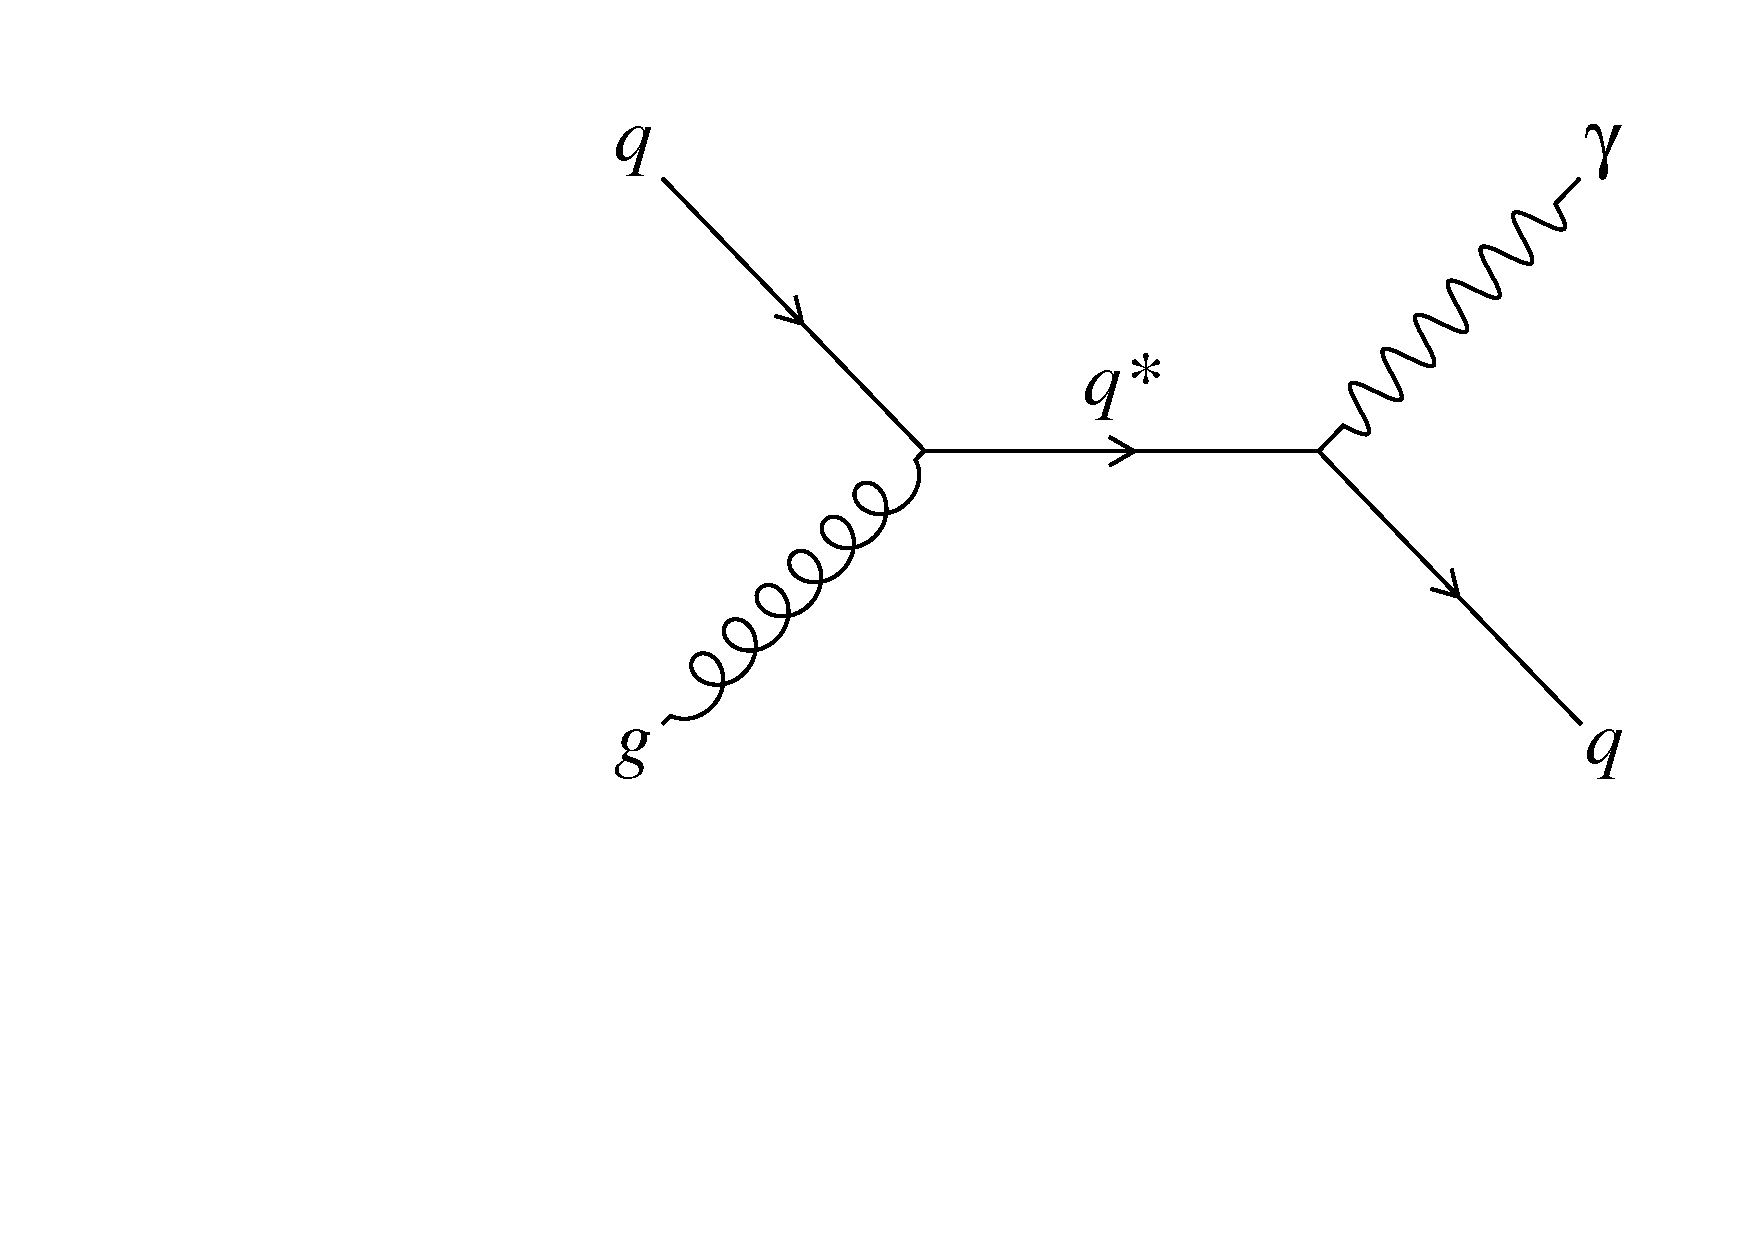
\includegraphics[width=5cm]{Chapter4/Feynman_diagrams/Signal_qgFusion.pdf}}
\hspace{0.1 in}
\subfloat[t-channel]{\label{fig:qqbarAnni}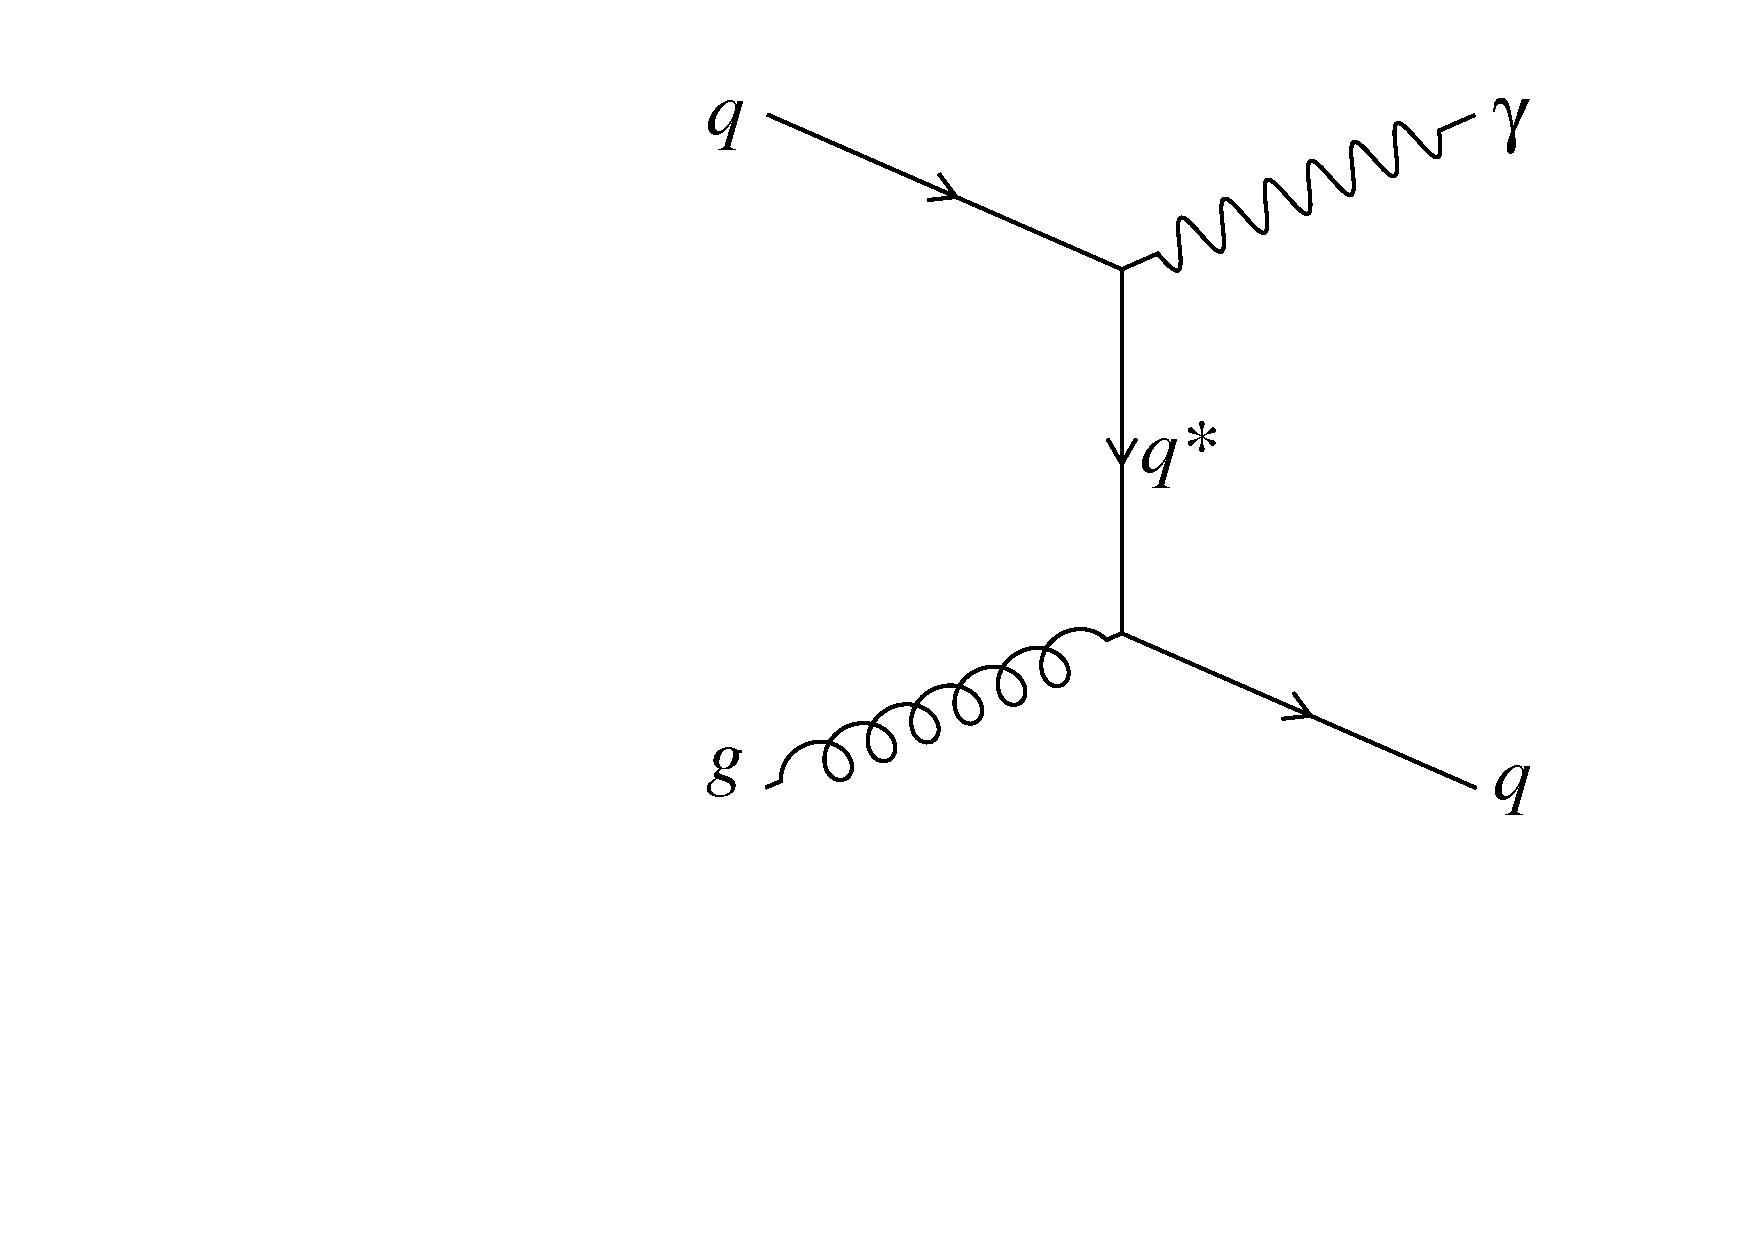
\includegraphics[width=5cm]{Chapter4/Feynman_diagrams/Signal_qgFusion_t.pdf}}
\hspace{0.1 in}
\caption{Feynman diagrams for quark-gluon fusion process in s and t channel.}
\label{fig:qgFusion_s_t}
\end{center}
\end{figure}
%\vspace{-0.2in}

The resonance will show its presence in the form of a bump in the s-channel and in the form of an excess of events in t-channel,
over the continuum invariant mass distribution of $\gamjet$.
\subsubsection{Backgrounds}
In pp collisions, the $\gamjet$ channel has a rather clean and simple signature within the detector. Still, many known SM processes can mimic this final state and
form the backgrounds of this study. These potential physics backgrounds are reported below as per their dominance:
\paragraph {\bf{SM $\gamjet$}}
\hspace{\parindent} The SM $\gamjet$ processes where a photon and a jet are produced in the hard collision, form the most dominant and irreducible
background for this study. A number of processes including quark-gluon compton scattering (qg $\rightarrow$ q$\gamma$), quark-antiquark annihilation (q$\bar{\textrm{q}}$
$\rightarrow$ g$\gamma$) and gluon-gluon fusion (gg $\rightarrow$ g$\gamma$) contribute to this background. The Feynman diagrams
representing these processes are shown in \fig{\ref{fig:GJ_Bkg}}. The qg scattering process dominates the total SM $\gamjet$ cross-section over the entire \pt range.
The contribution from the q$\bar{\textrm{q}}$ annihilation process is lesser, though it increases with increasing $\pt$. The gg fusion process, being a NLO process,
contributes negligibly. 

\vspace{-0.2in}
\begin{figure}[h!]
\centering
\subfloat[qg compton scattering]{\label{fig:qstarGJa}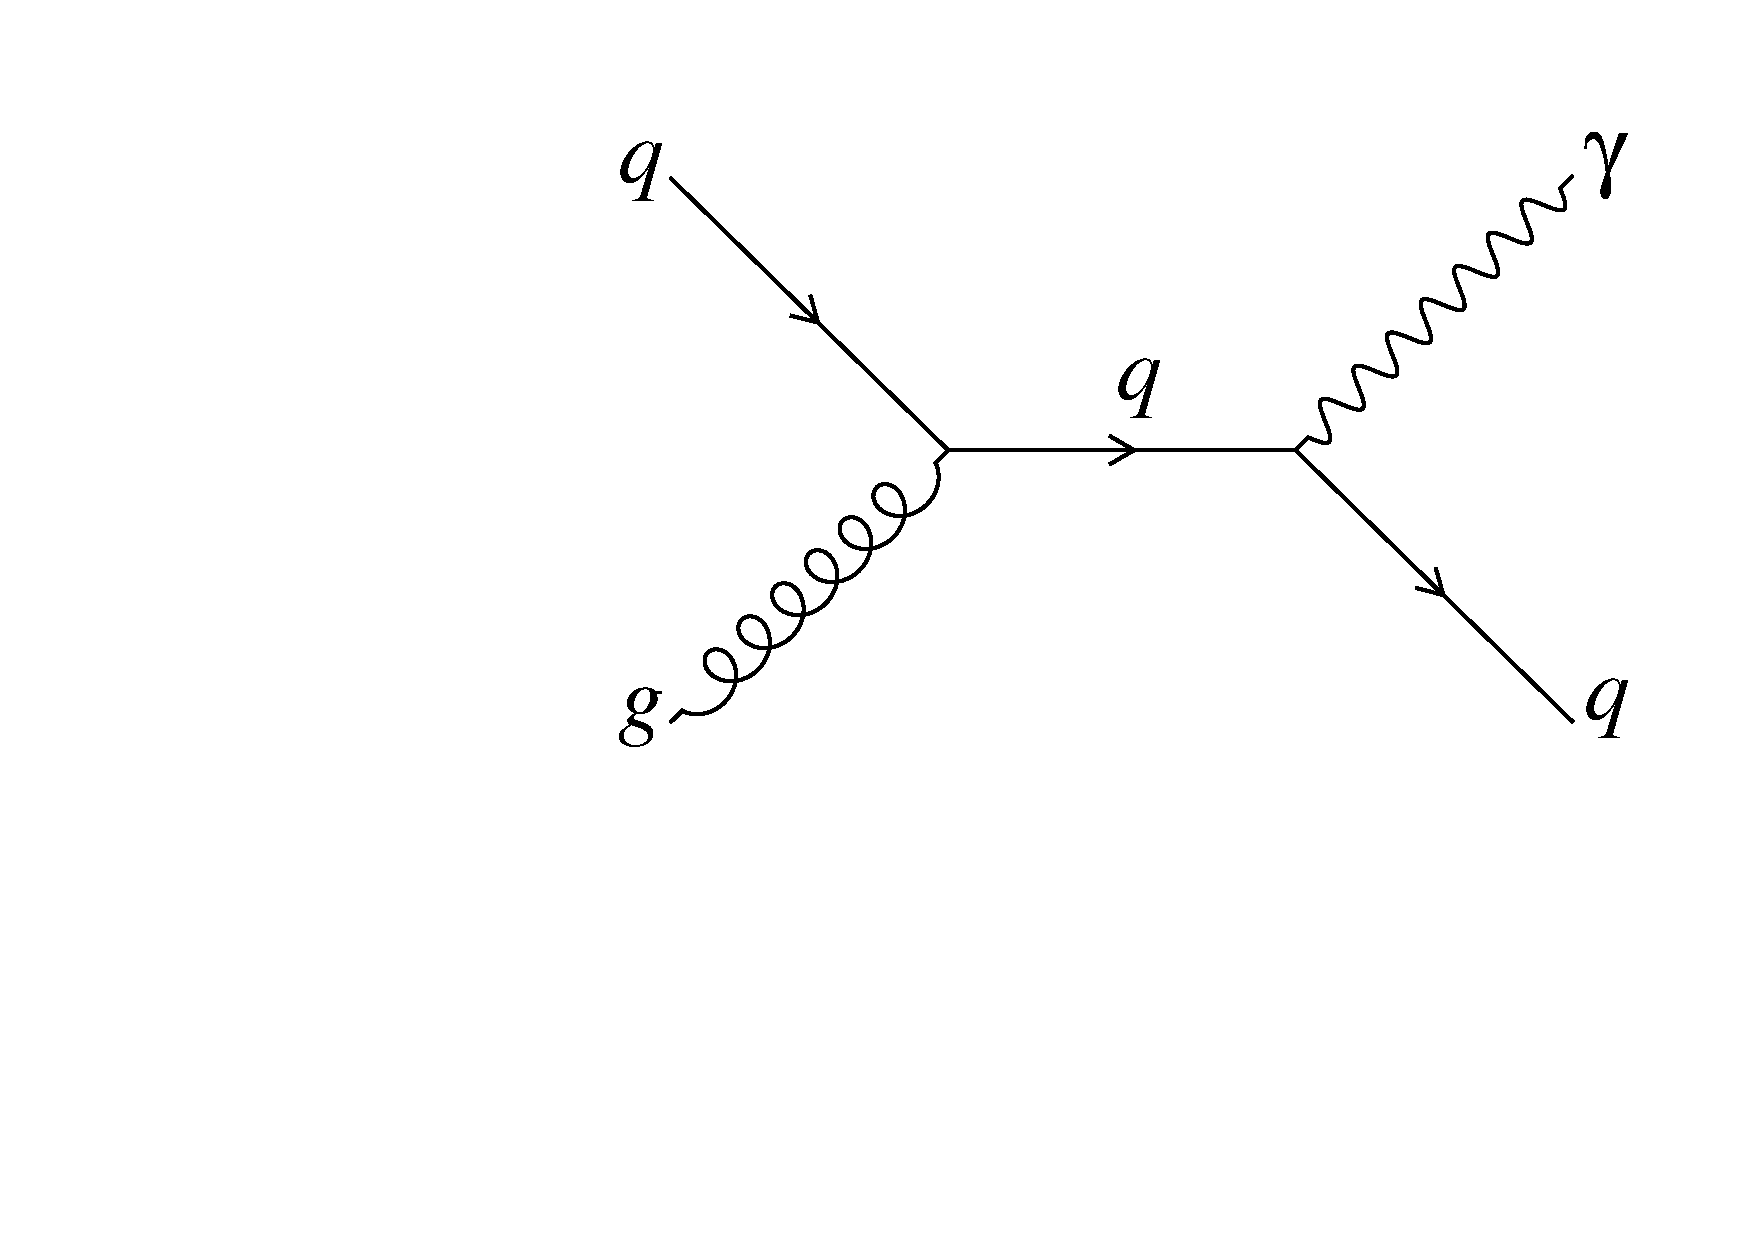
\includegraphics[width=4.4cm]{Chapter4/Feynman_diagrams/SMBkg_qgscattering.pdf}}
 \hspace{0.5cm}
 \subfloat[q$\bar{q}$ annihilation]{\label{fig:qstarGJb}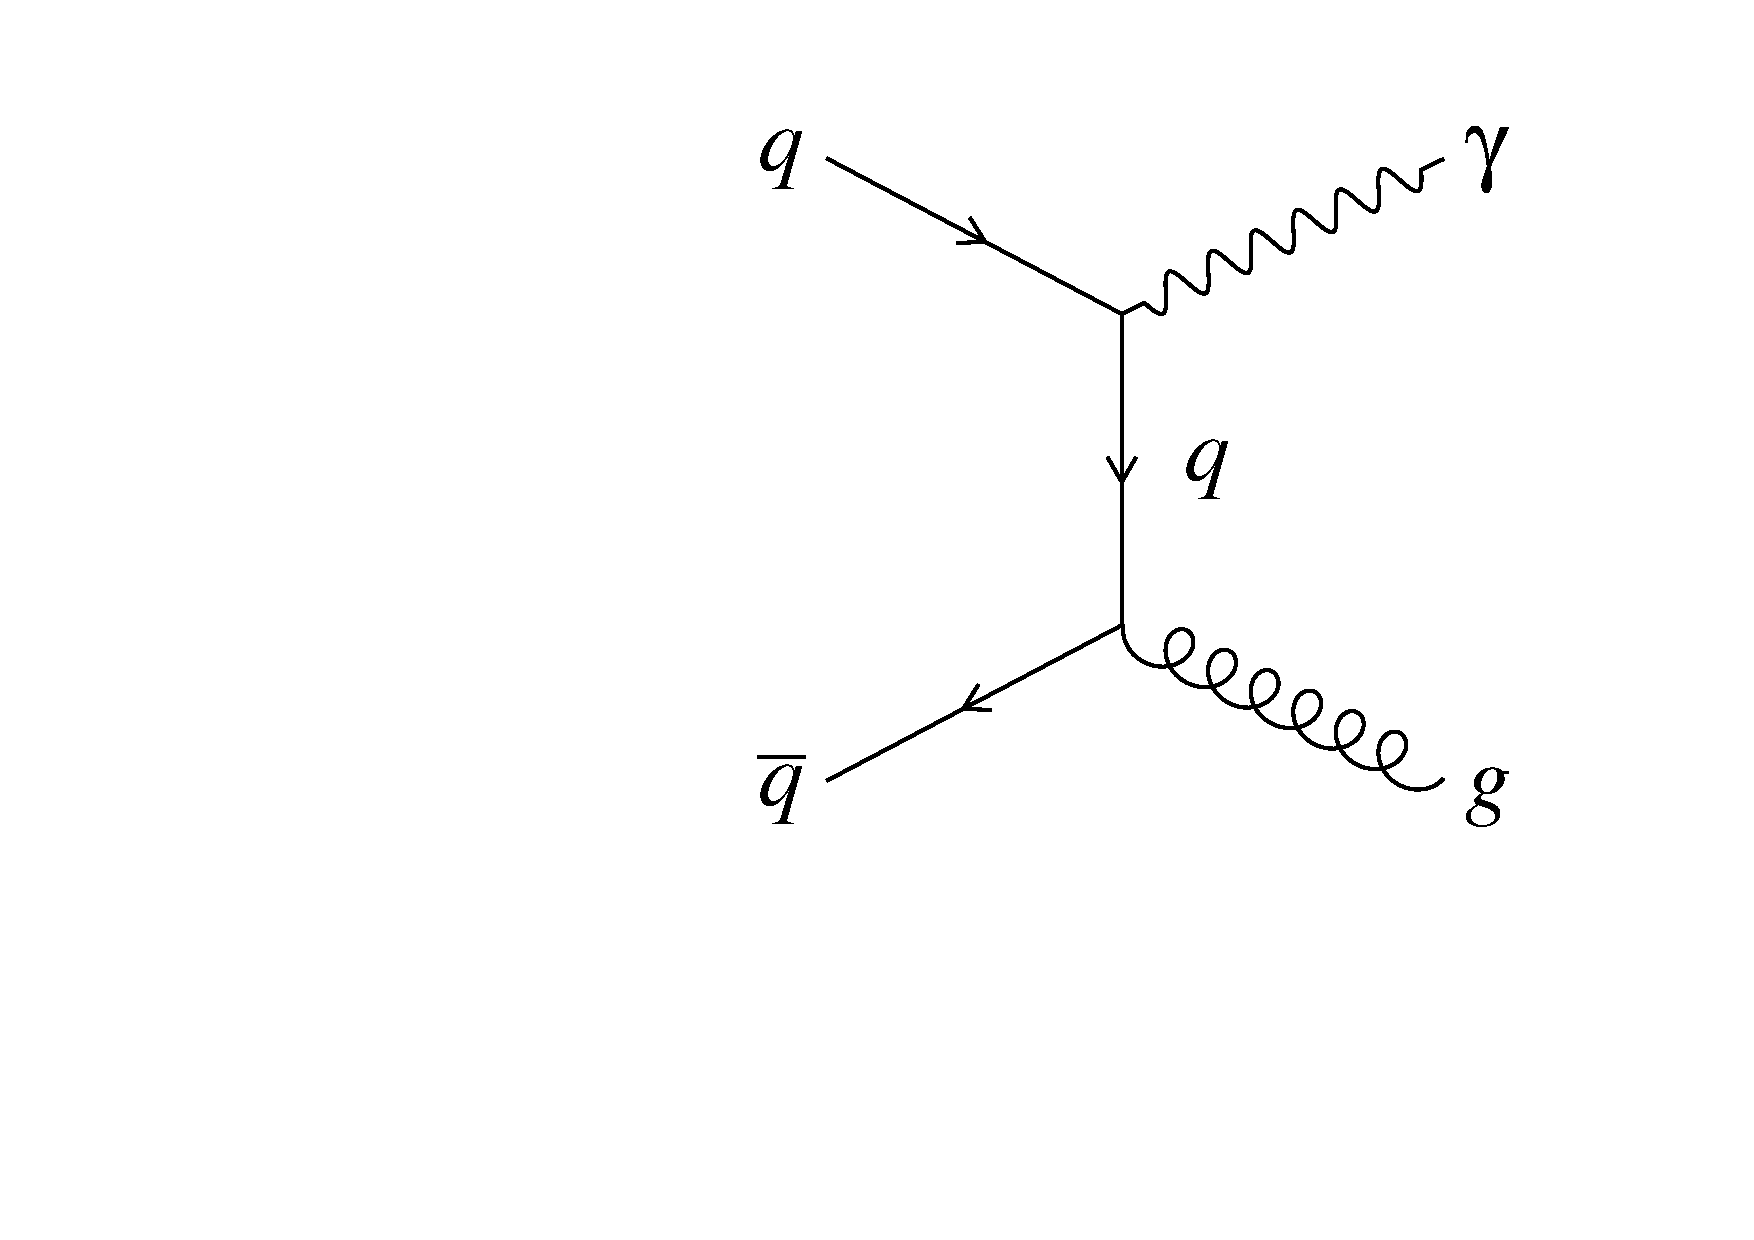
\includegraphics[width=4.4cm]{Chapter4/Feynman_diagrams/SMBkg_qqbarAnni.pdf}}
 \hspace{0.5cm}
 \subfloat[gg fusion]{\label{fig:qstarGJc}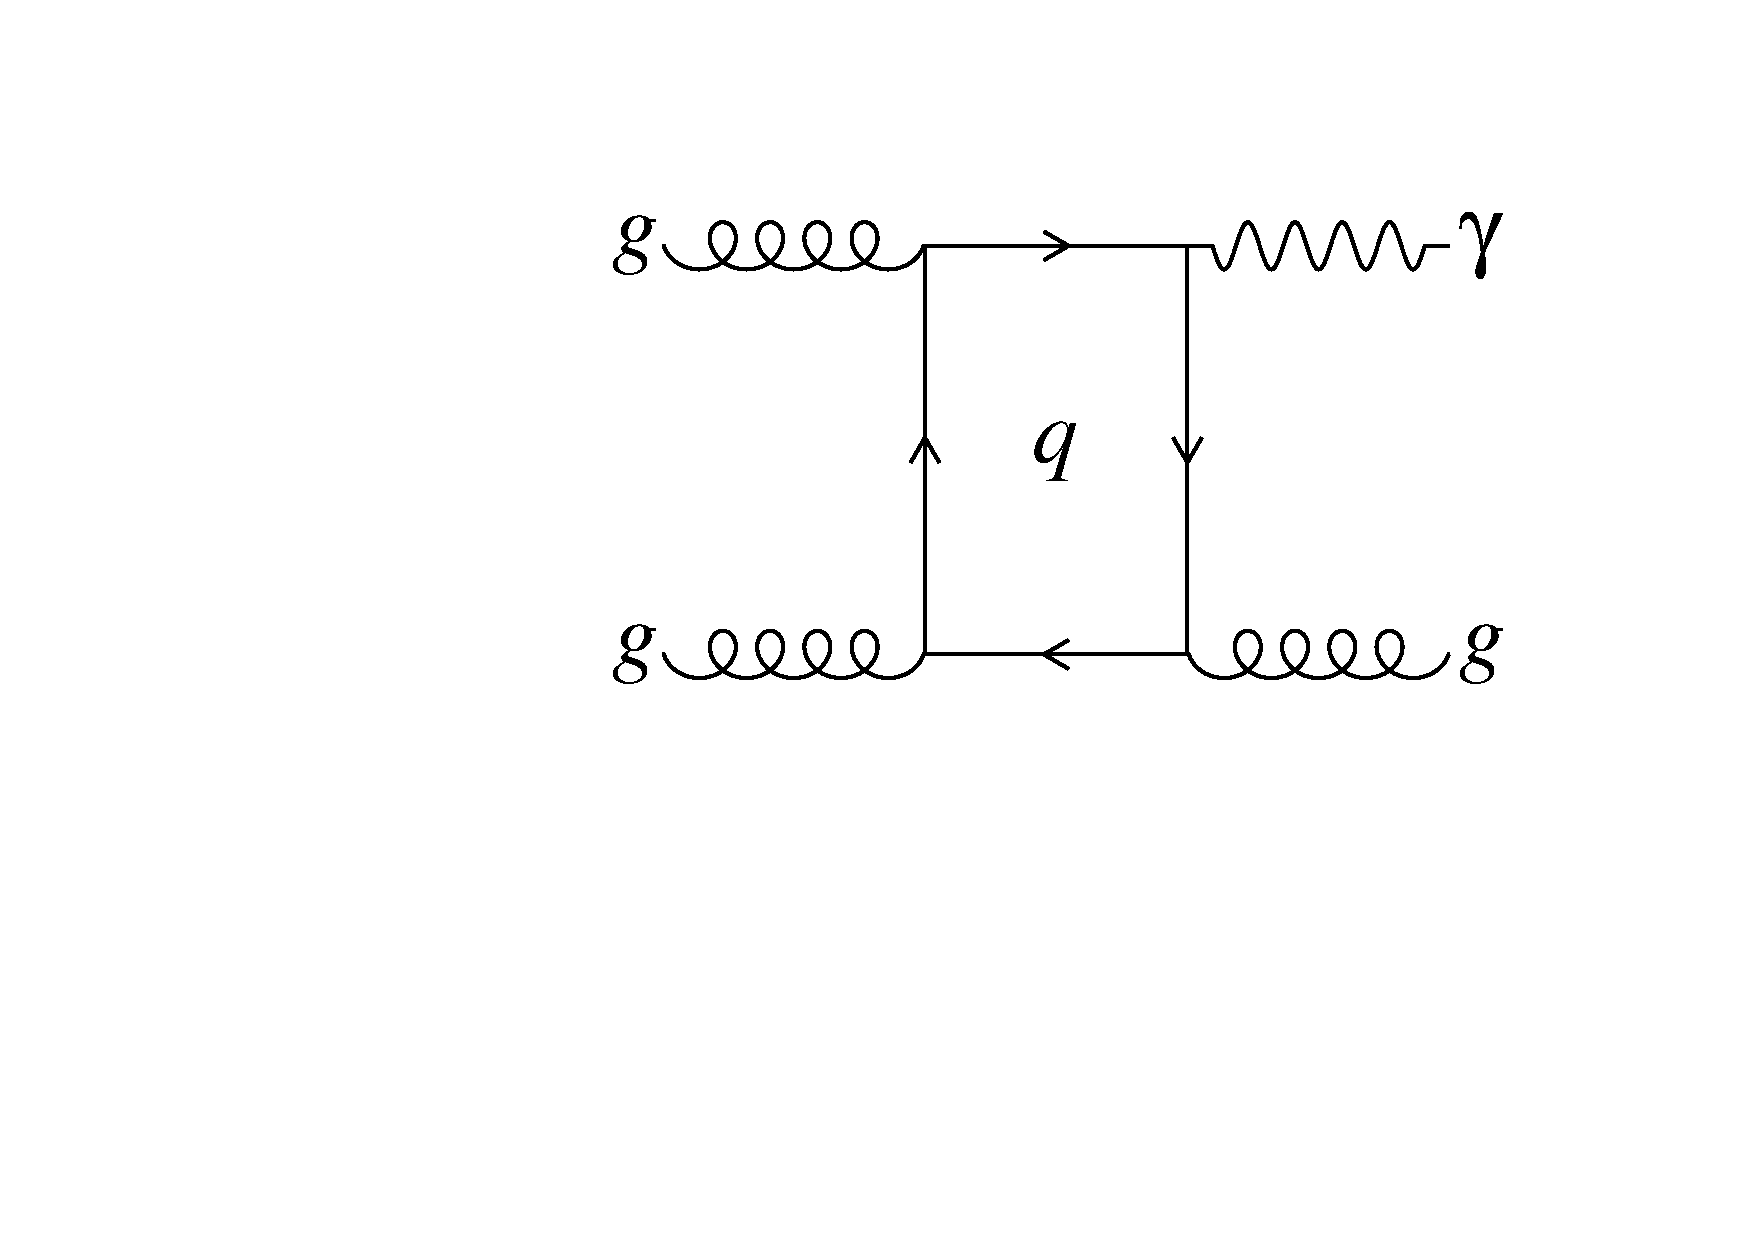
\includegraphics[width=4.4cm]{Chapter4/Feynman_diagrams/SMBkg_ggfusion.pdf}}
 \caption{Standard model background contribution from $\gamjet$ processes.}
\label{fig:GJ_Bkg}
\end{figure}
\paragraph {\bf{QCD dijet}}
\hspace{\parindent} The SM dijet processes where two jets are produced in the hard scattering, can form a background to a $\gamjet$ process if one of the jets fragments
into a highly energetic $\pi^{0}$ which then decays into a pair of overlapping photons and gets reconstructed as a single photon in the detector.
A number of processes like the ones shown in \fig{\ref{fig:QCDDijet_bkg}}, contribute to this background.
The production cross-section of these processes is around 10$^{4}$ times larger than the SM $\gamjet$ processes. But, since the probability of a jet faking a photon
is about $10^{-4} - 10^{-3}$, this background form the second largest background of this study. Also, the cross-section for these processes falls very swiftly
($\sim$ $\pt^{-4}$) with increasing $\pt$, so this background has significantly lower contribution at high $\pt$.

\begin{figure}[h!]
\centering
 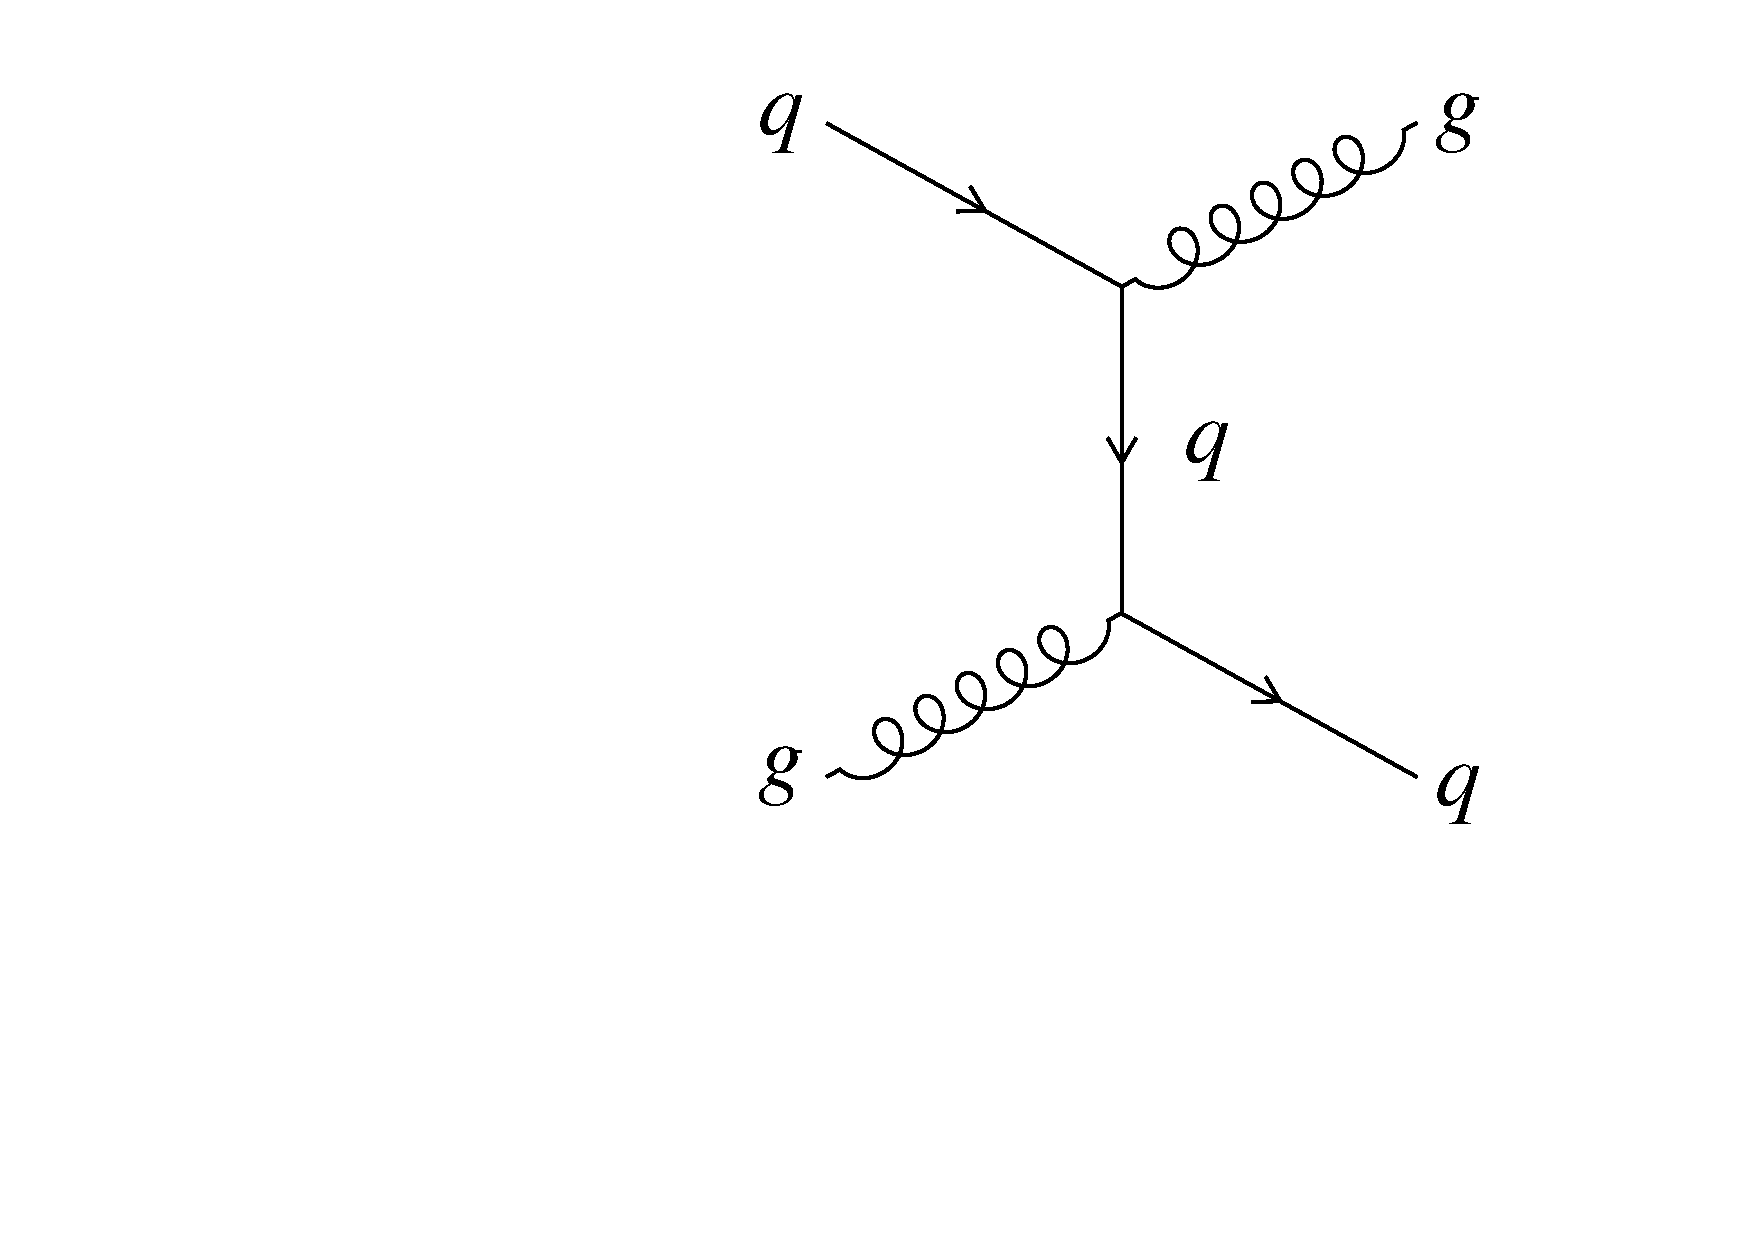
\includegraphics[width=4.4cm]{Chapter4/Feynman_diagrams/QCDBkg_gqTogq.pdf}
 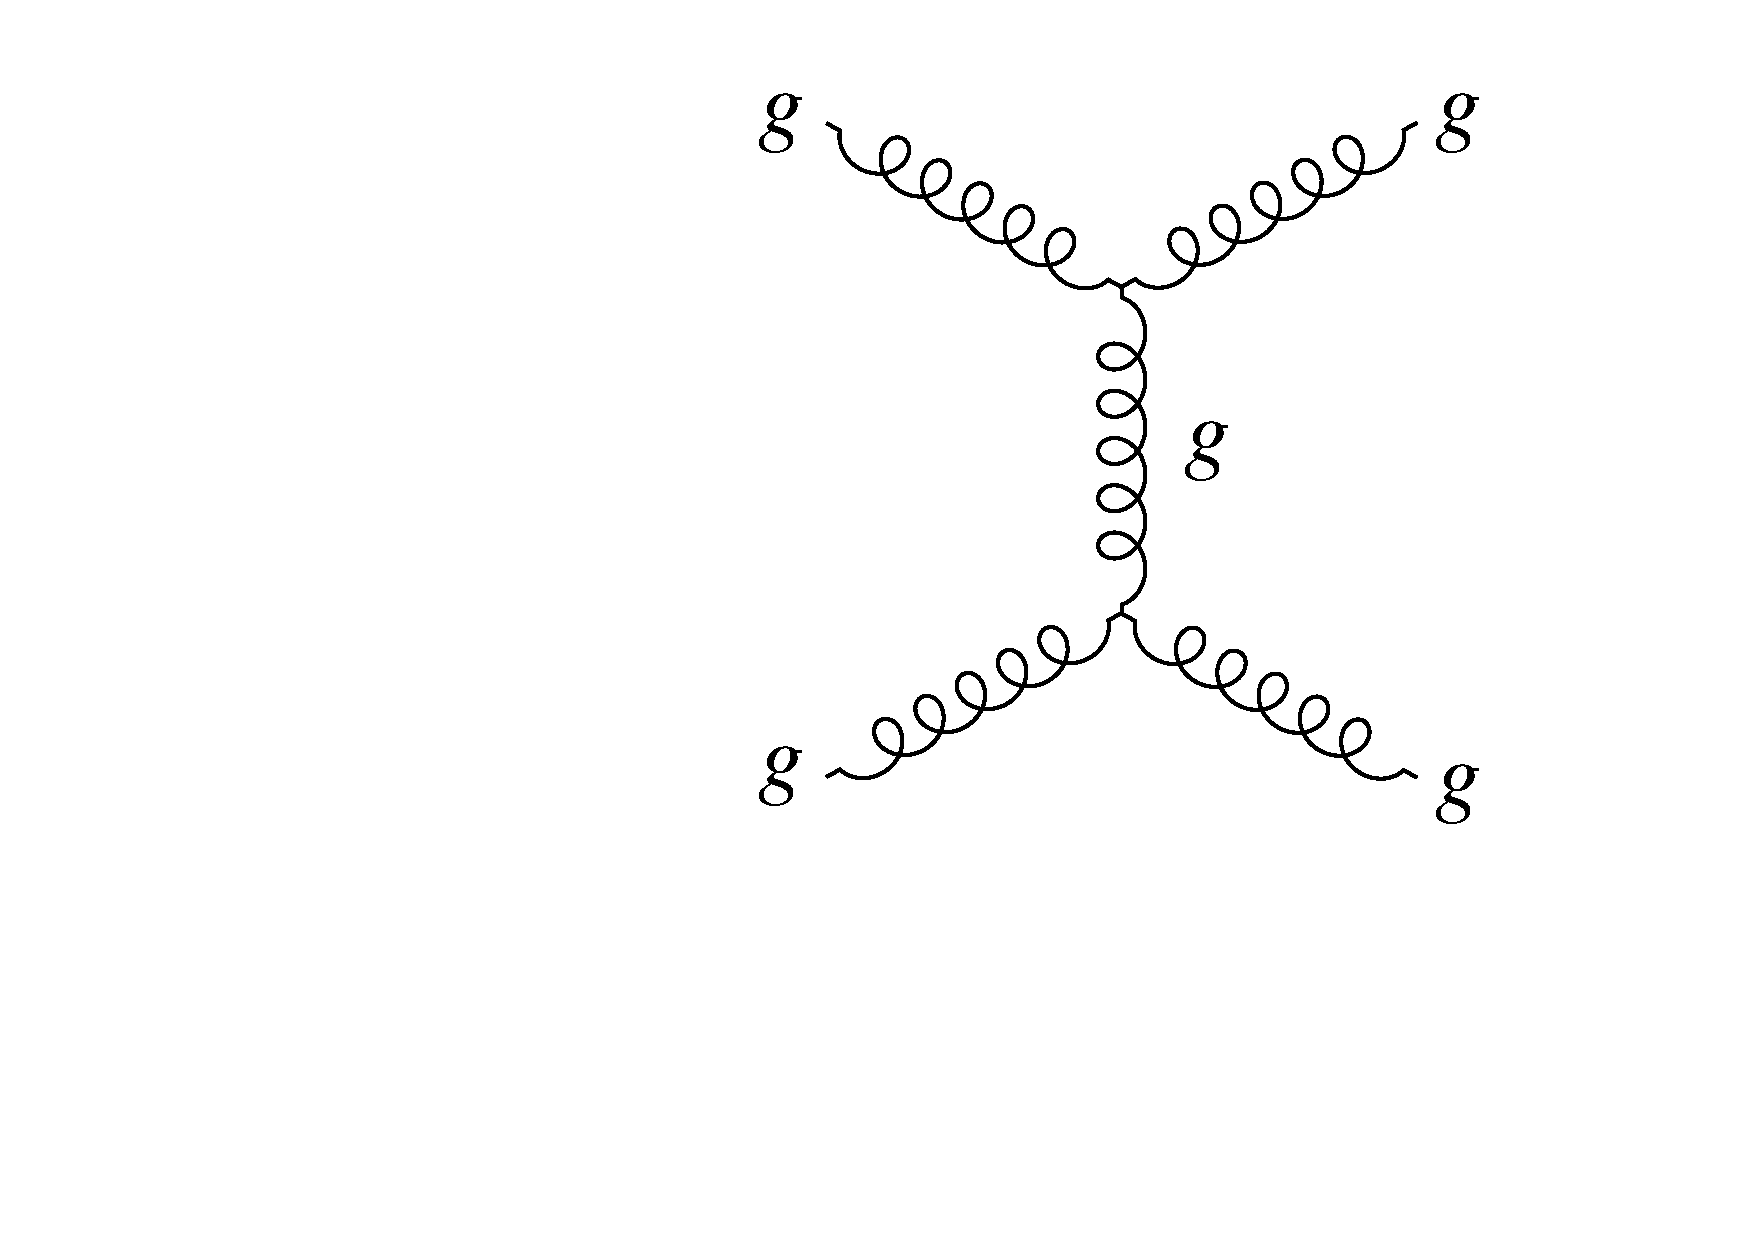
\includegraphics[width=4.4cm]{Chapter4/Feynman_diagrams/QCDBkg_ggTogg_T.pdf}\\
 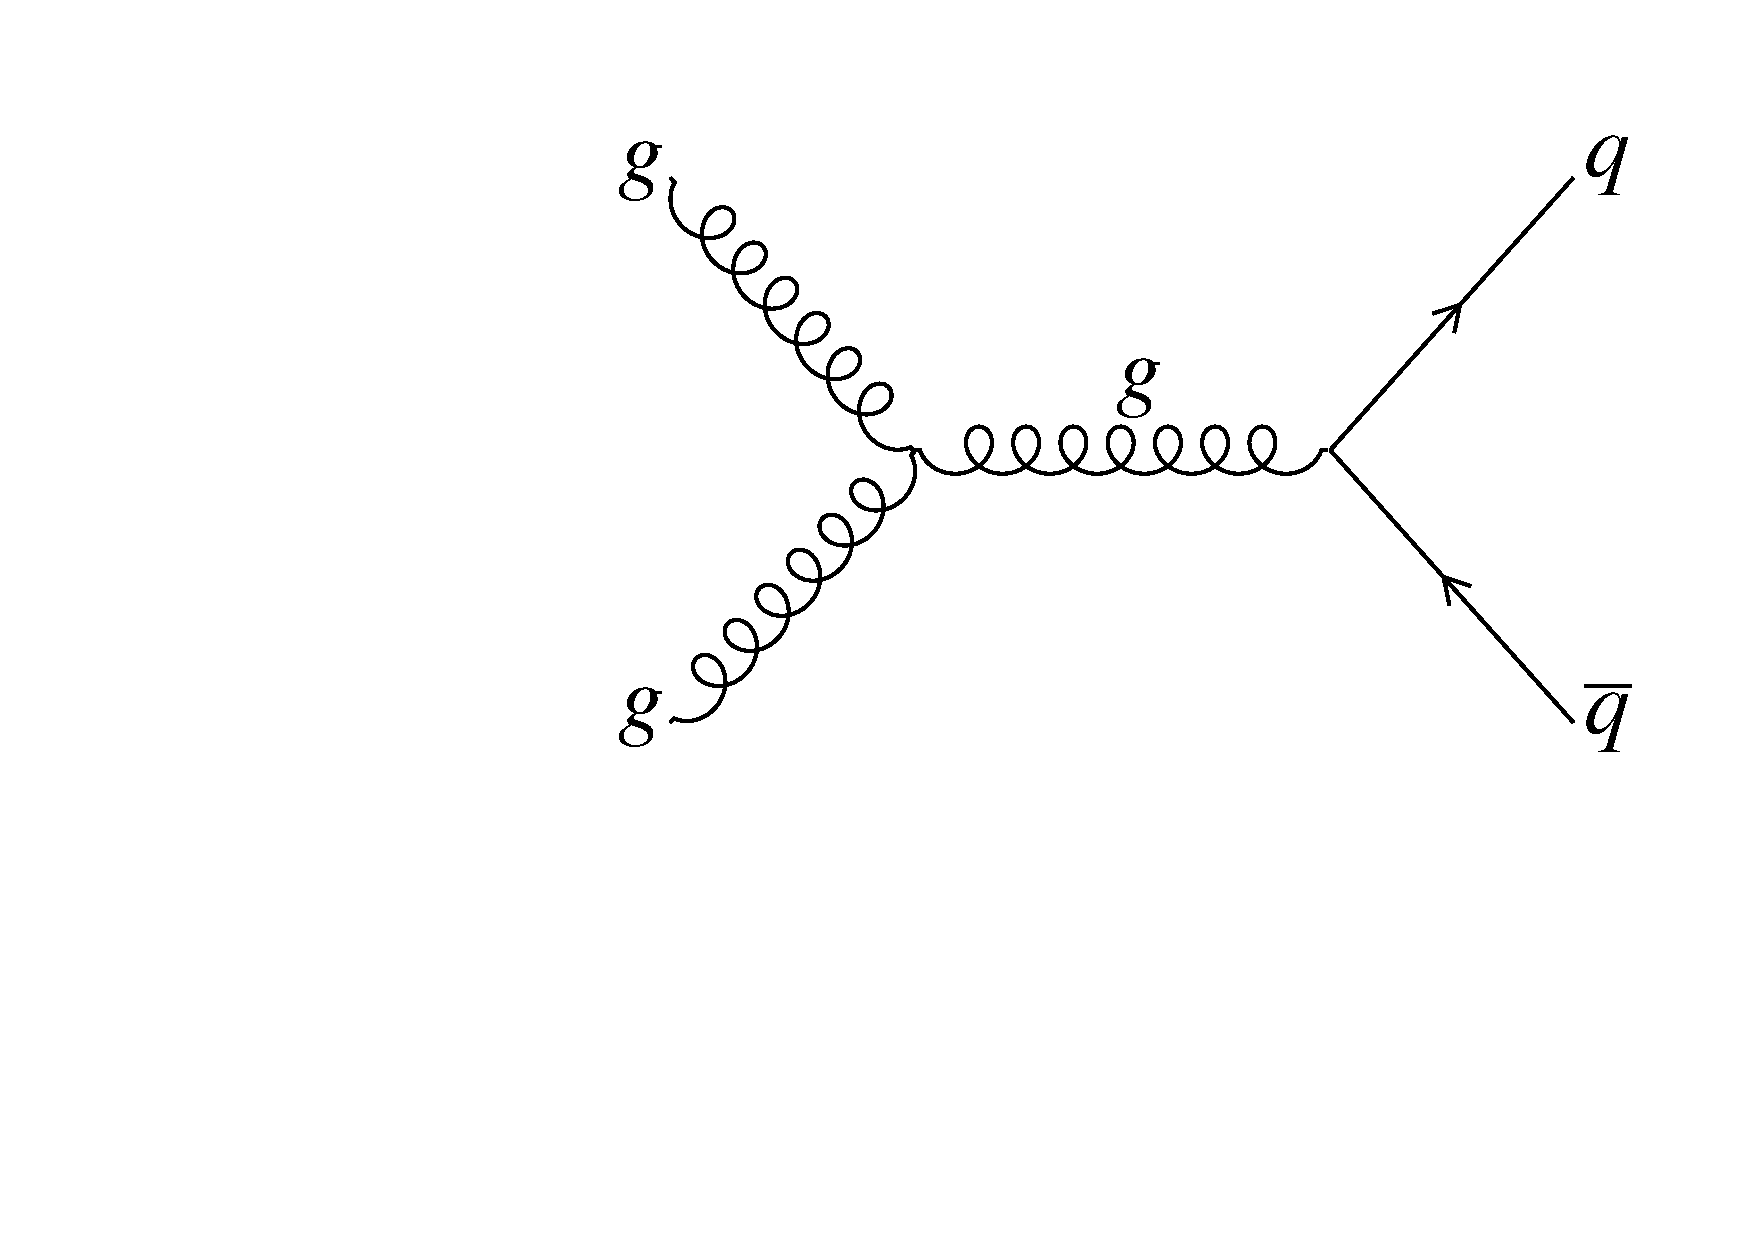
\includegraphics[width=4.4cm]{Chapter4/Feynman_diagrams/QCDBkg_ggToqqbar_S.pdf}
 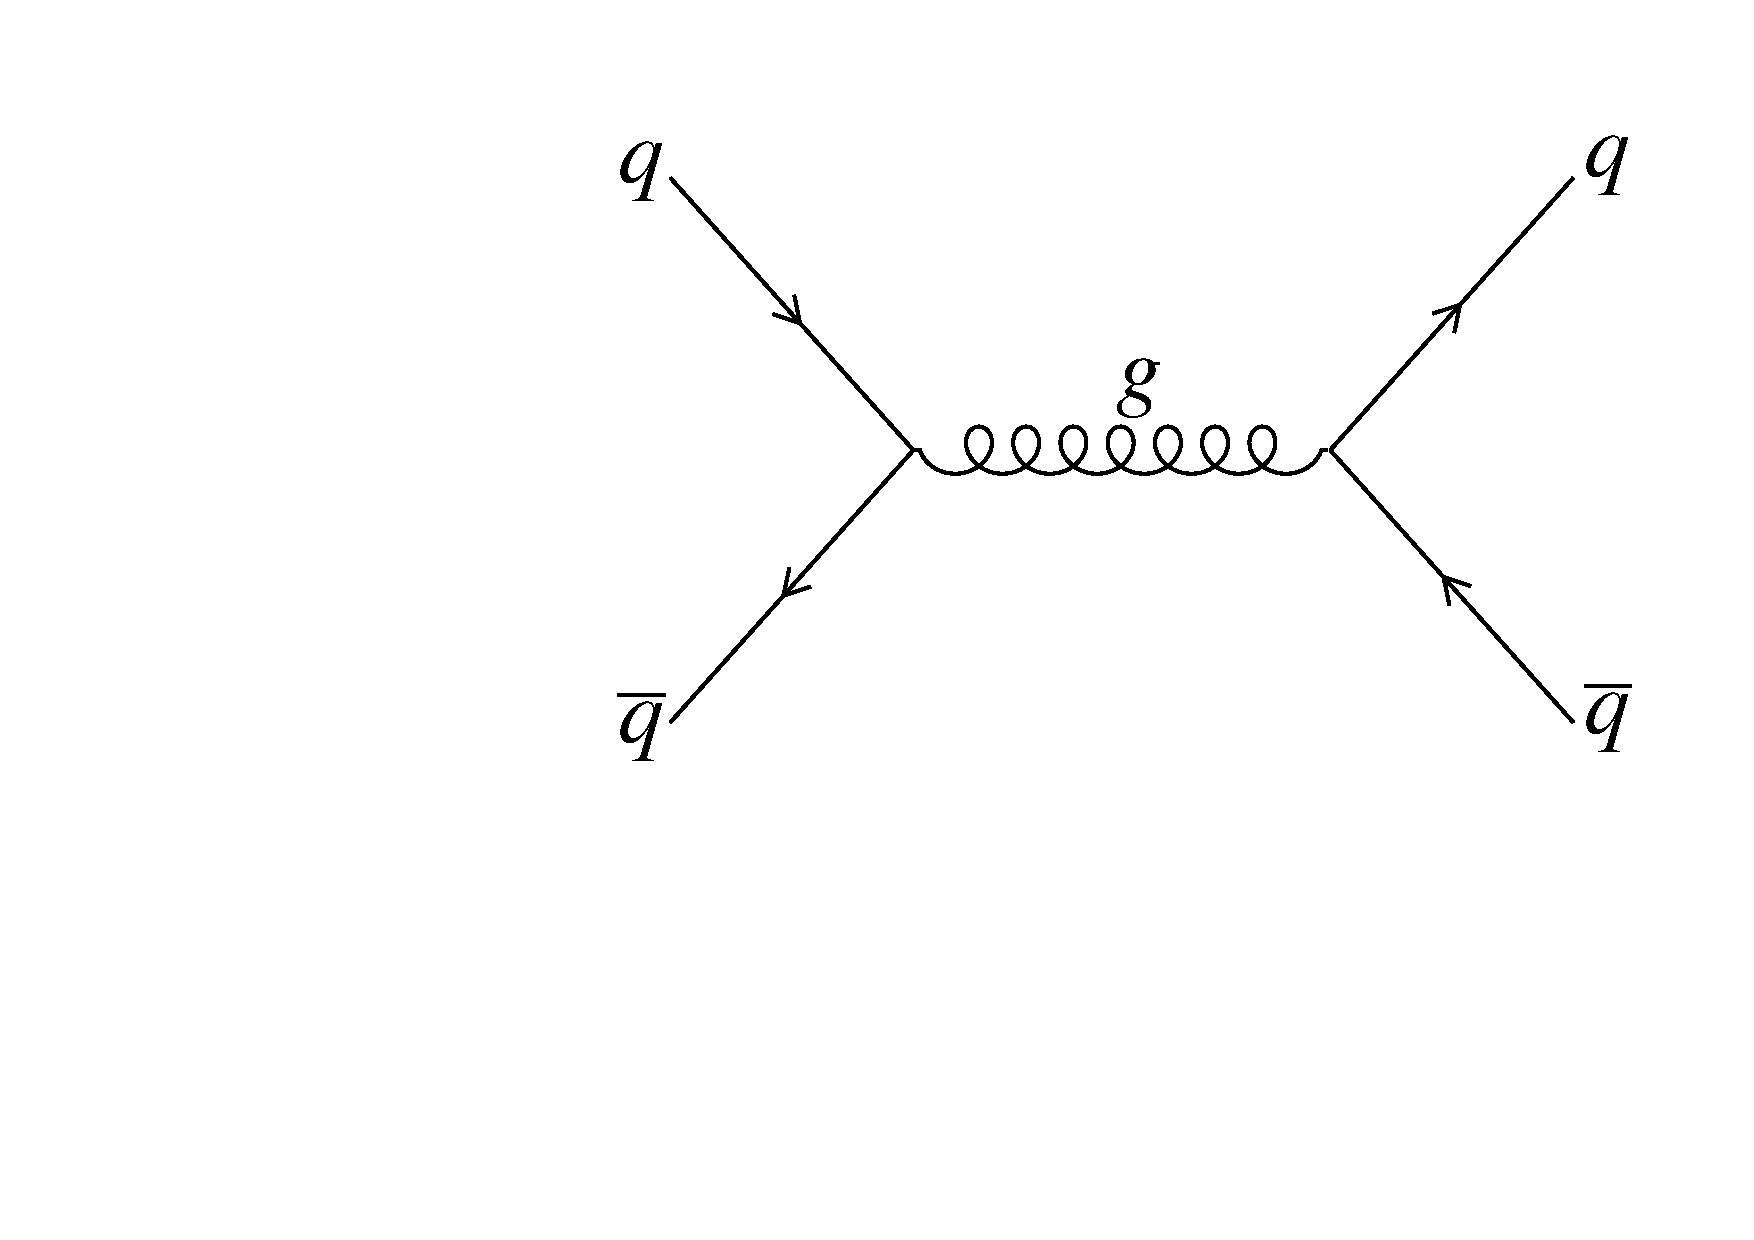
\includegraphics[width=4.4cm]{Chapter4/Feynman_diagrams/QCDBkg_qqbarToqqbar_S.pdf} 
 \caption{Standard model background contribution from  QCD dijet processes.}
\label{fig:QCDDijet_bkg}
\end{figure}
\vspace{-0.1in}

This background is also supplemented by the bremsstrahlung process where a photon is radiated by one of the initial or final state quarks
as shown in \fig{\ref{fig:QCDBreh_bkg}}. This results into one photon and two jets in the final state and can mimic a $\gamjet$ process if one of the jets is
lost or mismeasured. However, since these photons do not emerge from primary interaction vertex and have hadronic activity
in close vicinity, these can be easily removed by the photon isolation requirements.

\begin{figure}[h!]
\centering
  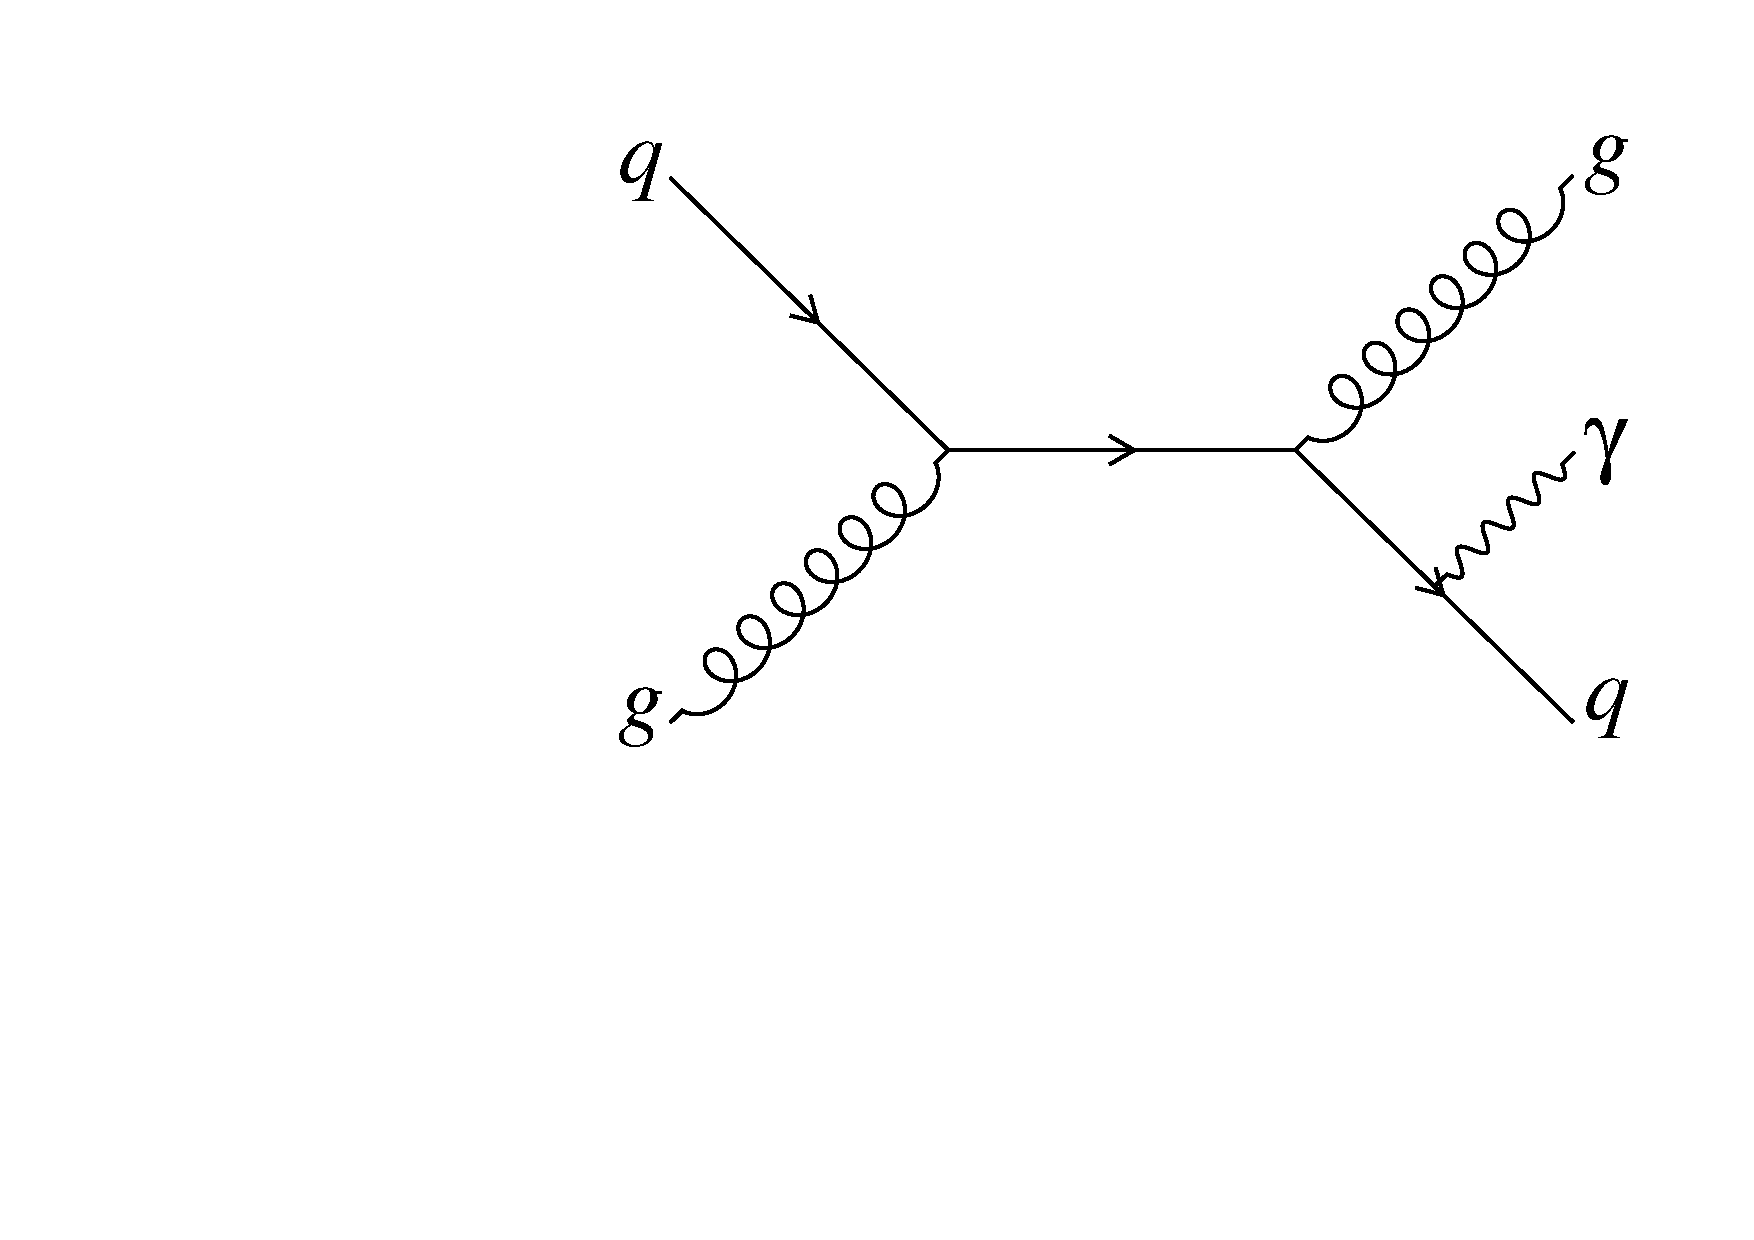
\includegraphics[width=4.4cm]{Chapter4/Feynman_diagrams/QCDBreh_qgToqgGamma_S.pdf}
  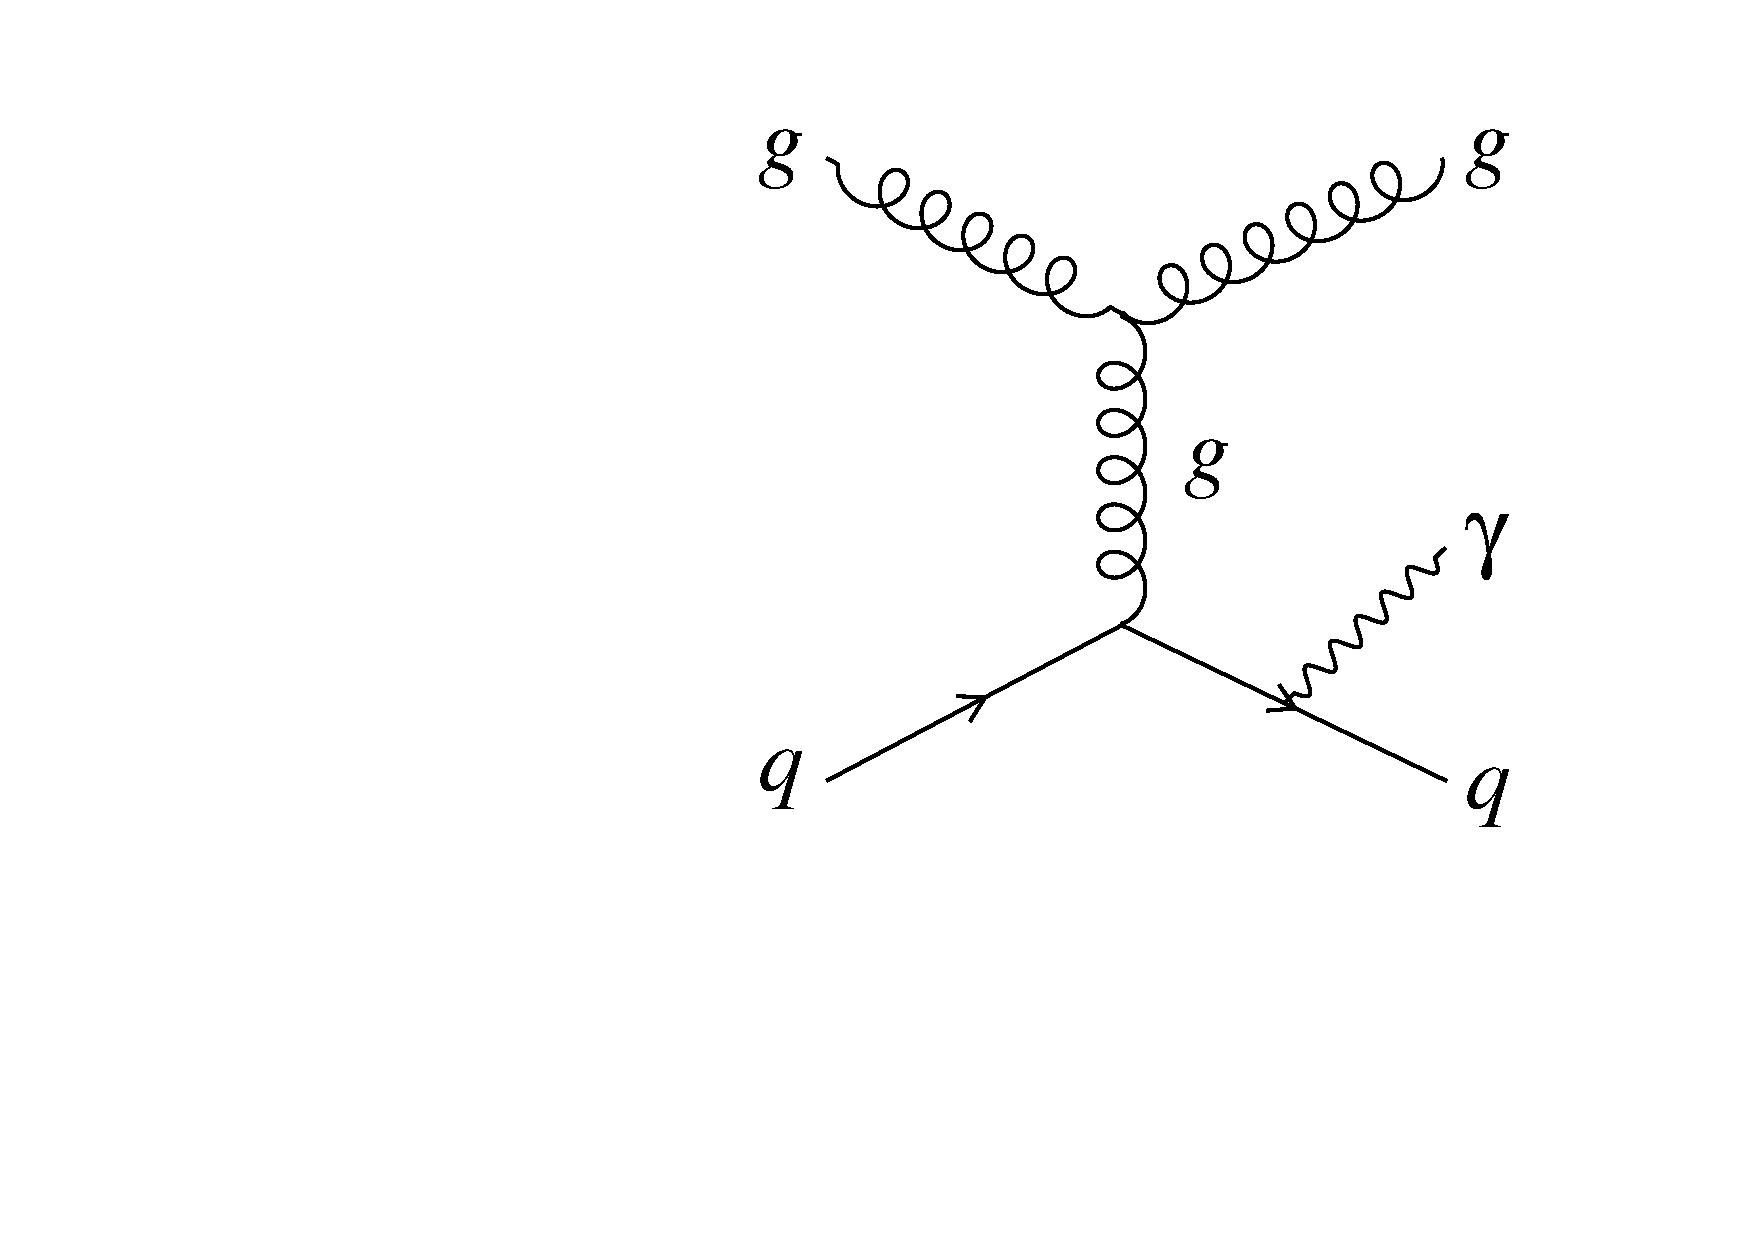
\includegraphics[width=4.4cm]{Chapter4/Feynman_diagrams/QCDBreh_qgToqgGamma_T.pdf}\\
  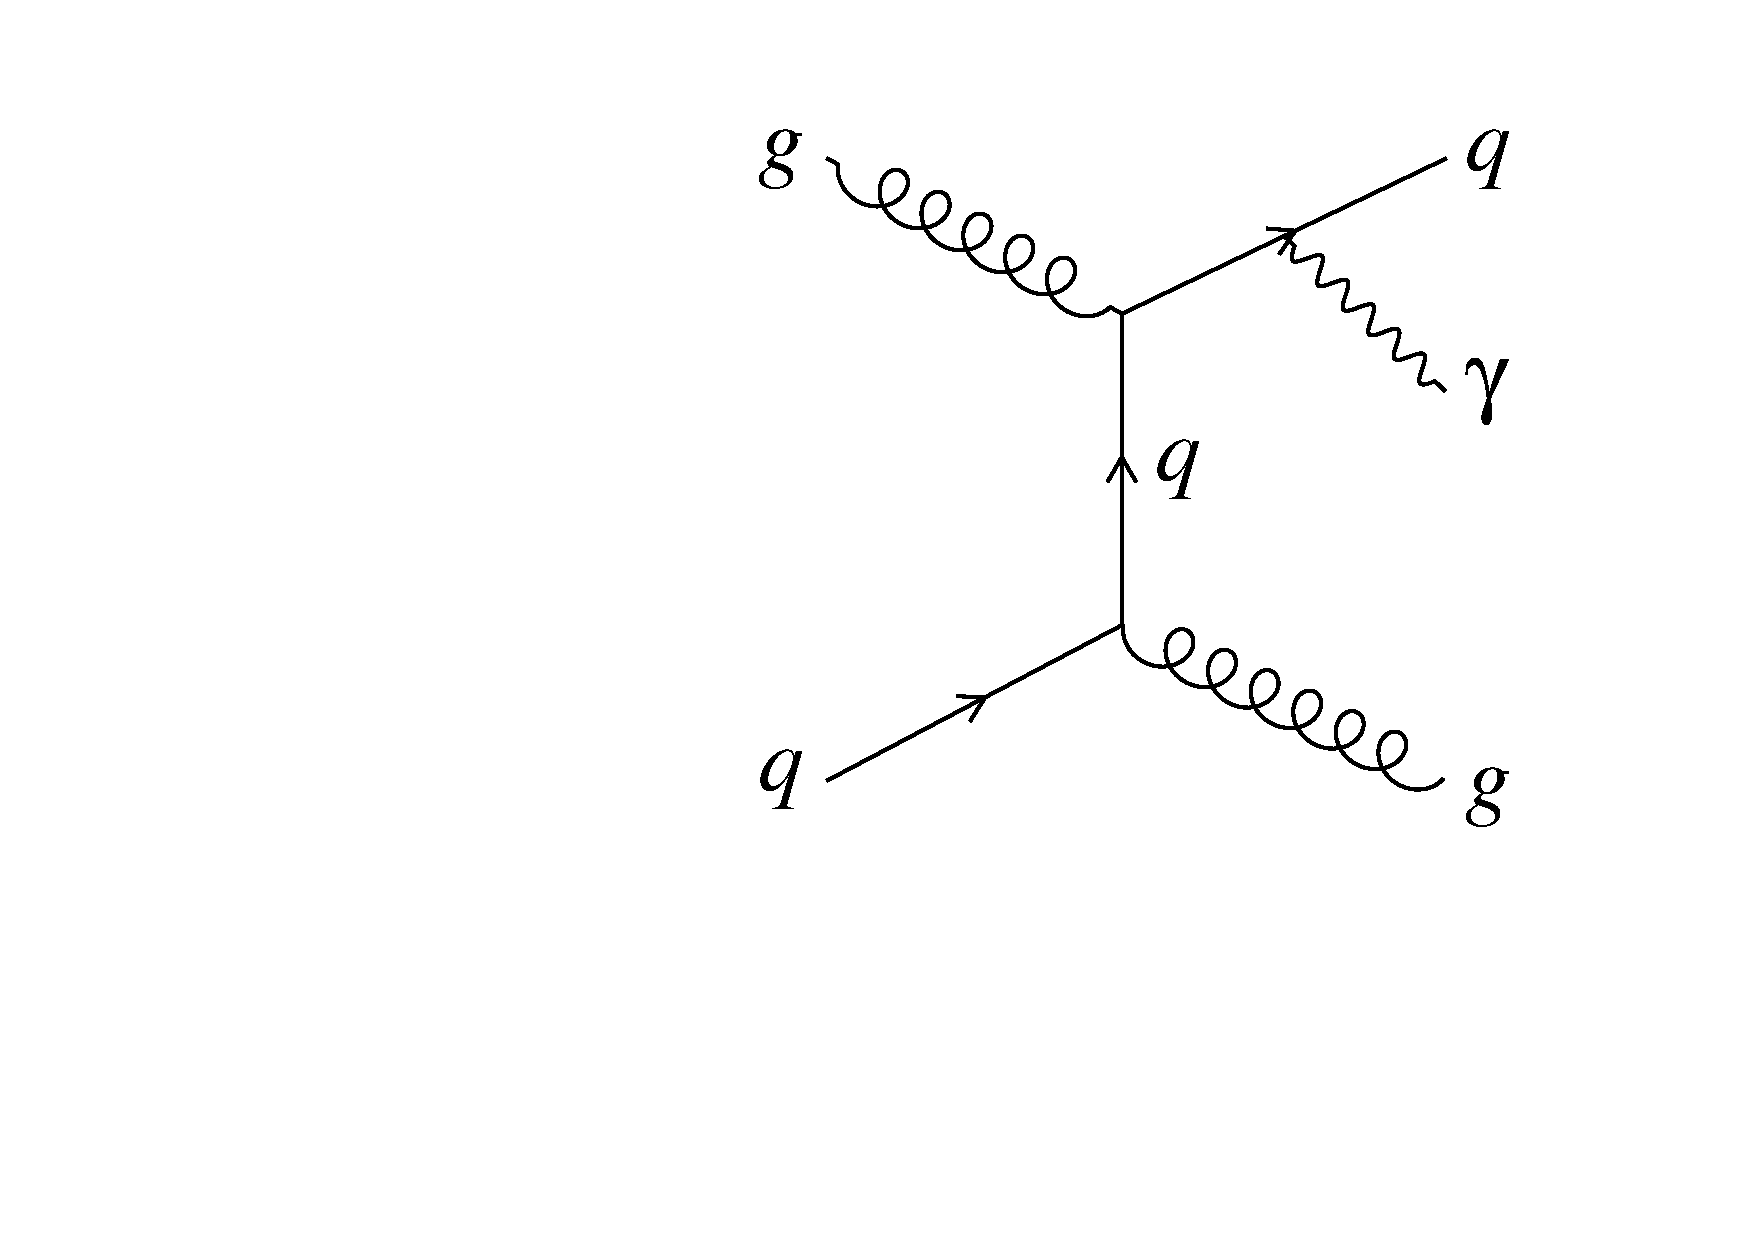
\includegraphics[width=4.4cm]{Chapter4/Feynman_diagrams/QCDBreh_qgToqgGamma2_T.pdf}
  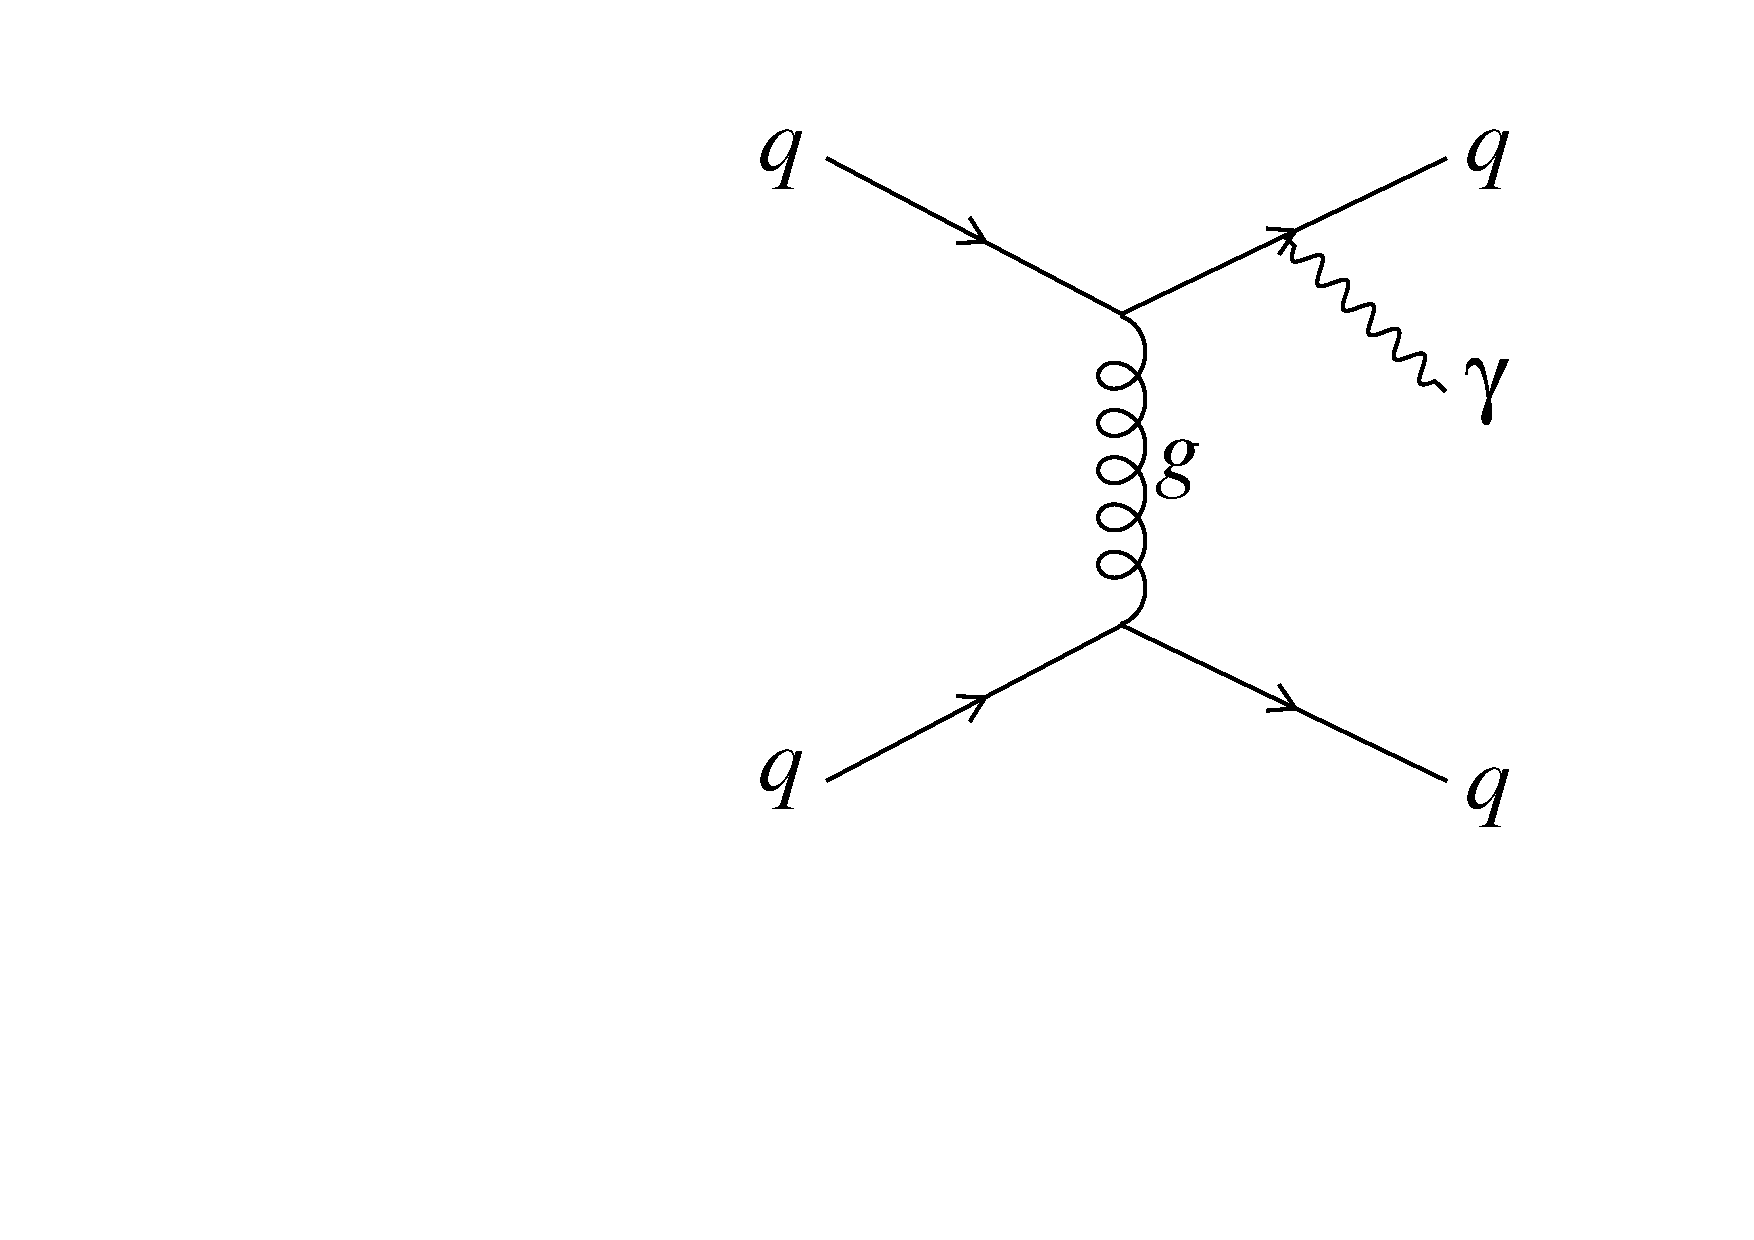
\includegraphics[width=4.4cm]{Chapter4/Feynman_diagrams/QCDBreh_qqToqqGamma_T.pdf}
 \caption{Bremsstrahlung contribution to SM QCD dijet production.}
\label{fig:QCDBreh_bkg}
\end{figure}
\paragraph {\bf{EWK}}
\hspace{\parindent} The SM electroweak processes, like W$/$Z $+$ jet production,
can contribute a small fraction to the total background when the heavy electroweak
boson decays leptonically and one of the leptons is either lost or go away in the form of missing transverse energy.
The Feynman diagrams corresponding to these processes are shown in
\fig{\ref{fig:EWK_bkg}}

\begin{figure}[h!]
\centering
 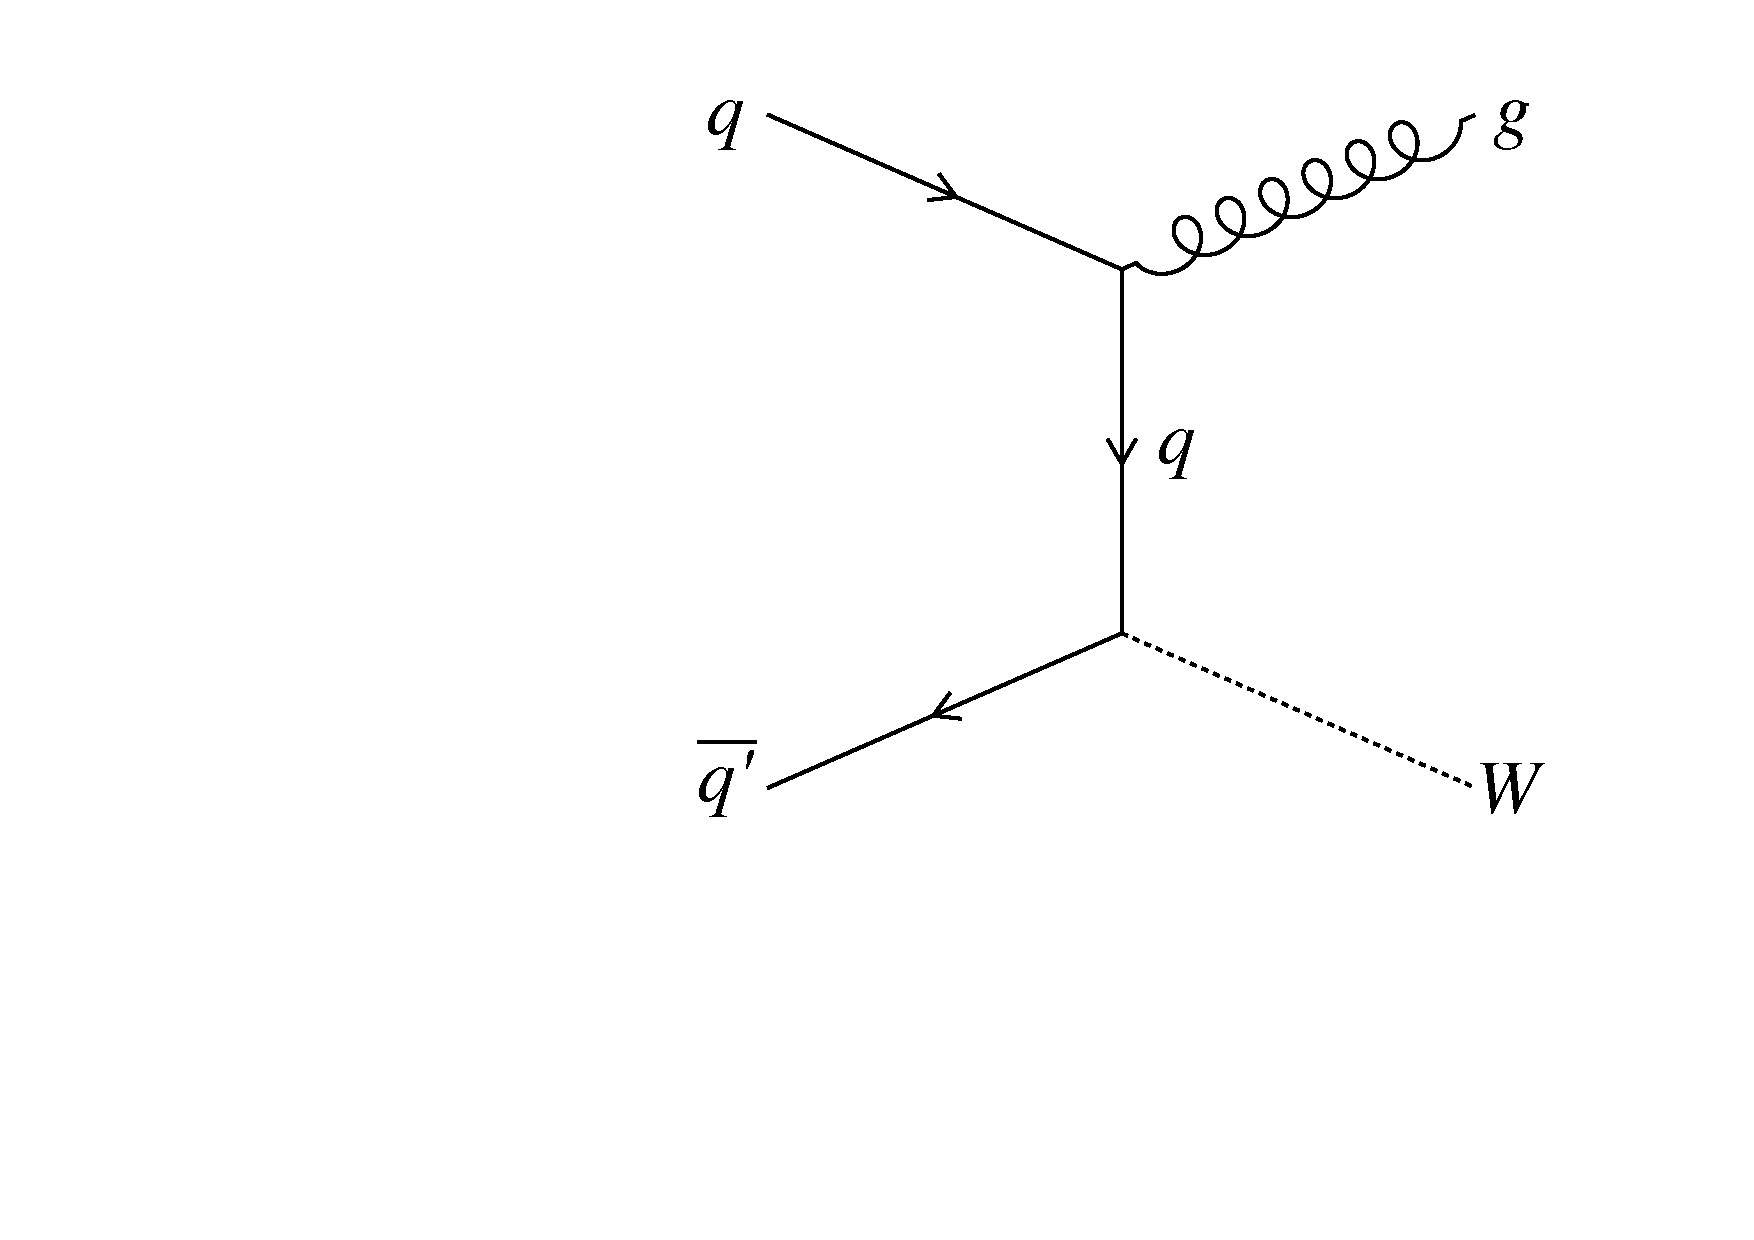
\includegraphics[width=4.4cm]{Chapter4/Feynman_diagrams/EWK_qqbarTogW.pdf}
 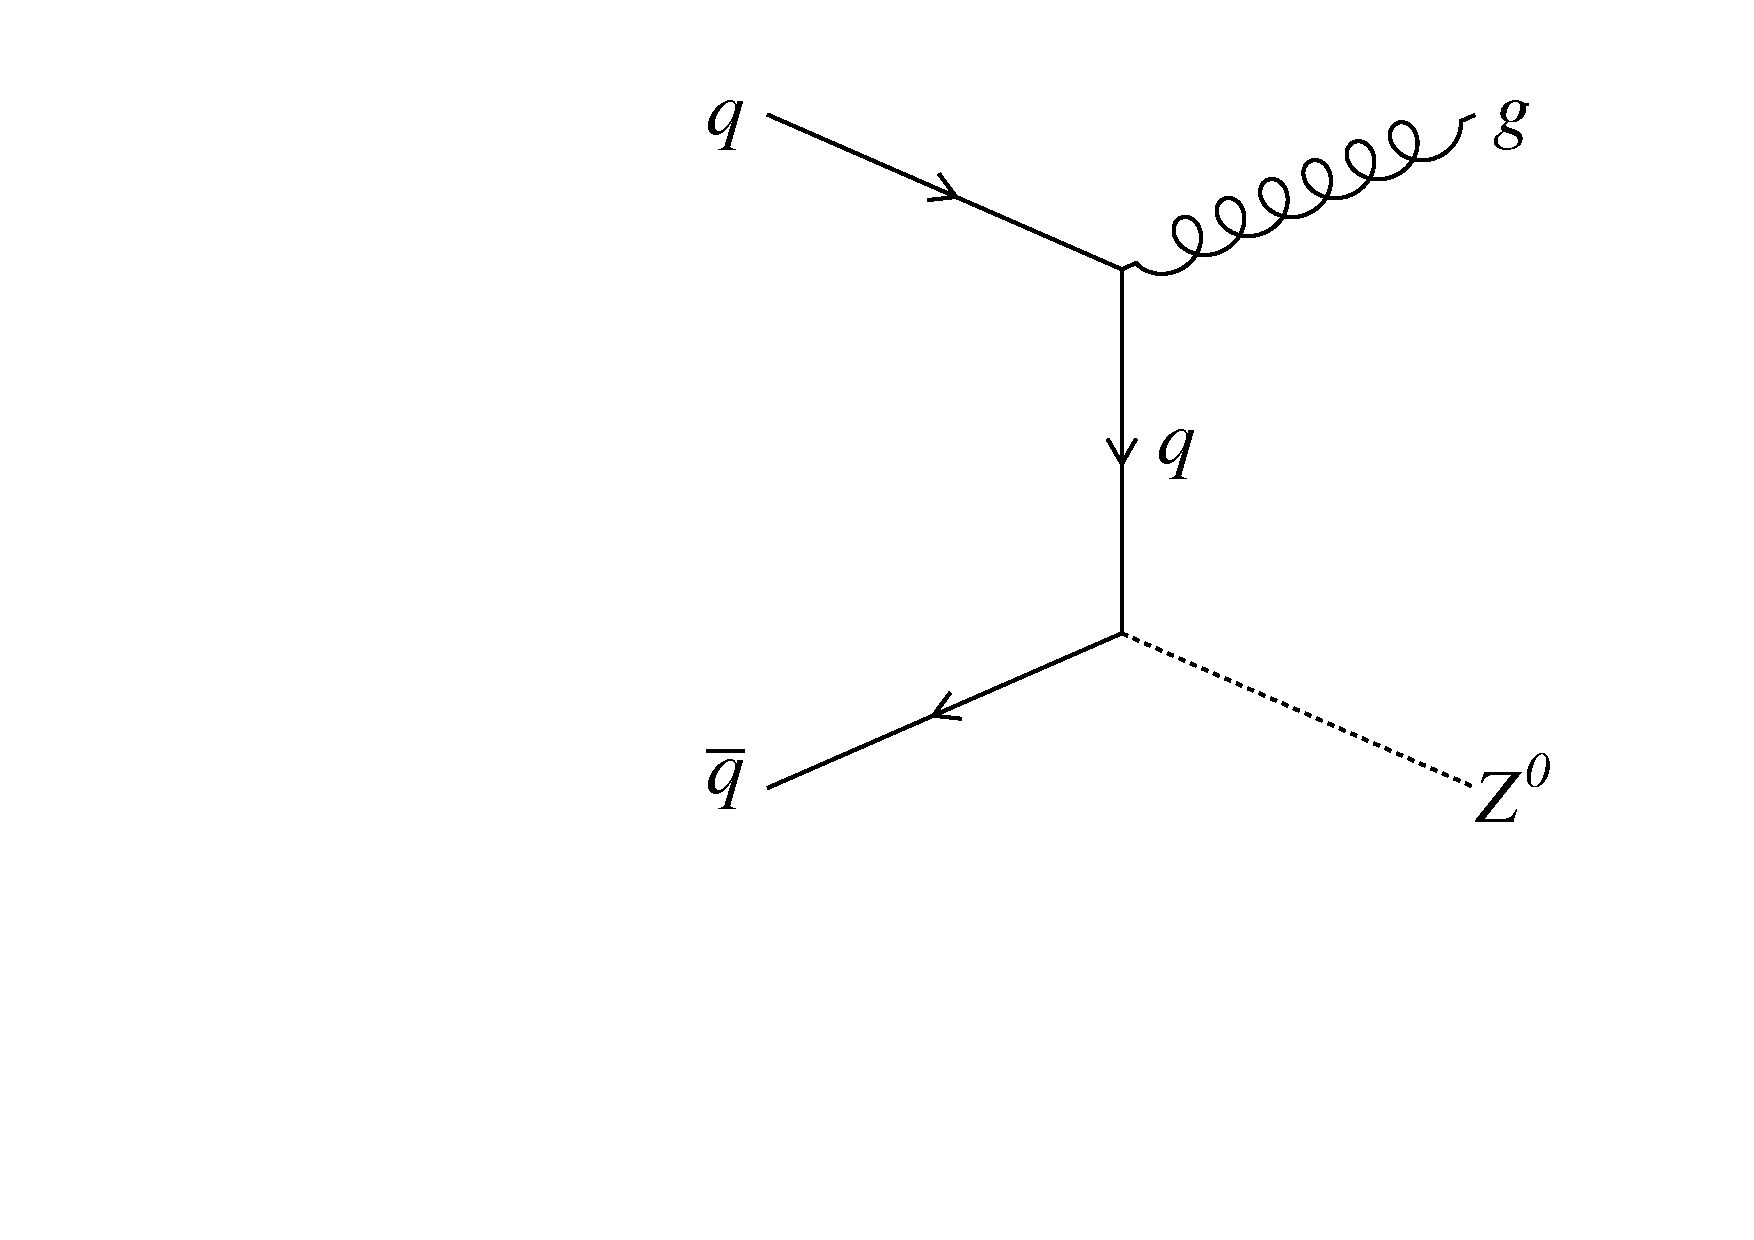
\includegraphics[width=4.4cm]{Chapter4/Feynman_diagrams/EWK_qqbarTogZ.pdf}
 \caption{Background contributions from electroweak processes.}
\label{fig:EWK_bkg}
\end{figure}
\vspace{-0.3in}
\section{Production of Ntuples}
The analysis chain starts with the production of Ntuples\footnote{Analysis specific event information extracted from the complete dataset and stored in
  ROOT files in the form of tree$/$branch structure.} of required data and MC samples. This step makes use of an analyzer, a code written mostly in C$++$ and python
within the CMSSW environment, that extracts the information, related to different physics objects, triggers, vertices, pile-up \etc, from the reconstructed or
simulated datasets and store them in ROOT files in
the form of Ntuples. Since the analyzer has to run over billions of events contained within a dataset,
this step is almost impossible to perform using interactive computing.
A technique known as grid computing~\cite{Eck:840543}, that considers a number of computer resources located at multiple places all over the world, is used along with
CMS Remote Analysis Builder (CRAB)\footnote{An official CMS tool that allows an end user to access the data distributed at various sites as well as automates the
  task of job submission.}~\cite{Sala:1358821} to achieve this task. The Ntuples consist of organized information of all the quantities required for further
analysis. This study has used the Tier-3 center present at Fermilab, USA, referred to as T3$\_$US$\_$FNALLPC, for the production, storage, and
analysis of data and MC Ntuples. 
\subsection{Samples processed}
The recorded detector data and simulated MC samples used in this analysis are detailed below. The MC samples include the signal as well as the background samples.
All the samples are used in mini-AOD format and have been processed using a CMSSW version $8\_0\_26\_\mathrm{patch}1$.
\subsubsection{Data}
This analysis used the pp collision data collected by the CMS detector at $\sqrtthirteentev$ in 2016, with a bunch crossing frequency of 25\unit{ns}.
This data corresponds to a total integrated luminosity of 35.9 \fbinv.
The reconstructed data in mini-AOD format, with only certified runs and luminosity sections selected using an official JSON\footnote{A JSON
  file is a special java format file that lists the good runs and luminosity sections collected with optimum detector
  conditions. The JSON files are located at the link:\\
  \scriptsize\url{https://cms-service-dqm.web.cern.ch/cms-service-dqm/CAF/certification/Collisions16/13TeV/ReReco/}} file, have been used.
The list of data samples split in different run era ranging from B to H and the name of JSON file are presented in \tab{\ref{Table:datasample}}.
%---------------TABLE FOR Data sample and  JSON-------------------
\begin{table}[h!]
  \begin{center}
    \resizebox{15cm}{!}{
      \begin{tabular}{lcc}
        \toprule
        \belowrulesepcolor{Mygray}
        \belowrulesepcolor{Mygray}
        \belowrulesepcolor{Mygray}
        \rowcolor{Mygray}[\dimexpr\tabcolsep+0.09pt\relax]
        \bf{Data Samples} & \bf{Run Range} & \bf{Luminosity (\fbinv)}\\
        \aboverulesepcolor{Mygray}
        \aboverulesepcolor{Mygray}
        \aboverulesepcolor{Mygray}
        \midrule
        /SinglePhoton/Run2016B-03Feb2017\_ver2-v2/MINIAOD & $273150 - 275376$ & 5.788 \\
        /SinglePhoton/Run2016C-03Feb2017-v1/MINIAOD       &  $275656 - 276283$ & 2.573 \\
        /SinglePhoton/Run2016D-03Feb2017-v1/MINIAOD       & $276315 - 276811$ & 4.248 \\
        /SinglePhoton/Run2016E-03Feb2017-v1/MINIAOD       & $276831 - 277420$ & 4.009 \\
        /SinglePhoton/Run2016F-03Feb2017-v1/MINIAOD       & $277932 - 278808$ & 3.102 \\
        /SinglePhoton/Run2016G-03Feb2017-v1/MINIAOD       & $278820 - 280385$ & 7.540 \\
        /SinglePhoton/Run2016H-03Feb2017\_ver2-v1/MINIAOD & $281613 - 284035$ & 8.391 \\
        /SinglePhoton/Run2016H-03Feb2017\_ver3-v1/MINIAOD & $284036 - 284044$ & 0.215 \\
        \midrule
        Total           & $273150 - 284044$ &  35.866  \\
        \midrule
        \midrule
        \belowrulesepcolor{Mygray}
        \rowcolor{Mygray}[\dimexpr\tabcolsep+0.09pt\relax]
        \multicolumn{3}{c}{\bf{JSON File}} \\
        \aboverulesepcolor{Mygray}
        \aboverulesepcolor{Mygray}
        \aboverulesepcolor{Mygray}
        \aboverulesepcolor{Mygray}
        \midrule
        \multicolumn{3}{c}{Cert\_271036-284044\_13TeV\_23Sep2016ReReco\_Collisions16\_JSON.txt} \\
        \bottomrule
      \end{tabular}
    }
    \caption{List of data samples along with corresponding run ranges and integrated luminosity. The JSON file used to select certified runs and luminosity sections is also listed.}
    \label{Table:datasample}
  \end{center}
\end{table}
%%%%%%%%%%%%%%%%%%%%%%%%%%%%%%%%%%%%%%%%%%%%%%%%%%%%%%%%%%%%%%%%%%%%%%%%%%%%%%%%%%%%
%% \vspace{-0.3in}                                                                %%
%% \begin{table}[h!]                                                              %%
%%   \begin{center}                                                               %%
%%     \resizebox{13cm}{!}{                                                       %%
%%       \begin{tabular}{c}                                                       %%
%%         \toprule                                                               %%
%%         \belowrulesepcolor{Mygray}                                             %%
%%         \belowrulesepcolor{Mygray}                                             %%
%%         \belowrulesepcolor{Mygray}                                             %%
%%         \rowcolor{Mygray}[\dimexpr\tabcolsep+0.09pt\relax]                     %%
%%         {\bf{JSON File}} \\                                                    %%
%%         \aboverulesepcolor{Mygray}                                             %%
%%         \aboverulesepcolor{Mygray}                                             %%
%%         \aboverulesepcolor{Mygray}                                             %%
%%         \midrule                                                               %%
%%         Cert\_271036-284044\_13TeV\_23Sep2016ReReco\_Collisions16\_JSON.txt \\ %%
%%         \bottomrule                                                            %%
%%       \end{tabular}                                                            %%
%%     }                                                                          %%
%%     \caption{JSON file used to select certified runs and luminosity sections.} %%
%%     \label{Table:jsonfile}                                                     %%
%%   \end{center}                                                                 %%
%% \end{table}                                                                    %%
%%%%%%%%%%%%%%%%%%%%%%%%%%%%%%%%%%%%%%%%%%%%%%%%%%%%%%%%%%%%%%%%%%%%%%%%%%%%%%%%%%%%



\vspace{-0.3in}
\subsubsection{Signal MC}
The signal MC samples for \qstar $\rightarrow$ $\gamjet$ and \bstar $\rightarrow$ $\gambjet$ are generated and simulated at the leading order (LO)
using {\pythia} 8.212 event generator~\cite{Sjostrand:2014zea} and \geant~\cite{Agostinelli:2002hh} detector simulator,
for three different values of the coupling multiplier,
viz. $f = 1.0$, $0.5$ and $0.1$. These resonance signals are generated at different
masses in the range from 0.5 to 9.0\unit{TeV} at an interval of 1\unit{TeV} for \qstar and 0.5 to 5.0\unit{TeV} at an interval of 0.5\unit{TeV} for \bstar,
to explore the entire mass range. The simulation is performed using the CUETP8M1 underlying event tune~\cite{Khachatryan:2015pea, Skands:2014pea},
with renormalization and factorization scale set to, $\mu$ = \pt of hard-scattered partons, and NNPDF2.3LO parton distribution function (PDF)~\cite{Ball:2012cx}.
The list of all the samples along with the number of generated events and cross-sections is presented in \tab{\ref{Table:QstarSigSamples}} for \qstar and in
\tab{\ref{Table:BstarSigSamples}} for \bstar.
\vspace{1.45in}
%---------------TABLE FOR MC samples-------------------
\begin{table}[htbp]
  \begin{center}
    \resizebox{15cm}{!}{
      \begin{tabular}{lccc}
        \toprule
        \belowrulesepcolor{Mygray}
        \belowrulesepcolor{Mygray}
        \belowrulesepcolor{Mygray}
        \rowcolor{Mygray}[\dimexpr\tabcolsep+0.09pt\relax]
        \bf {Sample Name} & \bf {Events} & \bf {Cross section (in $\unit{pb}$)} & \bf {Coupling}\\
        \aboverulesepcolor{Mygray}
        \aboverulesepcolor{Mygray}
        \aboverulesepcolor{Mygray}
        \midrule
        QstarToGJ\_M-500\_f-1p0\_TuneCUETP8M1\_13TeV-pythia8   & 299,760 & 3.033E$+$2  & 1.0 \\
        QstarToGJ\_M-1000\_f-1p0\_TuneCUETP8M1\_13TeV-pythia8  & 296,364 & 1.632E$+$1  & 1.0 \\
        QstarToGJ\_M-2000\_f-1p0\_TuneCUETP8M1\_13TeV-pythia8  & 99,499  & 5.213E$-$1 & 1.0 \\
        QstarToGJ\_M-3000\_f-1p0\_TuneCUETP8M1\_13TeV-pythia8  & 74,879  & 4.272E$-$2 & 1.0 \\
        QstarToGJ\_M-4000\_f-1p0\_TuneCUETP8M1\_13TeV-pythia8  & 73,482  & 4.8E$-$3   & 1.0 \\
        QstarToGJ\_M-5000\_f-1p0\_TuneCUETP8M1\_13TeV-pythia8  & 74,918  & 5.835E$-$4 & 1.0 \\
        QstarToGJ\_M-6000\_f-1p0\_TuneCUETP8M1\_13TeV-pythia8  & 75,000  & 7.076E$-$5 & 1.0 \\
        QstarToGJ\_M-7000\_f-1p0\_TuneCUETP8M1\_13TeV-pythia8  & 50,000  & 8.66E$-$6  & 1.0 \\
        QstarToGJ\_M-8000\_f-1p0\_TuneCUETP8M1\_13TeV-pythia8  & 49,814  & 1.283E$-$6 & 1.0 \\
        QstarToGJ\_M-9000\_f-1p0\_TuneCUETP8M1\_13TeV-pythia8  & 50,000  & 2.985E$-$7 & 1.0 \\
        \midrule
        \midrule
        QstarToGJ\_M-500\_f-0p5\_TuneCUETP8M1\_13TeV-pythia8   & 300,000 & 7.378E$+$1  & 0.5 \\
        QstarToGJ\_M-1000\_f-0p5\_TuneCUETP8M1\_13TeV-pythia8  & 99,723  & 4.129    & 0.5 \\
        QstarToGJ\_M-2000\_f-0p5\_TuneCUETP8M1\_13TeV-pythia8  & 100,000 & 1.328E$-$1 & 0.5 \\
        QstarToGJ\_M-3000\_f-0p5\_TuneCUETP8M1\_13TeV-pythia8  & 75,000  & 1.095E$-$2 & 0.5 \\
        QstarToGJ\_M-4000\_f-0p5\_TuneCUETP8M1\_13TeV-pythia8  & 72,816  & 1.212E$-$3 & 0.5 \\
        QstarToGJ\_M-5000\_f-0p5\_TuneCUETP8M1\_13TeV-pythia8  & 75,000  & 1.437E$-$4 & 0.5 \\
        QstarToGJ\_M-6000\_f-0p5\_TuneCUETP8M1\_13TeV-pythia8  & 74,776  & 1.62E$-$5  & 0.5 \\
        QstarToGJ\_M-7000\_f-0p5\_TuneCUETP8M1\_13TeV-pythia8  & 49,520  & 1.672E$-$6 & 0.5 \\
        QstarToGJ\_M-8000\_f-0p5\_TuneCUETP8M1\_13TeV-pythia8  & 49,427  & 1.647E$-$7 & 0.5 \\
        QstarToGJ\_M-9000\_f-0p5\_TuneCUETP8M1\_13TeV-pythia8  & 50,000  & 2.329E$-$8 & 0.5 \\
        \midrule
        \midrule
        QstarToGJ\_M-500\_f-0p1\_TuneCUETP8M1\_13TeV-pythia8   & 99,681 & 2.955 & 0.1 \\
        QstarToGJ\_M-1000\_f-0p1\_TuneCUETP8M1\_13TeV-pythia8  & 99,254 & 1.655E$-$1 & 0.1 \\
        QstarToGJ\_M-2000\_f-0p1\_TuneCUETP8M1\_13TeV-pythia8  & 75,000 & 5.315E$-$3 & 0.1 \\
        QstarToGJ\_M-3000\_f-0p1\_TuneCUETP8M1\_13TeV-pythia8  & 75,000 & 4.356E$-$4 & 0.1 \\
        QstarToGJ\_M-4000\_f-0p1\_TuneCUETP8M1\_13TeV-pythia8  & 72,312 & 4.861E$-$5 & 0.1 \\
        QstarToGJ\_M-5000\_f-0p1\_TuneCUETP8M1\_13TeV-pythia8  & 75,000 & 5.715E$-$6 & 0.1 \\
        QstarToGJ\_M-6000\_f-0p1\_TuneCUETP8M1\_13TeV-pythia8  & 49,942 & 6.241E$-$7 & 0.1 \\
        QstarToGJ\_M-7000\_f-0p1\_TuneCUETP8M1\_13TeV-pythia8  & 49,910 & 5.973E$-$8 & 0.1 \\
        QstarToGJ\_M-8000\_f-0p1\_TuneCUETP8M1\_13TeV-pythia8  & 49,650 & 4.515E$-$9 & 0.1 \\
        QstarToGJ\_M-9000\_f-0p1\_TuneCUETP8M1\_13TeV-pythia8  & 49,814 & 2.655E$-$10 & 0.1 \\
        \bottomrule
      \end{tabular}
    }
    \caption{MC samples for \qstar signal, simulated and reconstructed at $\sqrt{s}=13\unit{TeV}$.}
    \label{Table:QstarSigSamples}
  \end{center}
\end{table}


\clearpage
{\color{white}.}
\vspace{2in}
%---------------TABLE FOR MC samples-------------------
\begin{table}[htbp]
  \begin{center}
    \resizebox{15cm}{!}{
      \begin{tabular}{lccc}
        \toprule
        \belowrulesepcolor{Mygray}
        \belowrulesepcolor{Mygray}
        \belowrulesepcolor{Mygray}
        \rowcolor{Mygray}[\dimexpr\tabcolsep+0.09pt\relax]
        \bf {Sample Name} & \bf {Events} & \bf {Cross section (in $\unit{pb}$)} & \bf {Coupling}\\
        \aboverulesepcolor{Mygray}
        \aboverulesepcolor{Mygray}
        \aboverulesepcolor{Mygray}
        \midrule
        BstarToGJ\_M-500\_f-1p0\_TuneCUETP8M1\_13TeV-pythia8   & 100,000 &  6.236 & 1.0 \\
        BstarToGJ\_M-1000\_f-1p0\_TuneCUETP8M1\_13TeV-pythia8  &  99,736 & 2.148E$-$1 & 1.0 \\
        BstarToGJ\_M-1500\_f-1p0\_TuneCUETP8M1\_13TeV-pythia8  &  73,990 & 2.204E$-$2 & 1.0 \\
        BstarToGJ\_M-2000\_f-1p0\_TuneCUETP8M1\_13TeV-pythia8  &  75,000 & 3.585E$-$3 & 1.0 \\
        BstarToGJ\_M-2500\_f-1p0\_TuneCUETP8M1\_13TeV-pythia8  &  75,000 & 7.488E$-$4 & 1.0 \\
        BstarToGJ\_M-3000\_f-1p0\_TuneCUETP8M1\_13TeV-pythia8  &  73,170 & 1.766E$-$4 & 1.0 \\
        BstarToGJ\_M-3500\_f-1p0\_TuneCUETP8M1\_13TeV-pythia8  &  50,000 & 4.517E$-$5 & 1.0 \\
        BstarToGJ\_M-4000\_f-1p0\_TuneCUETP8M1\_13TeV-pythia8  &  48,100 & 1.202E$-$5 & 1.0 \\
        BstarToGJ\_M-4500\_f-1p0\_TuneCUETP8M1\_13TeV-pythia8  &  50,000 & 3.289E$-$6 & 1.0 \\
        BstarToGJ\_M-5000\_f-1p0\_TuneCUETP8M1\_13TeV-pythia8  &  49,608 & 9.216E$-$7 & 1.0 \\
        \midrule
        \midrule
        BstarToGJ\_M-500\_f-0p5\_TuneCUETP8M1\_13TeV-pythia8   &  99,544  &  1.574 & 0.5 \\     
        BstarToGJ\_M-1000\_f-0p5\_TuneCUETP8M1\_13TeV-pythia8  &  100,000 & 5.438E$-$2 & 0.5 \\
        BstarToGJ\_M-1500\_f-0p5\_TuneCUETP8M1\_13TeV-pythia8  &  75,000  & 5.666E$-$3 & 0.5 \\        
        BstarToGJ\_M-2000\_f-0p5\_TuneCUETP8M1\_13TeV-pythia8  &  74,404  & 9.162E$-$4 & 0.5 \\        
        BstarToGJ\_M-2500\_f-0p5\_TuneCUETP8M1\_13TeV-pythia8  &  74,409  & 1.884E$-$4 & 0.5 \\
        BstarToGJ\_M-3000\_f-0p5\_TuneCUETP8M1\_13TeV-pythia8  &  72,730  & 4.393E$-$5 & 0.5 \\
        BstarToGJ\_M-3500\_f-0p5\_TuneCUETP8M1\_13TeV-pythia8  &  49,150  & 1.112E$-$5 & 0.5 \\        
        BstarToGJ\_M-4000\_f-0p5\_TuneCUETP8M1\_13TeV-pythia8  &  50,000  & 2.909E$-$6 & 0.5 \\        
        BstarToGJ\_M-4500\_f-0p5\_TuneCUETP8M1\_13TeV-pythia8  &  50,000  & 7.705E$-$7 & 0.5 \\        
        BstarToGJ\_M-5000\_f-0p5\_TuneCUETP8M1\_13TeV-pythia8  &  50,000  & 2.027E$-$7 & 0.5 \\
        \midrule
        \midrule
        BstarToGJ\_M-500\_f-0p1\_TuneCUETP8M1\_13TeV-pythia8   &  99,033 & 6.357E$-$2 & 0.1 \\        
        BstarToGJ\_M-1000\_f-0p1\_TuneCUETP8M1\_13TeV-pythia8  &  99,040 & 2.175E$-$3 & 0.1 \\       
        BstarToGJ\_M-1500\_f-0p1\_TuneCUETP8M1\_13TeV-pythia8  &  75,000 & 2.278E$-$4 & 0.1 \\        
        BstarToGJ\_M-2000\_f-0p1\_TuneCUETP8M1\_13TeV-pythia8  &  73,936 & 3.674E$-$5 & 0.1 \\        
        BstarToGJ\_M-2500\_f-0p1\_TuneCUETP8M1\_13TeV-pythia8  &  75,000 & 7.595E$-$6 & 0.1 \\        
        BstarToGJ\_M-3000\_f-0p1\_TuneCUETP8M1\_13TeV-pythia8  &  74,911 & 1.768E$-$6 & 0.1 \\
        BstarToGJ\_M-3500\_f-0p1\_TuneCUETP8M1\_13TeV-pythia8  &  50,000 & 4.454E$-$7 & 0.1 \\
        BstarToGJ\_M-4000\_f-0p1\_TuneCUETP8M1\_13TeV-pythia8  &  50,000 & 1.155E$-$7 & 0.1 \\        
        BstarToGJ\_M-4500\_f-0p1\_TuneCUETP8M1\_13TeV-pythia8  &  46,590 & 3.031E$-$8 & 0.1 \\        
        BstarToGJ\_M-5000\_f-0p1\_TuneCUETP8M1\_13TeV-pythia8  &  49,388 & 7.703E$-$9 & 0.1 \\
        \bottomrule
      \end{tabular}
    }
    \caption{MC samples for \bstar signal, simulated and reconstructed at $\sqrt{s}=13\unit{TeV}$.}
    \label{Table:BstarSigSamples}
  \end{center}
\end{table}



\clearpage

The signal shapes of \qstar and \bstar signals for different masses and different coupling multipliers,
obtained by taking the probability distribution of the invariant mass of $\gamjet$ and $\gambjet$ respectively, are shown in \fig{\ref{fig:SigShapes}}.

\vspace{-0.2in}
\begin{figure}[h!]
\centering
 \subfloat[\qstar, $f = 1.0$]{\label{}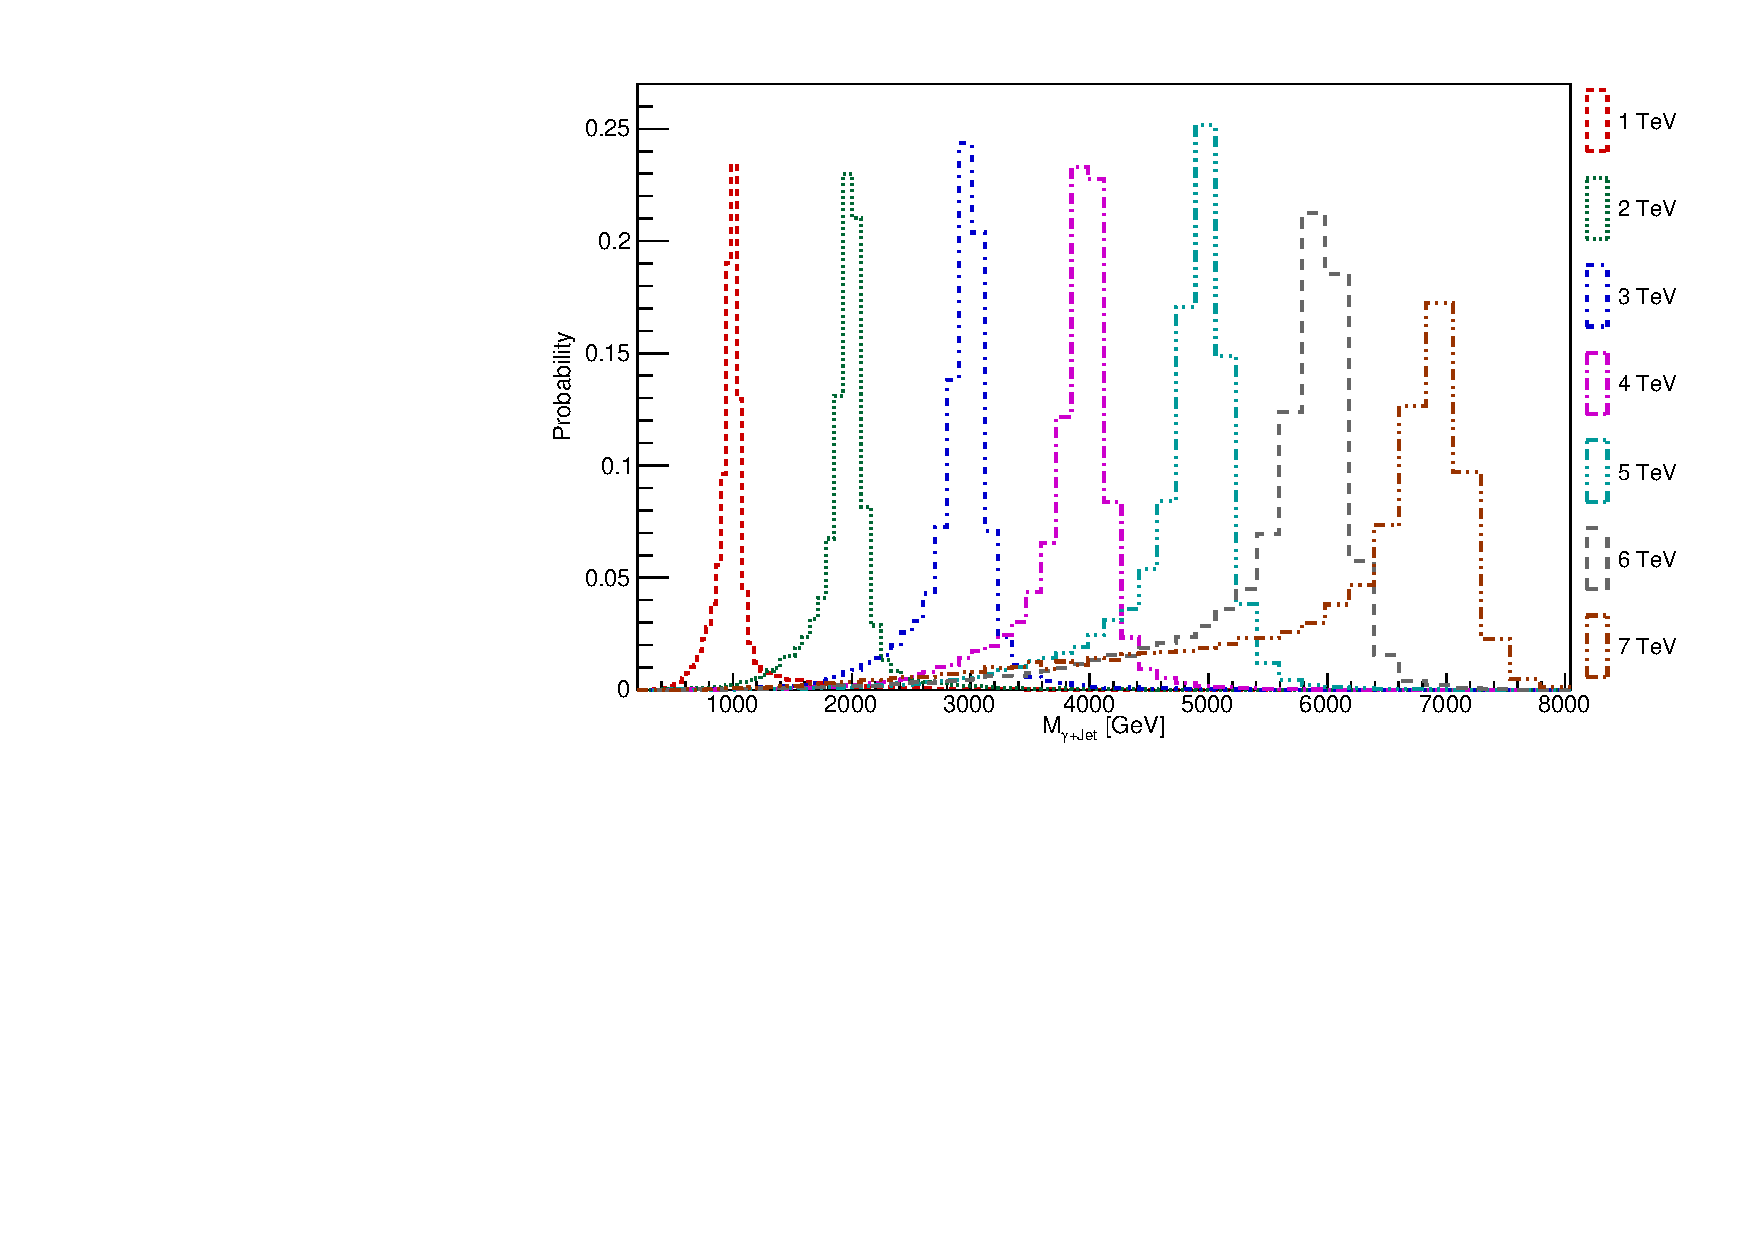
\includegraphics[width=7.9cm]{Chapter4/SignalShapes/SigShapes_Qstar_f1p0.pdf}} 
 \subfloat[\bstar, $f = 1.0$]{\label{}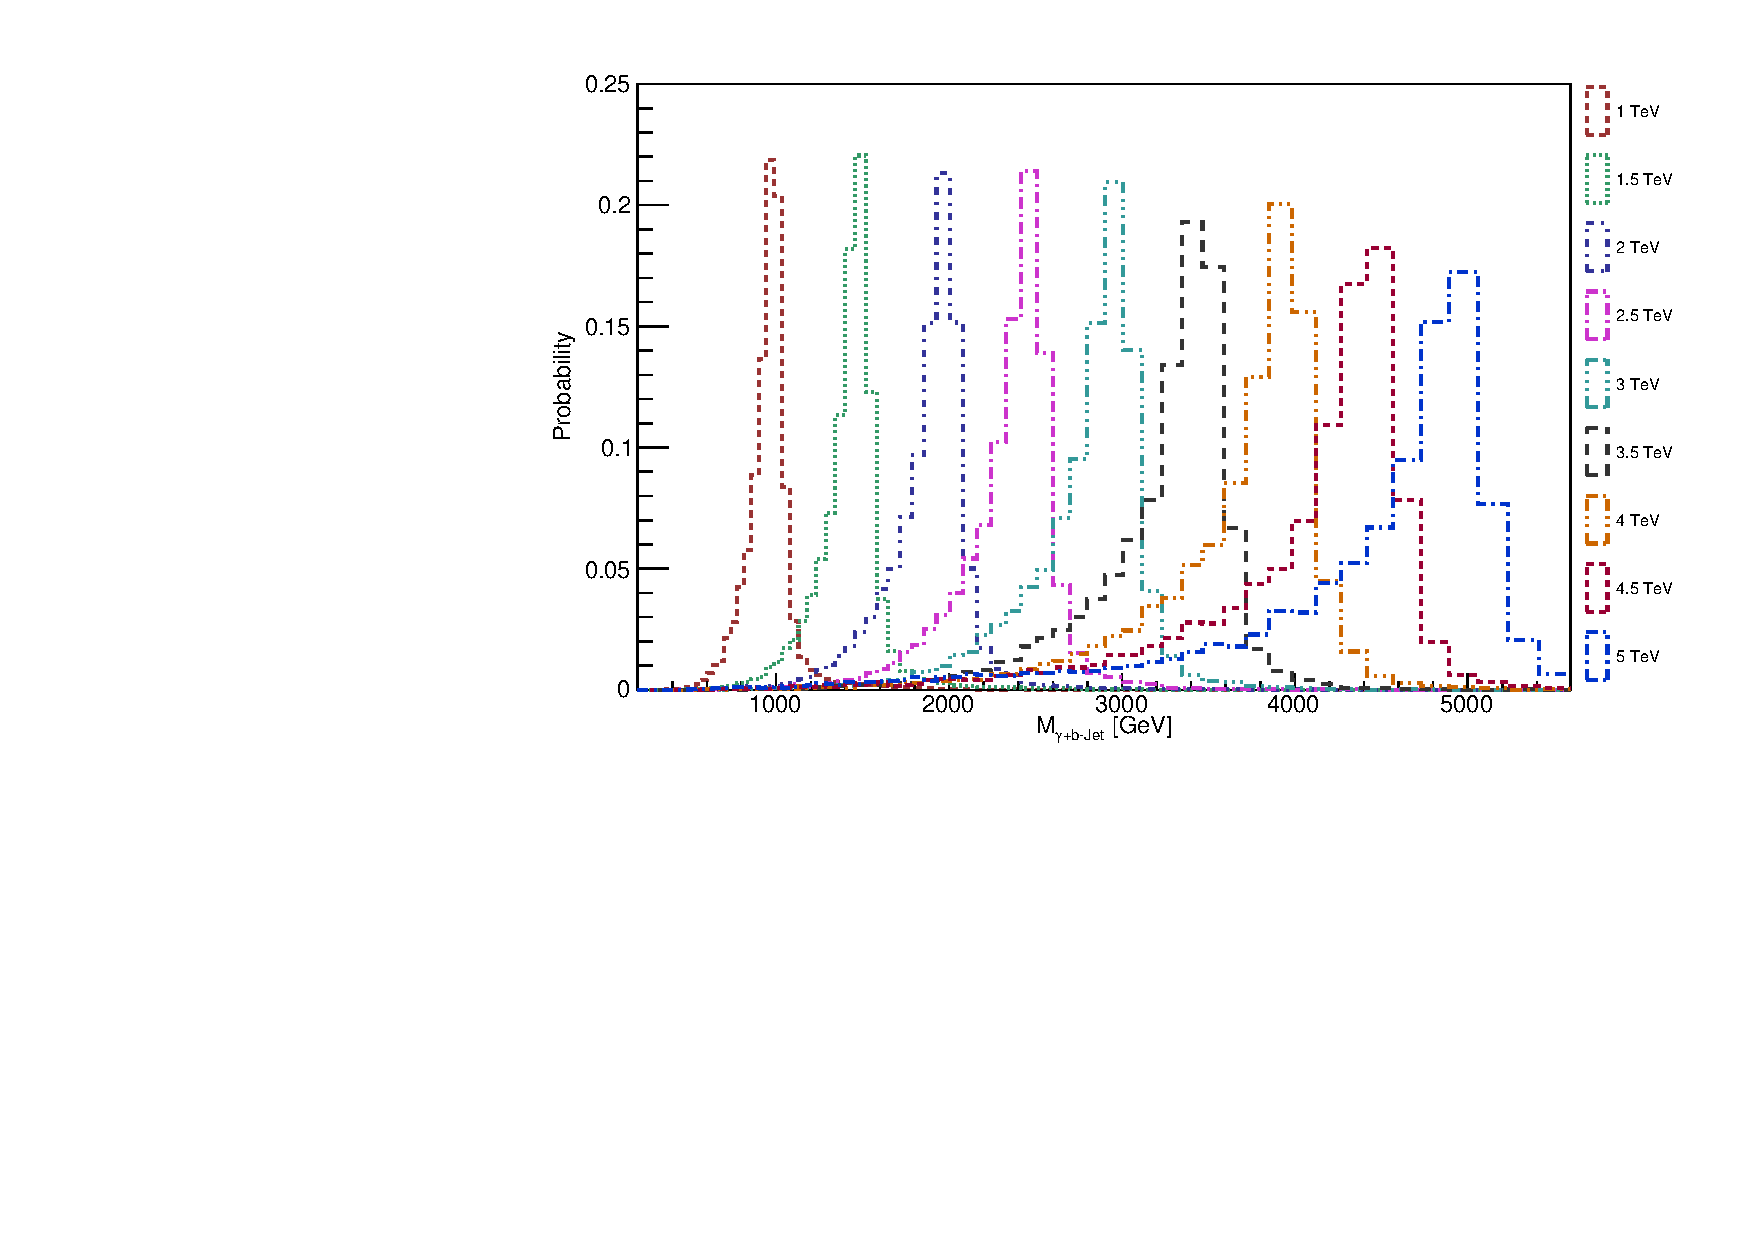
\includegraphics[width=7.9cm]{Chapter4/SignalShapes/SigShapes_Bstar_f1p0_1tag.pdf}}\\
 \subfloat[\qstar, $f = 0.5$]{\label{}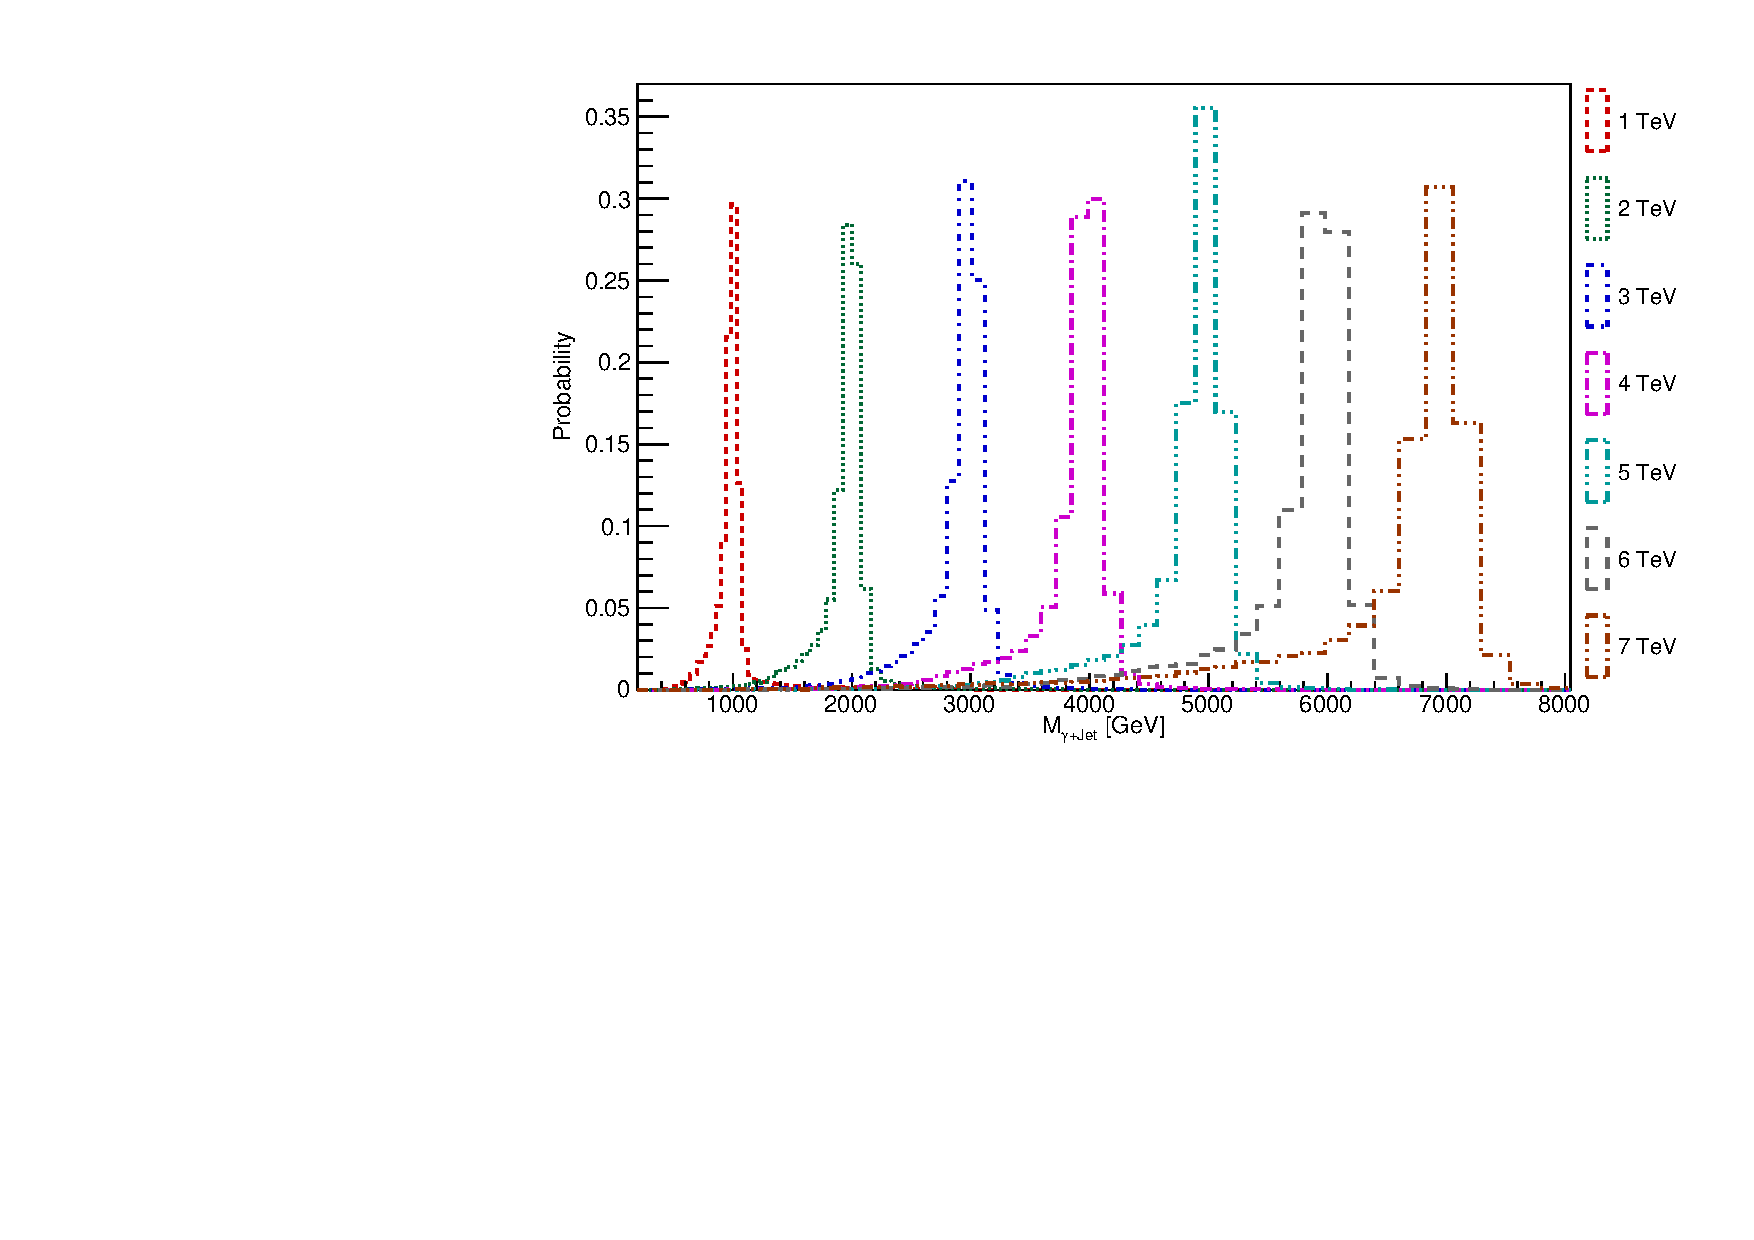
\includegraphics[width=7.9cm]{Chapter4/SignalShapes/SigShapes_Qstar_f0p5.pdf}}
 \subfloat[\bstar, $f = 0.5$]{\label{}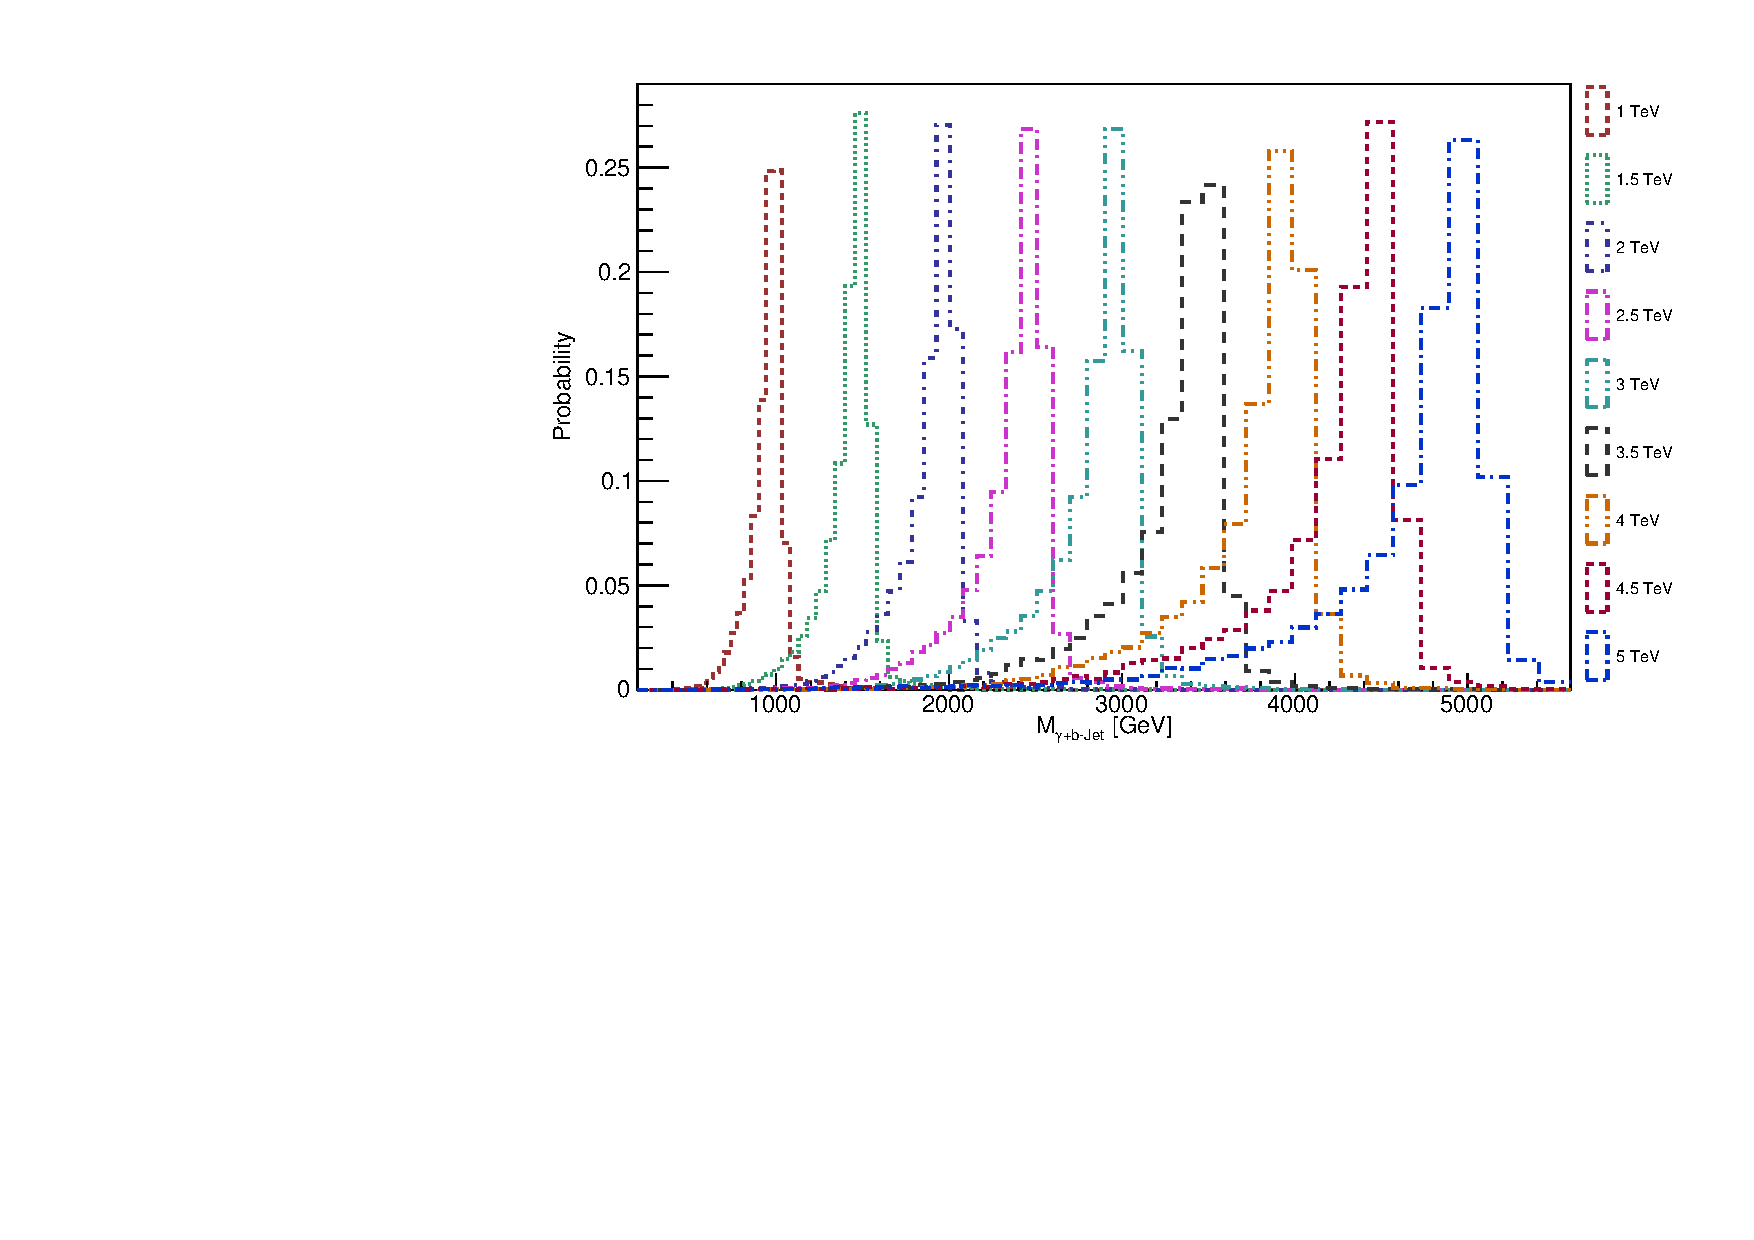
\includegraphics[width=7.9cm]{Chapter4/SignalShapes/SigShapes_Bstar_f0p5_1tag.pdf}}\\
 \subfloat[\qstar, $f = 0.1$]{\label{}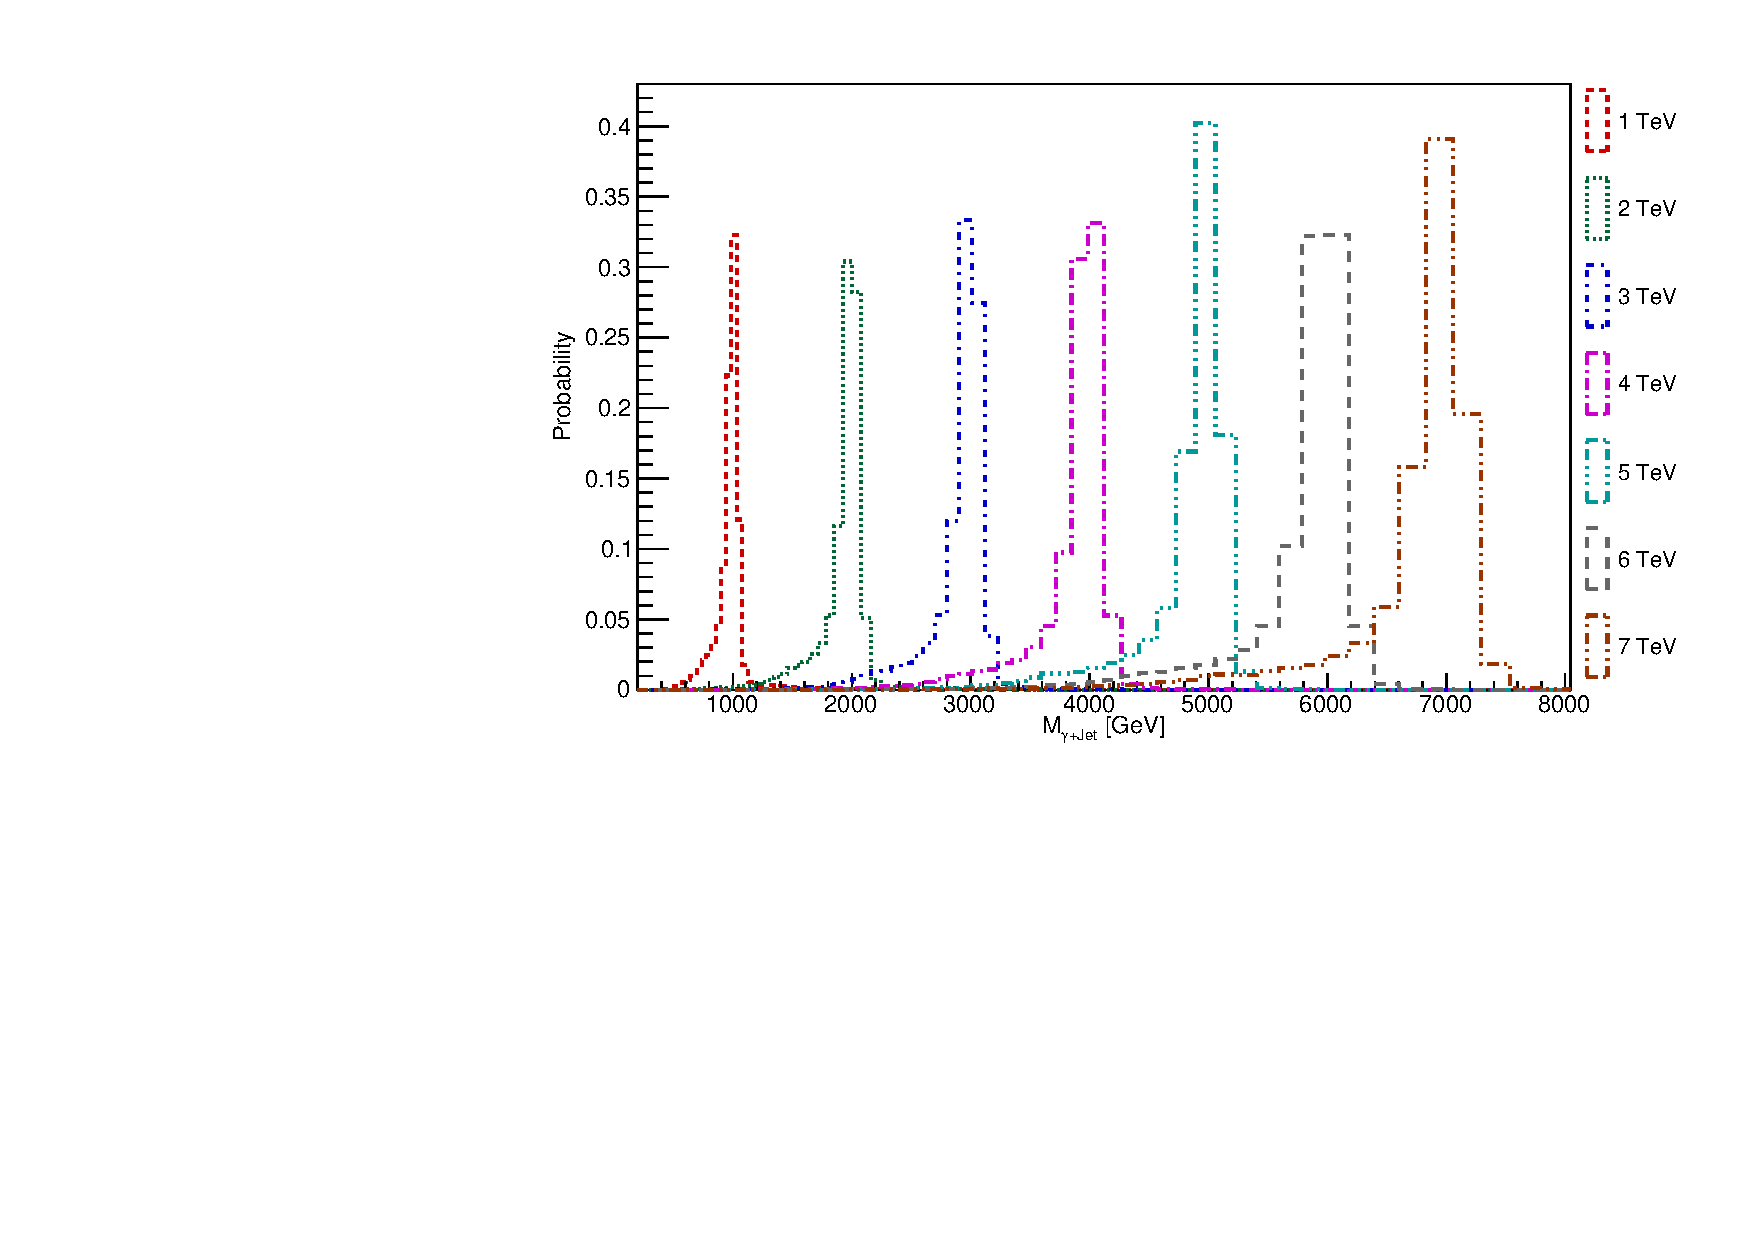
\includegraphics[width=7.9cm]{Chapter4/SignalShapes/SigShapes_Qstar_f0p1.pdf}}
 \subfloat[\bstar, $f = 0.1$]{\label{}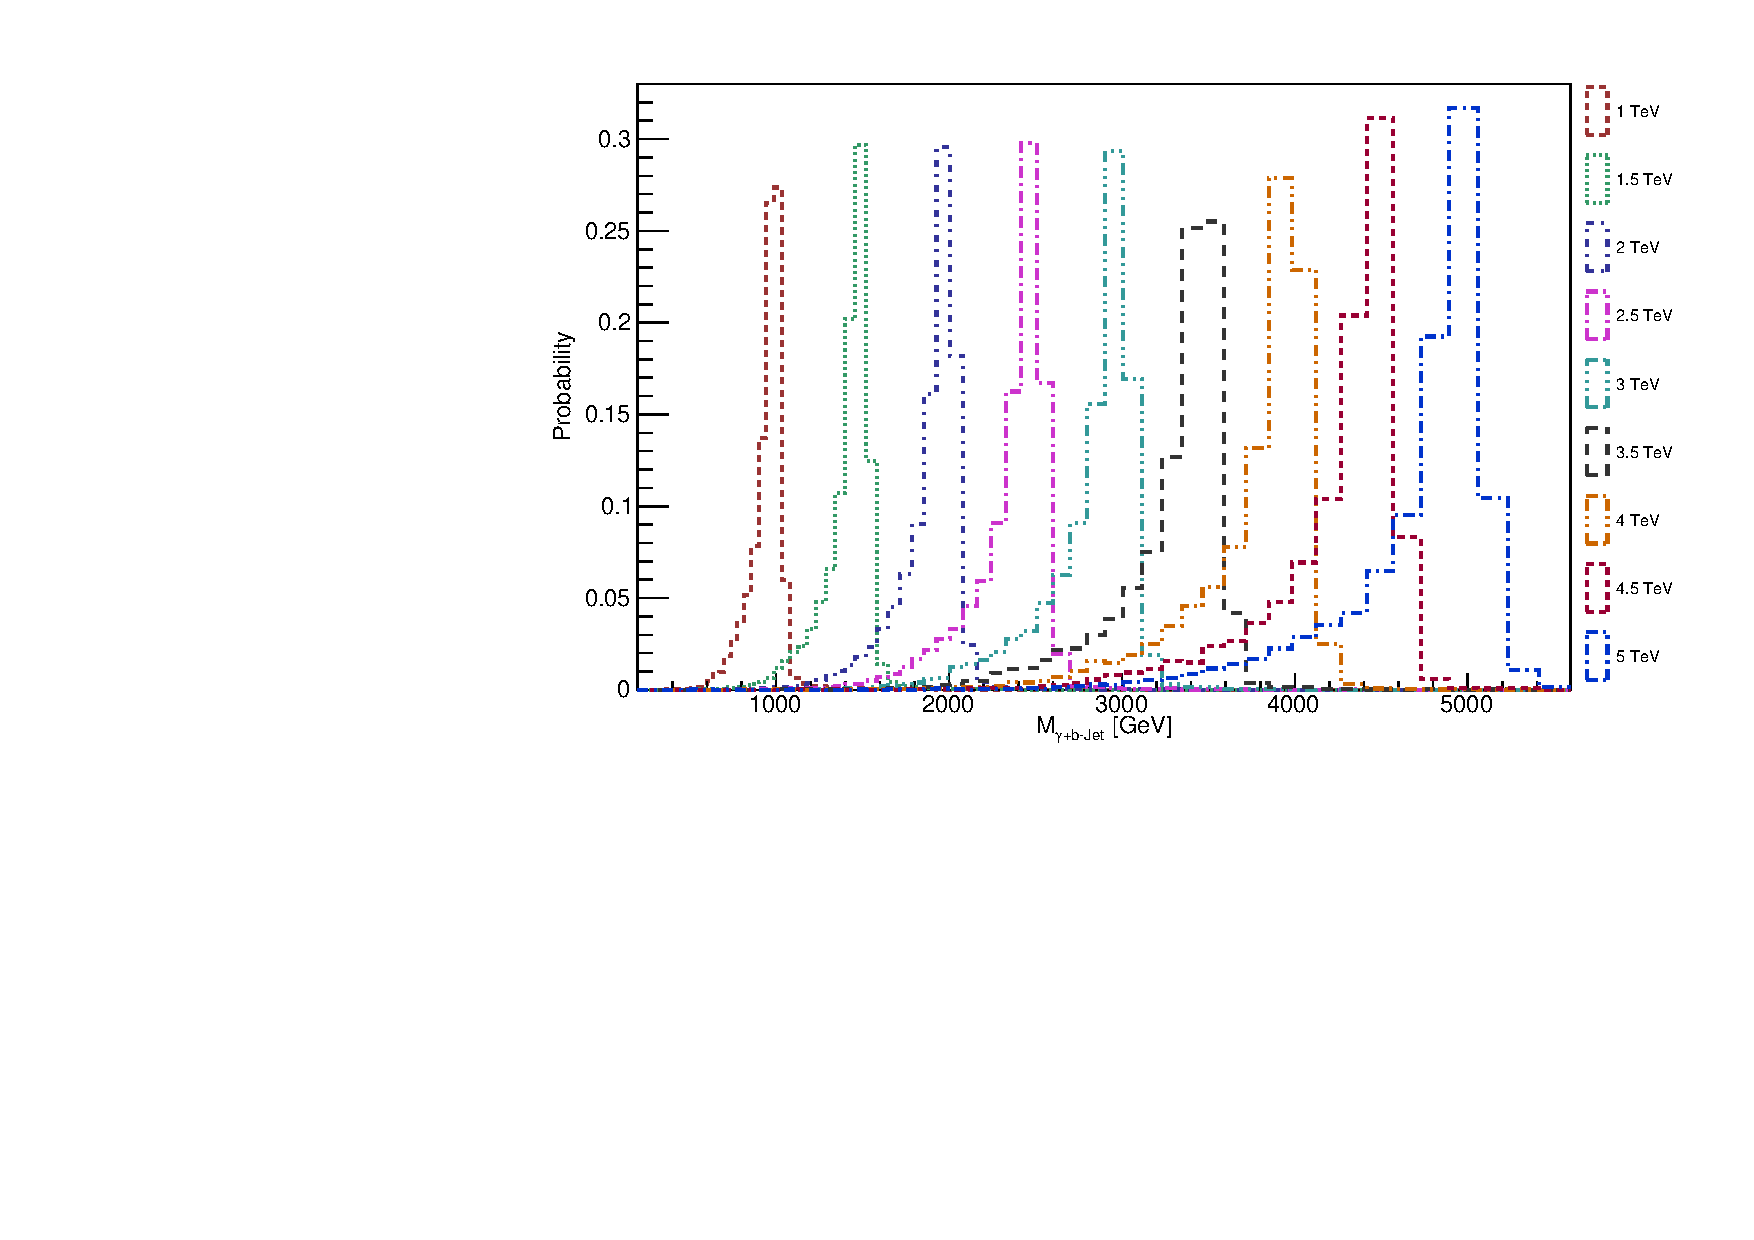
\includegraphics[width=7.9cm]{Chapter4/SignalShapes/SigShapes_Bstar_f0p1_1tag.pdf}} 
 \caption{Signal shapes for \qstar (left) and \bstar (right) for different masses and couplings.}
\label{fig:SigShapes}
\end{figure}

\subsubsection{Background MC}
The list of MC samples, along with the number of generated events and process cross-section,
corresponding to the three backgrounds for this study are presented in \tab{\ref{Table:BkgSamples}} below.
%---------------TABLE FOR MC samples-------------------
\begin{table}[h!]
  \begin{center}
    \resizebox{16cm}{!}{
      \begin{tabular}{lcc}
        \toprule
        \belowrulesepcolor{Mygray}
        \belowrulesepcolor{Mygray}
        \belowrulesepcolor{Mygray}
        \rowcolor{Mygray}[\dimexpr\tabcolsep+0.09pt\relax]
        \bf {Sample Name} & \bf {Events}  & \bf{Cross section (in $\unit{pb}$)} \\
        \aboverulesepcolor{Mygray}
        \aboverulesepcolor{Mygray}
        \aboverulesepcolor{Mygray}
        \midrule
        GJets\_HT-40To100\_TuneCUETP8M1\_13TeV-madgraphMLM-pythia8   & 4,467,985  & 20820 \\
        GJets\_HT-100To200\_TuneCUETP8M1\_13TeV-madgraphMLM-pythia8  & 5,131,873  & 9201  \\
        GJets\_HT-200To400\_TuneCUETP8M1\_13TeV-madgraphMLM-pythia8  & 10,036,487 & 2308  \\
        GJets\_HT-400To600\_TuneCUETP8M1\_13TeV-madgraphMLM-pythia8  & 2,529,729  & 275.2 \\
        GJets\_HT-600ToInf\_TuneCUETP8M1\_13TeV-madgraphMLM-pythia8  & 2,463,946  & 93.3  \\
        \midrule
        \midrule
        QCD\_Pt\_120to170\_TuneCUETP8M1\_13TeV\_pythia8    & 6,708,572 & 471100      \\
        QCD\_Pt\_170to300\_TuneCUETP8M1\_13TeV\_pythia8    & 6,958,708 & 117276      \\
        QCD\_Pt\_300to470\_TuneCUETP8M1\_13TeV\_pythia8    & 4,150,588 & 7823        \\
        QCD\_Pt\_470to600\_TuneCUETP8M1\_13TeV\_pythia8    & 3,959,986 & 648.2       \\
        QCD\_Pt\_600to800\_TuneCUETP8M1\_13TeV\_pythia8    & 3,896,412 & 186.9       \\
        QCD\_Pt\_800to1000\_TuneCUETP8M1\_13TeV\_pythia8   & 3,992,112 & 32.29      \\
        QCD\_Pt\_1000to1400\_TuneCUETP8M1\_13TeV\_pythia8  & 2,999,069 & 9.418      \\
        QCD\_Pt\_1400to1800\_TuneCUETP8M1\_13TeV\_pythia8  & 396,409   & 8.426E$-$1     \\
        QCD\_Pt\_1800to2400\_TuneCUETP8M1\_13TeV\_pythia8  & 397,660   & 1.149E$-$1    \\
        QCD\_Pt\_2400to3200\_TuneCUETP8M1\_13TeV\_pythia8  & 399,226   & 6.830E$-$3  \\
        QCD\_Pt\_3200toInf\_TuneCUETP8M1\_13TeV\_pythia8   & 391,735   & 1.654E$-$4 \\
        \midrule
        \midrule
        DYJetsToLL\_Pt-100To250\_TuneCUETP8M1\_13TeV-amcatnloFXFX-pythia8  & 2,040,596 & 83.12  \\
        DYJetsToLL\_Pt-250To400\_TuneCUETP8M1\_13TeV-amcatnloFXFX-pythia8  & 423,976   & 3.047  \\
        DYJetsToLL\_Pt-400To650\_TuneCUETP8M1\_13TeV-amcatnloFXFX-pythia8  & 432,056   & 3.921E$-$1 \\
        DYJetsToLL\_Pt-650ToInf\_TuneCUETP8M1\_13TeV-amcatnloFXFX-pythia8  & 430,691   & 3.636E$-$2\\
        WJetsToLNu\_TuneCUETP8M1\_13TeV-madgraphMLM-pythia8 & 29,705,748 & 61526.7  \\
        \bottomrule
      \end{tabular}
    }
    \caption{The background MC samples used in this analysis, simulated and reconstructed at $\sqrt{s}$ = 13 TeV.}
    \label{Table:BkgSamples}
  \end{center}
\end{table}


\vspace{-0.3in}

The SM $\gamjet$ background has been generated using the \MGvATNLO 2.2.2~\cite{Alwall:2014hca} event generator in different H$_{\textrm{T}}$\footnote{H$_{\textrm{T}}$ =
  $\sum{\pt}$ of all the jets in an event} bins, in the range of $40-100$, $100-200$, $200-400$, $400-600$ and $600-\infty$\unit{GeV} with showering and hadronization
carried out by the \pythia program. The MLM~\cite{Alwall:2007fs} matching scheme has been used to remove the double counting of the partons generated with
\madgraph and \pythia.    

The SM QCD dijet background has been generated using \pythia, with the same conditions as signal MC, in different \pt bins, in the range of
$120-170$, $170-300$, $300-470$, $470-600$, $600-800$, $800-1000$, $1000-1400$, $1400-1800$,
$1800-2400$, $2400-3200$ and $3200-\infty$\unit{GeV}.

The EWK Z$+$jet background has been generated in different \pt bins in the range of $100-250$, $250-400$, $400-650$ and $650-\infty$\unit{GeV}
using the \amcatnlo event generator with FXFX~\cite{Alwall:2007fs} matching scheme
and \pythia for showering and hadronization. The corresponding W$+$jet background is generated using the \madgraph event generator
with MLM matching scheme and \pythia for showering and hadronization. All the samples use CUETP8M1 as the underlying event tune.

\section{Re-weighting of MC events}
The detector data is compared with the MC samples to validate it w.r.t.\ the theoretical description. In order to have a fair comparison, both data and MC
are kept at equal footing, by weighting the MC events corresponding to the data.
\subsection{Luminosity re-weighting}
The MC events are re-weighted to reflect the data luminosity. The relevant luminosity weight per event applied to MC is:
\begin{equation}
w_{\textrm{lumi}} = \frac{\sigma_{\textrm{process}} \times \mathcal{L}_{\textrm{data}}}{\textrm{N}_{\textrm{process}}}
\end{equation}
where $\sigma_{\textrm{process}}$ and $\textrm{N}_{\textrm{process}}$ are the theoretical cross-section and the number of generated events for the simulated
process and $\mathcal{L}_{\textrm{data}}$ is the total integrated luminosity of data.
\subsection{Pile-up re-weighting}
In high-luminosity colliders, each bunch crossing may result into many inelastic interactions, with the number of interactions being proportional to the
instantaneous luminosity of the collision. These additional interactions are attributed to as the pile-up (PU) interactions. These pile-up events can
affect the reconstruction efficiency and can appear in the \pt distribution of the reconstructed objects. 
The presence of pile-up can affect the current analysis in two ways: additional energy from PU can be added to the reconstructed jet energy, thereby, worsening the jet
energy measurement and tracks and calorimeter energy deposits from PU interactions can get added to the isolation energy sum of photons, thereby, making the
isolation cuts less efficient. However, a number of techniques are developed and centrally validated in CMS to alleviate the deterioration of object
reconstruction due to PU effects. To minimize the impact of PU interactions, various cuts applied for object selection and energy corrections are optimized so that
in the end, the effect is almost negligible.

The simulated samples are also generated with additional pile-up to match with the actual data taking conditions. The samples used in this analysis are generated
with 2015\_25ns\_Startup\_PoissonOOTPU~\cite{Web:PileupScenario} pile-up scenario. Still, the residual differences in the pile-up distributions of data and MC are 
corrected by means of pile-up re-weighting. In this process, the pileup distribution for data is taken from the instantaneous luminosity per bunch
crossing for each luminosity section, and the total pp inelastic cross-section of 69.2\unit{mb}, using the officially recommended procedure~\cite{Web:PileupScenario}.
A Poissonian smearing is used to model the statistical fluctuations in the actual pileup events present in the data. For MC, the true number of
interactions per event are considered as the pileup distribution. These pile-up distributions in data and MC are compared corresponding to the number
of primary vertices and a weight factor is calculated on the event by event basis. This weight factor is then multiplied to the luminosity weight factor to
get the total event weight applied to the Monte Carlo events. To give an account of the effect, a data-MC comparison of
the number of vertices in an event has been shown in \fig{\ref{fig:PUrewt}}, before
and after applying the pile-up re-weighting.
\begin{figure}[h!]
\centering
 \subfloat[Without PU weight]{\label{}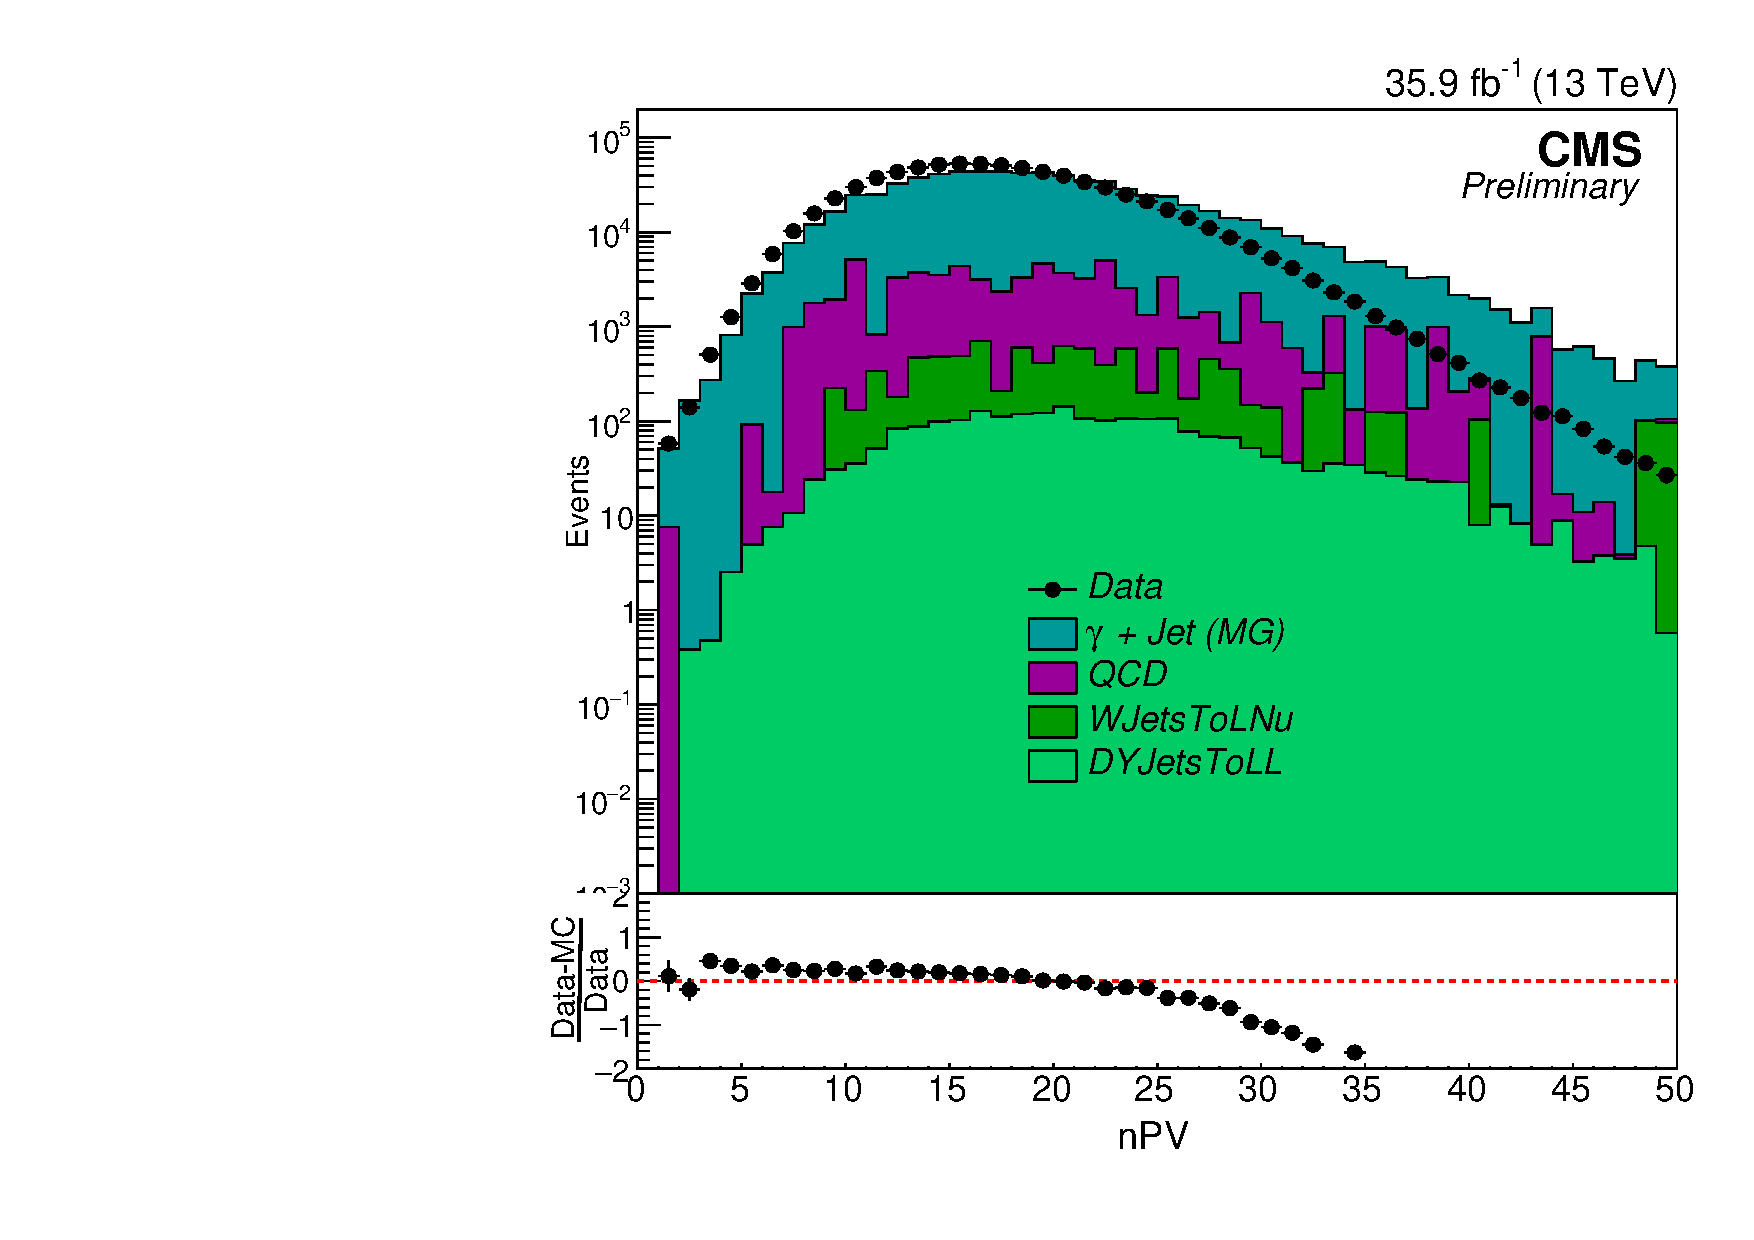
\includegraphics[width=8cm]{Chapter4/Pileup_rewt/Pileup_noPUWt.pdf}} 
 \subfloat[With PU weight]{\label{}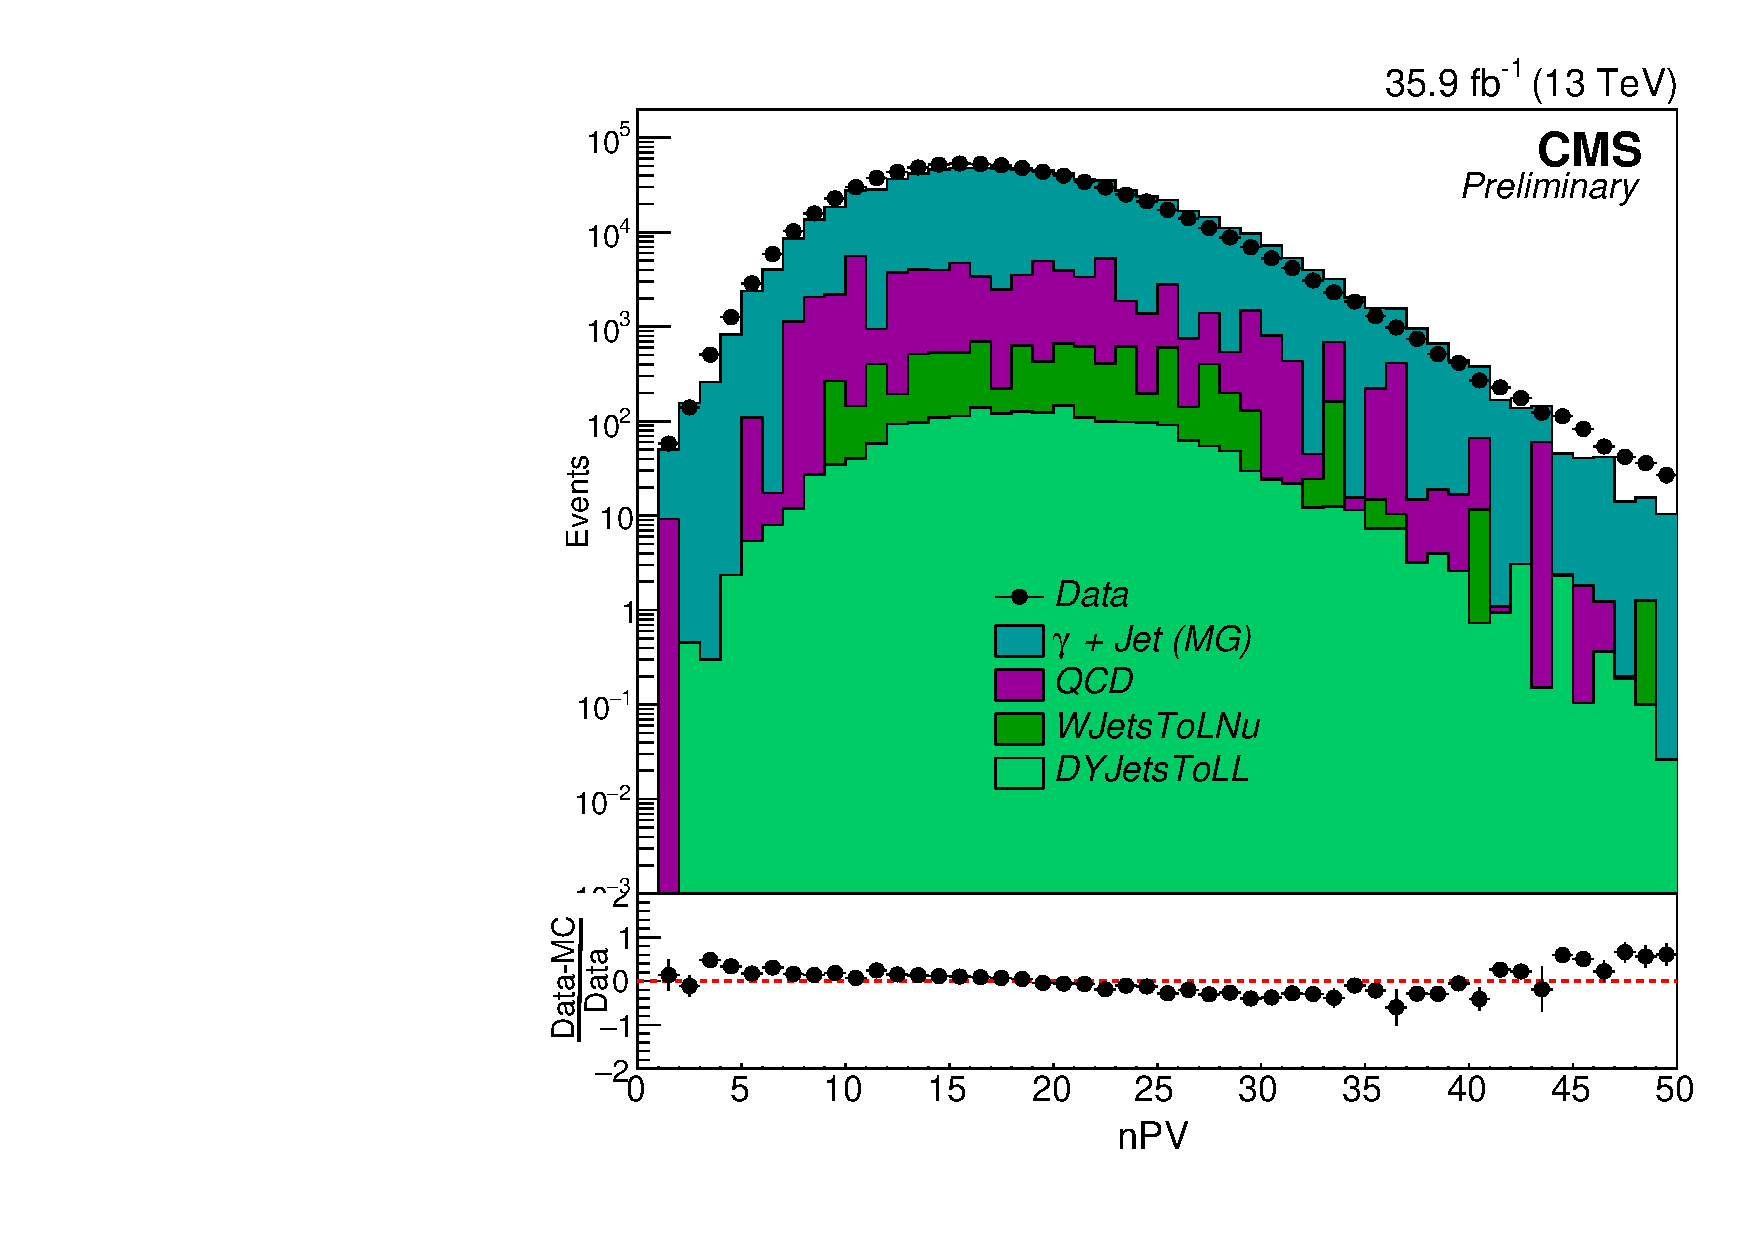
\includegraphics[width=8cm]{Chapter4/Pileup_rewt/Pileup_withPUWt.pdf}}
 \caption{Data-MC comparison of the number of vertices in an event, showing the effect of pile-up re-weighting.}
\label{fig:PUrewt}
\end{figure}
\vspace{-0.3in}
\section{Event selection}
In this analysis, we are searching for the possible signatures of excited quarks decaying into a photon and a jet final state. So the experimental technique of
event selection starts with the measurement of the inclusive process, pp $\rightarrow$ $\gamjet$ $+$ X where we require at least one hard photon and one hard jet
in the event, X refers to the additional photons or jets or anything else that can be present in the event. The events containing these additional particles are
not vetoed as it would unnecessarily restrict our signal to a narrow topology. The event statistics for the search of excited b-quark is formed by requiring the selected
jet to be a b-jet. Based on the type of the jet, three different event categories are made:
\vspace{-0.1in}
\begin{itemize}[leftmargin=*]
\item {\bf{Inclusive category}}: Events containing photons and jets where jets can be the light jets or the b-jets. This forms the event statistics for \qstar
  search.
\item {\bf{Exclusive 1 b-tag category}}: Events containing photons and b-jets, forming the event statistics for \bstar search.
\item {\bf{Exclusive 0 b-tag category}}: Events containing photons and non b-jets. This category is also used in \bstar search in order to overcome
  any loss of statistical power due to migration of events from one category to another.
\end{itemize}
\vspace{-0.1in}
The selection criteria used in this analysis is described in detail in the sections below:
\subsection{Trigger selection}
The trigger system of the CMS experiment is designed to select interesting physics events of good quality. As mentioned in \sectn{\ref{Se:CMS_trigger}}, it
consists of two levels: the L1 trigger and the HLT trigger. The data sample used in this analysis is required to pass the L1\_SingleEG40 trigger, which
selects the events that have at least one $e/\gamma$ candidate with E$_{\textrm{T}}$ $>$ 40\unit{GeV} and HLT$\_$Photon165$\_$HE10 trigger, which is a single
photon trigger requiring the events to have at least one photon candidate with \pt $>$ 165\unit{GeV} and H$/$E fraction $<$ 10$\%$. The HLT path is
required to be un-prescaled for the entire data taking period, so that all events passing the trigger are stored for further analysis.

The offline trigger efficiency of HLT trigger, also referred to as the trigger turn-on, has been studied as a function of the leading photon \pt in order to
observe any inefficiencies. The trigger turn-on measured w.r.t.\ the same object dataset is referred to as the relative trigger efficiency while
the trigger turn-on measured w.r.t.\ an orthogonal dataset is referred to as the absolute trigger efficiency, as the relative trigger efficiency can not reveal the
presence of any systematic detector effect. The idea is to identify unbiased photon candidates in data and measure the frequency of photons activating
the trigger decision. The trigger efficiency in this analysis has been evaluated w.r.t.\ the lower \pt prescaled photon, jet and muon reference triggers, as listed
in \tab{\ref{Table:trigturnon}}. This efficiency is measured by selecting the events passing the lower \pt threshold triggers and computing the rate at which
these events also pass the main analysis trigger. The trigger turn-on curve for all the three reference triggers is presented in \fig{\ref{fig:TrigTurnOn}}.

\vspace{0.12in}
%---------------TABLE FOR TRIGGER TURN ON of EXCITED QUARK AND b-QUARK-------------------
\begin{table}[h]
  \begin{center}
    \resizebox{15cm}{!}{
      \begin{tabular}{cccc}
        \toprule
        \belowrulesepcolor{Mygray}
        \belowrulesepcolor{Mygray}
        \belowrulesepcolor{Mygray}
        \rowcolor{Mygray}[\dimexpr\tabcolsep+0.09pt\relax]
        \bf {Analysis trigger}  &  \bf {Photon ref.\ triggers } & \bf {Jet ref.\ triggers} & \bf {Muon ref.\ triggers} \\
        \aboverulesepcolor{Mygray}
        \aboverulesepcolor{Mygray}
        \aboverulesepcolor{Mygray}
        \midrule
        HLT\_Photon165\_HE10 &  HLT\_Photon75 & HLT\_PFJet60  & HLT\_Mu50 \\
        & HLT\_Photon90 &  HLT\_PFJet80  & \\ 
        &  HLT\_Photon120 & HLT\_PFJet140 & \\
        \bottomrule
      \end{tabular}
    }
    \caption{Different triggers used in the trigger efficiency study.}
    \label{Table:trigturnon}
  \end{center}
\end{table}



\vspace{-0.2in}
\begin{figure}[h!]
\centering
 \subfloat[Rel. Efficiency]{\label{}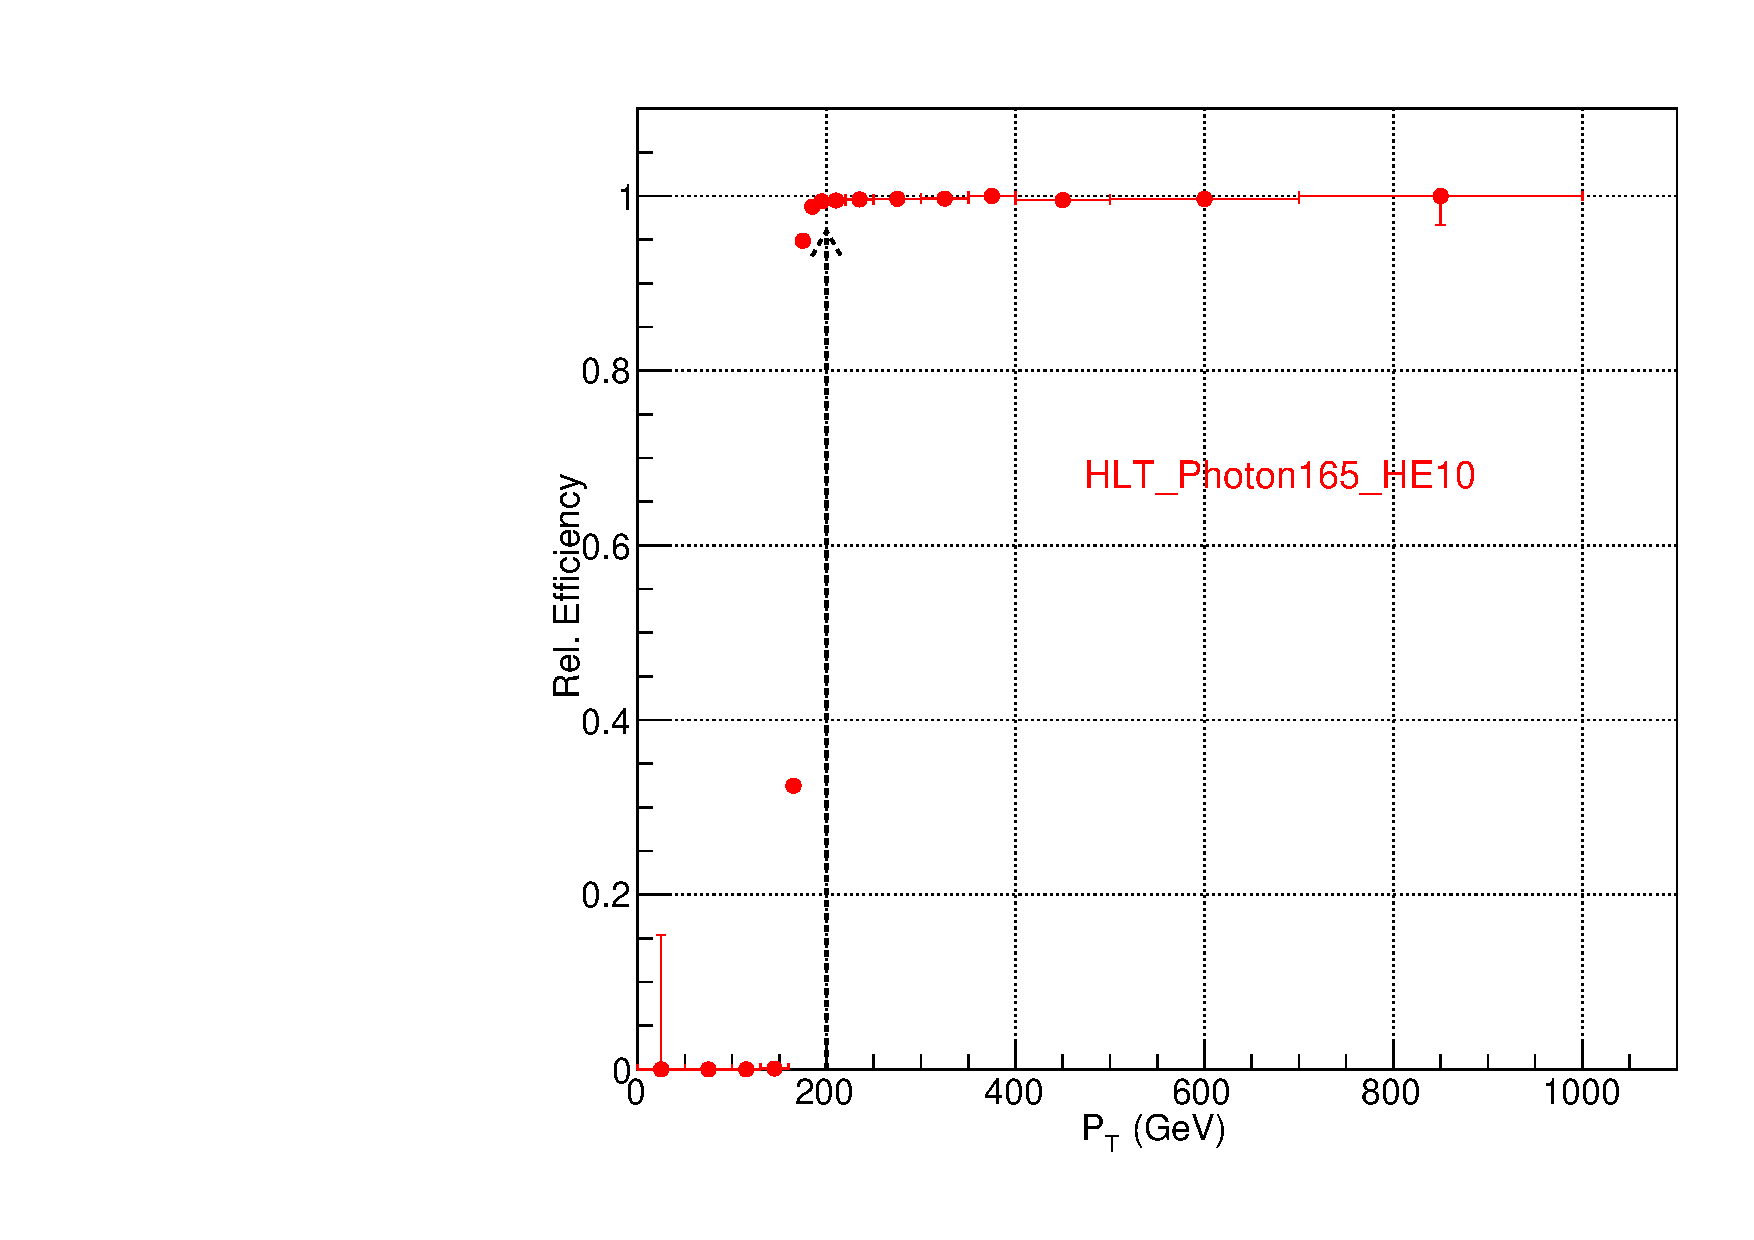
\includegraphics[width=5.3cm]{Chapter4/TriggerTurnOn/RelEff_PhtrigMatch_PhMID_EB.pdf}} 
 \subfloat[Abs. Efficiency (JetHT)]{\label{}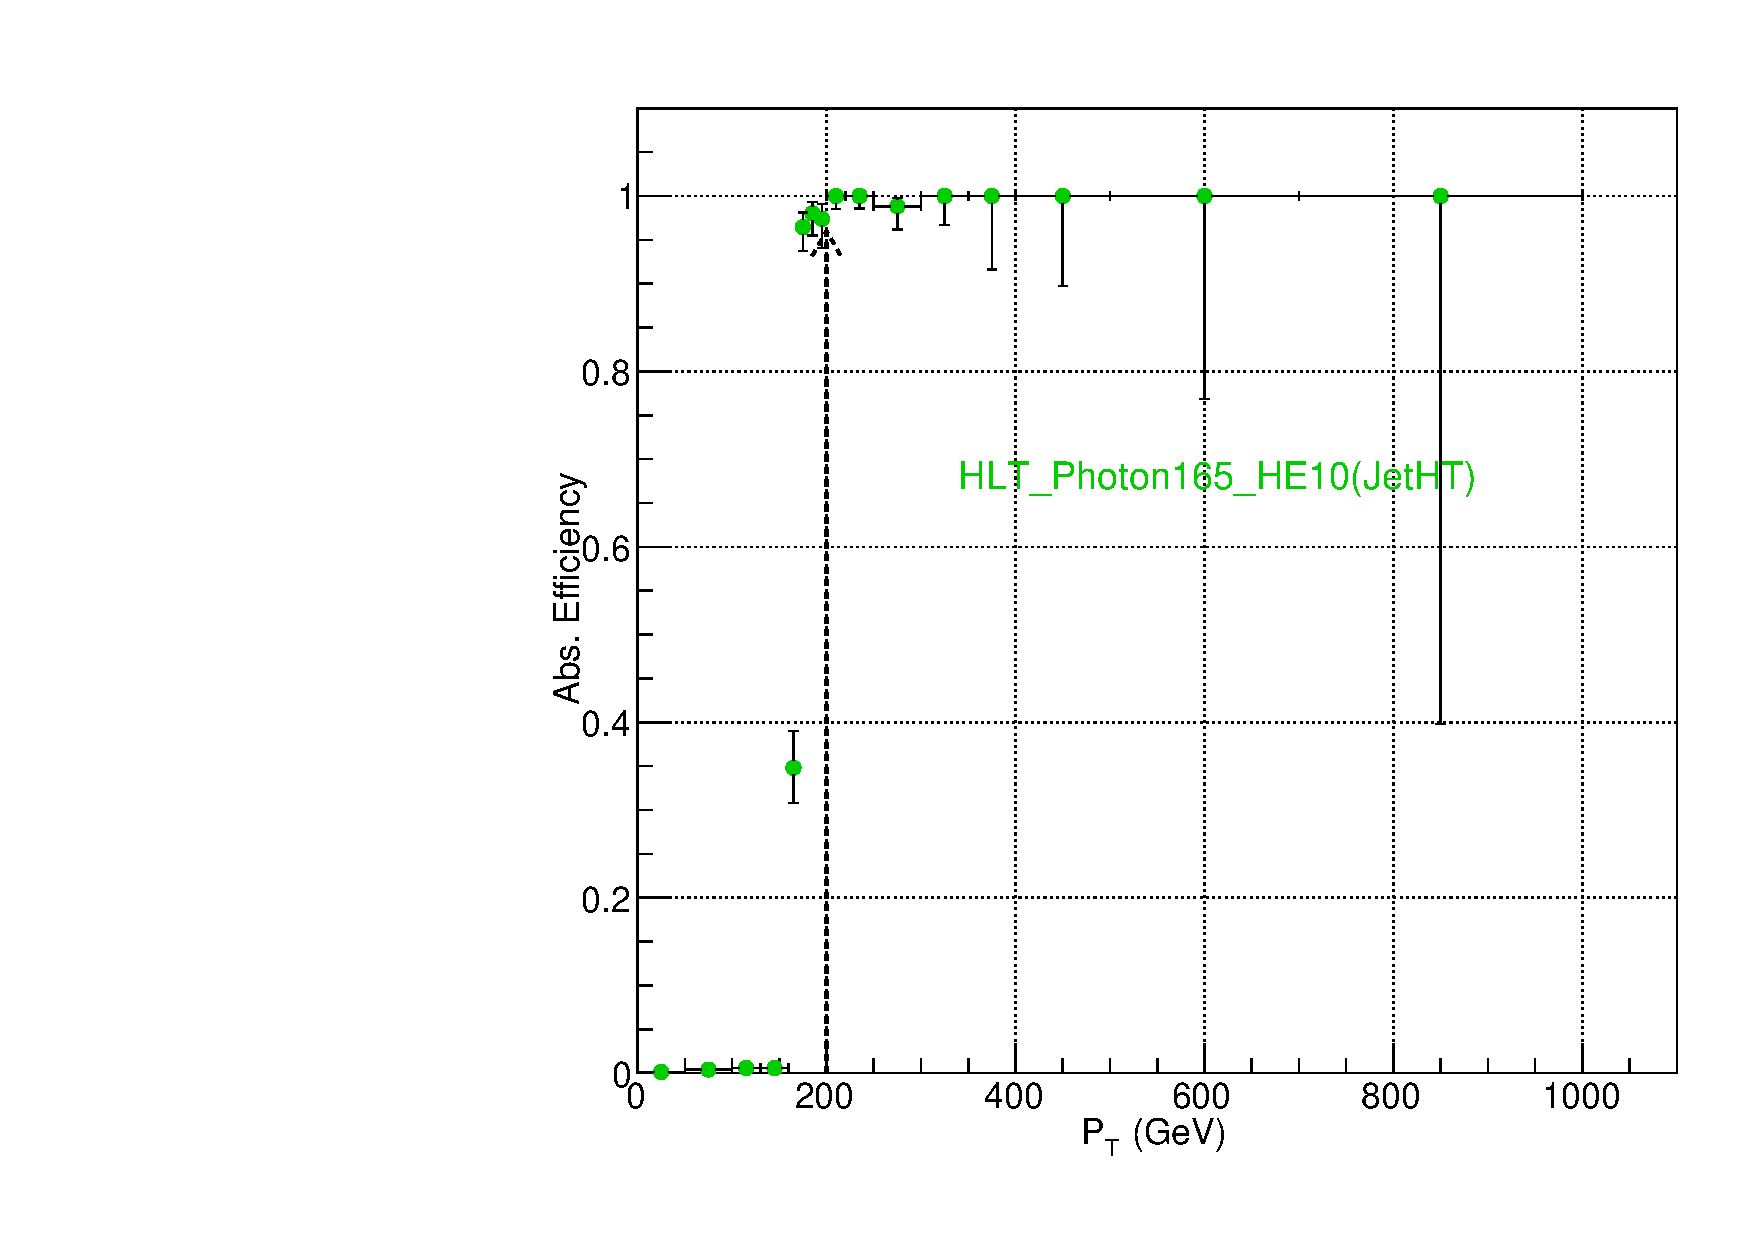
\includegraphics[width=5.3cm]{Chapter4/TriggerTurnOn/AbsEff_JetHT_JetObjMatch_PhMID_EB.pdf}}
 \subfloat[Abs. Efficiency (Muon)]{\label{}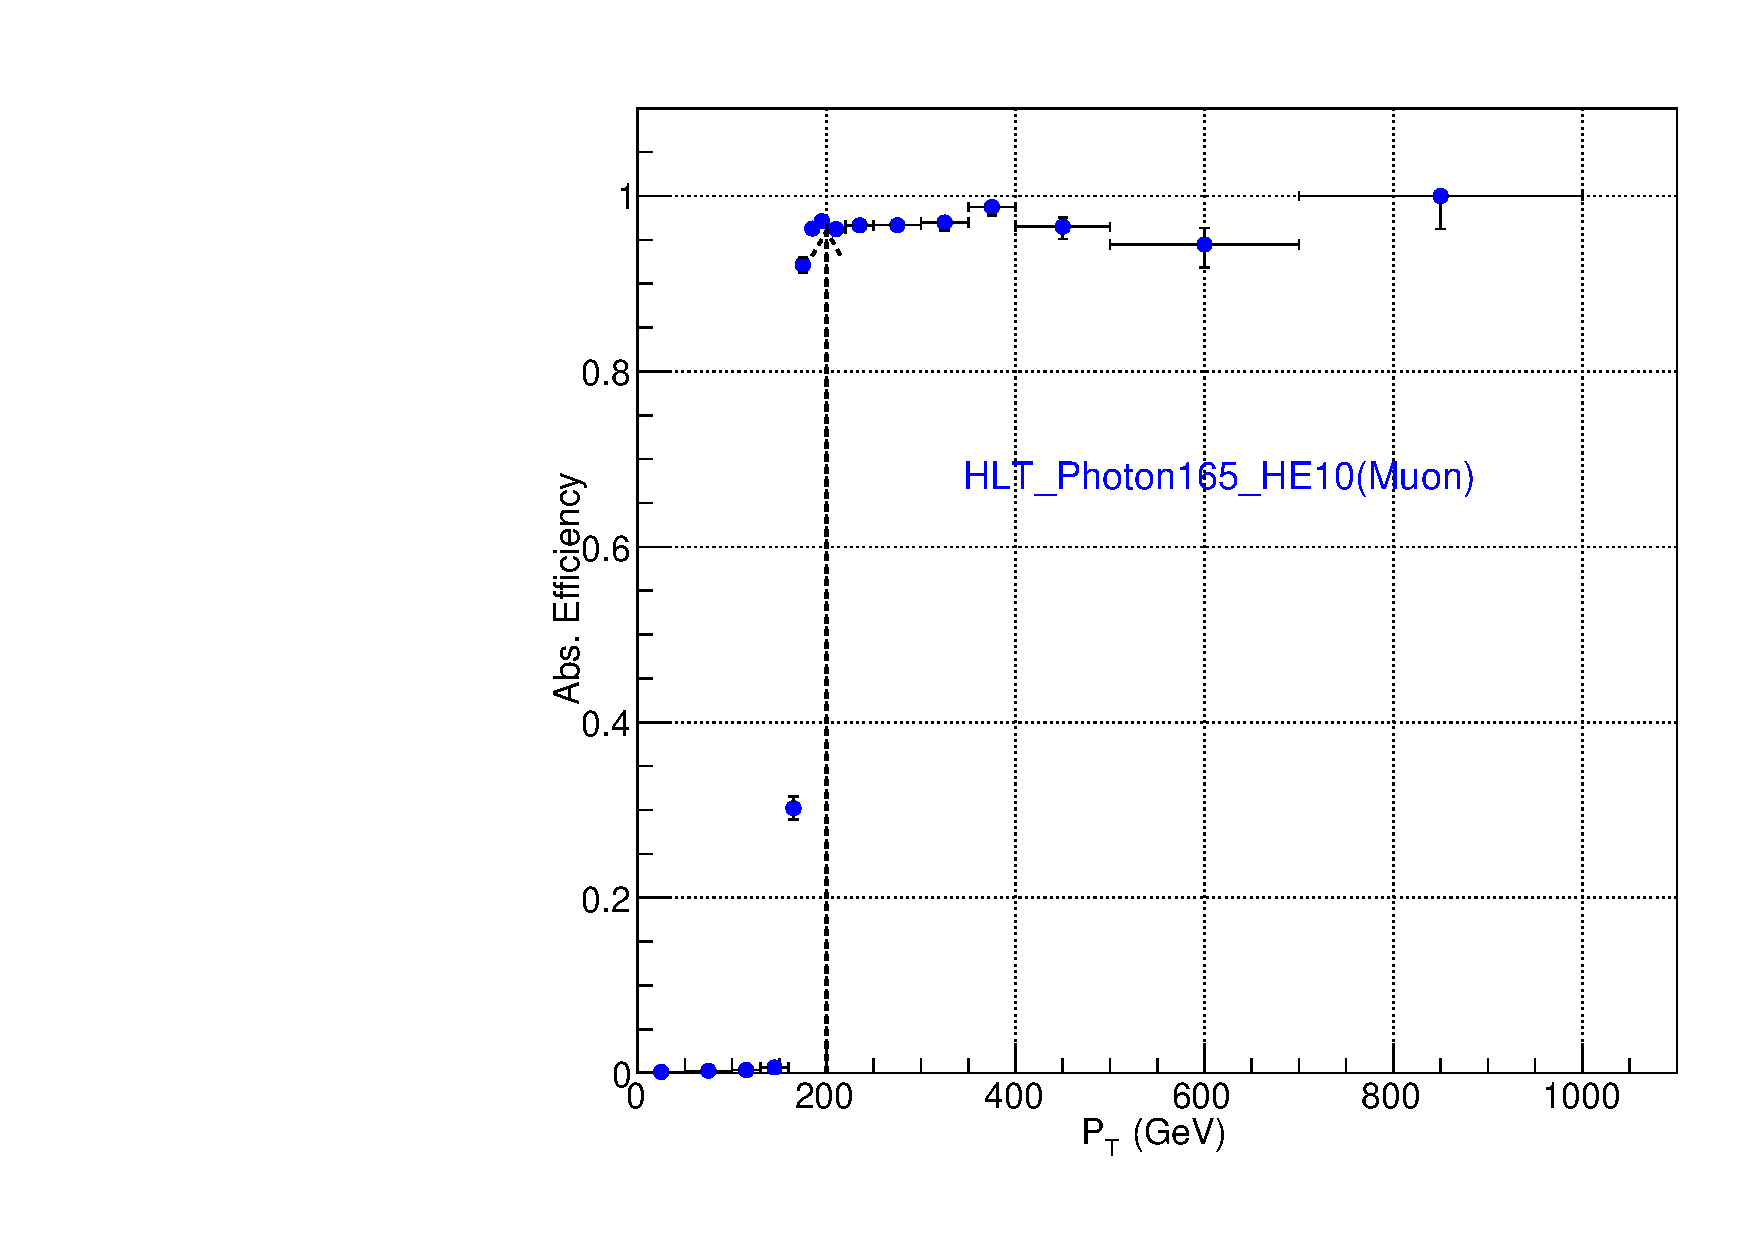
\includegraphics[width=5.3cm]{Chapter4/TriggerTurnOn/AbsEff_Mu_PhMID_EB.pdf}}
 \caption{Relative and absolute trigger efficiencies for the single photon trigger, HLT\_Photon165\_HE10.}
 \label{fig:TrigTurnOn}
\end{figure}
%\vspace{-0.15in}

It can be seen that the trigger become fully efficient and reaches the plateau region at around 200\unit{GeV}, for photon and jet reference triggers.
However, the turn-on w.r.t.\ the muon reference trigger is found to be around 95$\%$ efficient with
a sizable uncertainty which is taken into account as a systematic uncertainty.

\subsection{MET filters}
While monitoring the quality of detector data during offline processing, a number of noisy events were reported, which are removed by applying a set
of officially recommended noise cleaning filters, listed below:
\begin{itemize}[leftmargin=*]
\item {\bf{CSC tight beam halo filter}}: rejects muons from beam halo.
\item {\bf{HBHE noise filter with isolated noise rejection}}: rejects noisy events in HCAL.
\item {\bf{HCAL laser filter}}: removes events that contains HCAL calibration laser firing within the collision bunch-crossing.
\item {\bf{ECAL dead cell trigger primitive filter}}: rejects events containing large missing energy coming from masked crystals.
\item {\bf{Bad EE supercrystal filter}}: removes events that contains two EE crystals with anomalously high energies.
\end{itemize}

\subsection{Primary vertex selection}
A typical pp collision event may contain more than one reconstructed primary vertex coming from in-time and out-of-time bunch crossings, pile-up events etc.
But, the events that have at least one primary vertex coming from in-time collision are kept for further study. These events are selected by requiring the
vertex to be within 24\unit{cm} of the nominal collision point along the z$-$direction and within 2\unit{cm} in the radial direction. The vertex should have
at least 4 associated tracks, along with the largest value of $\sum{\pt^{2}}$ of all the tracks and have a proper 3d vertex fit with the tracks. 

\subsection{Analysis object selection: Photon}
In each event passing the primary vertex selection, we search for a well identified and isolated photon candidate by using the criteria explained in
\sectn{\ref{Se:Ph_identi}}. The cut-off value used for each variable is listed below:
\begin{itemize}[leftmargin=*]
\item \sigmaIetaIeta\ $<$ 0.01022.
\item Single tower H$/$E $<$ 0.0396.
\item Conversion safe electron veto $=$ true.
\item PF charged hadron isolation $<$ 0.441.
\item PF neutral hadron isolation $<$ 2.725 $+$ 0.0148 $\times$ $\pt^{\gamma}$ $+$ 0.000017 $\times$ ${(\pt^{\gamma})}^{2}$.
\item PF photon isolation $<$ 2.571 $+$ 0.0047 $\times$ $\pt^{\gamma}$.
\end{itemize}

The photon isolation cone is susceptible to a diffuse background of soft particles coming from the underlying events or pile-up events. 
So the isolation variables are corrected for the presence of these additional interactions using the following relation:
\begin{equation}
  \textrm{Iso}^{\textrm{corrected}} = \textrm{max.}(\textrm{Iso}^{\textrm{original}} - \rho_{\textrm{event}} \times \textrm{A}_{\textrm{eff}}\hspace{0.05in},\hspace{0.05in} 0.0)
\end{equation}
where, $\rho_{\textrm{event}}$ is known as the energy density computed using the FastJet package~\cite{Cacciari2011ma} and is defined as the median
energy density per unit area corresponding to the particles associated with the pile-up vertices. This quantity gives a measure of the pile-up activity in the
event. The variable, $\textrm{A}_{\textrm{eff}}$ is the ratio of the slopes obtained from linear fitting of $\rho-\textrm{N}_{\textrm{vtx}}$ and
Isolation$-\textrm{N}_{\textrm{vtx}}$. The values of $\textrm{A}_{\textrm{eff}}$ for three isolations, in different $\eta$ regions covering barrel and endcaps,
are shown in \tab{\ref{Table:photonAeff}}.

\begin{table}[h]
  \begin{center}
    \resizebox{14cm}{!}{
      \begin{tabular}{lccc}
        \toprule
        \belowrulesepcolor{Mygray}
        \belowrulesepcolor{Mygray}
        \belowrulesepcolor{Mygray}
        \rowcolor{Mygray}[\dimexpr\tabcolsep+0.09pt\relax]
        \bf {$\eta$-bin} & \bf {EA charged hadrons} & \bf {EA neutral hadrons} & \bf {EA photons}\\
        \aboverulesepcolor{Mygray}
        \aboverulesepcolor{Mygray}
        \aboverulesepcolor{Mygray}
        \midrule
        $|\eta|$ $<$ 1.0 &          0.0360 &	0.0597 &	0.1210 \\
        1.0 $<$ $|\eta|$ $<$ 1.479 & 0.0377 &	0.0807 &	0.1107 \\
        1.479 $<$ $|\eta|$ $<$ 2.0  & 0.0306 &	0.0629 &	0.0699 \\
        2.0 $<$ $|\eta|$ $<$ 2.2 	&   0.0283 &	0.0197 &	0.1056 \\
        2.2 $<$ $|\eta|$ $<$ 2.3 	&   0.0254 &	0.0184 &	0.1457 \\
        2.3 $<$ $|\eta|$ $<$ 2.4 	&   0.0217 &	0.0284 &	0.1719 \\
        $|\eta|$ $>$ 2.4 	&   0.0167 &	0.0591 &	0.1998  \\
        \bottomrule
      \end{tabular}
    }
    \caption{Effective area for different photon isolations.}
    \label{Table:photonAeff}
  \end{center}
\end{table}
\vspace{-0.2in}


In order to avoid non-collision backgrounds coming from the anomalous calorimeteric signals resulting due to the direct ionization of Avalanche Photo-diodes (APDs)
by a highly ionizing particle such as a proton and depositing all the energy within a single ECAL crystal (known as ``spikes''), a minimal requirement
on the rectangular ratios and shower shape profiles, as mentioned below, are also placed:
\begin{itemize}[leftmargin=*]
\item R$_{9}$ $<$ 1.0.
\item \sigmaIetaIeta $>$ 0.001.
\item \sigmaIphiIphi $>$ 0.001.
\end{itemize}

This selection results into a collection of photons in each event, out of which, the highest \pt photon (known as leading photon) is selected and is required
to be greater than 200\unit{GeV}, the \pt value at which the trigger turn-on curve becomes 100$\%$ efficient. The selected photon is also required to be in the
central barrel region of the detector, that is, $|{\eta}|$ $<$ 1.4442. This requirement is placed since the \qstar or \bstar resonances (if exists), produced
via hard scattering, would decay mostly into back-to-back $\gamma$ and jet and are expected to be detected in the central region of the detector.  
A comparison of Data vs.\ MC for different photon variables, after the final selection, is presented in \fig{\ref{fig:PhIdnIso}}.

\begin{figure}[htbp]
\centering
 \subfloat[$\sigmaIetaIeta$]{\label{fig:Ph_sigIetaIeta}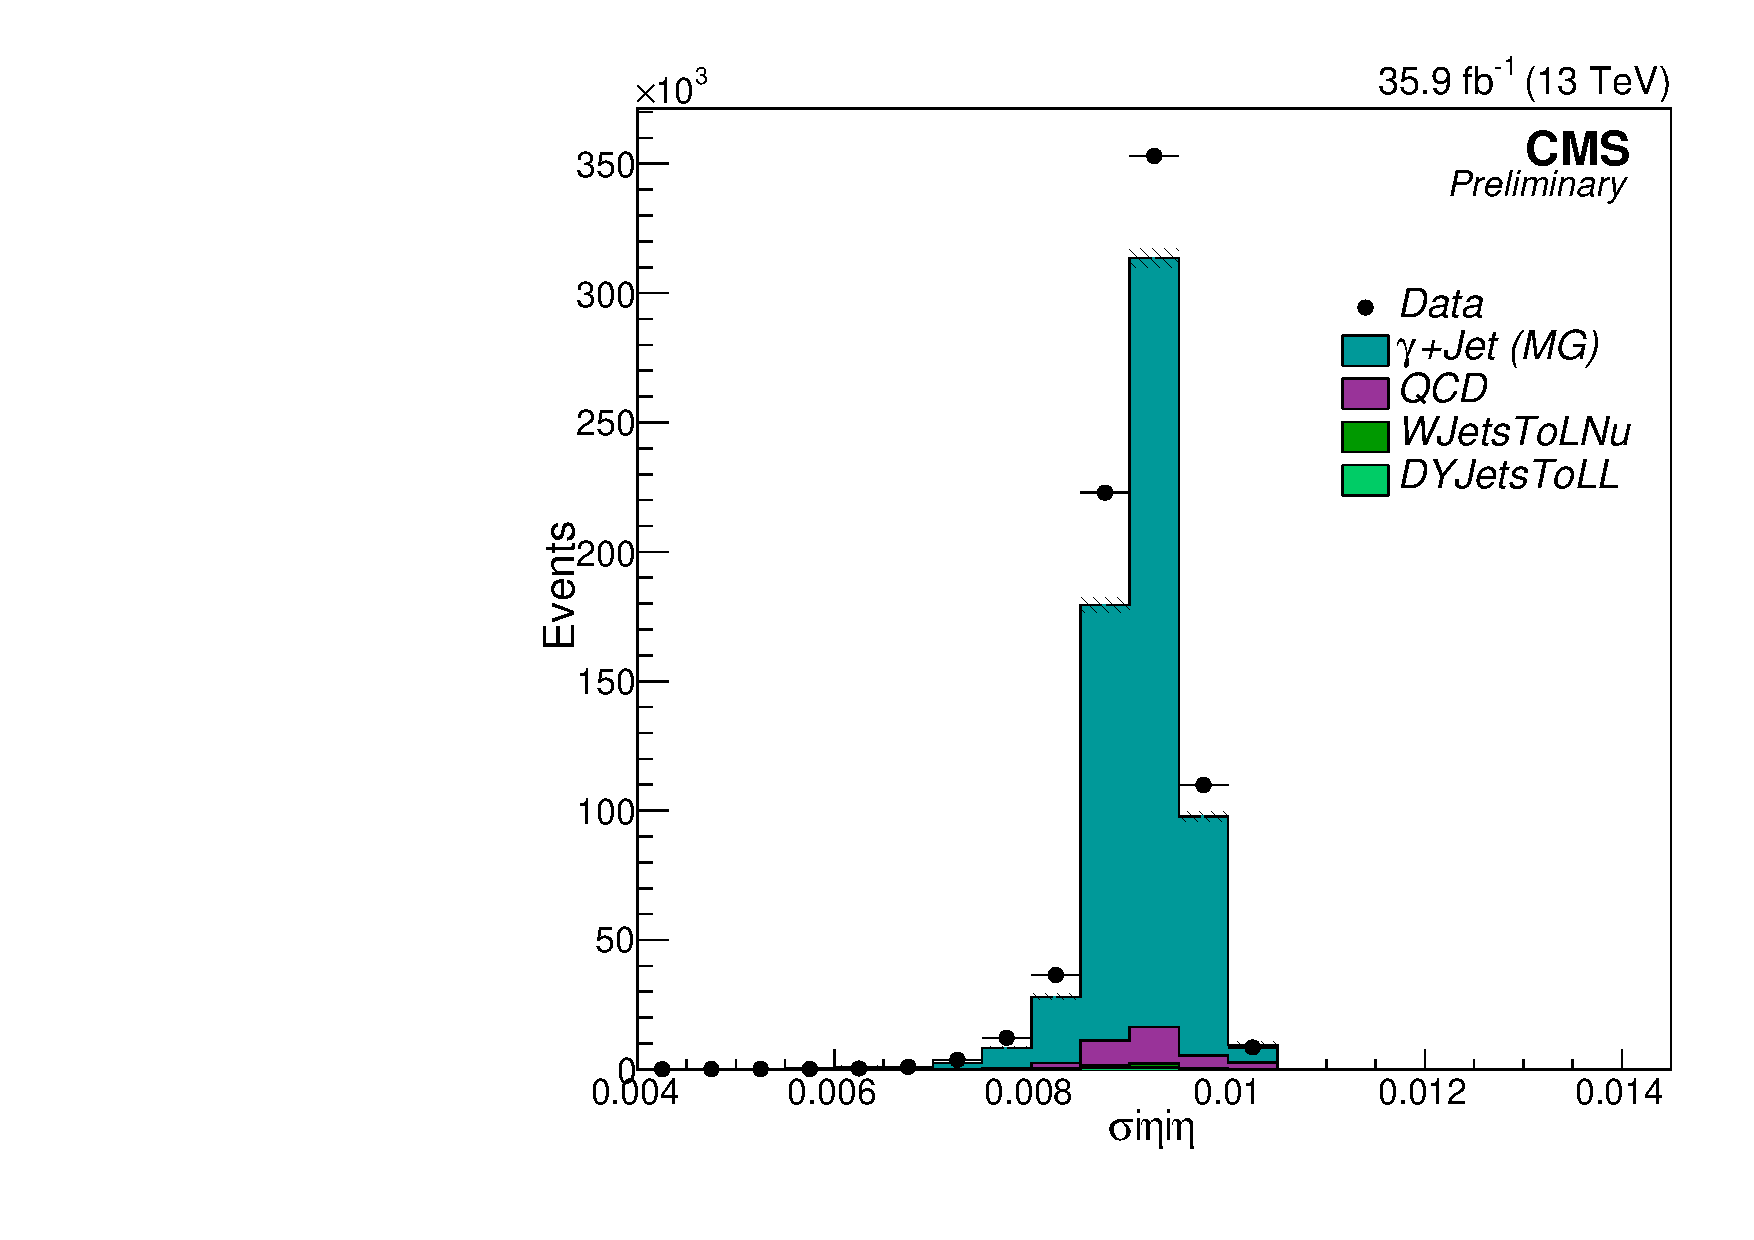
\includegraphics[width=7cm]{Chapter4/PhotonID/Ph_sigIetaIeta.pdf}} \hspace{0.2in}
 \subfloat[Single Tower H$/$E]{\label{fig:Ph_HoE}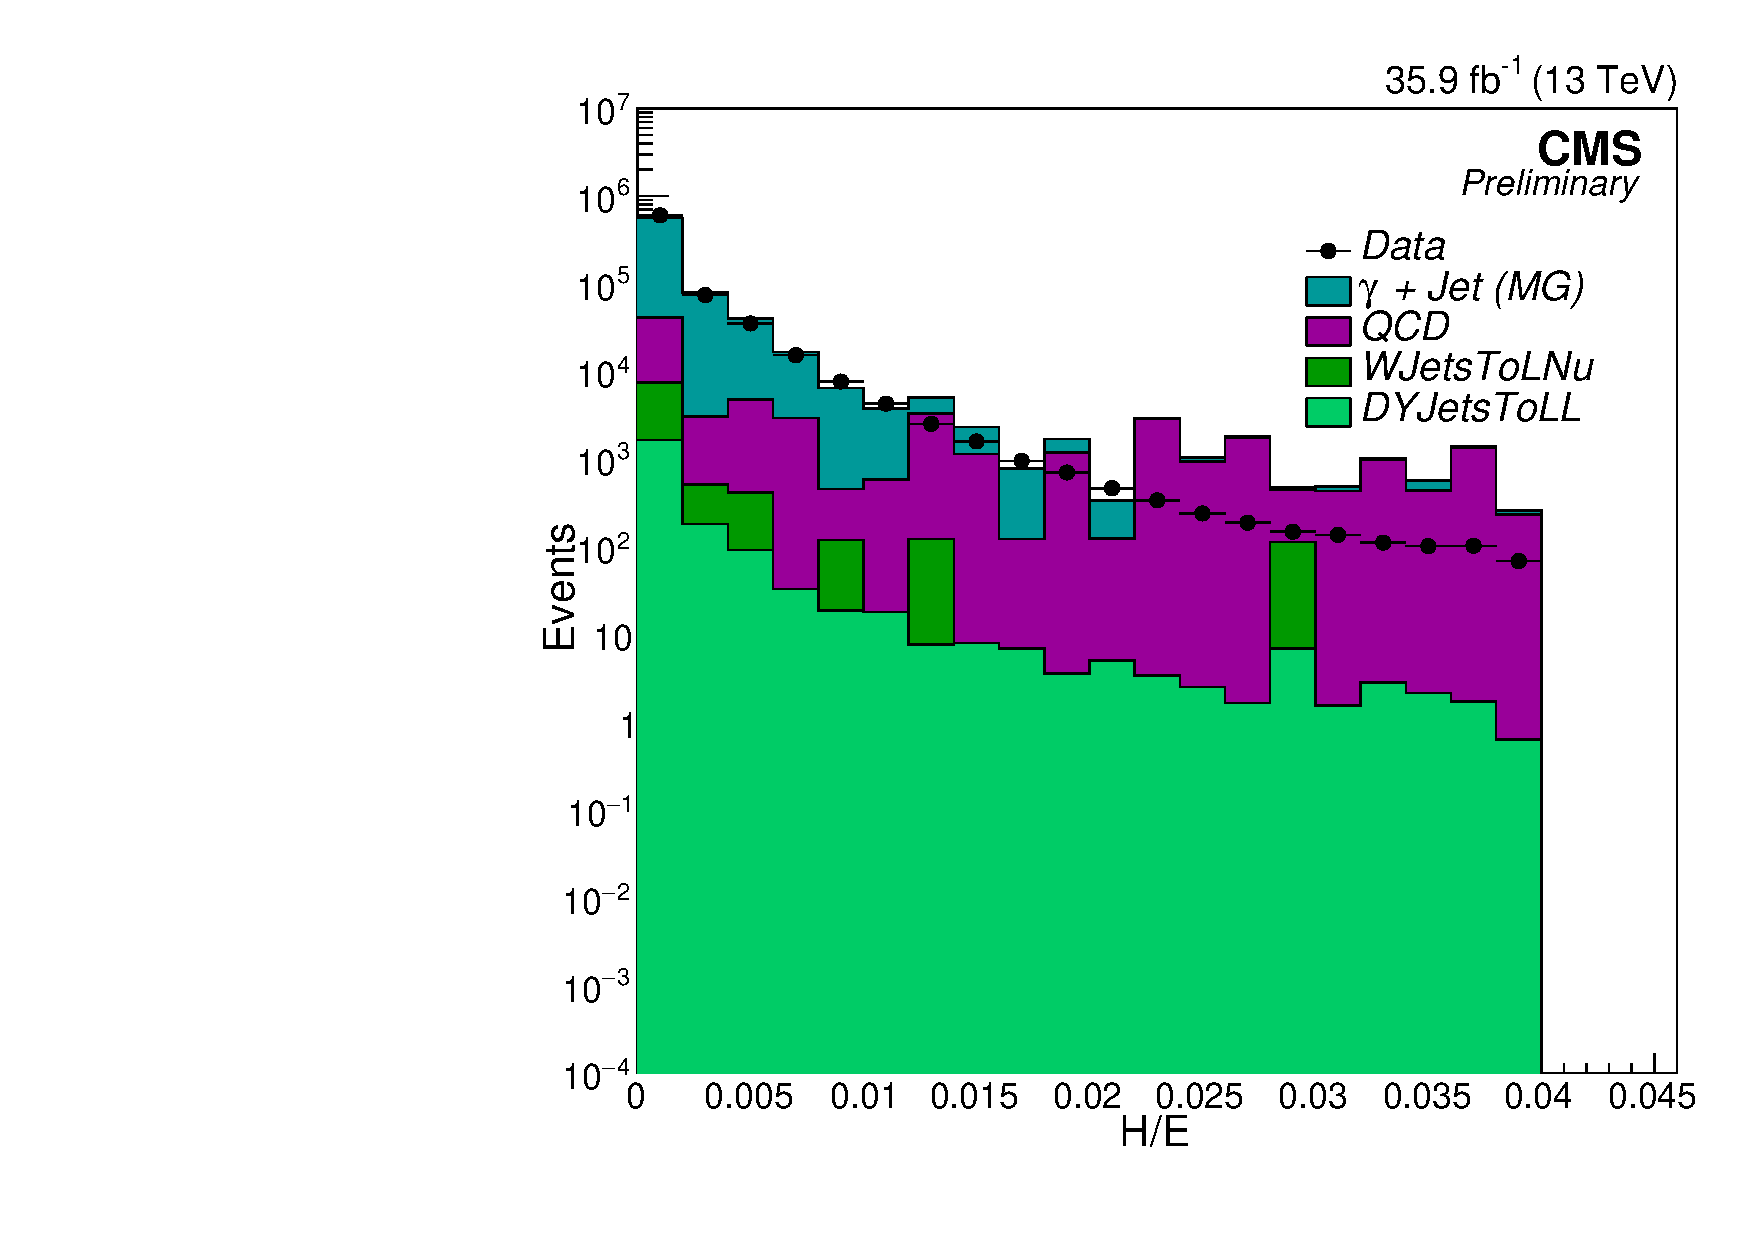
\includegraphics[width=7cm]{Chapter4/PhotonID/Ph_HoE.pdf}}\\
 \subfloat[R9]{\label{fig:Ph_r9}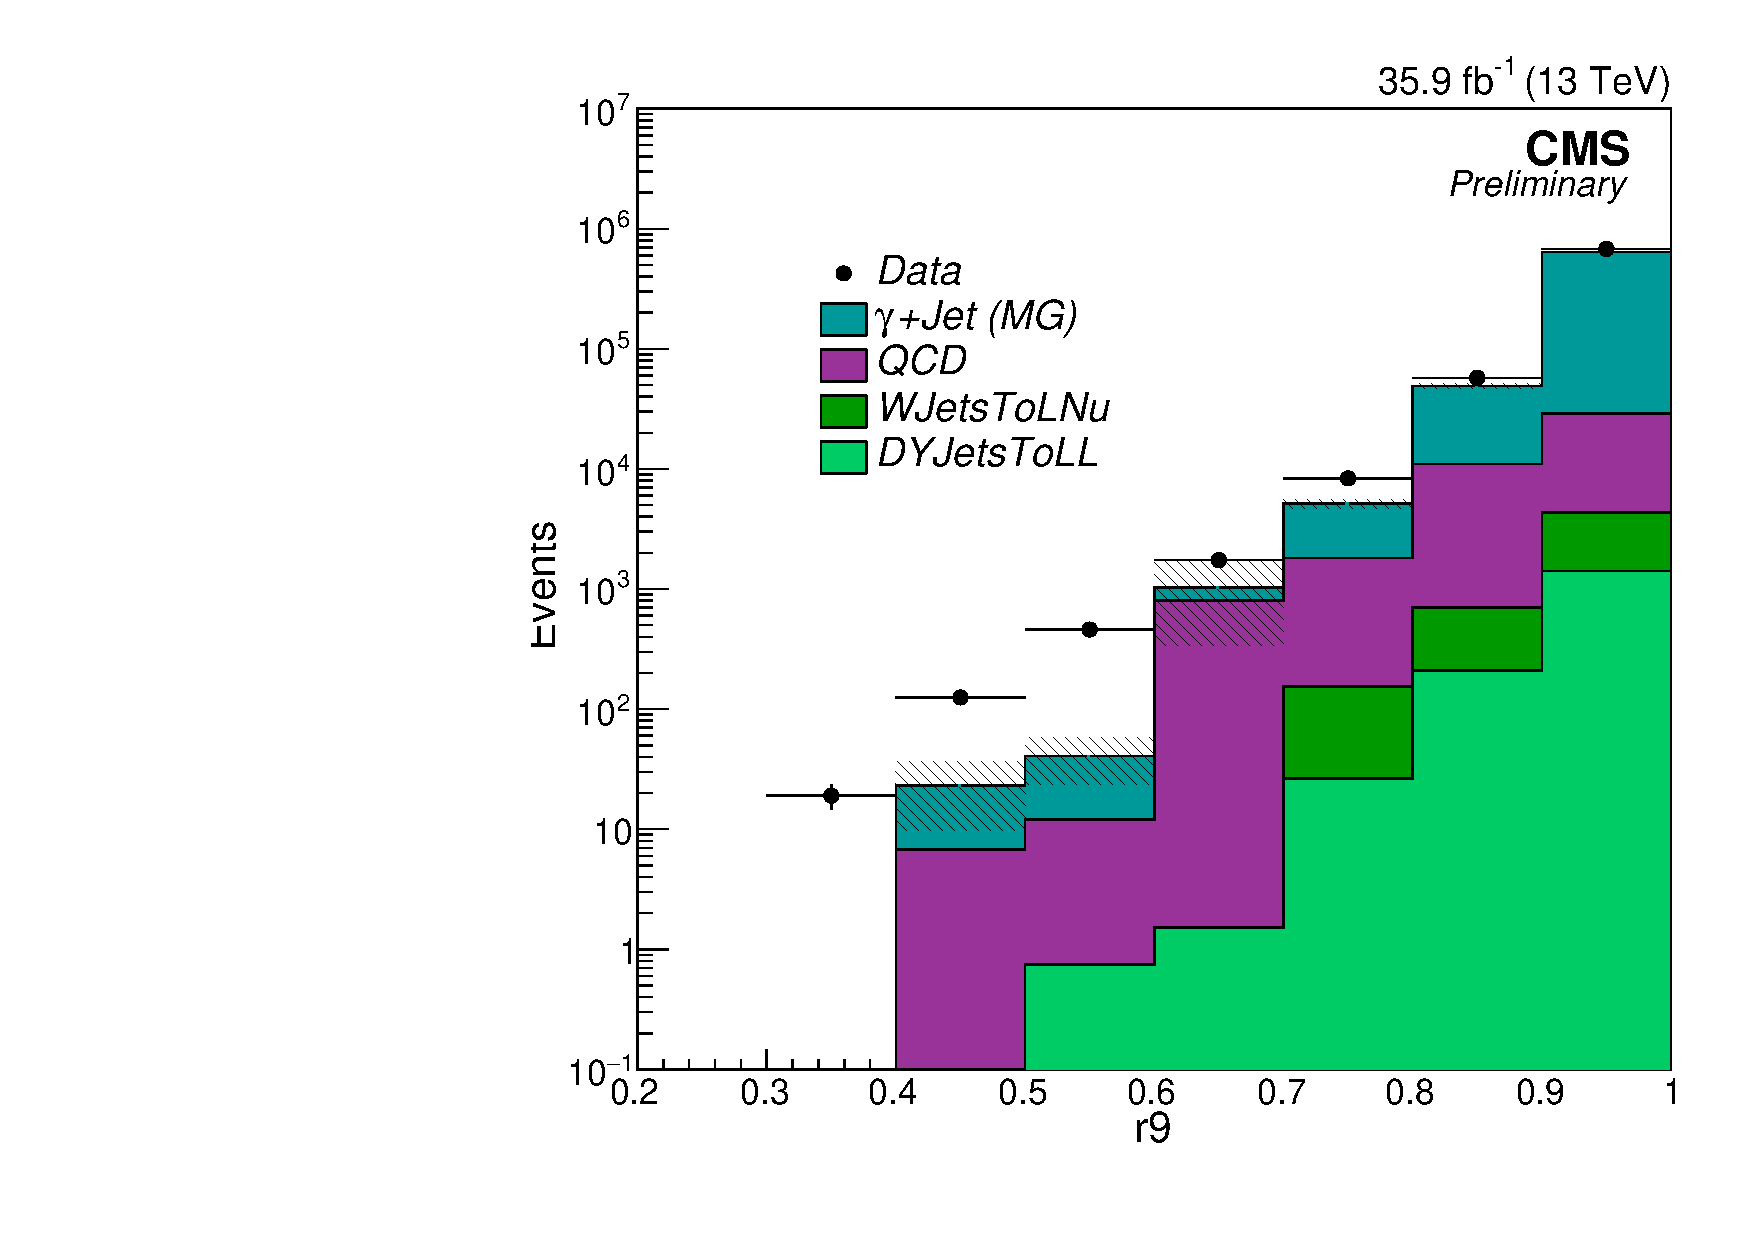
\includegraphics[width=7cm]{Chapter4/PhotonID/Ph_r9.pdf}}\hspace{0.2in}
 \subfloat[PF Charged Hadron Isolation]{\label{fig:Ph_Chiso}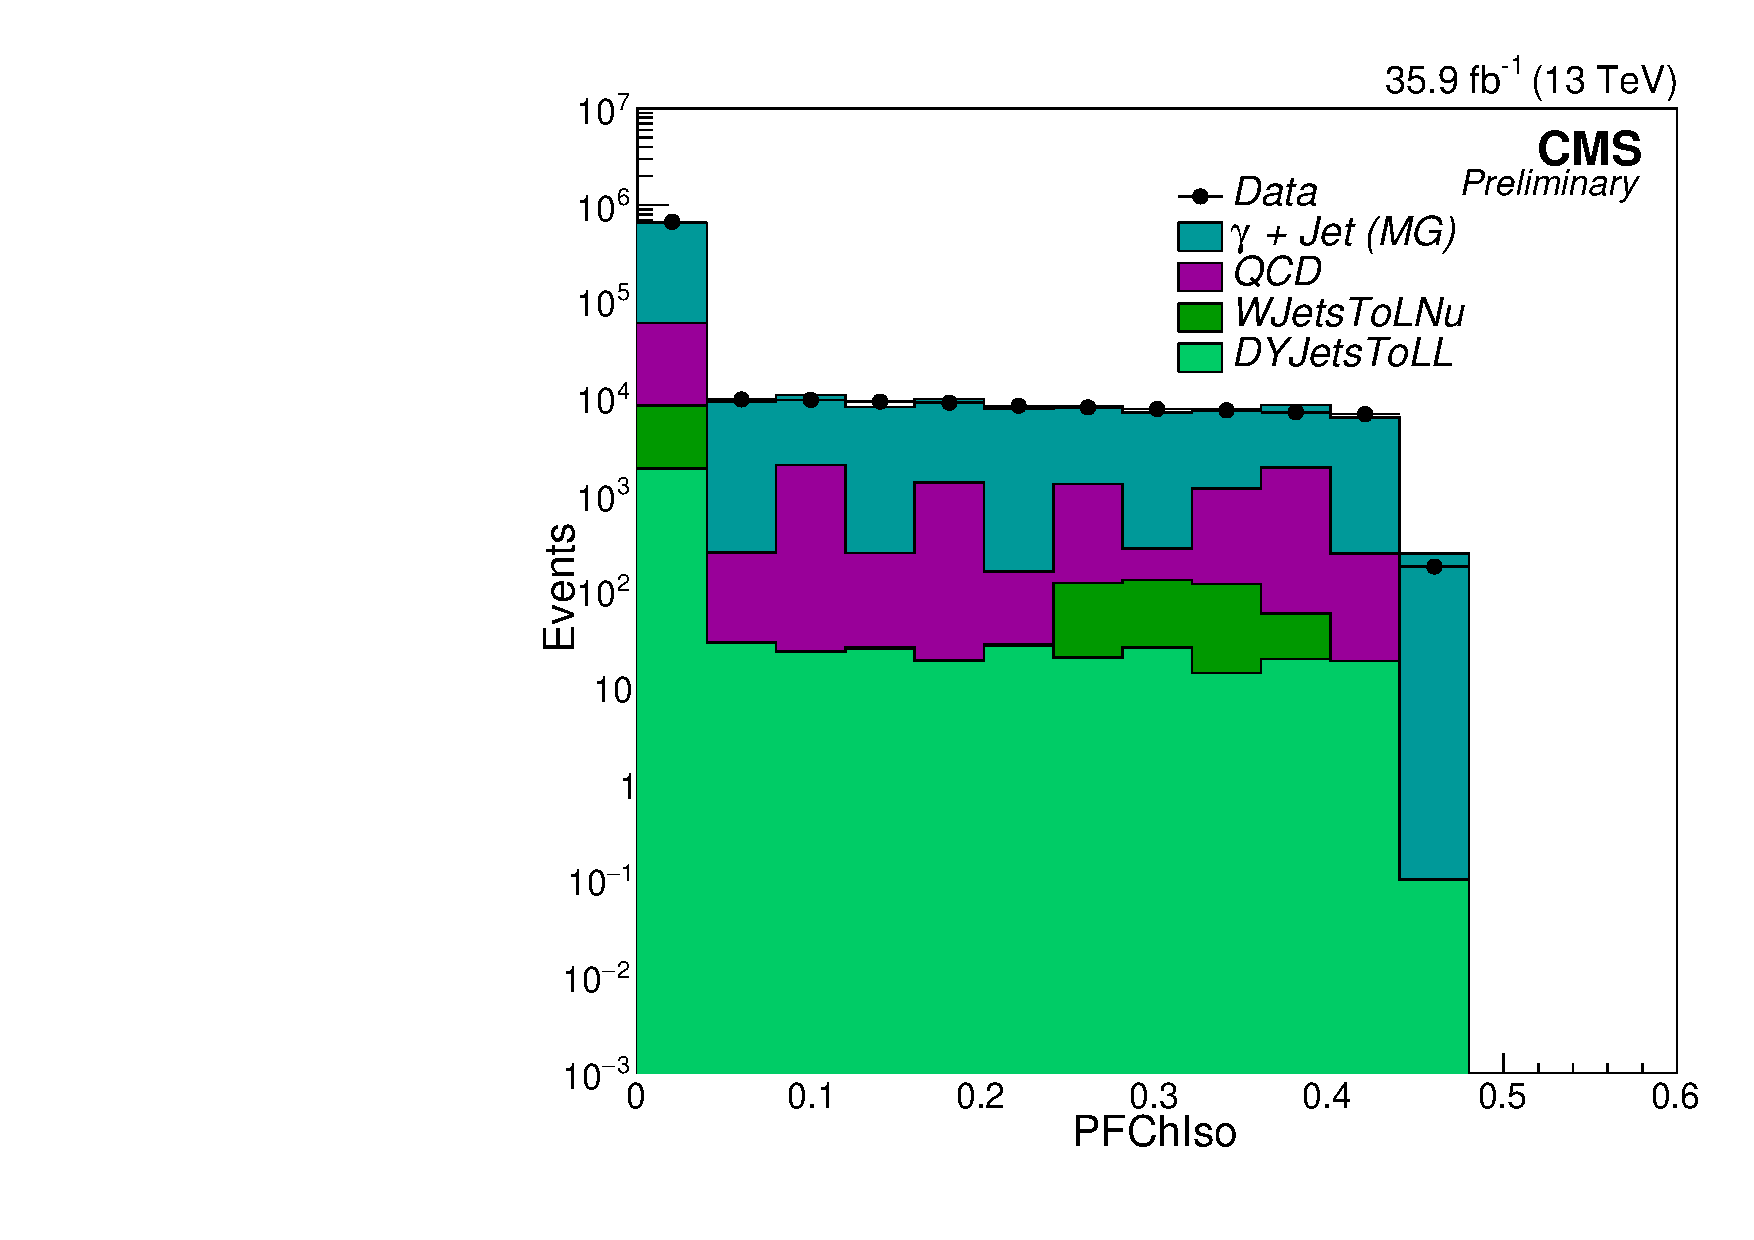
\includegraphics[width=7cm]{Chapter4/PhotonID/Ph_ChIso.pdf}} \\
 \subfloat[PF Photon Isolation]{\label{fig:Ph_Phiso}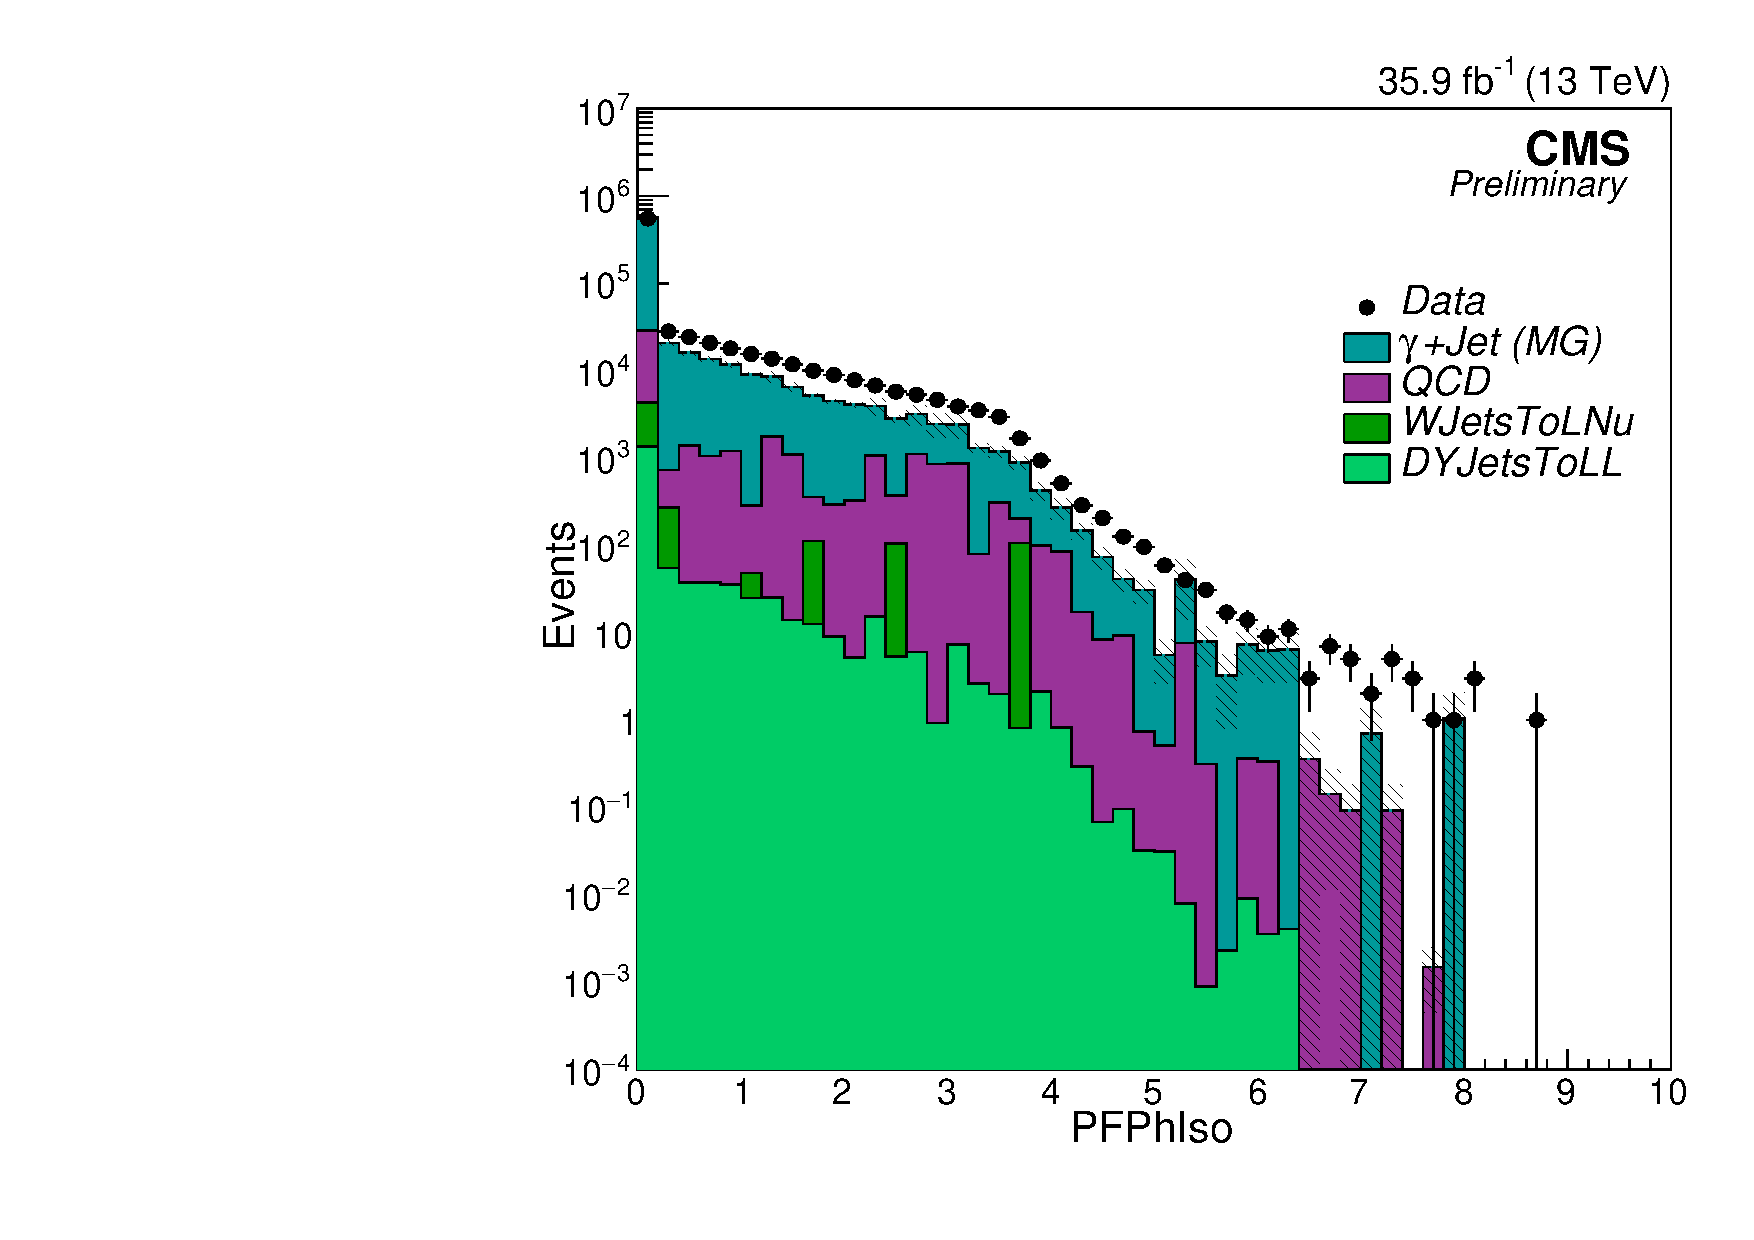
\includegraphics[width=7cm]{Chapter4/PhotonID/Ph_PhIso.pdf}} \hspace{0.2in}
 \subfloat[PF Neutral Hadron Isolation]{\label{fig:Ph_Neuiso}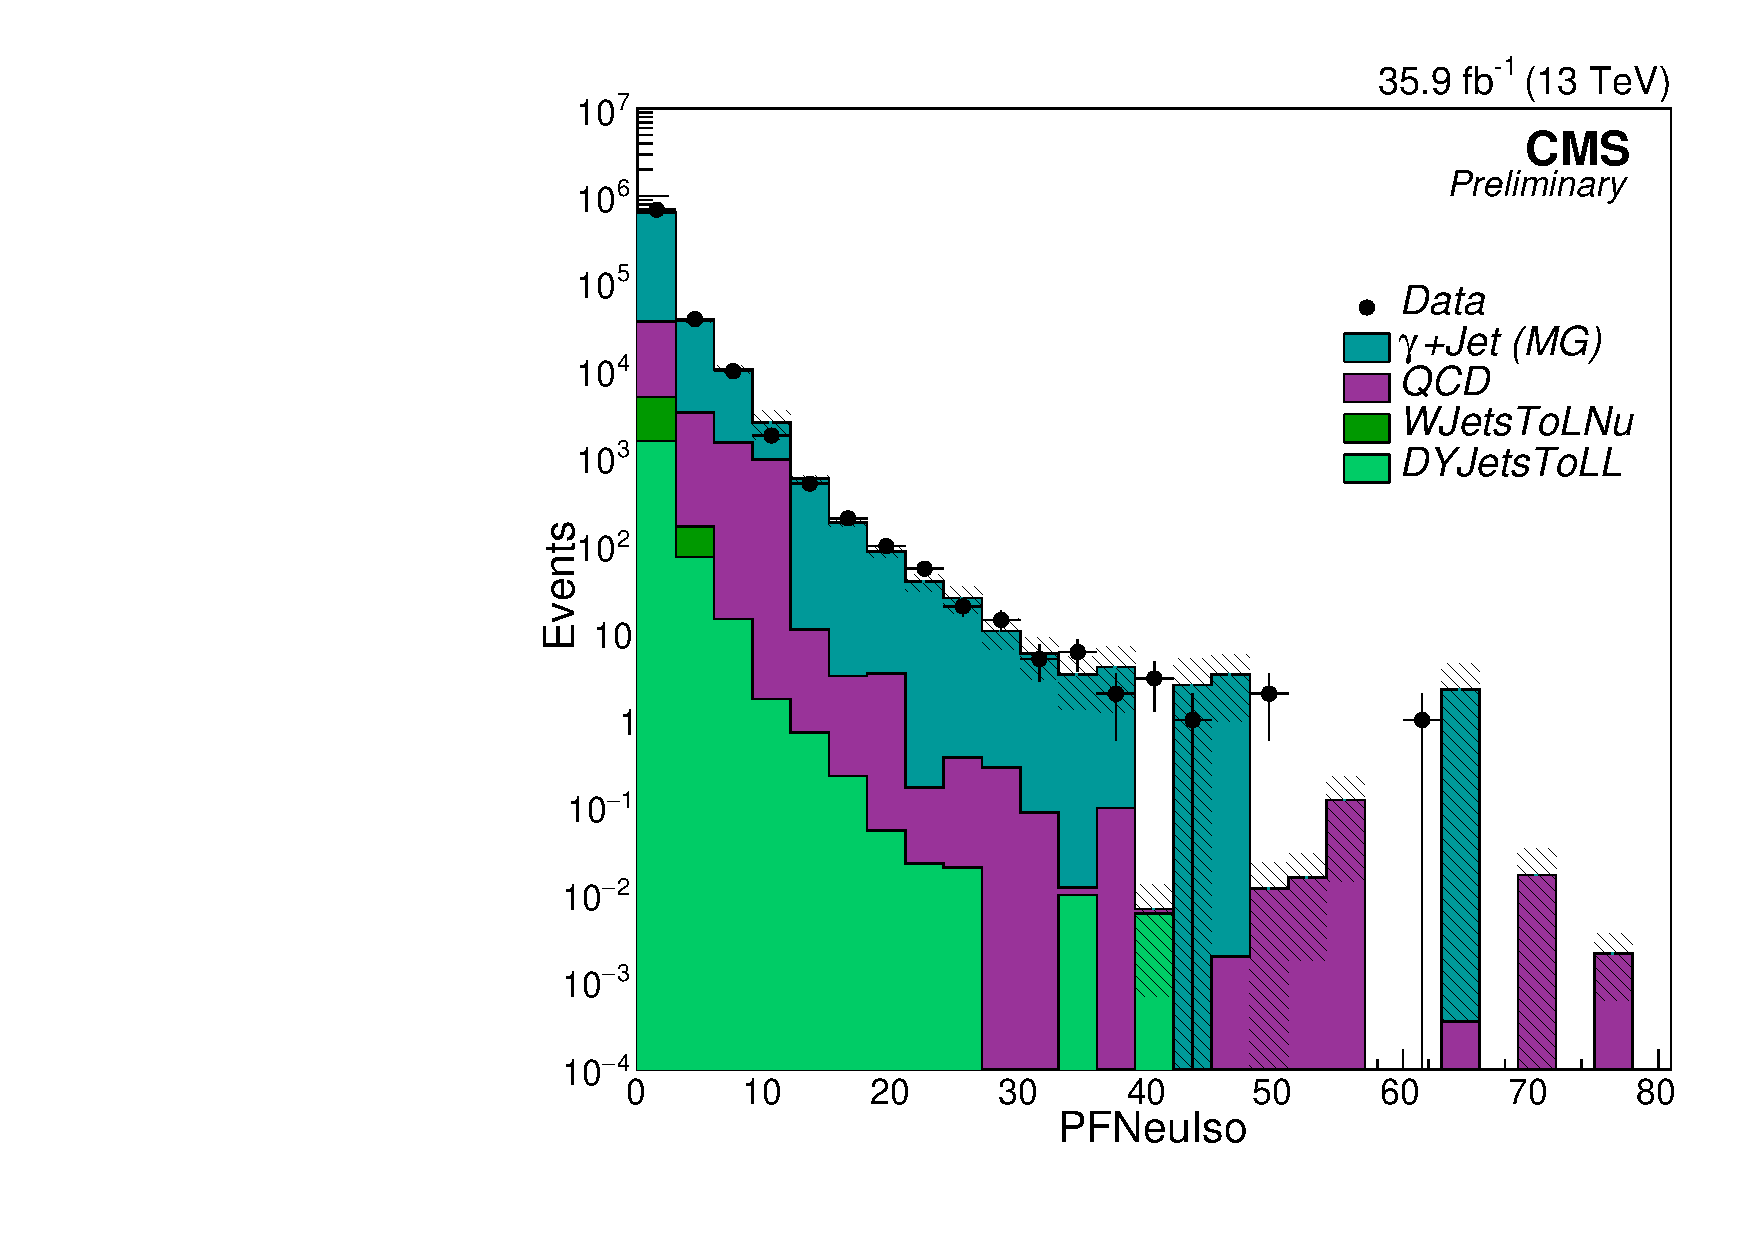
\includegraphics[width=7cm]{Chapter4/PhotonID/Ph_NeuIso.pdf}} 
\caption{Data-MC comparison of photon identification and isolation variables after final selection.}
\label{fig:PhIdnIso}
\end{figure}

\subsubsection{Overlap removal between $\gamjet$ and QCD dijet background}
The QCD sample used in this analysis has been generated using \pythia\ with the process: HardQCD::all $=$ ON, that is, at the generator level, all the processes like
gg $\rightarrow$ gg, gg $\rightarrow$ q$\bar{\textrm{q}}$, qg $\rightarrow$ qg, qq $\rightarrow$ qq, q$\bar{\textrm{q}}$ $\rightarrow$ gg,
q$\bar{\textrm{q}}$ $\rightarrow$ q$\bar{\textrm{q}}$ are allowed and are associated with initial and final state parton showers. Since quarks tend to hadronize
as soon as they are produced, the particles in parton showers appear to come from the primary vertex. Thus, the photons present in these parton showers
form the source of prompt photons in the QCD sample and can mimic a $\gamjet$ event.

However, in QCD, since the prompt photons come from the parton showers, they have a small $\Delta R$ separation from other gen particles. The same
is visible in \fig{\ref{fig:QCD_dr}} which shows the $\Delta R$ distribution between genPhotons and genPartons in the QCD sample. On the other hand, in $\gamjet$ sample,
the prompt photons come from the hard process and hence are largely separated from other particles as can be seen in \fig{\ref{fig:GJet_dr}}.

The events containing these prompt photons in QCD sample are removed in order to avoid double counting of events between $\gamjet$ and QCD dijet samples.
The procedure followed to remove the overlap is summarized as follows:

\begin{itemize}[leftmargin=*]
\item In a QCD event, a gen photon corresponding to the selected reco photon is searched by requiring, gen particle ID $=$ 22,
  $\Delta$R(Gen, Reco) $<$ 0.1 and $\frac{{\Delta}\pt}{\pt}$(Gen, Reco) $<$ 0.1. Once the gen photon is found, its prompt status is checked
  using its gen level properties. If it is prompt, the event is removed from the event collection, otherwise not.
\item Since $\gamjet$ MC sample has a gen level cut of $\Delta$R($\gamma$, Parton) $>$ 0.05, so the events with only $\Delta$R($\gamma$, Parton) $>$ 0.05
  are removed from the QCD sample.
\item The events with $\Delta$R($\gamma$, Parton) $<$ 0.05 (if any) are, then, removed from the $\gamjet$ MC sample.
\end{itemize}

The \fig{\ref{fig:stitch_dr}} shows the stitching of the two samples in $\Delta$R after overlap removal. It can be seen that the stitching behaves nicely at the
$\Delta$R cut.

\begin{figure}[htbp]
\centering
\subfloat[QCD]{\label{fig:QCD_dr}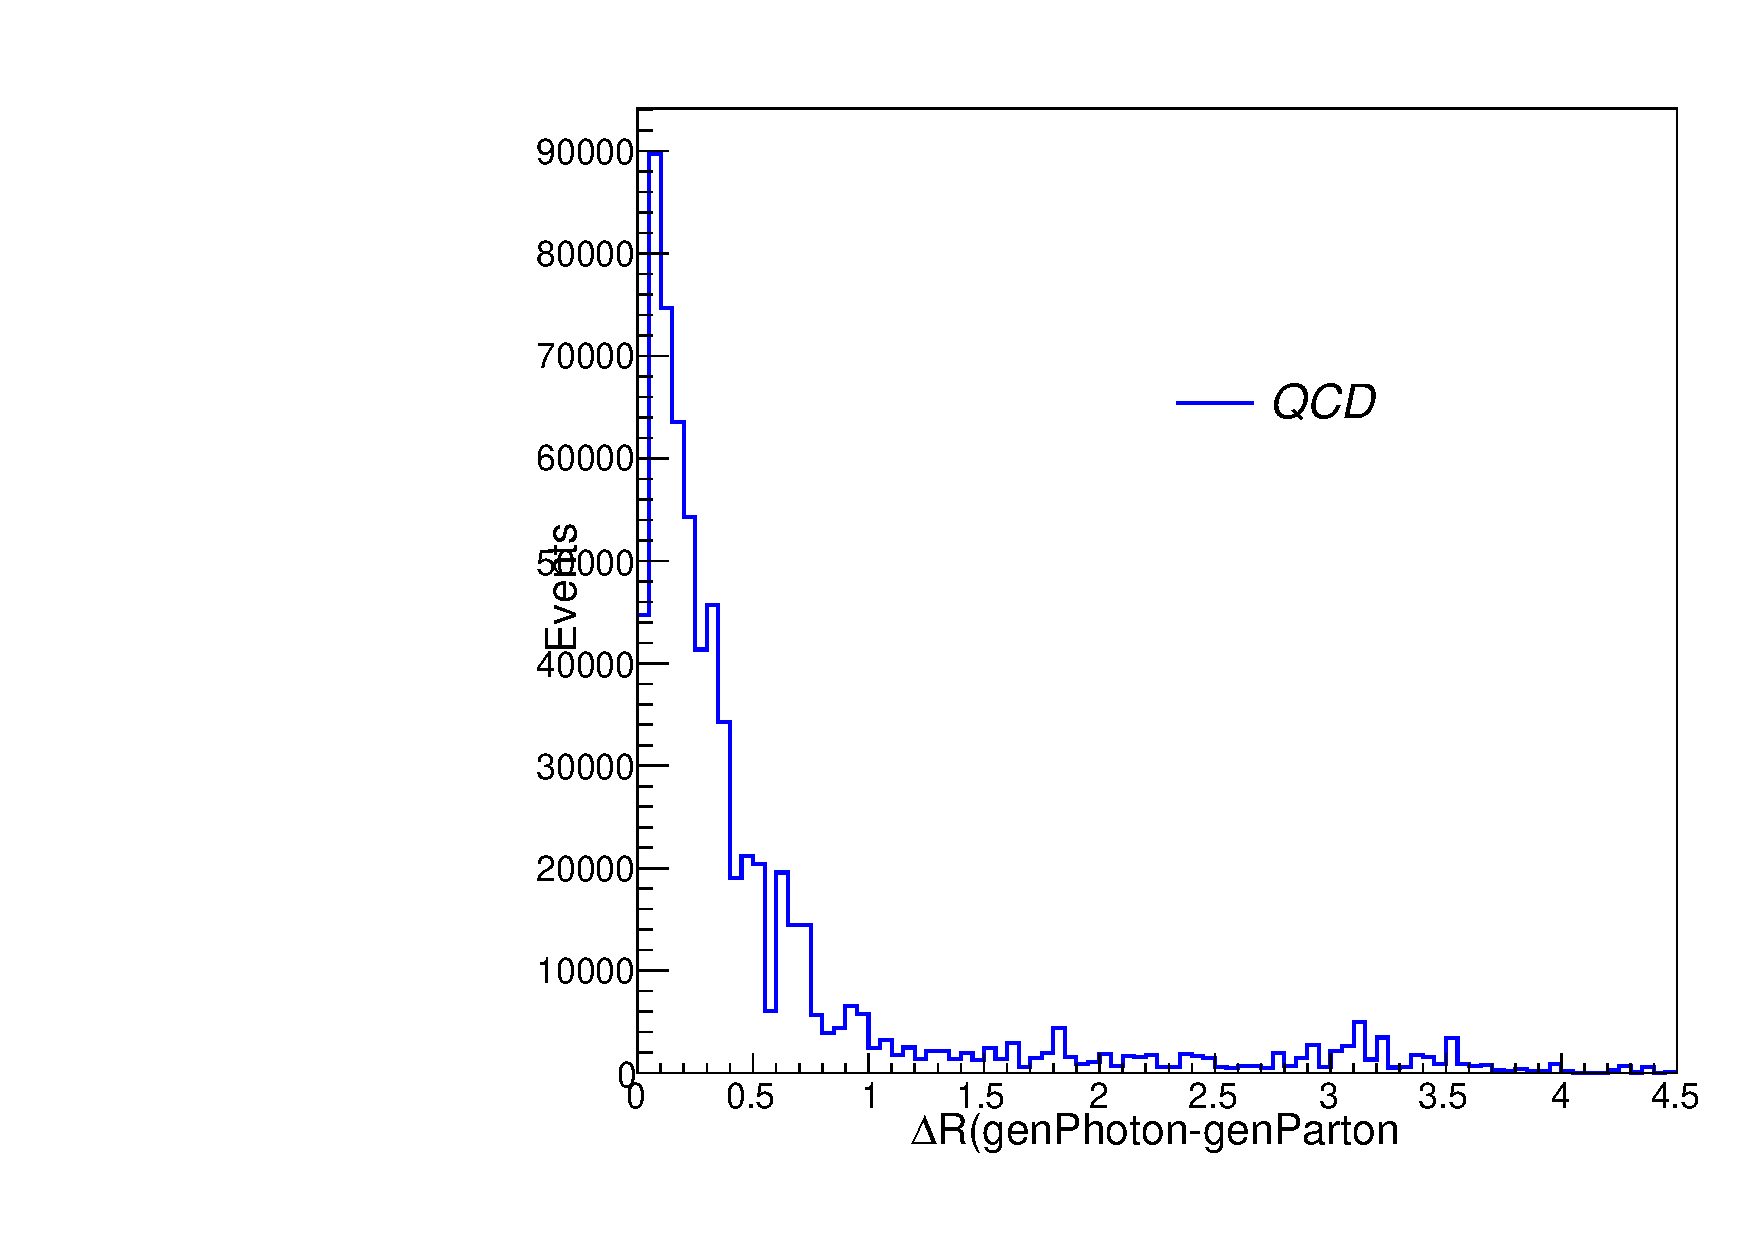
\includegraphics[width=5.3cm]{Chapter4/QCD_OvrlpRemoval/QCD_genRecoDR_without_PhIsolation.pdf}}
\subfloat[$\gamjet$]{\label{fig:GJet_dr}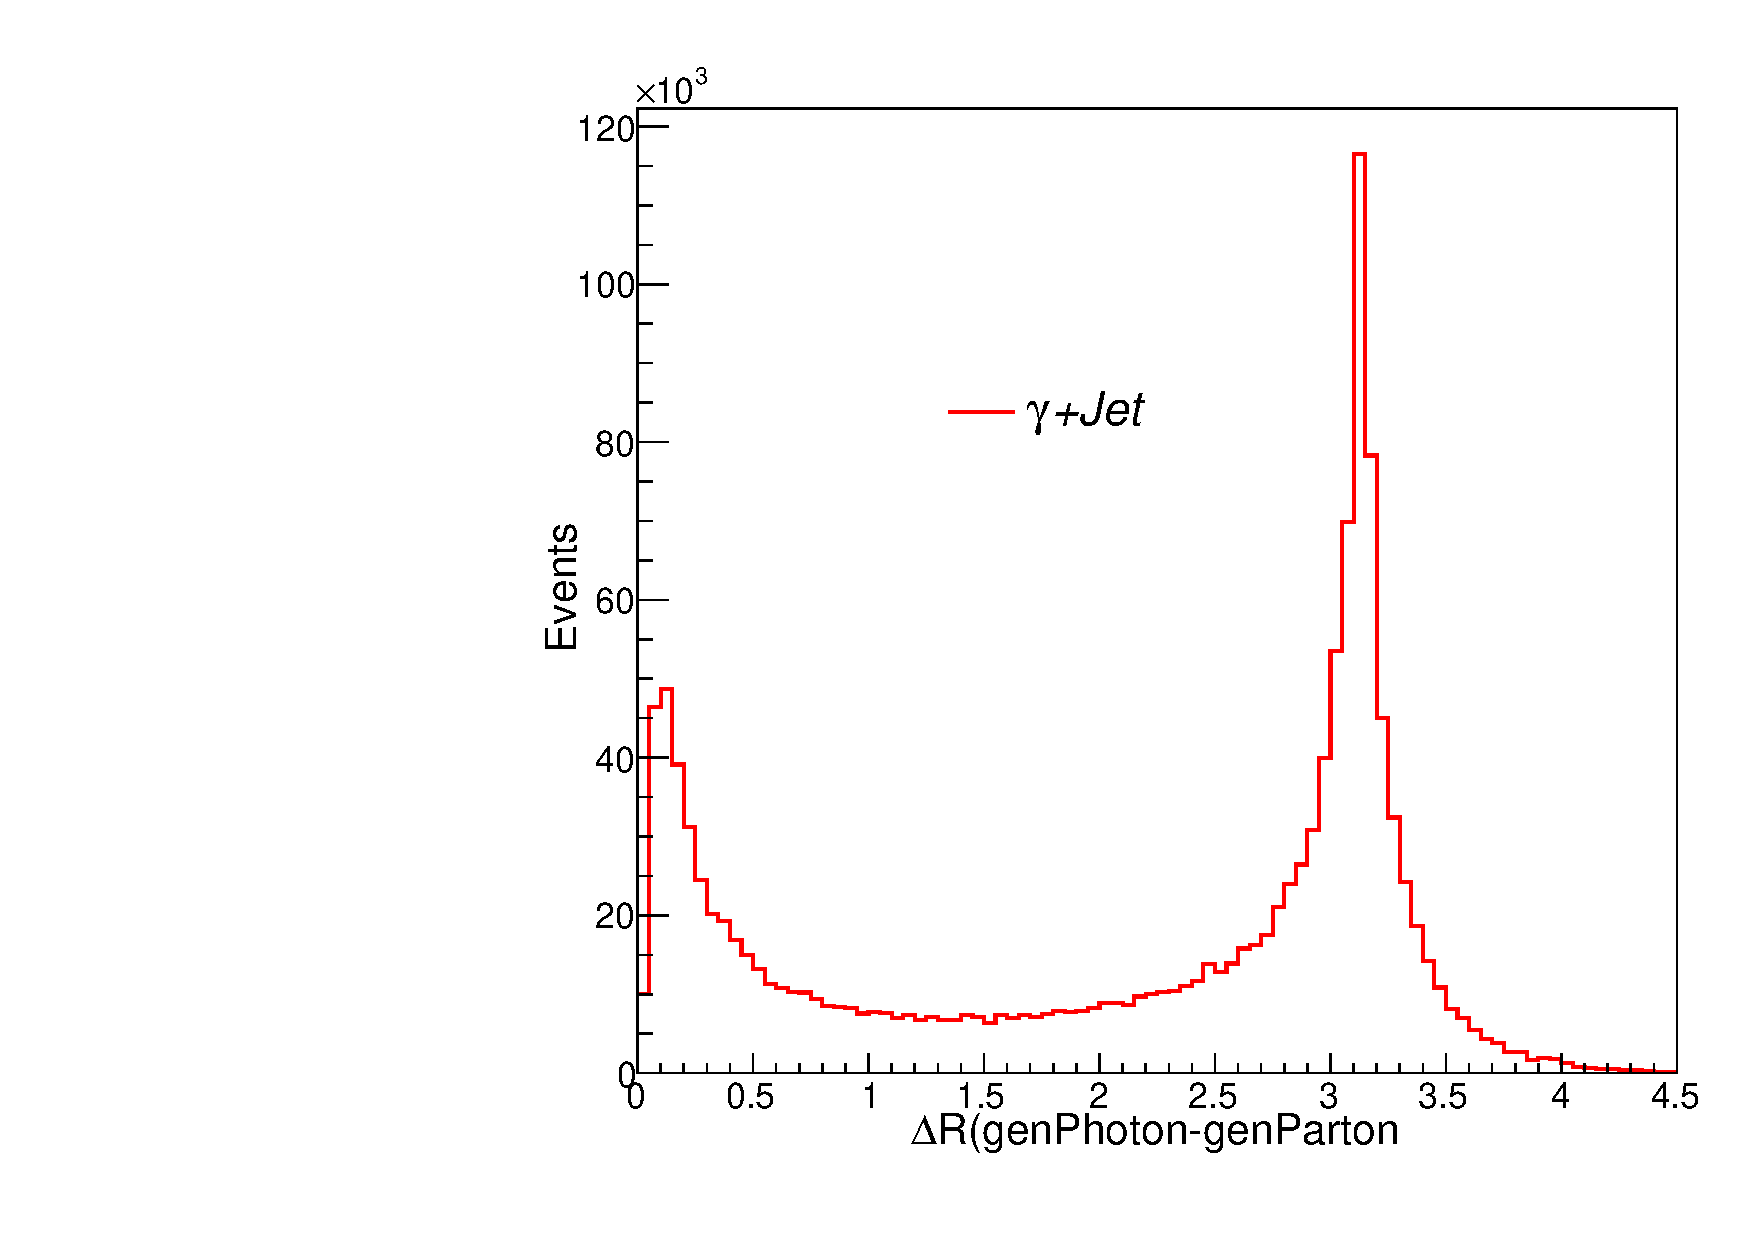
\includegraphics[width=5.3cm]{Chapter4/QCD_OvrlpRemoval/GJ_genRecoDR_without_PhIsolation.pdf}} 
\subfloat[Stitching of QCD and $\gamjet$]{\label{fig:stitch_dr}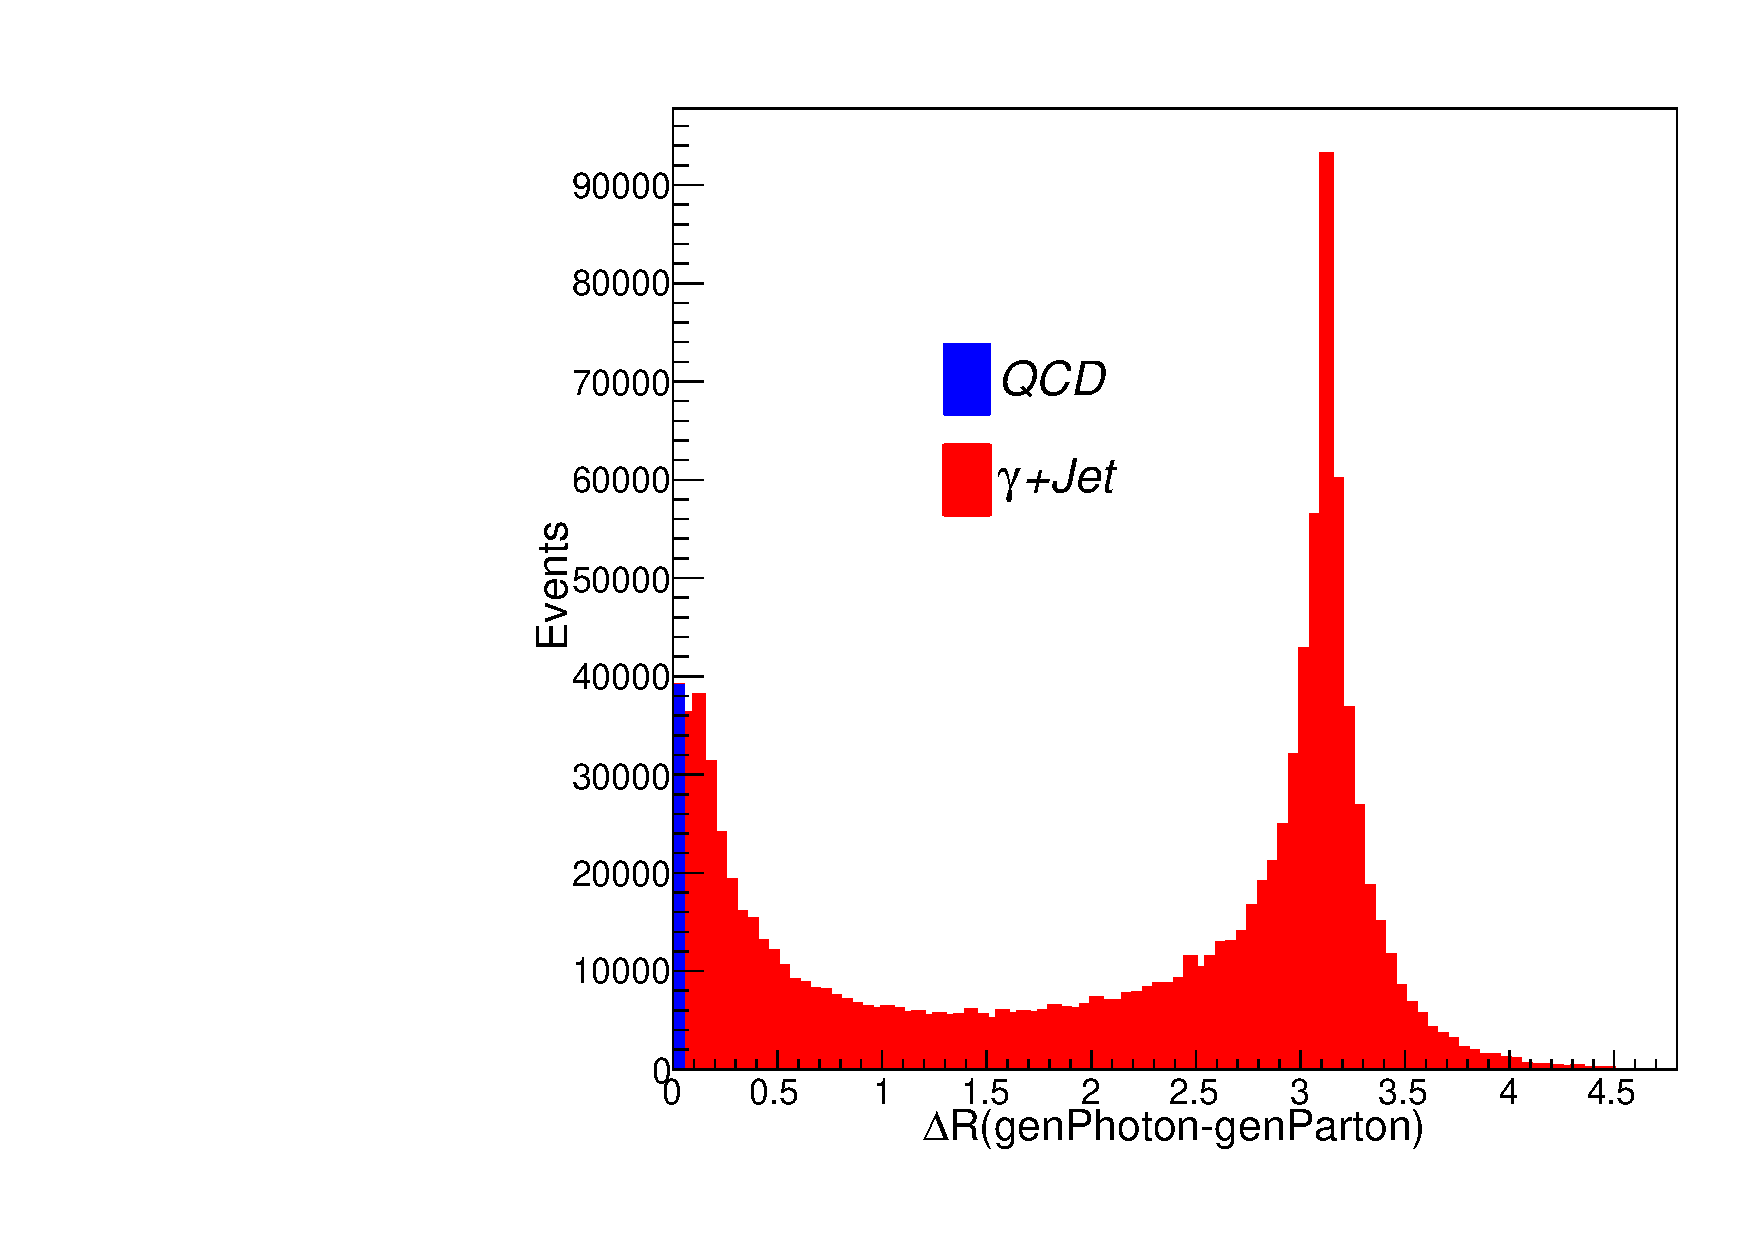
\includegraphics[width=5.3cm]{Chapter4/QCD_OvrlpRemoval/Stacked_QCD-GJ_genRecoDR0p05_BeforePhIsolation_AfterOverlapRemovalInQCDnGjet.pdf}}
\caption{$\Delta R$ distribution between prompt gen photon matched to selected reco photon and other gen particles: (a) QCD before overlap removal, (b) $\gamjet$ before overlap removal, (c) Stitching of QCD and $\gamjet$ after overlap removal.}
\label{fig:genDR}
\end{figure}

\subsection{Analysis object selection: Jet}
Events containing a good photon candidate are further inspected for the presence of an AK4 jet using the identification criteria mentioned in \sectn{\ref{Se:JetID}}.
The cut-off values used for different variables is listed below. The jets qualifying this selection are required to be away from the selected photon
by $\Delta$R $>$ 0.5, to ensure that they are different objects and not the fragments of the same particle.
\vspace{-0.1in}
\begin{itemize}[leftmargin=*]
\item Charged hadron fraction $>$ 0.
\item Neutral hadron fraction $<$ 0.90.
\item Charged EM fraction $<$ 0.99.
\item Neutral EM fraction $<$ 0.90.
\item Number of constituents $>$ 1.
\item Charged multiplicity $>$ 0.
\end{itemize}

Out of the selected jet collection, the jet with highest \pt is considered and is required to have a \pt $>$ 170\unit{GeV} and $|\eta|$ $<$ 2.4.
A nearly symmetric cut on the \pt of photon and jet is considered since the photons and jets in the signal samples are distributed symmetrically in \pt as can be seen for
\qstar samples in \fig{\ref{fig:qstar_ptcomp}}. 

In order to overcome the non-linear response of the detector, L1, L2, L3 and L2L3 corrections as mentioned in \sectn{\ref{Se:JetEnCorr}} are applied.
A comparison of Data and MC for different jet variables after final selection is shown in \fig{\ref{fig:JetId}}.

\begin{figure}[h]
\centering
 \subfloat[M$_{\qstar}$ = 2.0\unit{TeV}]{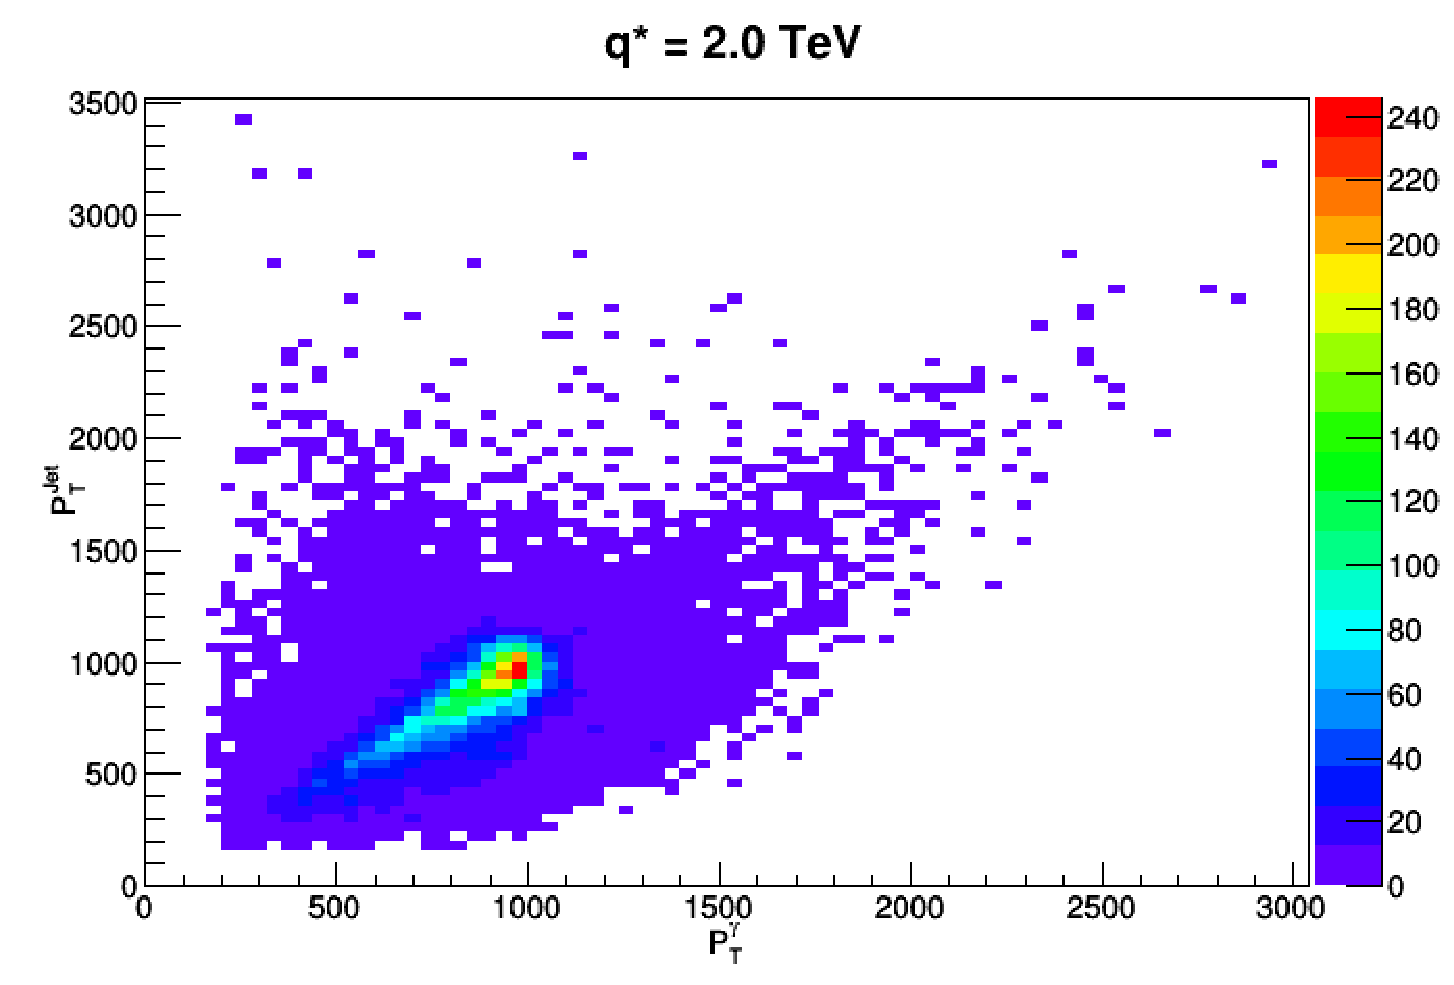
\includegraphics[width=7.0cm]{Chapter4/Signal_PTcomp/PtPh_vs_PtJet_qstar_2tev.pdf}} \hspace{0.2in}
 \subfloat[M$_{\qstar}$ = 4.0\unit{TeV}]{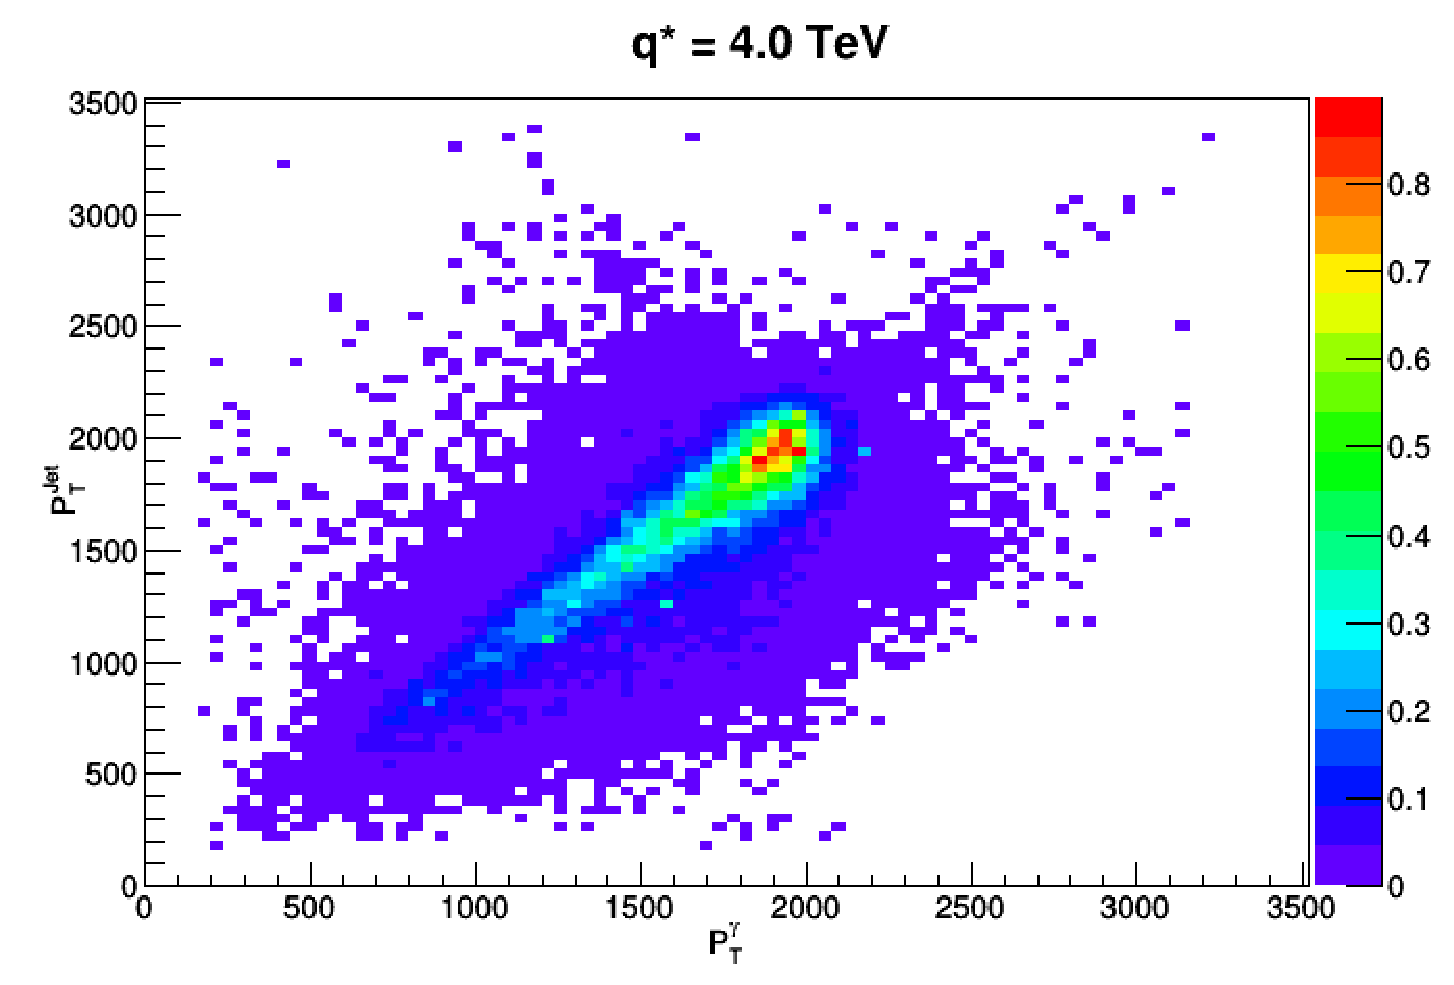
\includegraphics[width=7.0cm]{Chapter4/Signal_PTcomp/PtPh_vs_PtJet_qstar_4tev.pdf}}
\caption{$\pt^{\gamma}$ vs. $\pt^{\textrm{jet}}$ in 2-dimensional representation for \qstar signals.}
\label{fig:qstar_ptcomp}
\end{figure}

\begin{figure}[htpb]
\centering
\subfloat[Neutral Hadron Energy Fraction]{\label{fig:Jet_NHEF}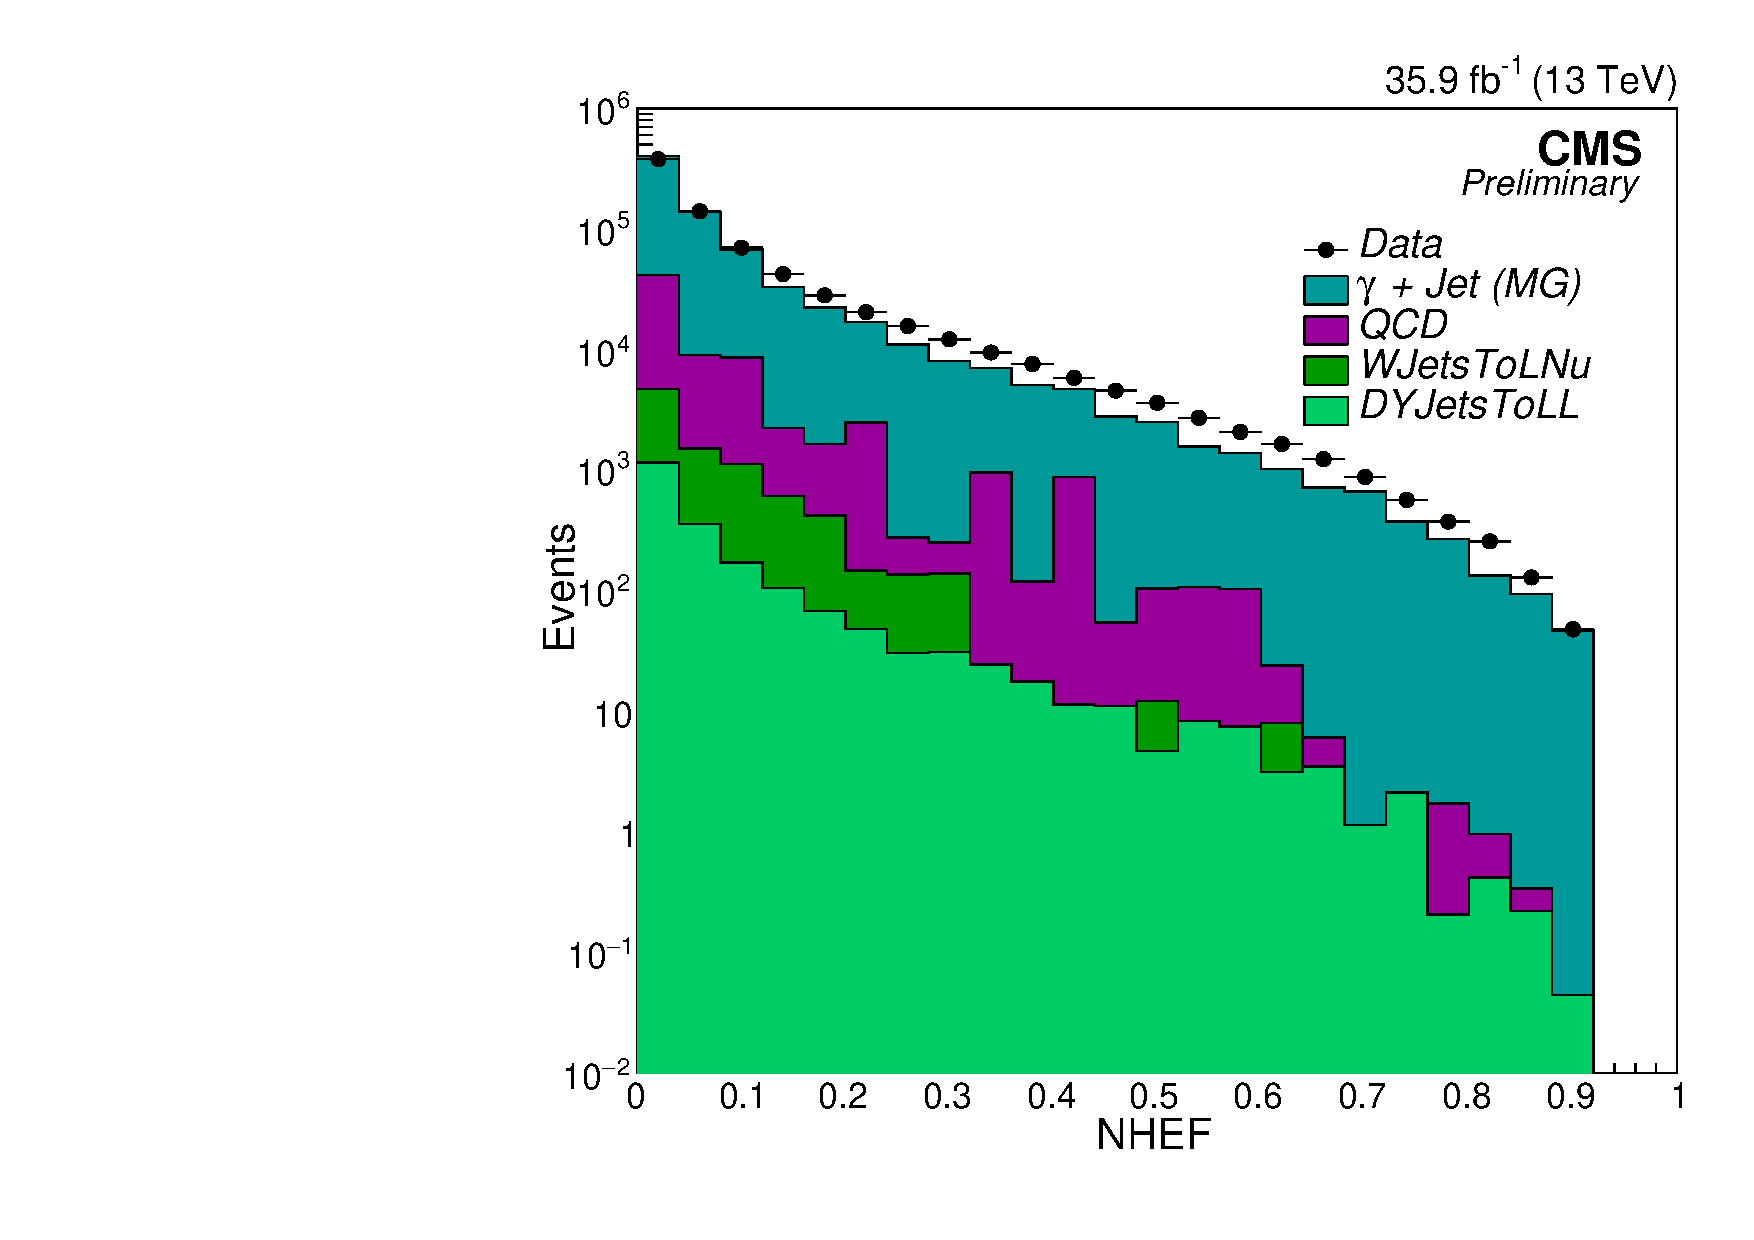
\includegraphics[width=7cm]{Chapter4/JetID/Jet_NHEF.pdf}} \hspace{0.2in}
\subfloat[Charged Hadron Energy Fraction]{\label{fig:Jet_CHEF}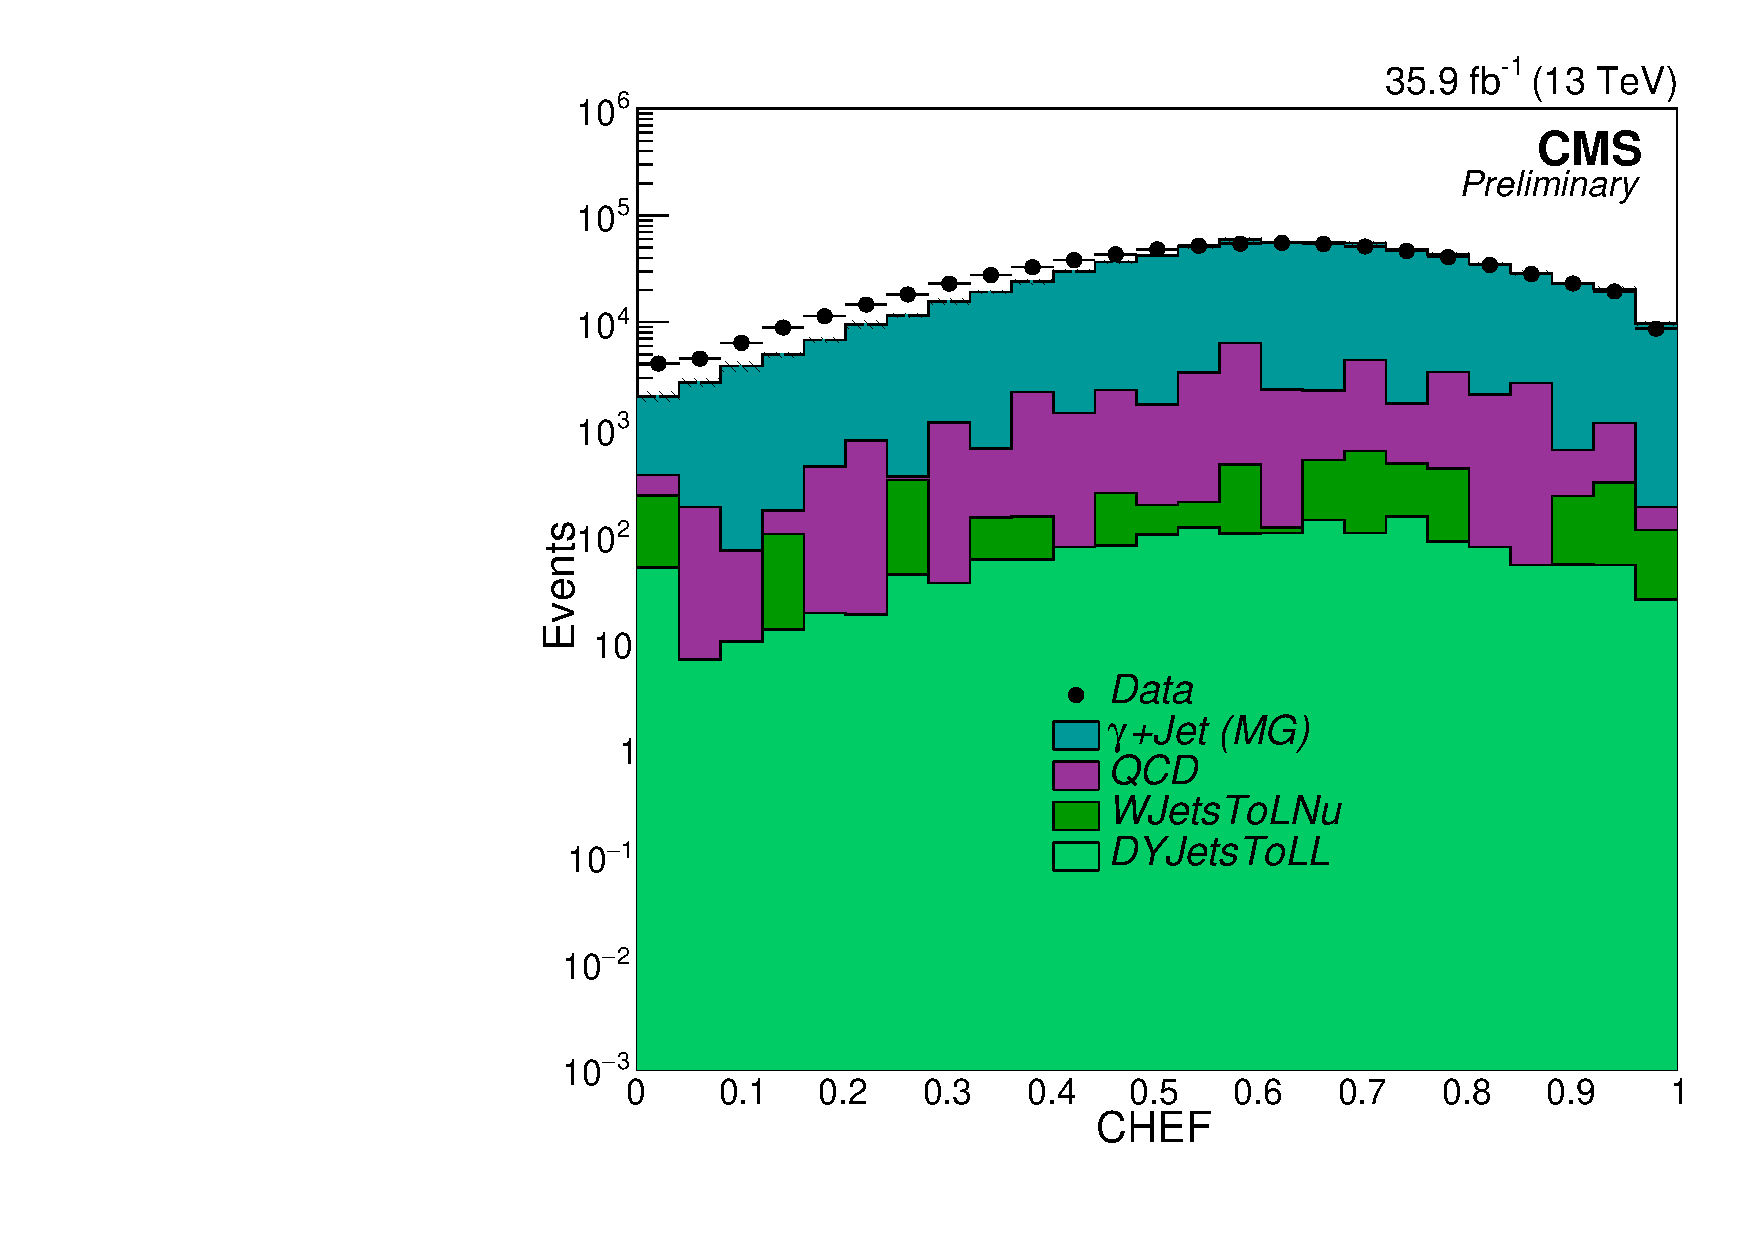
\includegraphics[width=7cm]{Chapter4/JetID/Jet_CHEF.pdf}} \\
\subfloat[Neutral EM Energy Fraction]{\label{fig:Jet_NEEF}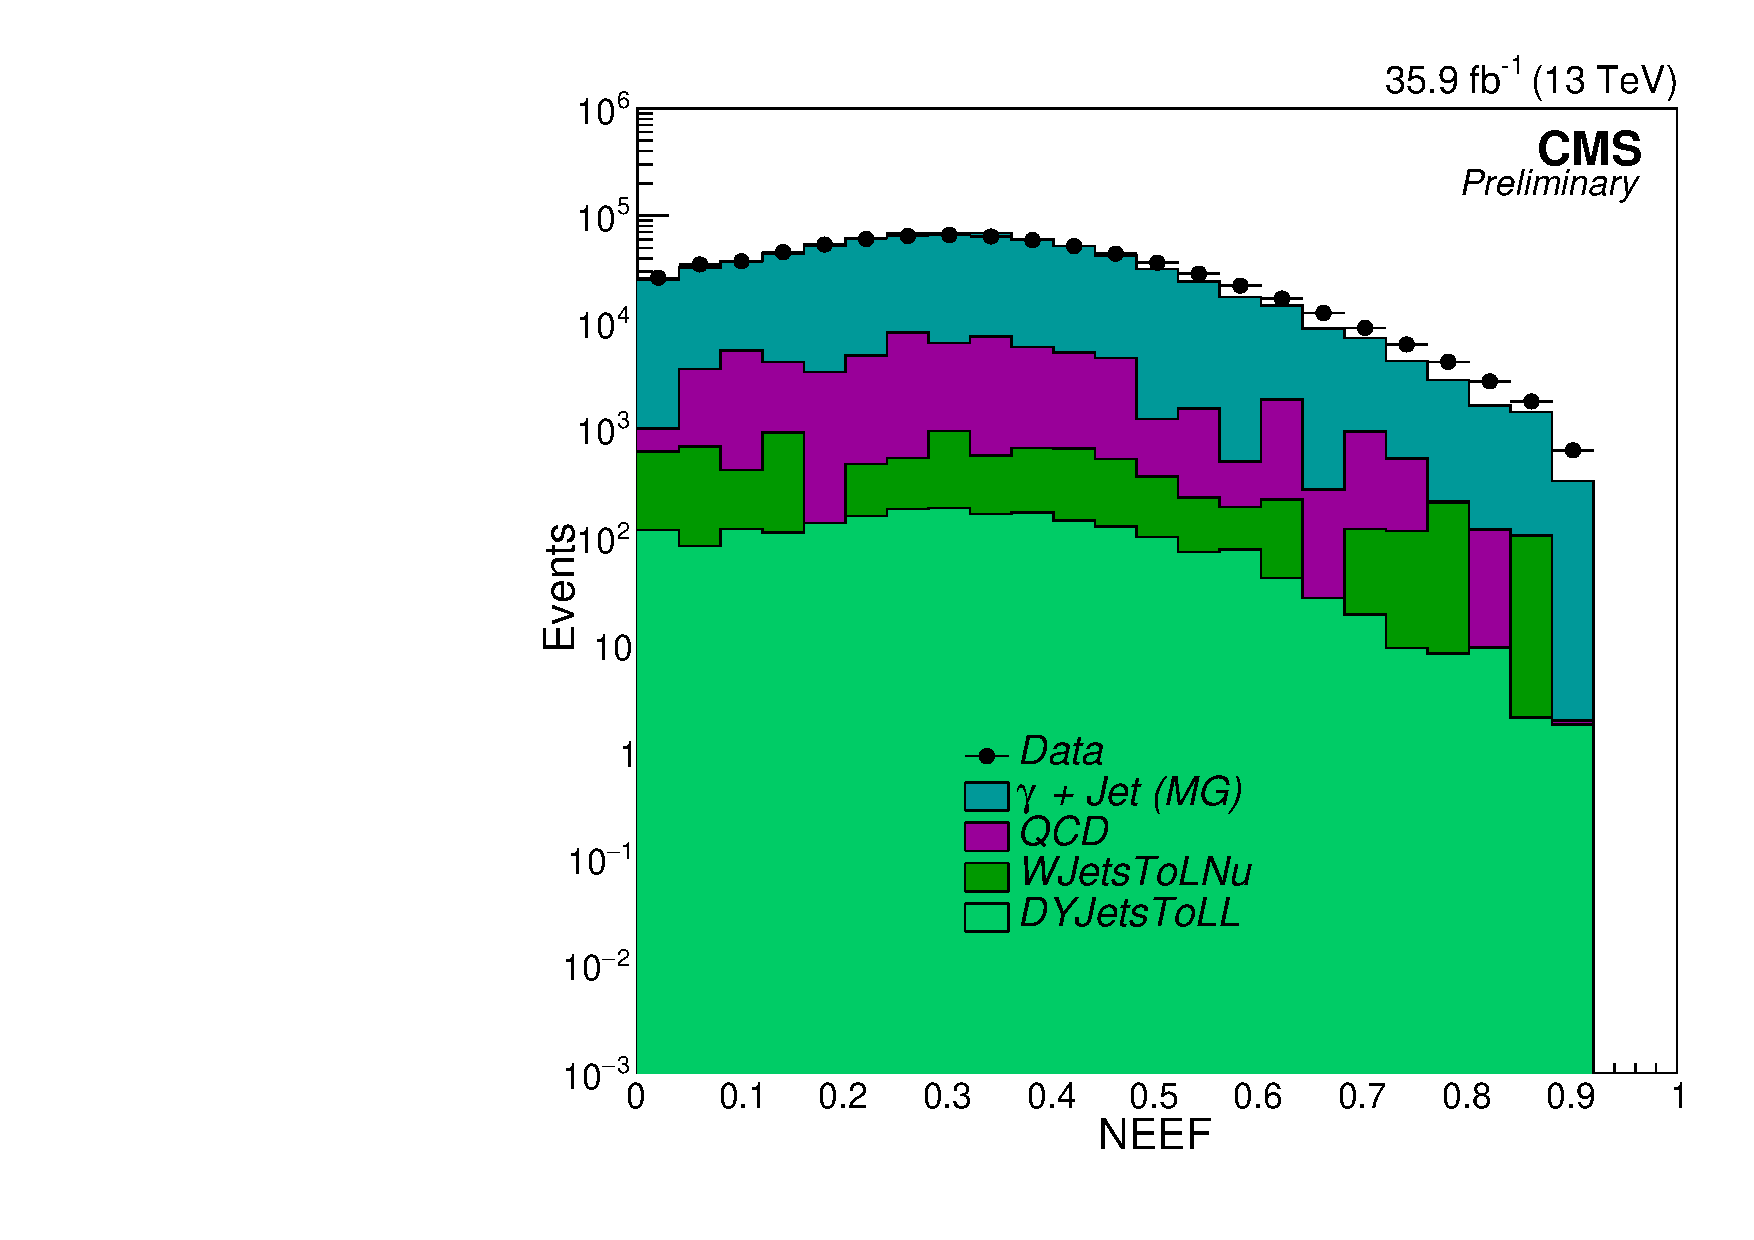
\includegraphics[width=7cm]{Chapter4/JetID/Jet_NEEF.pdf}} \hspace{0.2in}
\subfloat[Charged EM Energy Fraction]{\label{fig:Jet_CEEF}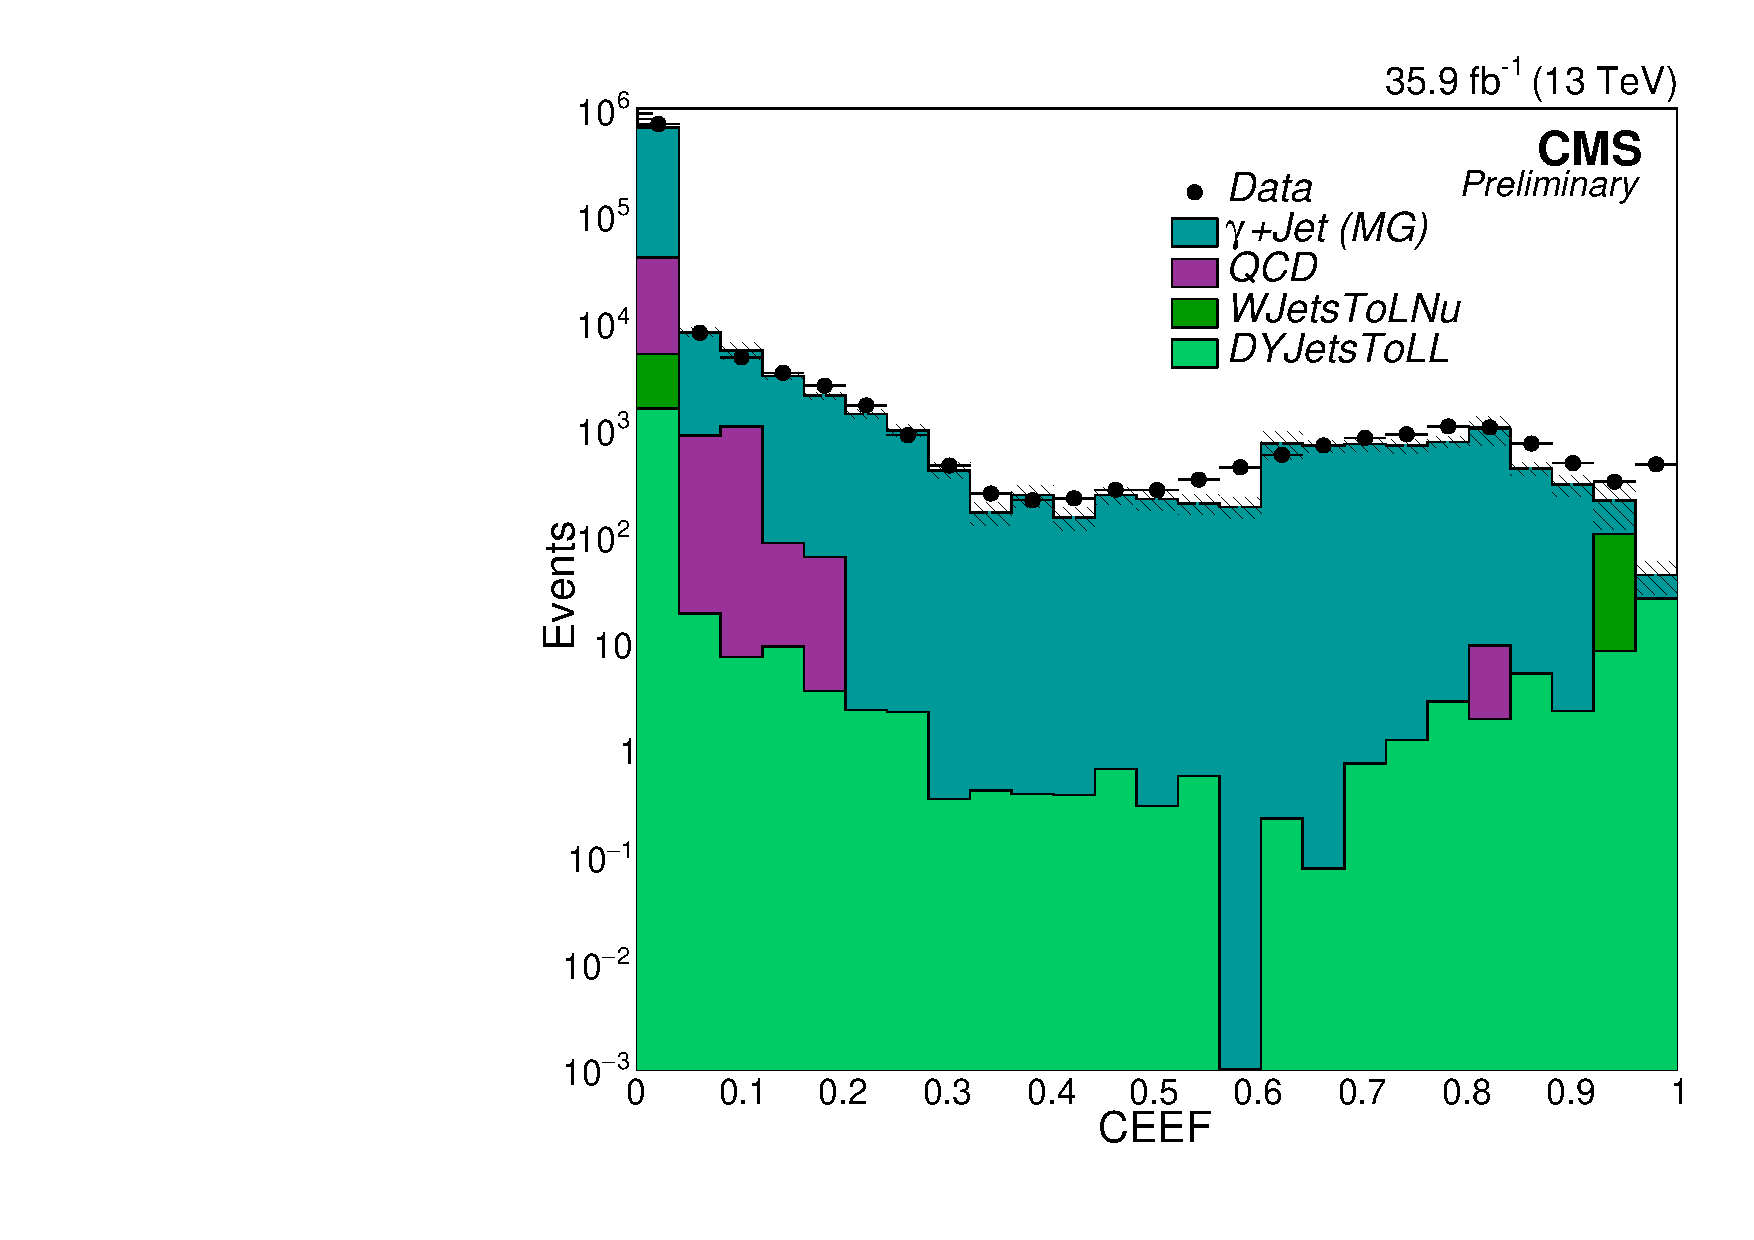
\includegraphics[width=7cm]{Chapter4/JetID/Jet_CEEF.pdf}}   \\
\subfloat[Number of Constituents]{\label{fig:Jet_NConst}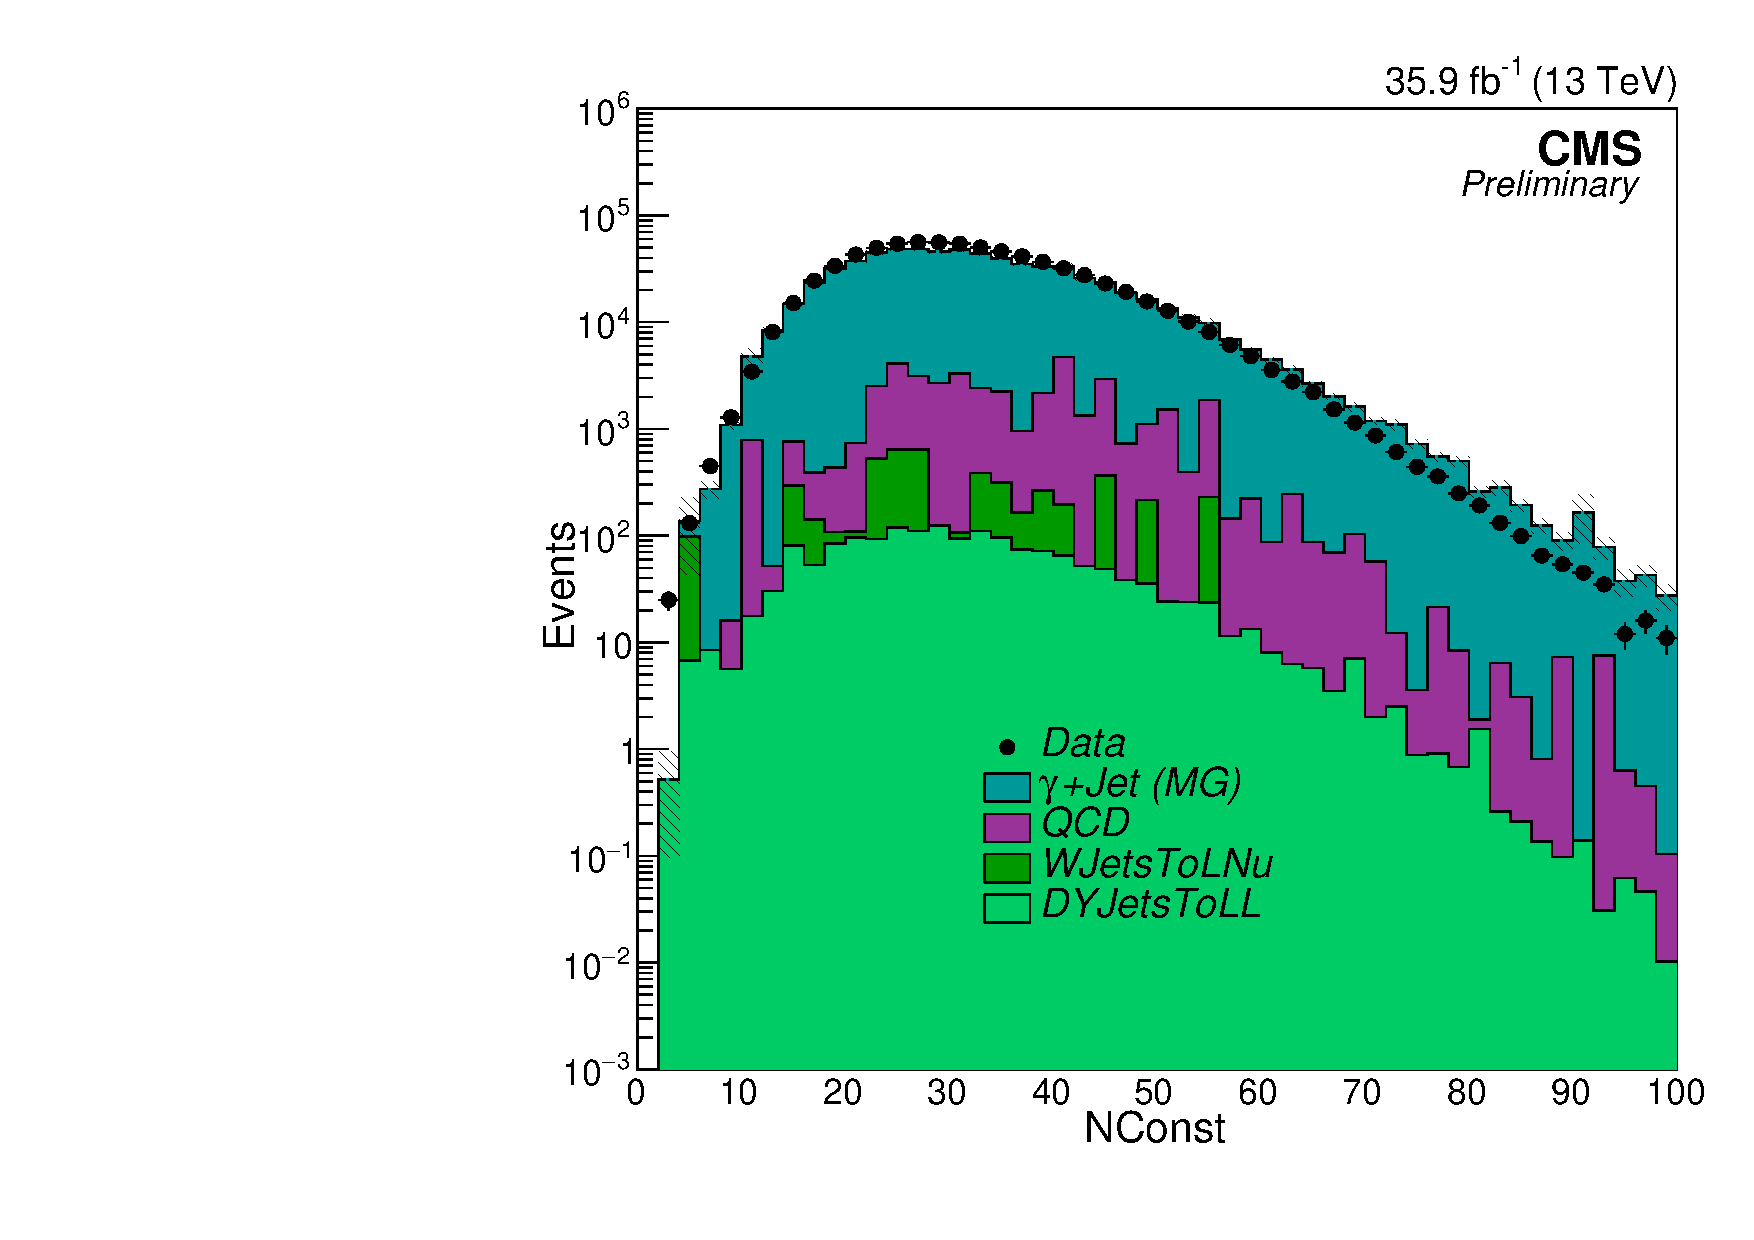
\includegraphics[width=7cm]{Chapter4/JetID/Jet_NConst.pdf}} \hspace{0.2in}
\subfloat[Charged Multiplicity]{\label{fig:Jet_ChMult}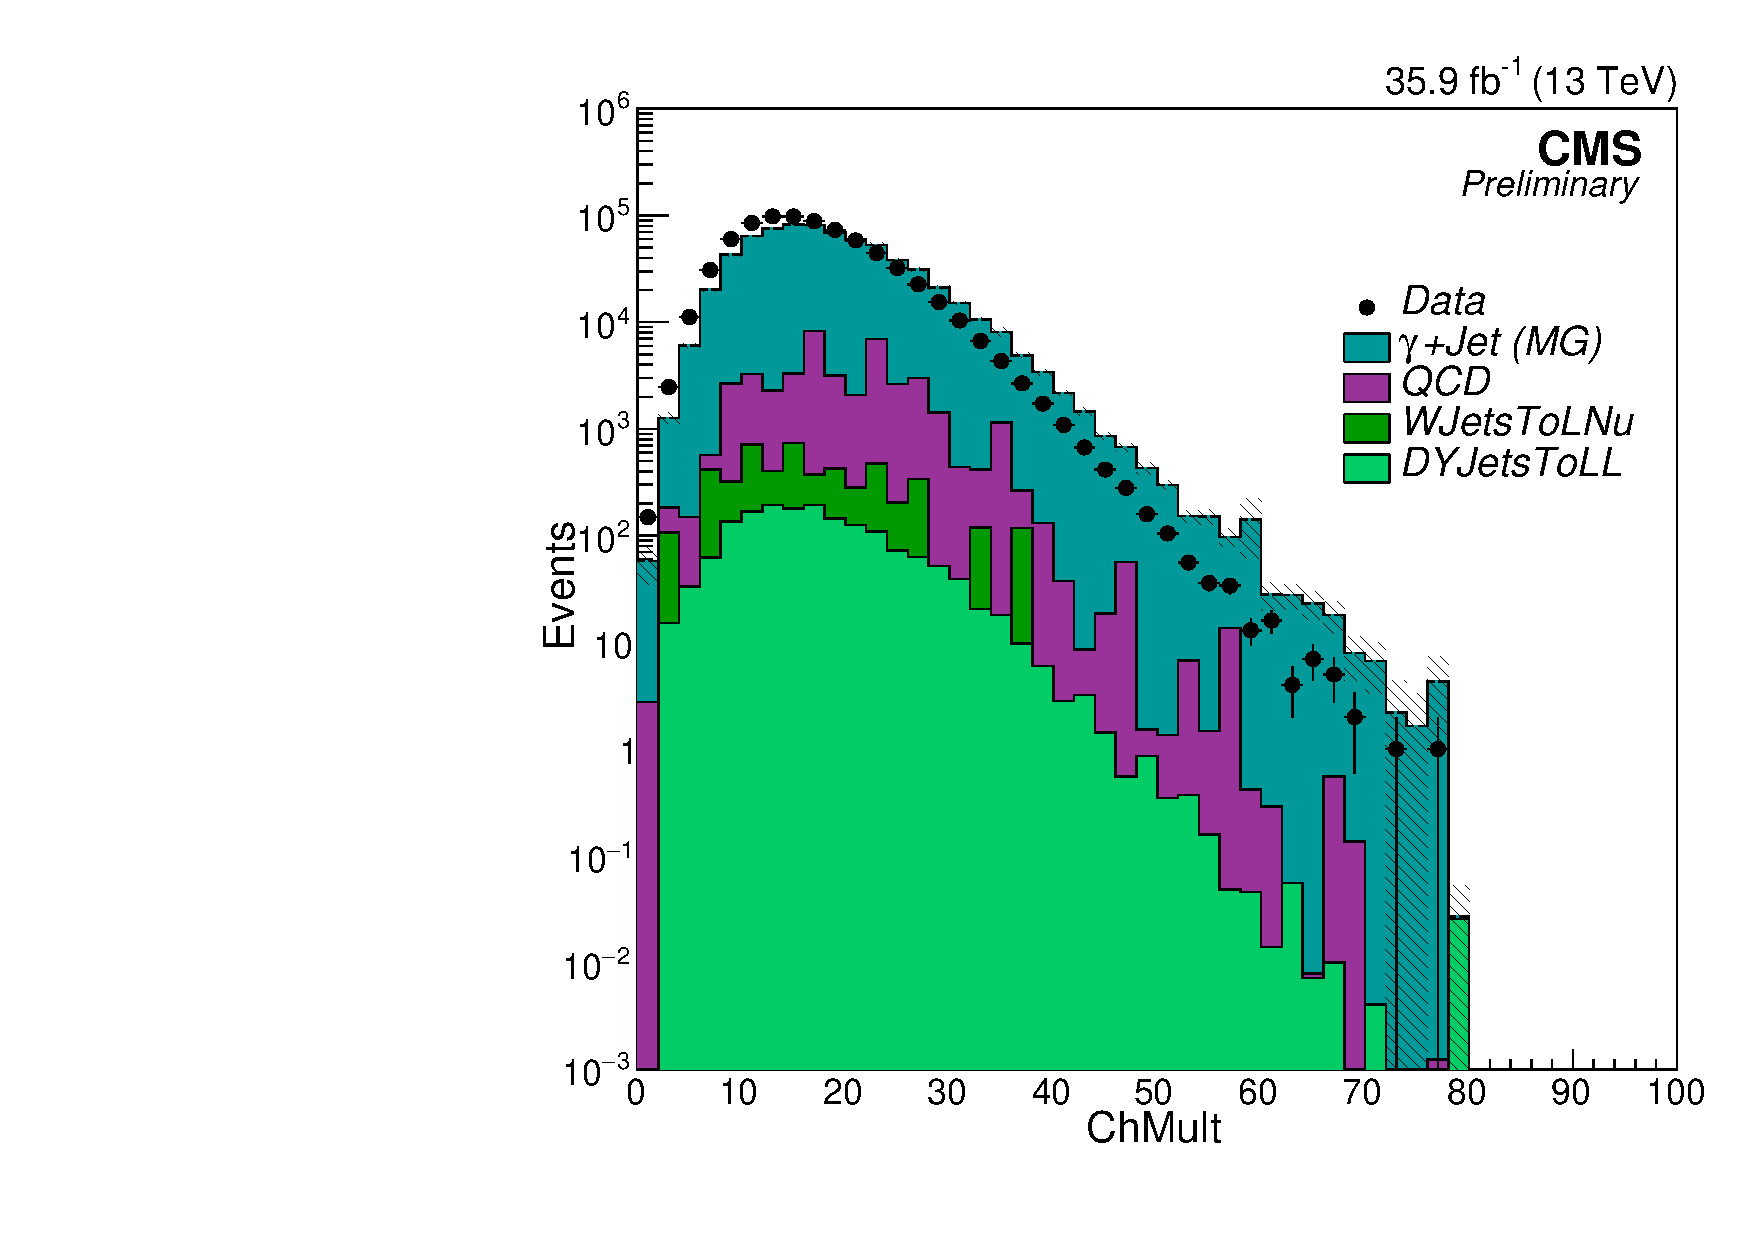
\includegraphics[width=7cm]{Chapter4/JetID/Jet_ChMult.pdf}}
\caption{Data-MC comparison of jet particle flow identification variables after final selection.}
\label{fig:JetId}
\end{figure}

\subsection{Analysis object selection: b-Jet}
The selected jet in each event is examined for its b-tagging status using the ``CSVv2'' (explained in \sectn{\ref{Se:Jet_btagging}})
discriminator. A cut-off value of 0.5426, corresponding to the loose working point, has been used and all the jets with b-tag discriminator
value greater than the cut-off value are considered as b-jets.

In general, the b-jet identification efficiency and c$/$light-jet misidentification probability of a tagger is not the same in data and MC. These observed differences
are taken into account by means of the b-tag scale factors (SF) defined as, SF = $\frac{\epsilon_{\textrm{data}}}{\epsilon_{\textrm{MC}}}$, where
$\epsilon_{\textrm{data}}$ and $\epsilon_{\textrm{MC}}$ are the b-tagging efficiencies of CSVv2 discriminator in data and MC simulation, respectively. These
SFs, in CMS, are determined using the dedicated techniques, described in~\cite{Chatrchyan:2012jua, Sirunyan:2017ezt}.
The SFs are dependent on jet flavor, jet \pt and jet $\eta$.
The official recommendations for computing these scale factors and errors on them are provided
in~\cite{Web:BtagReco}. The SFs are available for the \pt range of 20$-$1000\unit{GeV}
and $|\eta|$ $<$ 2.4. For values above the \pt limit, the recommendations are to use the SF values at the limits with double the uncertainty
while for values above the $\eta$ limits, the SF values are taken equal to zero.

Errors on b-tag scale factors arise from various systematic uncertainties, like the jet energy scale uncertainty, the sample purity which is
the contamination of jets with a flavor complementary to the one for which the scale factor is being measured, the uncertainty on the scale factor for
c-jets and the uncertainty due to finite number of events in the simulation which results into statistical fluctuations etc.
These errors are evaluated as the differences in the scale factors for central and up$/$down systematic type as mentioned in~\cite{Web:BtagReco}
and are used as a source of systematic uncertainty due to the b-tagging.

In principle, the SF value provides the fraction of actual b-jets among the jets passing the discriminator cut. Based on this terminology, two b-tag categories are
formed:
\vspace{-0.1in}
\begin{itemize}[leftmargin=*]
\item 1 b-tag category $=$ Jets passing the discriminator $\times$ SF.
\item 0 b-tag category $=$ Jets passing the discriminator $\times$ (1 $-$ SF) $+$ Jets failing the discriminator.
\end{itemize}
\vspace{-0.1in}
So the 1 b-tag category essentially gives the fraction of b-jets and the 0 b-tag category gives the fraction of non b-jets, called as the 1 and 0 b-tag
efficiencies of discriminator. A Data-MC comparison of the CSVv2 discriminator before and after applying the b-tagging is shown in \fig{\ref{fig:CSVv2_dist}}.
The 0 b-tag category may contain the jets passing the discriminator, with a weight (1 $-$ SF), as is seen in \fig{\ref{fig:CSVv2_0}}.

\begin{figure}[h!]
\centering
\subfloat[no b-tag]{\label{fig:CSVv2_no}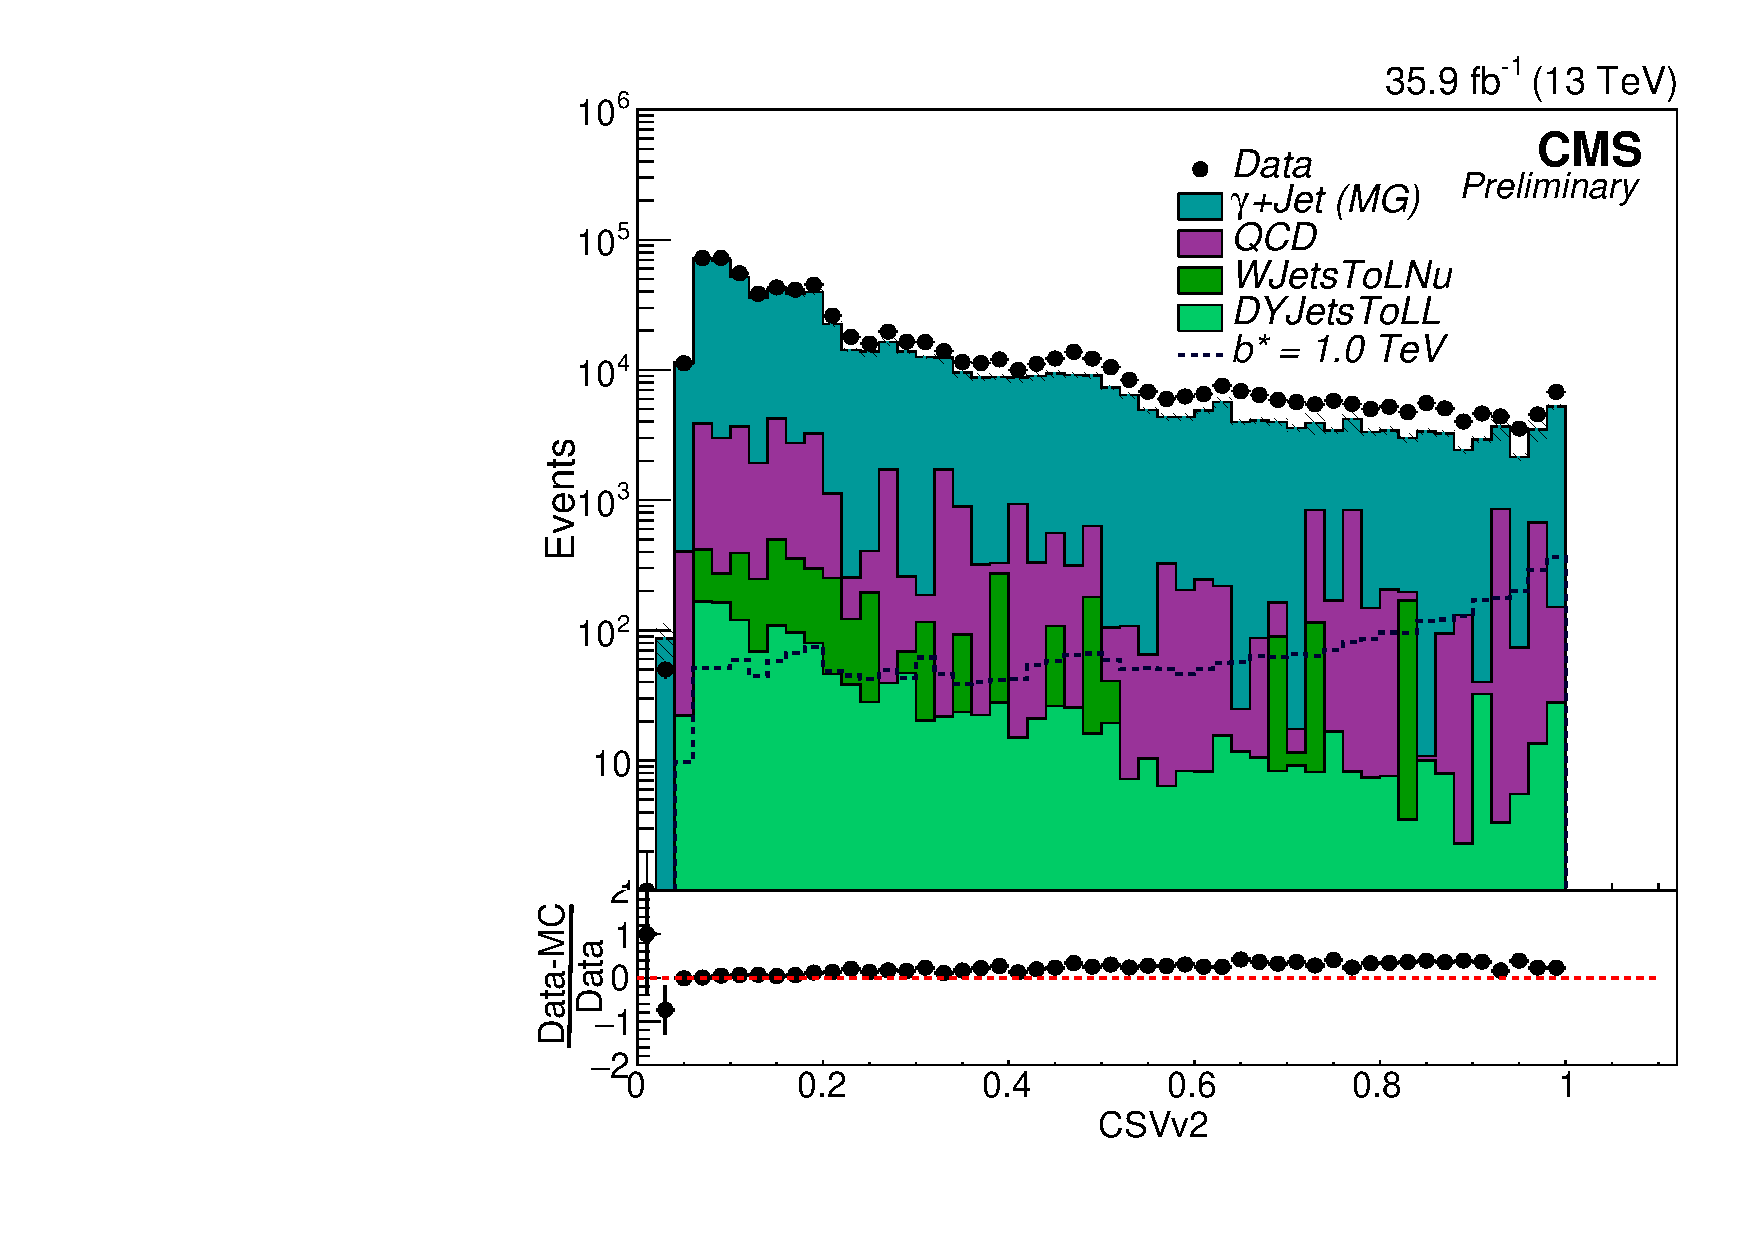
\includegraphics[width=5.3cm]{Chapter4/CSVv2_Dist/CSV_no.pdf}}
\subfloat[0 b-tag]{\label{fig:CSVv2_0}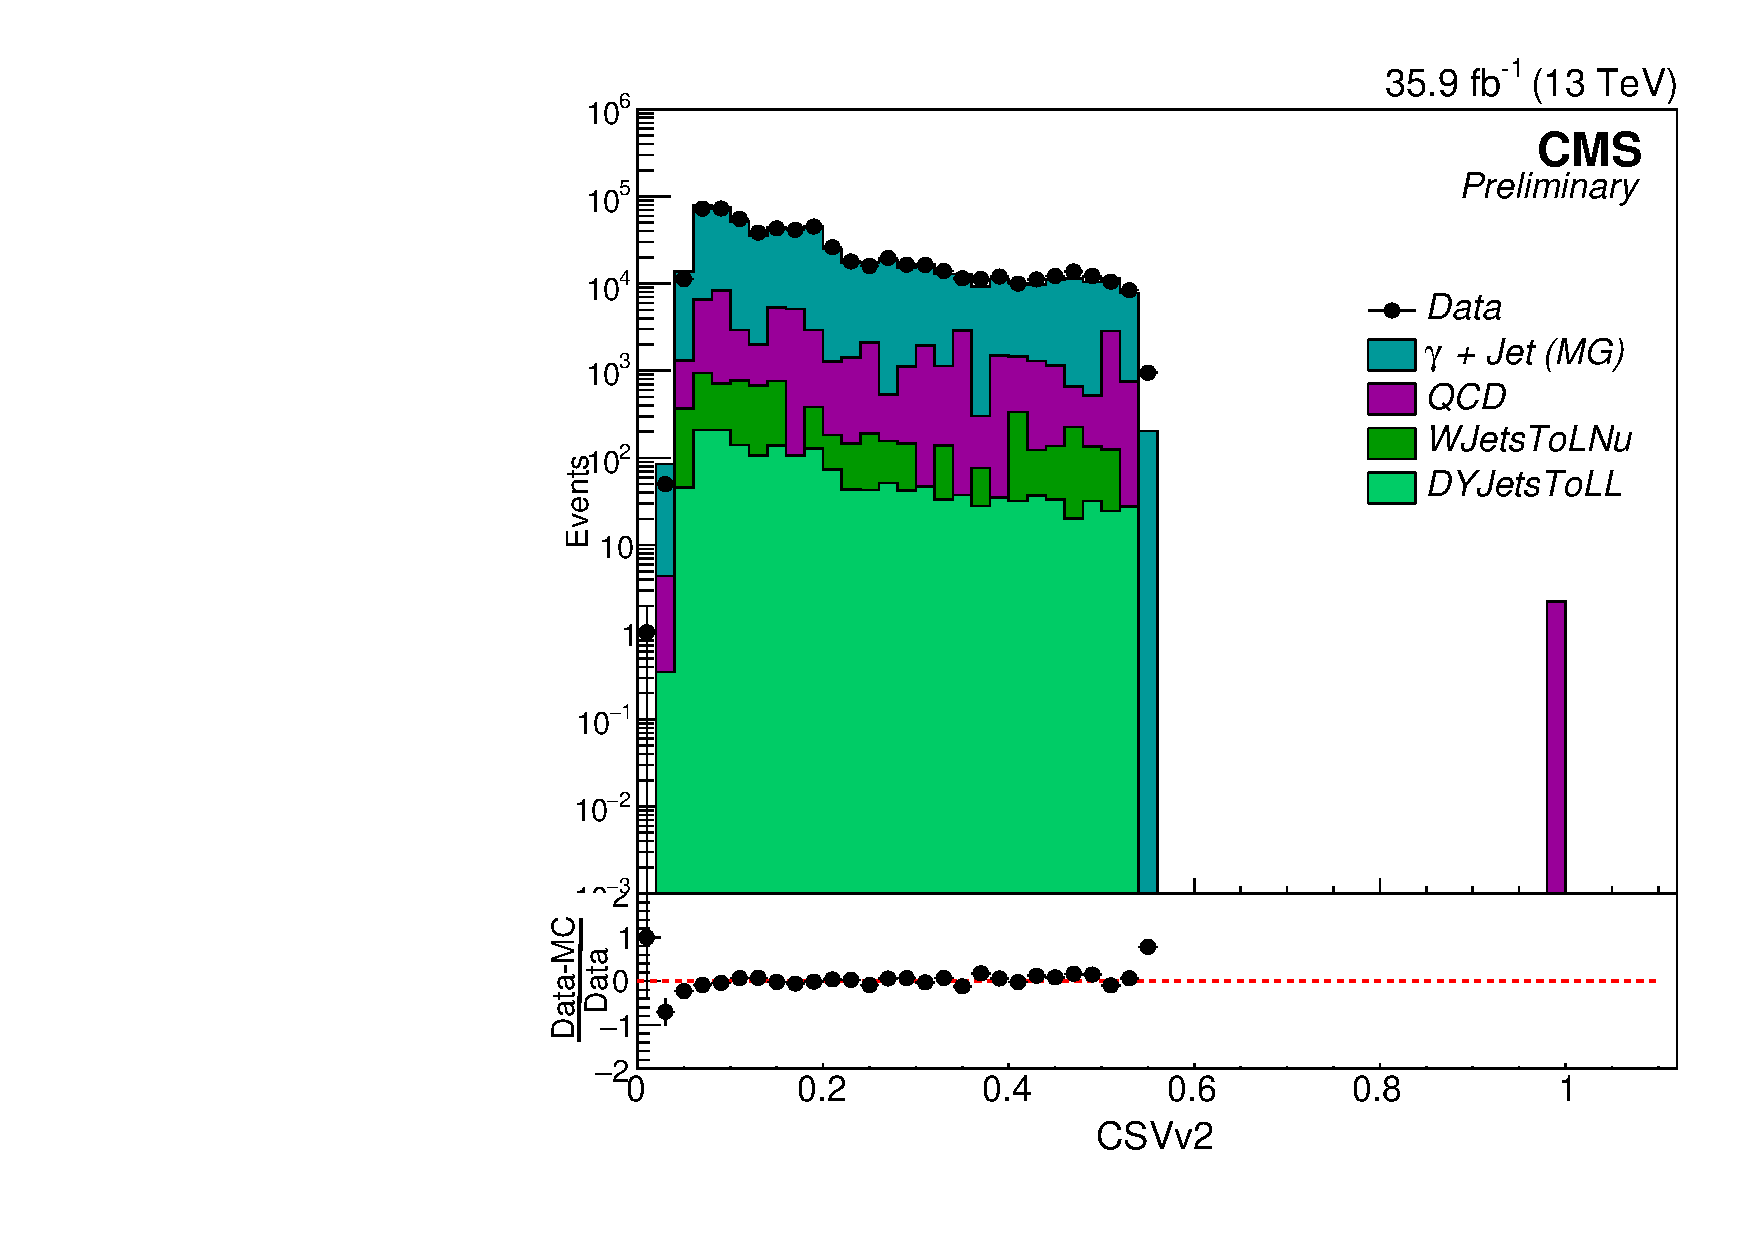
\includegraphics[width=5.3cm]{Chapter4/CSVv2_Dist/CSV_0.pdf}} 
\subfloat[1 b-tag]{\label{fig:CSVv2_1}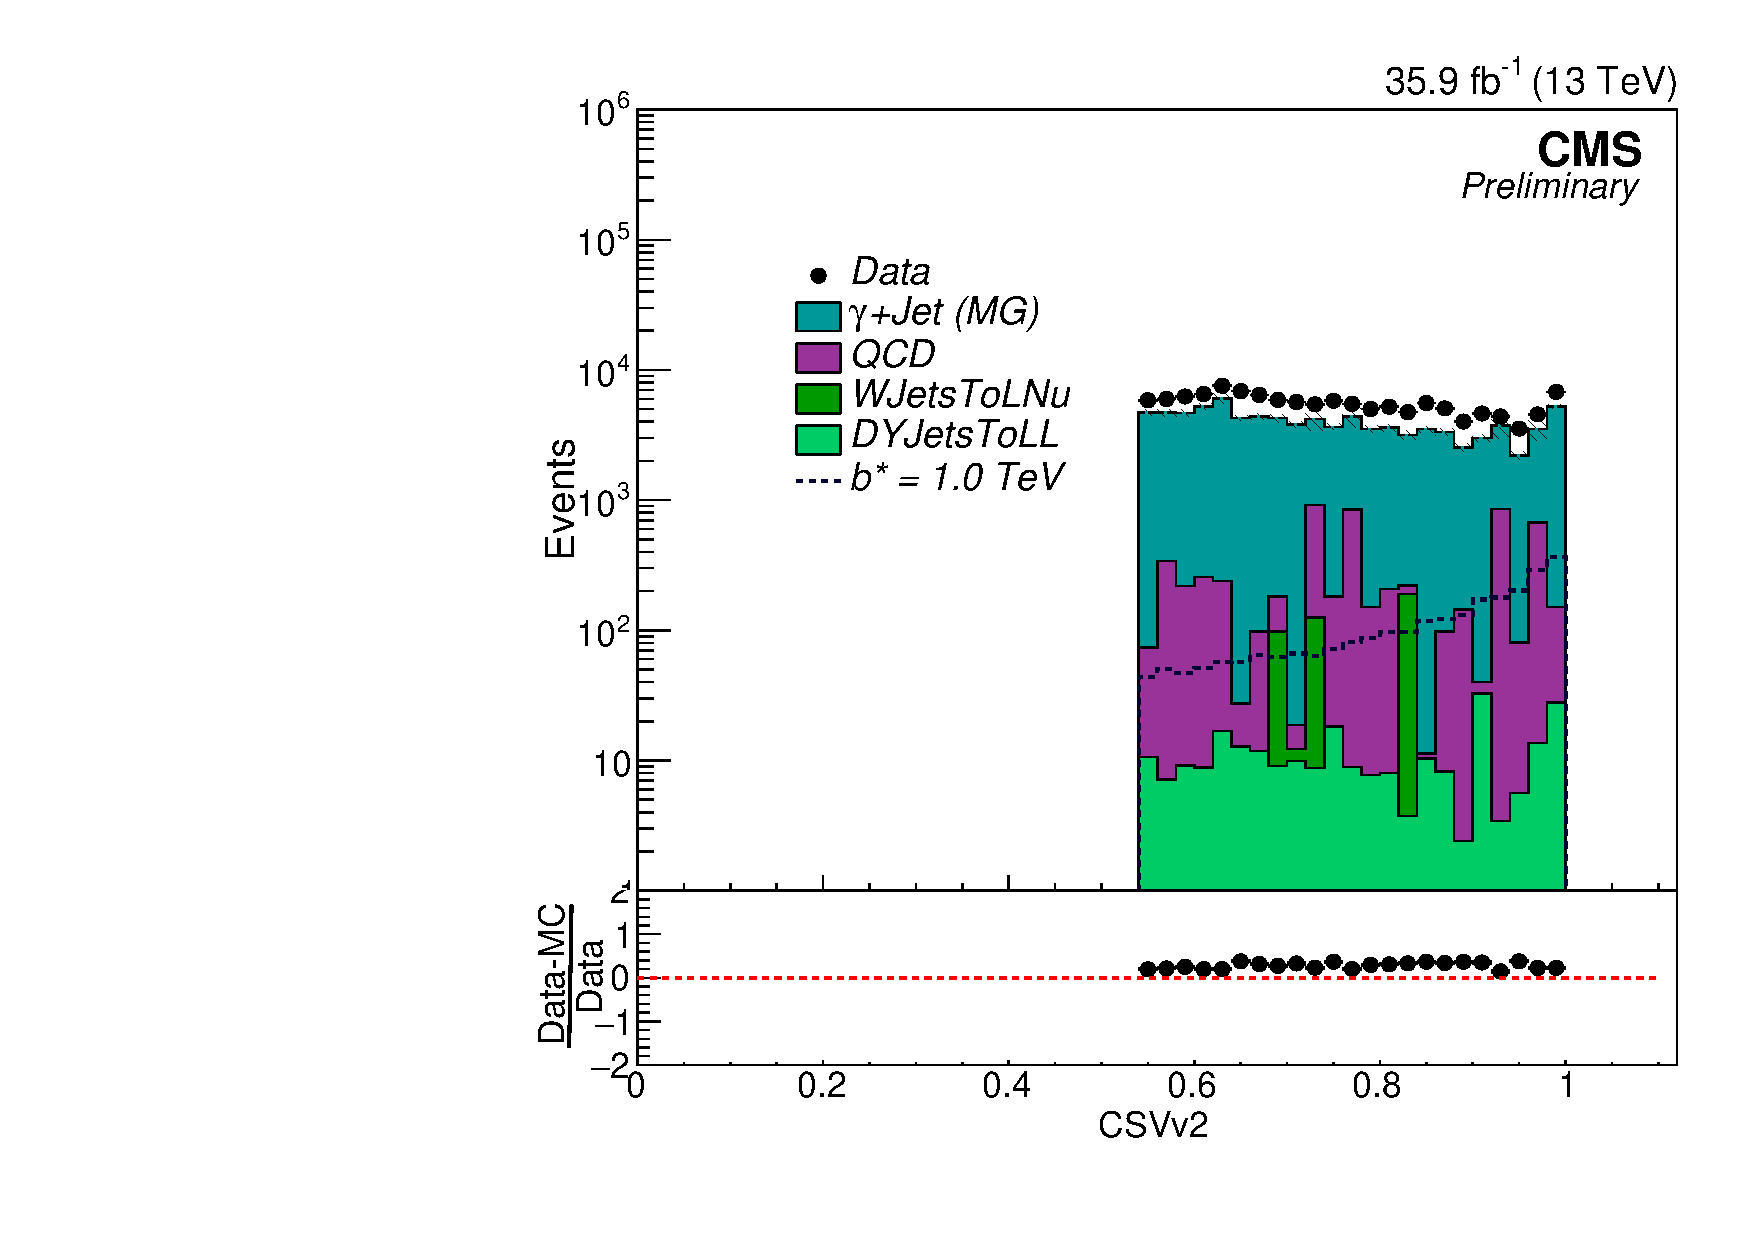
\includegraphics[width=5.3cm]{Chapter4/CSVv2_Dist/CSV_1.pdf}} 
\caption{Data-MC comparison of CSVv2 discriminator distribution before and after applying the b-tagging.}
\label{fig:CSVv2_dist}
\end{figure}

\subsection{Kinematical restrictions between $\gamma$ and jet$/$b-jet}
The $\gamjet$ final state from excited quark decays would be produced through a s-channel process and has an isotropic distribution of final state particles.
On the other hand, the $\gamjet$ final state from background processes would take place through a t-channel process and result into high density of particles
in forward and backward directions. Hence, to reduce these background contributions while maintaining high acceptance for the signal, 
$|\Delta\eta(\gamma, \textrm{jet}/\textrm{b-jet})|$ $<$ 1.5 has been applied. Also, in order to avoid the turn-on region due to various kinematical selections,
as shown in \fig{\ref{fig:MassTurnOn}}, a cut on the invariant mass of $\gamjet/$b-jet,
M$_{\gamjet}$ = $\sqrt{(\textrm{E}^{\gamma} + \textrm{E}^{\textrm{jet}})^{2} - (\vec{\textrm{p}}^{\gamma} + \vec{\textrm{p}}^{\textrm{jet}})^{2}}$,
has been applied and is required to be greater than 700\unit{GeV}.

\begin{figure}[h!]
\centering
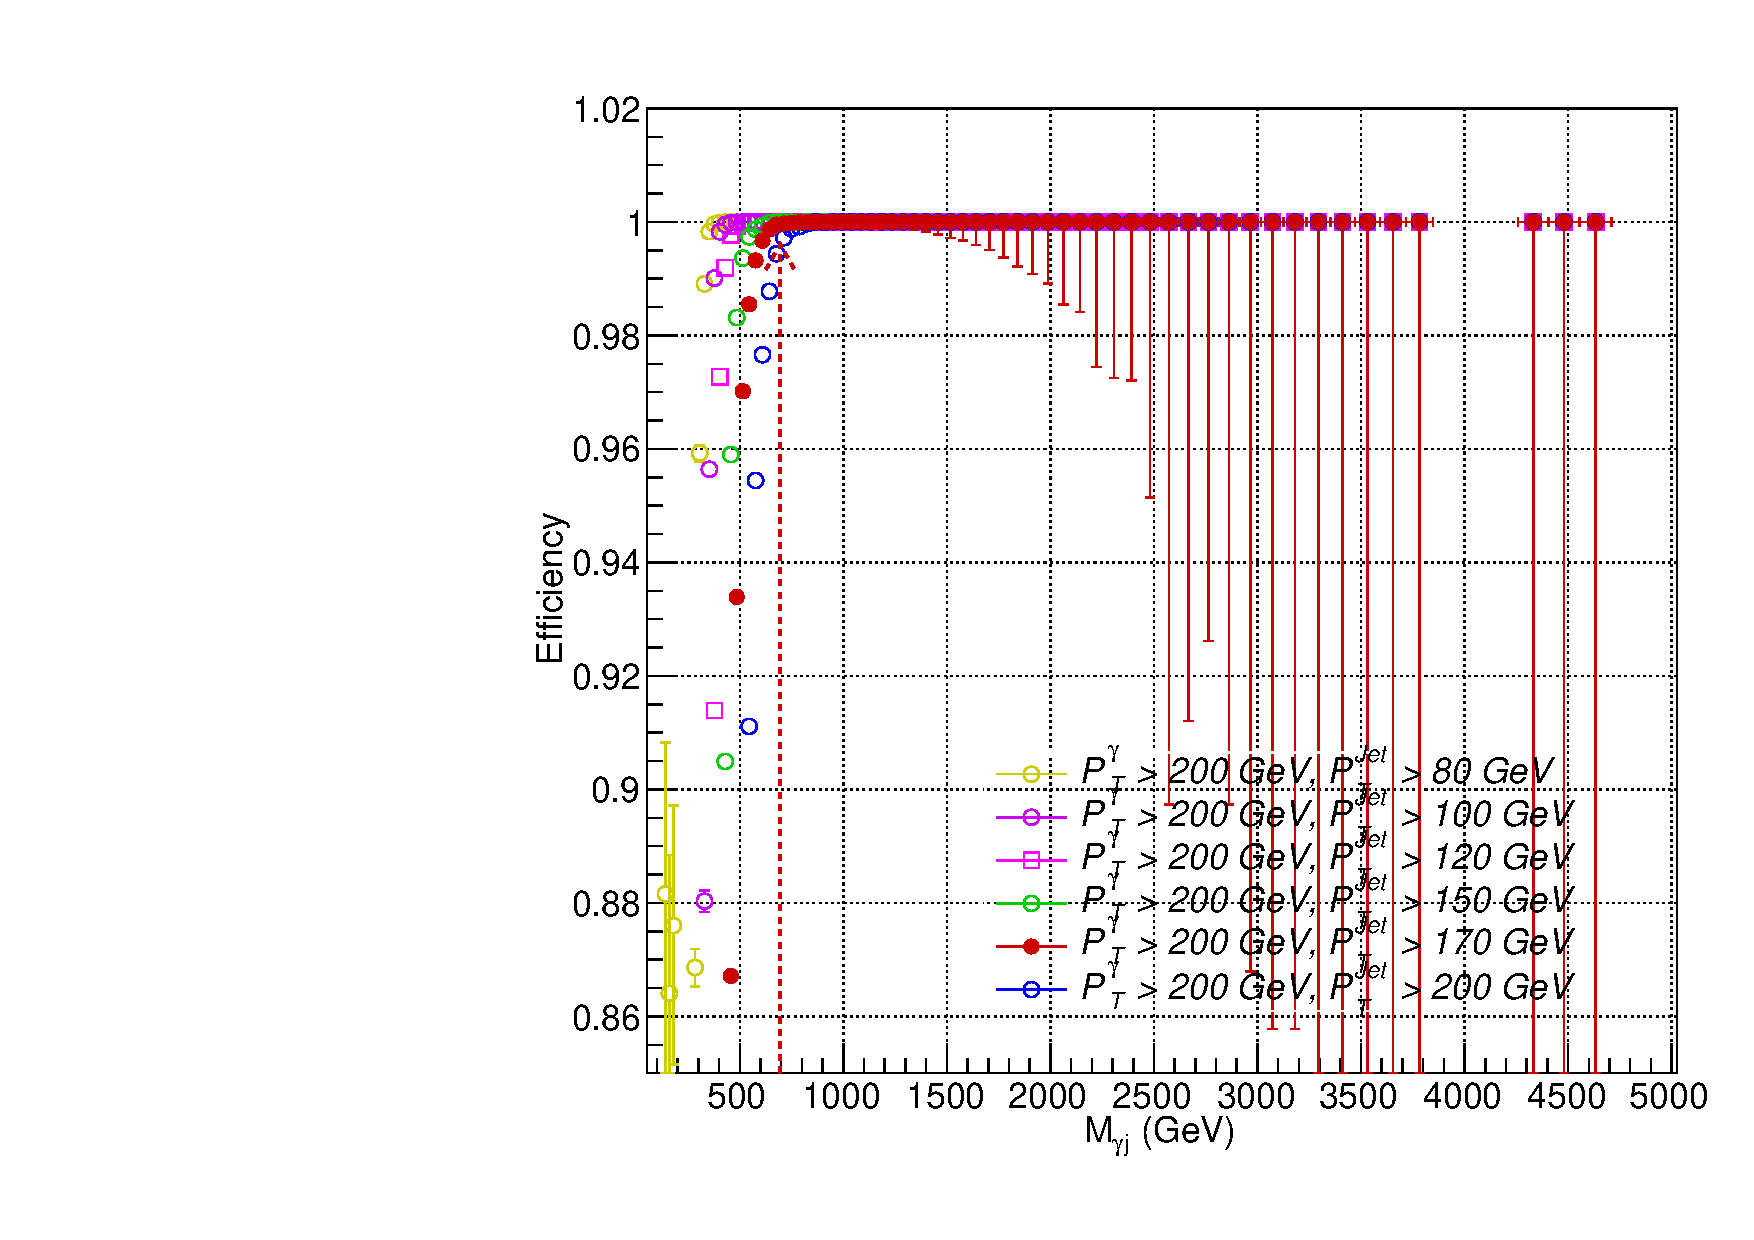
\includegraphics[width=9.5cm]{Chapter4/MassTurnOn/MassTurnOn_afterfinalselection.pdf}
\caption{Turn-on due to various kinematical selections, plotted for different jet \pt cuts.}
\label{fig:MassTurnOn}
\end{figure}

The theoretical predictions for $\gamjet$ and dijet backgrounds are generated at the LO level using \pythia and \madgraph, so in order to include the NLO effects,
the MC events are scaled with a K-factor of 1.3~\cite{dijetkfactor1, dijetkfactor2}, along with the luminosity and pile-up scale factors.
The cut flow table for signal, backgrounds and data, after application of all selection cuts and scale factors, is presented in \tab{\ref{Table:SelCutFlow}}.
The SM $\gamjet$ contributes about 95$\%$ of the total background while the contribution from
QCD dijet background is around 4$\%$ and from electroweak background is around 1$\%$. 

\begin{table}[htbp]
  \begin{center}
    \resizebox{16cm}{!}{
      \begin{tabular}{lcccccc}
        \toprule
        \belowrulesepcolor{Mygray}
        \belowrulesepcolor{Mygray}
        \belowrulesepcolor{Mygray}
        \rowcolor{Mygray}[\dimexpr\tabcolsep+0.09pt\relax]
        \bf {Cuts}  &  \bf {\bf{\qstar} 2\unit{\bf{TeV}}}    &  \bf {SM $\gamjet$ Bkg}  &  \bf {QCD dijet Bkg}  &  \bf {EWK Bkg}  &  \bf {Total Bkg}  &  \bf {Data}\\
        \aboverulesepcolor{Mygray}
        \aboverulesepcolor{Mygray}
        \aboverulesepcolor{Mygray}
        \midrule
        Total                           &  18389.6  &    1.50357E$+$09 &  2.66074E$+$10 &  2.87352E$+$09 &  3.09845E$+$10    & 1.1584E$+$08 \\
        HLT                             &  18389.6  &    1.50357E$+$09 &  2.66074E$+$10 &  2.87352E$+$09 &  3.09845E$+$10    & 3.93895E$+$07 \\
        MET filters                      &  18389.6  &    1.50357E$+$09 &  2.66074E$+$10 &  2.87352E$+$09 &  3.09845E$+$10    & 3.74467E$+$07 \\ 
        Photon ID                &  12868.4  &    6.38738E$+$08 &  6.70708E$+$07 &  7.31732E$+$07 &  7.78982E$+$08    & 4.20307E$+$06 \\   
        $\pt^{\gamma}$ $>$ 200\unit{GeV} \& &  11552.4  &    1.06063E$+$06 &  481691      &  9231.4      &  1.55155E$+$06    & 1.26456E$+$06 \\   
        $|{\eta}^{\gamma}|$ $<$ 1.4442  &           &                &              &              &                 &              \\
        QCD overlap removal             &  11552.4  &    1.06007E$+$06 &  91298.3     &  9231.4      &  1.1606E$+$06     & 1.26456E$+$06  \\
        Jet ID                    &  11548.1  &    1.05854E$+$06 &  91244.5     &  8953.46     &  1.15874E$+$06    & 1.26033E$+$06 \\ 
        $\pt^{\textrm{jet}}$ $>$ 170\unit{GeV}       &  11496.6  &    814187      &  74359.6     &  6393.9      &  894940         & 930191 \\
        $|{\eta}^{\textrm{jet}}|$ $<$ 2.4        &    11193  &    782291      &  62086.8     &  6179.82     &  850558         & 905346 \\      
        $|\Delta\eta|$ $<$ 1.5                &  8270.48  &    652420      &  37343.4     &  5201.72     &  694965         & 748663 \\  
        M$_{\gamjet}$ $>$ 700\unit{GeV}                &  8237.03  &    122831      &  4950.45     &  1379.37     &  129160         & 126770 \\
        \bottomrule
      \end{tabular}
    }
    \caption{Selection cut flow table for signal, different backgrounds and data.}
    \label{Table:SelCutFlow}
  \end{center}
\end{table}

\begin{table}[htbp]
  \begin{center}
    \resizebox{15cm}{!}{
      \begin{tabular}{lccccccc}
        \toprule
        \belowrulesepcolor{Mygray}
        \belowrulesepcolor{Mygray}
        \belowrulesepcolor{Mygray}
        \rowcolor{Mygray}[\dimexpr\tabcolsep+0.09pt\relax]
        \bf {Cuts} & \bf {1\unit{\bf{TeV}}} & \bf {2\unit{\bf{TeV}}} & \bf {3\unit{\bf{TeV}}} & \bf {4\unit{\bf{TeV}}} & \bf {5\unit{\bf{TeV}}} & \bf {6\unit{\bf{TeV}}}  &  \bf {7\unit{\bf{TeV}}} \\
        \aboverulesepcolor{Mygray}
        \aboverulesepcolor{Mygray}
        \aboverulesepcolor{Mygray}
        \midrule
        Total                           &   100   &  100   &  100   &  100   &  100   &  100   &  100   \\
        Photon ID                &    69.4811  &     69.3168  &      69.696  &     70.0057  &     70.2649  &     69.0685  &     67.0689    \\ 
        $\pt^{\gamma}$ $>$ 200\unit{GeV} \& &    54.6384  &     62.2149  &     63.6378  &     64.1612  &     64.5831  &     63.3158  &     61.0851    \\
        $|{\eta}^{\gamma}|$ $<$ 1.4442 &    &       &       &       &       &       &           \\
        Jet ID                    &    54.5833  &     62.1878  &     63.6138  &      64.149  &     64.5657  &     63.3051  &     61.0571    \\ 
        $\pt^{\textrm{jet}}$ $>$ 170\unit{GeV}   &    53.1439  &     61.9043  &     63.5149  &     64.0551  &     64.4989  &     63.2264  &      60.977    \\
        $|{\eta}^{\textrm{jet}}|$ $<$ 2.4       &    50.0591  &     60.2276  &     62.7361  &     63.6412  &     64.2839  &      63.061  &     60.7929    \\
        $|\Delta\eta|$ $<$ 1.5     &    39.2106  &        44.5  &     45.5168  &     45.5196  &     45.7801  &     44.6649  &     43.2637    \\
        M$_{\gamjet}$ $>$ 700\unit{GeV}   &    37.4718  &      44.317  &     45.4661  &      45.472  &     45.7347  &     44.6102  &     43.2077    \\ 
        \bottomrule
      \end{tabular}
    }
    \caption{Selection efficiency ($\%$) table for the \qstar signal samples in the mass range 1.0$-$7.0\unit{TeV} with SM Coupling $f$ $=$ 1.0.}
    \label{Table:SelEff_Qstarf1p0}
  \end{center}
\end{table}

\begin{table}[htbp]
  \begin{center}
    \resizebox{15cm}{!}{
      \begin{tabular}{lccccccc}
        \toprule
        \belowrulesepcolor{Mygray}
        \belowrulesepcolor{Mygray}
        \belowrulesepcolor{Mygray}
        \rowcolor{Mygray}[\dimexpr\tabcolsep+0.09pt\relax]
        \bf {Cuts}  &  \bf {1\unit{\bf{TeV}}}  &  \bf {1.5\unit{\bf{TeV}}}  &  \bf {2\unit{\bf{TeV}}}  &  \bf {2.5\unit{\bf{TeV}}}  &  \bf {3\unit{\bf{TeV}}}  &  \bf {3.5\unit{\bf{TeV}}}  &  \bf {4\unit{\bf{TeV}}} \\
        \aboverulesepcolor{Mygray}
        \aboverulesepcolor{Mygray}
        \aboverulesepcolor{Mygray}
        \midrule
        Total                          &       100  &         100  &         100  &         100  &         100  &         100  &         100    \\ 
        Photon ID                &     69.8006  &     69.6057  &     69.8508  &     70.3567  &     70.4957  &     71.1226  &     70.9883    \\ 
        $\pt^{\gamma}$ $>$ 200\unit{GeV} \& &     54.6467  &     58.3353  &     60.0603  &     61.3592  &     62.1837  &     62.5457  &     63.0047    \\ 
        $|{\eta}^{\gamma}|$ $<$ 1.4442  &    &       &       &       &       &       &             \\
        Jet ID                    &     54.6361  &     58.3307  &     60.0561  &     61.3549  &     62.1784  &     62.5411  &     62.9972    \\ 
        $\pt^{\textrm{jet}}$ $>$ 170\unit{GeV}   &     53.1637  &     57.8604  &     59.8709  &     61.2866  &     62.1325  &     62.4845  &     62.9699    \\ 
        $|{\eta}^{\textrm{jet}}|$ $<$ 2.4    &     52.5537  &     57.3699  &     59.4802  &     61.0701  &      61.952  &     62.4065  &     62.9059    \\ 
        CSVv2             &     35.5183  &     35.6018  &     34.2311  &     30.9516  &      28.901  &     28.1197  &     27.3777    \\ 
        $|\Delta\eta|$ $<$ 1.5    &     28.4642  &     26.5476  &     25.3583  &     22.5024  &     20.4847  &     19.8818  &     19.5085    \\
        M$_{\gamjet}$ $>$ 700\unit{GeV}     &     27.3834  &     26.4028  &     25.3119  &     22.4633  &     20.4636  &     19.8627  &     19.4598    \\ 
        \bottomrule
      \end{tabular}
    }
    \caption{Selection efficiency ($\%$) table for the \bstar signal samples in the mass range 1.0$-$4.0\unit{TeV} with SM Coupling $f$ $=$ 1.0.}
    \label{Table:SelEff_Bstarf1p0}
  \end{center}
\end{table}

%\begin{table}[h!]
%\begin{center}
%\begin{tabular}{|l|c|c|c|c|c|c|c|c|c|c|}
%\hline
%{\bf Cuts}  &  {\bf 500}  &  {\bf 1000}  &  {\bf 1500}  &  {\bf 2000}  &  {\bf 2500}  &  {\bf 3000}  &  {\bf 3500}  &  {\bf 4000}  &  {\bf 4500}  & % {\bf 5000} \\
%\hline
%Total                           &  100  &  100  &  100  &  100  &  100  &  100  &  100  &  100  &  100  &  100  \\
%loose PhotonID                  & 79.9  & 80.5  & 80.9  & 80.6  & 80.1  & 81.3  & 80.1  & 82.0  & 81.1  & 81.3   \\
%P$_{T}^{\gamma}$ $>$ 190 GeV \& & 41.5  & 63.3  & 67.8  & 69.1  & 71.0  & 71.7  & 71.8  & 73.2  & 72.7  & 73.1    \\
%$|{\eta}^{\gamma}|$ $<$ 1.4442  &       &       &       &       &       &       &      &        &       &         \\ 
%Tight JetID                     & 41.5  & 63.3  & 67.8  & 69.1  & 71.0  & 71.7  & 71.8  & 73.2  & 72.7  & 73.1    \\
%P$_{T}^{Jet}$ $>$ 190 GeV       & 27.1  & 60.6  & 67.1  & 68.9  & 70.9  & 71.6  & 71.7  & 73.2  & 72.7  & 73.1    \\
%$|{\eta}^{Jet}|$ $<$ 2.4        & 26.9  & 60.1  & 66.5  & 68.6  & 70.7  & 71.5  & 71.7  & 73.2  & 72.7  & 73.1    \\
%${\Delta}{\phi}$ $>$ 2.5        & 24.3  & 55.8  & 63.1  & 66.1  & 68.6  & 69.9  & 70.4  & 72.4  & 72.0  & 72.2    \\
%$|{\Delta}{\eta}|$ $<$ 2.2      & 24.1  & 51.9  & 56.7  & 58.9  & 60.7  & 61.8  & 62.0  & 63.3  & 63.0  & 63.2    \\
%Mass $>$ 695 GeV                &  1.4  & 50.4  & 56.6  & 58.9  & 60.7  & 61.8  & 62.0  & 63.3  & 63.0  & 63.2    \\
%CSVv2M                          & 13.5  & 23.6  & 19.1  & 14.3  & 11.1  &  9.4  &  8.6  &  8.2  &  8.0  &  8.0   \\
%CSVv2M \&                       &  0.2  & 23.2  & 19.1  & 14.3  & 11.1  &  9.4  &  8.6  &  8.2  &  8.0  &  8.0   \\
%Mass $>$ 695 GeV                &       &       &       &       &       &       &      &        &       &         \\ 
%\hline
%\end{tabular}
%\caption{Selection efficiency (in $\%$) table for the $b^{*}$ signal in mass range 500-5000 GeV for SM Coupling f = 0.1}
%\label{Table:SelEff_f0p1}
%\end{center}
%\end{table}







The signal efficiencies for \qstar and \bstar signals at different mass points for $f$ $=$ 1.0 are presented in \tab{\ref{Table:SelEff_Qstarf1p0}} and
\tab{\ref{Table:SelEff_Bstarf1p0}} respectively. 
The variation of \qstar and \bstar selection efficiencies as a function of mass is presented in \fig{\ref{fig:accEff}}. 
\vspace{0.2in}

\begin{figure}[htbp]
\centering
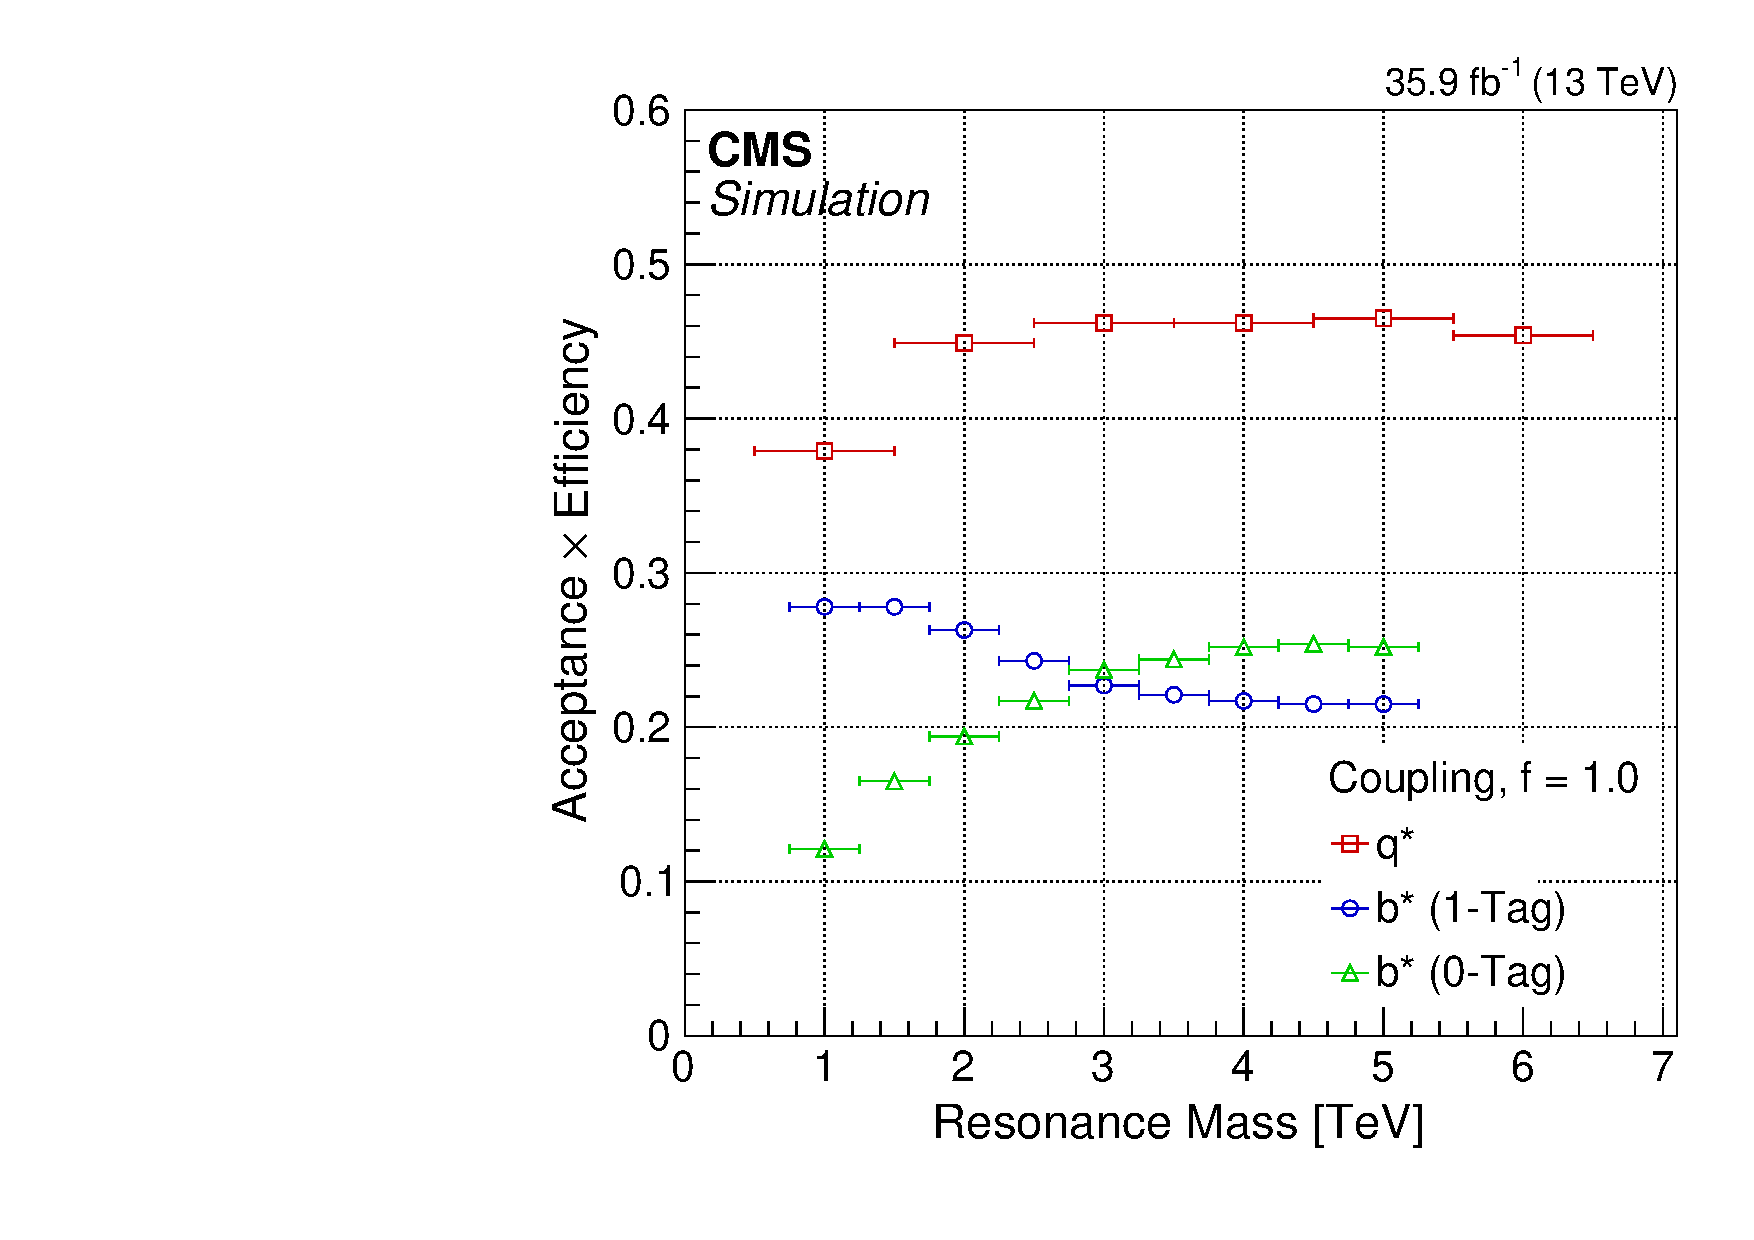
\includegraphics[width=9.5cm]{Chapter4/Acc_times_eff/AccXEff.pdf}
\caption{The product of acceptance and efficiency as a function of \qstar and \bstar mass for SM coupling, $f$ $=$ 1.0, obtained using MC simulation.}
\label{fig:accEff}
\end{figure}
\vspace{-0.1in}

{\color{white}.}

A comparison between Data and MC for different kinematical variables for photons and jets,
after final selection, corresponding to the three categories viz. no b-tag, 1 b-tag and
0 b-tag, are presented in \fig{\ref{fig:PtDist}}, \fig{\ref{fig:EtaDist}} and \fig{\ref{fig:PhiDist}} respectively. These distributions are found to be in
reasonable agreement with the theoretical predictions. The \pt\ distribution for data falls steeply with the increasing \pt and agrees well with MC within the
uncertainties. Likewise, the $\eta$ distribution is in good agreement with the shape anticipated by MC. 

The distributions of photons and jets in $\Delta\eta$, $\Delta\phi$ and ${\Delta}$R are also presented in \fig{\ref{fig:deta}}. The number of photons,
jets and b-jets per event are shown in \fig{\ref{fig:mult}}. The Data-MC comparison of the invariant mass distributions of $\gamjet$ and $\gambjet$
in three categories is displayed in \fig{\ref{fig:InvtMass_DataMC}}.

The various kinematical distributions depicted here confirm that the kinematics of analysis objects in detector data comply with the theoretical expectations.
However, the theoretical MC simulations, in this analysis, are used just to check the behaviour of the data. The actual backgrounds for the processes under study,
have been computed using a data driven technique by fitting the invariant mass distribution spectra with a smooth parameterization.

\begin{figure}[htbp]
\centering
\subfloat[$\pt^{\gamma}$]{\label{fig:Ph_pt}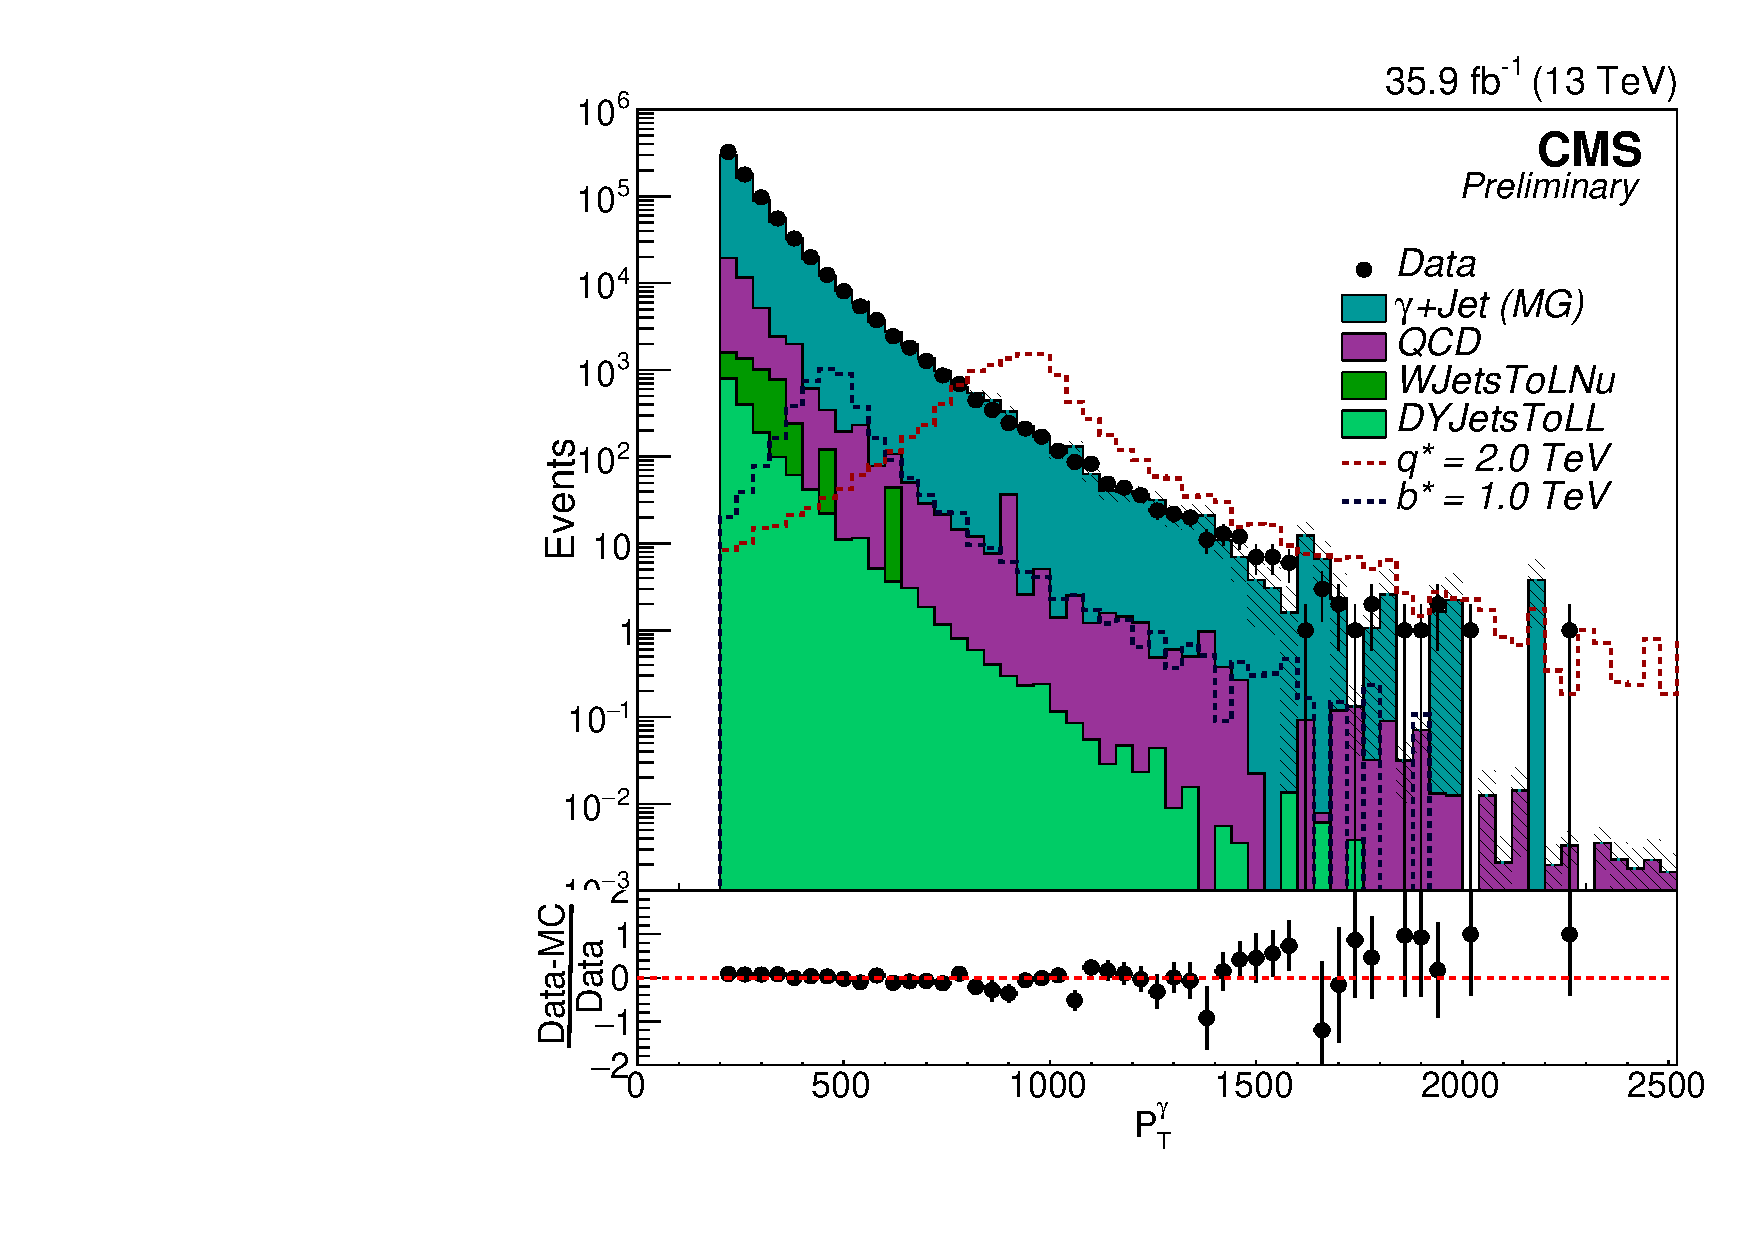
\includegraphics[width=6.8cm]{Chapter4/Kinematics/PhPt_Notag.pdf}} \hspace{0.2in}
\subfloat[$\pt^{\textrm{jet}}$]{\label{fig:Jet_pt}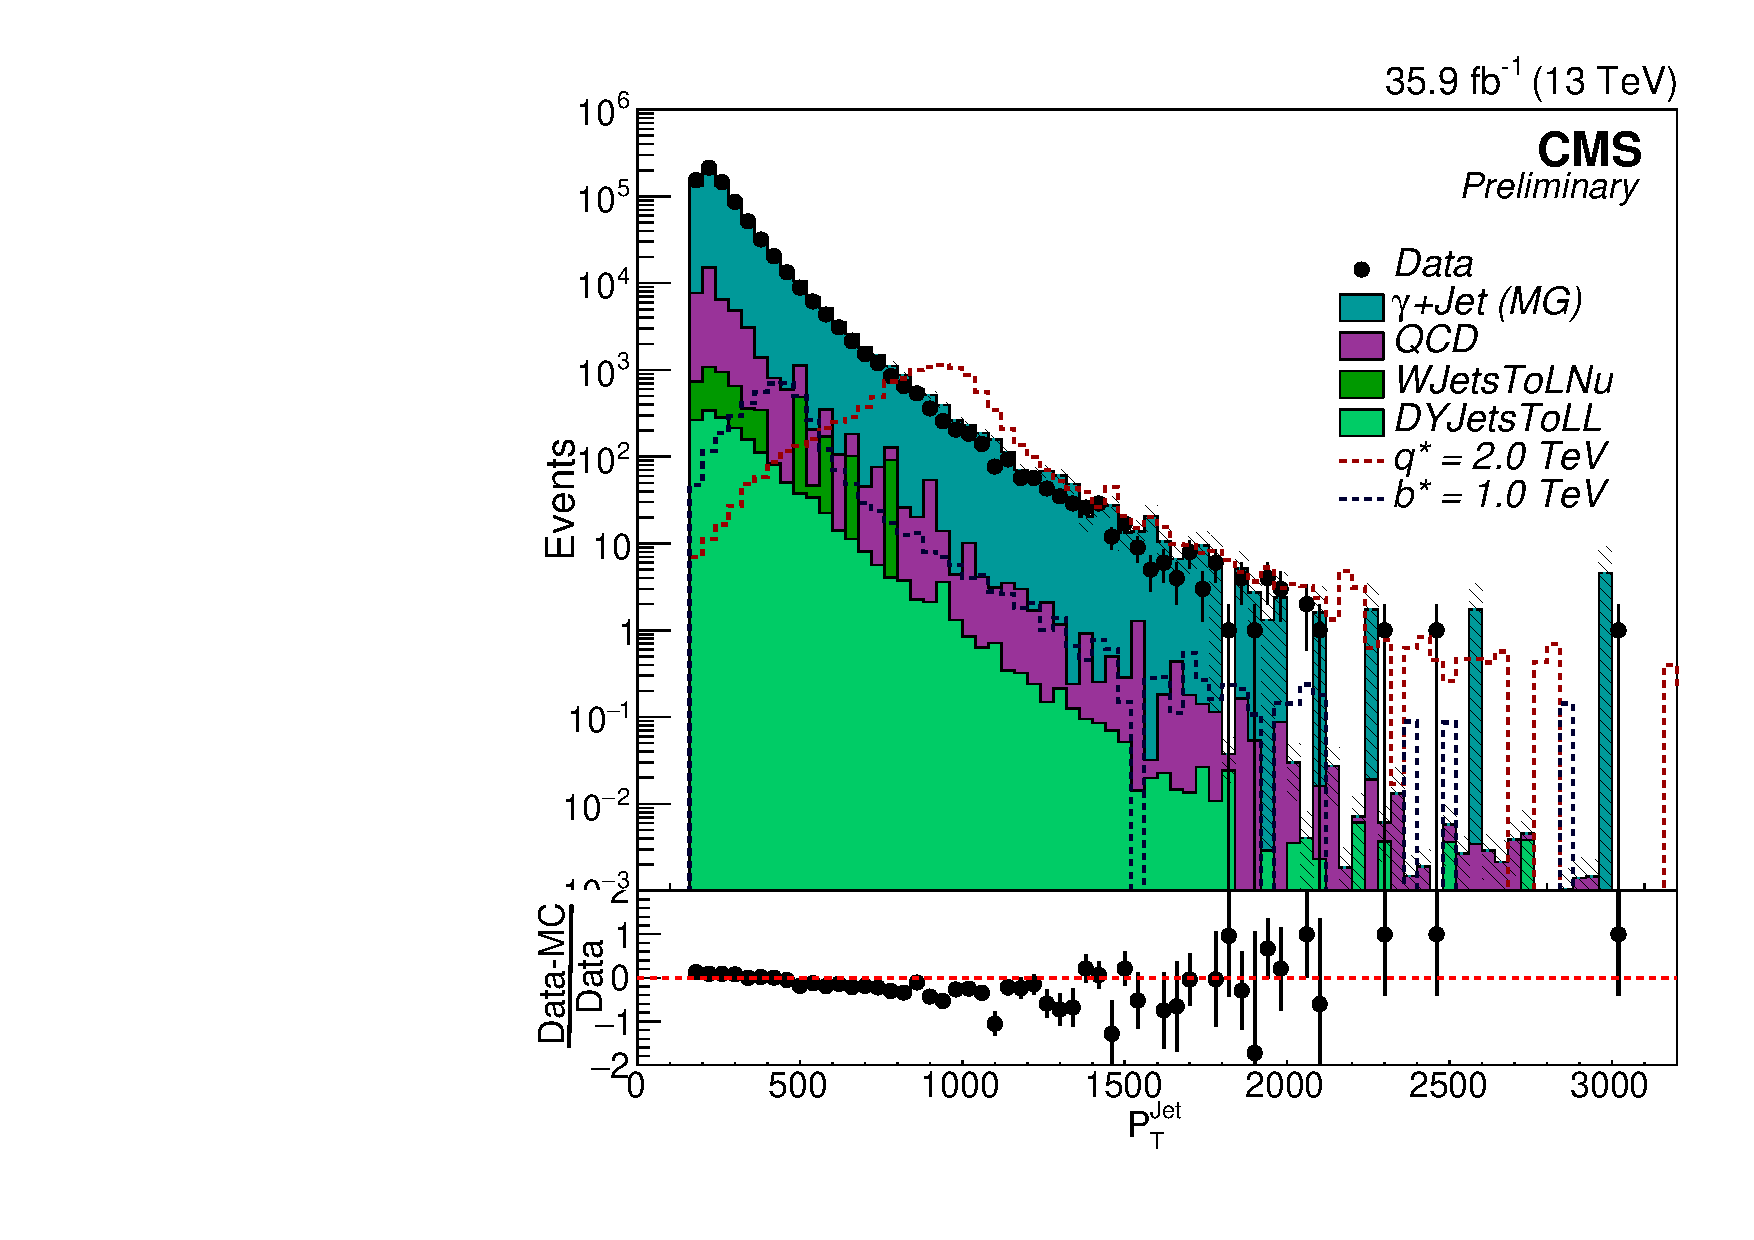
\includegraphics[width=6.8cm]{Chapter4/Kinematics/JetPt_Notag.pdf}}\\
\subfloat[$\pt^{\gamma}(1 \textrm{ b-tag})$]{\label{fig:Ph_pt_1tag}\includegraphics[width=6.8cm]{Chapter4/Kinematics/PhPt_1tag.pdf}} \hspace{0.2in}
\subfloat[$\pt^{\textrm{jet}}(1 \textrm{ b-tag})$]{\label{fig:1bJet_pt}\includegraphics[width=6.8cm]{Chapter4/Kinematics/JetPt_1tag.pdf}}\\
\subfloat[$\pt^{\gamma}(0 \textrm{ b-tag})$]{\label{fig:Ph_pt_0tag}\includegraphics[width=6.8cm]{Chapter4/Kinematics/PhPt_0tag.pdf}} \hspace{0.2in}
\subfloat[$\pt^{\textrm{jet}}(0 \textrm{ b-tag})$]{\label{fig:0bJet_pt}\includegraphics[width=6.8cm]{Chapter4/Kinematics/JetPt_0tag.pdf}}
\caption{Data-MC comparison of \pt distribution of photons and jets for three categories: no b-tag, 1 b-tag and 0 b-tag.}
\label{fig:PtDist}
\end{figure}


\begin{figure}[htbp]
\centering
\subfloat[${\eta}^{\gamma}$]{\label{fig:Ph_eta}\includegraphics[width=6.8cm]{Chapter4/Kinematics/PhEta_Notag.pdf}} \hspace{0.2in}
\subfloat[${\eta}^{\textrm{jet}}$]{\label{fig:Jet_eta}\includegraphics[width=6.8cm]{Chapter4/Kinematics/JetEta_Notag.pdf}}\\
\subfloat[${\eta}^{\gamma}(1 \textrm{ b-tag})$]{\label{fig:Ph_eta_1tag}\includegraphics[width=6.8cm]{Chapter4/Kinematics/PhEta_1tag.pdf}} \hspace{0.2in}
\subfloat[${\eta}^{\textrm{jet}}(1 \textrm{ b-tag})$]{\label{fig:1bJet_eta}\includegraphics[width=6.8cm]{Chapter4/Kinematics/JetEta_1tag.pdf}}\\
\subfloat[${\eta}^{\gamma}(0 \textrm{ b-tag})$]{\label{fig:Ph_eta_0tag}\includegraphics[width=6.8cm]{Chapter4/Kinematics/PhEta_0tag.pdf}} \hspace{0.2in}
\subfloat[${\eta}^{\textrm{jet}}(0 \textrm{ b-tag})$]{\label{fig:0bJet_eta}\includegraphics[width=6.8cm]{Chapter4/Kinematics/JetEta_0tag.pdf}}
\caption{Data-MC comparison of $\eta$ distribution of photons and jets for three categories: no b-tag, 1 b-tag and 0 b-tag.}
\label{fig:EtaDist}
\end{figure}

\begin{figure}[htbp]
\centering
\subfloat[${\phi}^{\gamma}$]{\label{fig:Ph_phi}\includegraphics[width=6.8cm]{Chapter4/Kinematics/PhPhi_Notag.pdf}} \hspace{0.2in}
\subfloat[${\phi}^{\textrm{jet}}$]{\label{fig:Jet_phi}\includegraphics[width=6.8cm]{Chapter4/Kinematics/JetPhi_Notag.pdf}}\\
\subfloat[${\phi}^{\gamma}(1 \textrm{ b-tag})$]{\label{fig:Ph_phi_1tag}\includegraphics[width=6.8cm]{Chapter4/Kinematics/PhPhi_1tag.pdf}} \hspace{0.2in}
\subfloat[${\phi}^{\textrm{jet}}(1 \textrm{ b-tag})$]{\label{fig:1bJet_phi}\includegraphics[width=6.8cm]{Chapter4/Kinematics/JetPhi_1tag.pdf}}\\
\subfloat[${\phi}^{\gamma}(0 \textrm{ b-tag})$]{\label{fig:Ph_phi_0tag}\includegraphics[width=6.8cm]{Chapter4/Kinematics/PhPhi_0tag.pdf}} \hspace{0.2in}
\subfloat[${\phi}^{\textrm{jet}}(0 \textrm{ b-tag})$]{\label{fig:0bJet_phi}\includegraphics[width=6.8cm]{Chapter4/Kinematics/JetPhi_0tag.pdf}}
\caption{Data-MC comparison of ${\phi}$ distribution of photons and jets for three categories: no b-tag, 1 b-tag and 0 b-tag.}
\label{fig:PhiDist}
\end{figure}



\begin{figure}[htbp]
\centering
\includegraphics[width=5.3cm]{Chapter4/PhJetDist/DEta_GJet.pdf} \hspace{0.2in}
\includegraphics[width=5.3cm]{Chapter4/PhJetDist/DPhi_GJet.pdf}
\includegraphics[width=5.3cm]{Chapter4/PhJetDist/DR_GJet.pdf}
\caption{Distributions of photons and jets in $\Delta\eta$ (above left), $\Delta\phi$ (above right), and $\Delta$R (below).}
\label{fig:deta}
\end{figure}
\vspace{-0.3in}
\begin{figure}[htbp]
\centering
\includegraphics[width=5.3cm]{Chapter4/Multiplicity/nIsoph.pdf} \hspace{0.2in}
\includegraphics[width=5.3cm]{Chapter4/Multiplicity/njets.pdf}
\includegraphics[width=5.3cm]{Chapter4/Multiplicity/nbjets.pdf}
\caption{Number of photons (above left), jets (above right), and b-jets (below) per event in Data-MC.}
\label{fig:mult}
\end{figure}


\begin{figure}[htbp]
\centering
\subfloat[M$_{\gamjet}$]{\label{fig:InvtMass_q}\includegraphics[width=10.0cm]{Chapter4/PhJetDist/InvtMass_GJet.pdf}}\\ \vspace{0.4in}
\subfloat[M$_{\gamjet}$(1 b-tag)]{\label{fig:InvtMass_b}\includegraphics[width=8.0cm]{Chapter4/PhJetDist/InvtMass_GbJet.pdf}}
\subfloat[M$_{\gamjet}$(0 b-tag)]{\label{fig:InvtMass_b0}\includegraphics[width=8.0cm]{Chapter4/PhJetDist/InvtMass_GbJet_0tag.pdf}}
\caption{Data-MC comparison of invariant mass distribution of $\gamjet$ in three categories: no b-tag, 1 b-tag and 0 b-tag.}
\label{fig:InvtMass_DataMC}
\end{figure}


\subsection{Optimization of event selection}
The event selection considered in this analysis has been optimized for best expected mass limits on \qstar and \bstar resonances
(the procedure to obtain expected limits is explained in the upcoming
\sectn{\ref{Se:Limits}}). The expected background obtained from the Poisson fluctuation of total background MC has been used in evaluating limits. The
standard selection used for optimization study is ``loose'' photon ID, ``tight'' jet ID, $\Delta\eta$ $<$ 1.8, $\Delta\phi$ $>$ 1.5 and ``medium'' CSVv2 cut.

For different photon ID working points (WP), the expected limits at 95$\%$ CL are presented in \fig{\ref{fig:PhIDOpti}} and \tab{\ref{Table:PhIDOpti}}. 
The optimization study tells that the ``loose'' WP is the most efficient one. However, it has been found that the trigger efficiency w.r.t muon reference trigger
improves on going from loose to medium WP, therefore, ``medium'' WP for photon ID has been chosen. 

\vspace{-0.1in}
%%Photon ID
\begin{table}[htbp]
  \begin{minipage}{0.54\textwidth}
    \begin{figure}[H]
      \includegraphics[width=8.2cm]{Chapter4/Optimization/Explimits_Optimization_freq_PhId_Opti_Qstar_excitedquarks2016.pdf}
      \caption{Expected 95$\%$ CL upper limits on $\sigma$ $\times$ BR $\times$ A $\times$ $\epsilon$ versus \qstar mass
        for different photon ID cuts corresponding to SM coupling $f$ $=$ 1.0.}
      \label{fig:PhIDOpti}
    \end{figure}
  \end{minipage}%
  \hfill
  \begin{minipage}{0.44\textwidth}
    \centering
    \resizebox{6.0cm}{!}{
      \begin{tabular}{lc}
        \toprule
        \belowrulesepcolor{Mygray}
        \belowrulesepcolor{Mygray}
        \belowrulesepcolor{Mygray}
        \rowcolor{Mygray}[\dimexpr\tabcolsep+0.09pt\relax]
        \bf {Photon ID}    &  \bf {Exp. mass } \\
        \belowrulesepcolor{Mygray}
        \rowcolor{Mygray}[\dimexpr\tabcolsep+0.09pt\relax]
                           &  \bf {limit (TeV)} \\
        \aboverulesepcolor{Mygray}
        \aboverulesepcolor{Mygray}
        \aboverulesepcolor{Mygray}
        \midrule
        \bf {loose}   &  5.17  \\
        \bf {medium}  &  5.11  \\
        \bf {tight}   &  5.13  \\
        \bottomrule
      \end{tabular}
    }
    \caption{Photon ID cut optimization corresponding to different mass expected limits.}
    \label{Table:PhIDOpti}
  \end{minipage}
\end{table}
\vspace{-0.1in}

The optimization studies for different $\Delta\eta$ cuts is presented in \fig{\ref{fig:DEtaOpti}} and \tab{\ref{Table:DEtaOpti}} and
a $\Delta\eta$($\gamma$, jet) cut of 1.5 is found to be the most efficient. One more advantage of a $\Delta\eta$($\gamma$, jet)
cut is that it helps in achieving mass turn-on at a lower mass point (as shown in \fig{\ref{fig:MassTurnOn}}) compared to no $\Delta\eta$ cut.  

The corresponding optimization results for various $\Delta\phi$ cuts are presented in \fig{\ref{fig:DPhiOpti}} and \tab{\ref{Table:DPhiOpti}} while for various CSVv2
cuts, it is presented in \fig{\ref{fig:BTagOpti}} and \tab{\ref{Table:BTagOpti}}. A selection without any $\Delta\phi$ cut and a ``loose'' CSVv2 cut is found optimum.

\vspace{-0.1in}
%% DEta 
\begin{table}[htbp]
  \begin{minipage}{0.54\textwidth}
    \begin{figure}[H]
      \includegraphics[width=8.2cm]{Chapter4/Optimization/Explimits_Optimization_freq_DEta_Opti_Qstar_excitedquarks2016.pdf}
      \caption{Expected 95$\%$ CL upper limits on $\sigma$ $\times$ BR $\times$ A $\times$ $\epsilon$ versus \qstar mass
        for different ${\Delta}{\eta}$ cuts corresponding to SM coupling $f$ $=$ 1.0.}
      \label{fig:DEtaOpti}
    \end{figure}
  \end{minipage}%
  \hfill
  \begin{minipage}{0.44\textwidth}
    \centering
    \resizebox{6cm}{!}{
      \begin{tabular}{lc}
        \toprule
        \belowrulesepcolor{Mygray}
        \belowrulesepcolor{Mygray}
        \belowrulesepcolor{Mygray}
        \rowcolor{Mygray}[\dimexpr\tabcolsep+0.09pt\relax]
        \bf {${\Delta}{\eta}$ cuts}    &  \bf {Exp. mass} \\
        \belowrulesepcolor{Mygray}
        \rowcolor{Mygray}[\dimexpr\tabcolsep+0.09pt\relax]
                                       &  \bf {limit (TeV)} \\
        \aboverulesepcolor{Mygray}
        \aboverulesepcolor{Mygray}
        \aboverulesepcolor{Mygray}
        \midrule
        \bf {${\Delta}{\eta}$ $<$ 1.0}  &  5.17    \\
        \bf {${\Delta}{\eta}$ $<$ 1.2}  &  5.31    \\
        \bf {${\Delta}{\eta}$ $<$ 1.5}  &  5.39    \\
        \bf {${\Delta}{\eta}$ $<$ 1.8}  &  5.27     \\ 
        \bf {${\Delta}{\eta}$ $<$ 2.0}  &  5.28     \\
        \bf {${\Delta}{\eta}$ $<$ 2.2}  &  5.24     \\
        \bf {${\Delta}{\eta}$ $<$ 2.5}  &  5.19     \\
        \bf {No ${\Delta}{\eta}$}      &  5.26       \\
        \bottomrule
      \end{tabular}
    }
    \caption{${\Delta}{\eta}$ cut optimization corresponding to different mass expected limits.}
    \label{Table:DEtaOpti}
  \end{minipage}
\end{table}
\vspace{-0.1in}

%%%%%%%%%%%%%%%%%%%%%%%%%%%%%%%%%%%%%%%%%%%%%%%%%%%%%%%%%%%%%%%%%%%%%%%%%%%%%%%%%%%%%%%%%%%%%%%%%%%%%%%%%%%%%%%%%%%%%%%%%%%%%%%%%%%%%%%%%%%
%% %% Jet ID                                                                                                                             %%
%% \begin{table}[htbp]                                                                                                                   %%
%%   \begin{minipage}{0.55\textwidth}                                                                                                    %%
%%     \begin{figure}[H]                                                                                                                 %%
%%       \includegraphics[width=8.5cm]{Chapter4/Optimization/Explimits_Optimization_freq_JetId_Opti_Qstar_excitedquarks2016.pdf}         %%
%%       \caption{The expected 95$\%$ CL upper limits on $\sigma$ $\times$ BR $\times$ A $\times$ $\epsilon$ for excited quarks compared %%
%%         with theory predictions for different jet ID cuts corresponding to SM coupling $f$ $=$ 1.0.}                                  %%
%%       \label{fig:JetIDOpti}                                                                                                           %%
%%     \end{figure}                                                                                                                      %%
%%   \end{minipage}%                                                                                                                     %%
%%   \hfill                                                                                                                              %%
%%   \begin{minipage}{0.45\textwidth}                                                                                                    %%
%%     \centering                                                                                                                        %%
%%     \resizebox{7cm}{!}{                                                                                                               %%
%%       \begin{tabular}{lc}                                                                                                             %%
%%         \toprule                                                                                                                      %%
%%         \belowrulesepcolor{Mygray}                                                                                                    %%
%%         \belowrulesepcolor{Mygray}                                                                                                    %%
%%         \belowrulesepcolor{Mygray}                                                                                                    %%
%%         \rowcolor{Mygray}[\dimexpr\tabcolsep+0.09pt\relax]                                                                            %%
%%         \bf {Jet ID}    &  \bf {Exp. mass limit (TeV)} \\                                                                             %%
%%         \aboverulesepcolor{Mygray}                                                                                                    %%
%%         \aboverulesepcolor{Mygray}                                                                                                    %%
%%         \aboverulesepcolor{Mygray}                                                                                                    %%
%%         \midrule                                                                                                                      %%
%%         \bf {tight}   &  5.24  \\                                                                                                     %%
%%         \bf {tightLepVeto}  &  5.05  \\                                                                                               %%
%%         \bottomrule                                                                                                                   %%
%%       \end{tabular}                                                                                                                   %%
%%     }                                                                                                                                 %%
%%     \caption{Jet ID cut optimization corresponding to different mass expected limits.}                                                %%
%%     \label{Table:JetIDOpti}                                                                                                           %%
%%   \end{minipage}                                                                                                                      %%
%% \end{table}                                                                                                                           %%
%%%%%%%%%%%%%%%%%%%%%%%%%%%%%%%%%%%%%%%%%%%%%%%%%%%%%%%%%%%%%%%%%%%%%%%%%%%%%%%%%%%%%%%%%%%%%%%%%%%%%%%%%%%%%%%%%%%%%%%%%%%%%%%%%%%%%%%%%%%



%\begin{figure}[h]
%\centering
%\subfloat[No ${\Delta}{\eta}$ cut]{\label{fig:deta_no}\includegraphics[width=6.5cm]{Chapter4/MassTurnOn/MassTurnOn_noDeta.pdf}}
%\hspace{0.2 in}
%\subfloat[With ${\Delta}{\eta}$ cut]{\label{fig:deta_yes}\includegraphics[width=6.5cm]{Chapter4/MassTurnOn/MassTurnOn_afterfinalselection.pdf}}
%\caption{Impact of ${\Delta}{\eta}$ cut on mass turn-on.}
%\label{fig:deta_gof}
%\end{figure}

%% DPhi
\begin{table}[htbp]
  \begin{minipage}{0.54\textwidth}
    \begin{figure}[H]
      \includegraphics[width=8.2cm]{Chapter4/Optimization/Explimits_Optimization_freq_DPhi_Opti_Qstar_excitedquarks2016.pdf}
      \caption{Expected 95$\%$ CL upper limits on $\sigma$ $\times$ BR $\times$ A $\times$ $\epsilon$ versus \qstar mass
        for different ${\Delta}{\phi}$ cuts corresponding to SM coupling $f$ $=$ 1.0.}
      \label{fig:DPhiOpti}
    \end{figure}
  \end{minipage}%
  \hfill
  \begin{minipage}{0.44\textwidth}
    \centering
    \resizebox{6cm}{!}{
      \begin{tabular}{lc}
        \toprule
        \belowrulesepcolor{Mygray}
        \belowrulesepcolor{Mygray}
        \belowrulesepcolor{Mygray}
        \rowcolor{Mygray}[\dimexpr\tabcolsep+0.09pt\relax]
        \bf {${\Delta}{\phi}$ cuts}    &  \bf {Exp. mass} \\
        \belowrulesepcolor{Mygray}
        \rowcolor{Mygray}[\dimexpr\tabcolsep+0.09pt\relax]
                                       &  \bf {limit (TeV)} \\
        \aboverulesepcolor{Mygray}
        \aboverulesepcolor{Mygray}
        \aboverulesepcolor{Mygray}
        \midrule
        \bf {${\Delta}{\phi}$ $>$ 1.5}  &  5.19   \\
        \bf {${\Delta}{\phi}$ $>$ 2.0}  &  5.17    \\
        \bf {${\Delta}{\phi}$ $>$ 2.5}  &  5.18     \\
        \bf {No ${\Delta}{\phi}$}       &  5.24     \\
        \bottomrule
      \end{tabular}
    }
    \caption{${\Delta}{\phi}$ cut optimization corresponding to different mass expected limits.}
    \label{Table:DPhiOpti}
  \end{minipage}
\end{table}

%% CSVv2
\begin{table}[htbp]
  \begin{minipage}{0.54\textwidth}
    \begin{figure}[H]
      \includegraphics[width=8.2cm]{Chapter4/Optimization/Explimits_Optimization_freq_CSVDisc_Opti_Bstar_excited1btagquarks2016.pdf}
      \caption{Expected 95$\%$ CL upper limits on $\sigma$ $\times$ BR $\times$ A $\times$ $\epsilon$ versus \qstar mass
        for different CSVv2 cuts corresponding to SM coupling $f$ $=$ 1.0.}
      \label{fig:BTagOpti}
    \end{figure}
  \end{minipage}%
  \hfill
  \begin{minipage}{0.44\textwidth}
    \centering
    \resizebox{7cm}{!}{
      \begin{tabular}{lc}
        \toprule
        \belowrulesepcolor{Mygray}
        \belowrulesepcolor{Mygray}
        \belowrulesepcolor{Mygray}
        \rowcolor{Mygray}[\dimexpr\tabcolsep+0.09pt\relax]
        \bf {CSVv2}    &  \bf {Exp. mass} \\
        \belowrulesepcolor{Mygray}
        \rowcolor{Mygray}[\dimexpr\tabcolsep+0.09pt\relax]
                       &  \bf {limit (TeV)} \\
        \aboverulesepcolor{Mygray}
        \aboverulesepcolor{Mygray}
        \aboverulesepcolor{Mygray}
        \midrule
        \bf {loose}   &  1.73  \\
        \bf {medium}  &  1.70  \\
        \bf {tight}   &  1.50  \\
        \bottomrule
      \end{tabular}
    }
    \caption{CSVv2 cut optimization corresponding to different mass expected limits.}
    \label{Table:BTagOpti}
  \end{minipage}
\end{table}
%\vspace{-0.15in}
\section{Highest invariant mass events in data}
The event with highest invariant mass is observed in data at M$_{\gamjet}$ $=$ 4616.69\unit{GeV}. The event display for this event has been made using
the cmsShow~\cite{Web:cmsShow} package in different detector orientations and is presented in \fig{\ref{fig:evtDisplay_highest}}. The photon candidate
in this event is found to have a \pt $=$ 1253\unit{GeV} and $\eta$ $=$ $-$0.857733 while the jet candidate has a \pt $=$ 3022.47\unit{GeV} and
$\eta$ $=$ 0.395303. The jet candidate is tagged as a b-jet, therefore, this event form the highest \qstar as well as the highest \bstar
invariant mass event. This event was recorded by the CMS detector on 29$^{\textrm{th}}$ August, 2016 in the run number 279716.

The event with 2$^{\textrm{nd}}$ highest invariant mass is observed at M$_{\gamjet}$ $=$ 4595.43\unit{GeV} with the photon candidate having \pt $=$ 1872.51\unit{GeV},
$\eta$ $=$ 0.927873 and the jet candidate having \pt $=$ 1945.66\unit{GeV}, $\eta$ $=$ $-$0.299033. Since the jet is not tagged as a b-jet, so this event form
the part of \qstar\ statistics only. The event display for this event is presented in \fig{\ref{fig:evtDisplay_2ndhighest}}. 

\clearpage
\begin{figure}[]
\centering
\subfloat[$\rho$-$\phi$ plane]{\label{fig:rhophi}\includegraphics[width=8.5cm]{Chapter4/EventDisplay/ED-M4616_279716-1104-1960082201_RhoPhi_InvtMass-4616.pdf}} 
\subfloat[3-dimensional plane]{\label{fig:3d}\includegraphics[width=8.5cm]{Chapter4/EventDisplay/ED-M4616_279716-1104-1960082201_3D_InvtMass-4616.pdf}}
\caption{Event display for the highest invariant mass event at M$_{\gamjet}$ $=$ 4616.69\unit{GeV}. This event has the jet tagged as a b-jet, thereby, forming
  a highest \qstar as well as highest \bstar event.}
\label{fig:evtDisplay_highest}
\end{figure}

\begin{figure}[]
\centering
\subfloat[$\rho$-$\phi$ plane]{\label{fig:2nd_rhophi}\includegraphics[width=8.5cm]{Chapter4/EventDisplay/ED-M4595_276811-166-275256142_RhoPhi_InvtMass-4595.pdf}} 
\subfloat[3-dimensional plane]{\label{fig:2nd_3d}\includegraphics[width=8.5cm]{Chapter4/EventDisplay/ED-M4595_276811-166-275256142_3D_InvtMass4595.pdf}}
\caption{Event display for the 2$^{\textrm{nd}}$ highest invariant mass event at M$_{\gamjet}$ $=$ 4595.43\unit{GeV}.}
\label{fig:evtDisplay_2ndhighest}
\end{figure}
\clearpage

\section{Signal spectrum}
The $\gamjet/$b-jet invariant mass distribution spectrum falls steeply with increasing mass. The \qstar and \bstar signals, if exist, will appear
as narrow resonances over the continuous spectrum. In order to observe these narrow resonances, the bin widths of invariant mass distributions should
match with the mass resolutions of the \qstar and \bstar resonances. Since the resonance width and hence the mass resolution is directly proportional to the
resonance mass, it increases with increase of resonance mass. So the invariant mass spectra are required to have a variable binning with increasing bin widths.

To obtain variable binning, the signal shape at different masses are fitted with three different functions, viz.\ Gaussian, Breit-Wigner and Crystal-Ball (CB), as
shown in \fig{\ref{fig:SigFitting}} for some of \qstar mass points. This is required to retrieve the mass resolutions. The Crystal-Ball
function is found to best describe the shapes and its functional form is given by,

\vspace{-0.3in}
\begin{equation}
CB(x; \alpha, n, \mu, \sigma) = N_{CB} \cdot \left\lbrace \begin{array}{lr}
\exp\left( -\frac{(x-\mu)^2}{2\sigma^2}\right) , & \quad \text{for } \frac{x-\mu}{\sigma} > -\alpha \\
{\left( \frac{n}{|\alpha |}\right)}^n \cdot \exp \left(-\frac{|\alpha|^2}{2}\right) \cdot \left(\frac{n}{|\alpha|}-|\alpha| - \frac{x-\mu}{\sigma}\right)^{-n} , & \quad \text{for } \frac{x-\mu}{\sigma} \leq -\alpha ,
\end{array}
\right.
\label{eq:crystalball}
\end{equation}
where $N_{CB}$ is the normalization factor, $\sigma$ is the width, $\mu$ is the mean and $\alpha, n$ are the parameters determining the functional fitting.
The resonance widths and means obtained from CB fitting are then used in a functional form,
\begin{equation}
  \frac{\sigma}{\textrm{Mean}} = \textrm{A} + \frac{\textrm{B}}{\textrm{M}_{\textrm{Res}}}
\end{equation}
where $\frac{\sigma}{\textrm{Mean}}$ is known as the mass resolution with $\sigma$, the resonance width and Mean, the resonance mean obtained upon fitting
and M$_{\textrm{Res}}$ is the resonance mass. This functional form is plotted between $\frac{\sigma}{\textrm{Mean}}$ and M$_{\textrm{Res}}$ for different masses
and fitted to obtain the values of parameters A and B as shown in \fig{\ref{fig:MassResolution}}. These parameters are then used to obtain variable mass binning
for \qstar and \bstar invariant mass distributions and is presented below:

\vspace{-0.1in}
\scriptsize
\begin{verbatim}
nMassBin[120] = { 1, 3, 6, 10, 16, 23, 31, 40, 50, 61, 73, 86, 100, 115, 132, 150, 169, 
                  189, 210, 232, 252, 273, 295, 318, 341, 365, 390, 416, 443, 471, 500, 
                  530, 561, 593, 626, 660, 700, 731, 768, 806, 846, 887, 929, 972, 1017,
                  1063, 1110, 1159, 1209, 1261, 1315, 1370, 1427, 1486, 1547, 1609, 1673, 
                  1739, 1807, 1877, 1950, 2025, 2102, 2182, 2264, 2349, 2436, 2526, 2619,
                  2714, 2812, 2913, 3018, 3126, 3237, 3352, 3470, 3592, 3718, 3847, 3980,
                  4117, 4259, 4405, 4556, 4711, 4871, 5036, 5206, 5381, 5562, 5748, 5940,
                  6138, 6342, 6552, 6769, 6993, 7223, 7461, 7706, 7959, 8219, 8487, 8764, 
                  9049, 9343, 9646, 9958, 10280, 10612, 10954, 11307, 11671, 12046, 12432,
                  12830, 13241, 13664, 14000};
\end{verbatim}
\normalsize

\vspace{-0.1in}
\begin{figure}[htbp]
\centering
\subfloat[M$_{\qstar}$ $=$ 1000\unit{GeV}]{\label{fig:q_1000}\includegraphics[width=5.4cm]{Chapter4/SignalFitting/Qstar1000.pdf}} 
\subfloat[M$_{\qstar}$ $=$ 2000\unit{GeV}]{\label{fig:q_2000}\includegraphics[width=5.4cm]{Chapter4/SignalFitting/Qstar2000_bin25.pdf}} 
\subfloat[M$_{\qstar}$ $=$ 3000\unit{GeV}]{\label{fig:q_3000}\includegraphics[width=5.4cm]{Chapter4/SignalFitting/Qstar3000_bin25.pdf}}
\caption{Fitting the core of invariant mass of \qstar signal at different masses for $f$ $=$ 1.0, using Breit-Wigner (Blue), Crystal-Ball (Red), and Gaussian
(Green) functions to obtain the resonance width of the signal.}
\label{fig:SigFitting}
\end{figure}

\vspace{-0.1in}
\begin{figure}[h!]
\centering
\includegraphics[width=8.5cm,height=5.95cm]{Chapter4/SignalFitting/Fit_SigmaMean_v1.pdf}
 \caption{Polynomial fitting of mass resolution vs.\ resonance mass to obtain variable binning parameters.}
 \label{fig:MassResolution}
\end{figure}
\vspace{-0.1in}

\section{Signal interpolation}
While searching for new particles, with unknown masses, it is essential to scan the entire possible mass range. Due to limitation of resources, only a
limited number of signal masses over a large range are generated. For \qstar (\bstar) resonances, only 10 mass points per coupling multiplier are generated
in the mass range from 0.5$-$9.0\unit{TeV} (0.5$-$5.0\unit{TeV}). The signal shapes at intermediate masses are obtained by using an interpolation
technique~\cite{Interpolation} which utilizes the information from neighbouring generated masses. 

In order to interpolate a signal shape at an intermediate mass M between two generated masses M$_{\textrm{A}}$ and M$_{\textrm{B}}$ using this
technique, a probability distribution
in a parameter X is constructed which is defined as Prob.(X) = $\frac{\textrm{M}_{\gamjet}}{\textrm{M}_{\textrm{Res}}}$, where M$_{\textrm{Res}}$ is the resonance
mass and M$_{\gamjet}$ is the invariant mass distribution at the resonance mass. This distribution for masses M$_{\textrm{A}}$ and M$_{\textrm{B}}$
are obtained and used to get the Prob.(X) distribution for mass M using the relation,
\begin{equation}
  \textrm{Prob}_{\textrm{M}}(\textrm{X}) = \textrm{Prob}_{\textrm{M}_{\textrm{A}}}(\textrm{X}) + [ \textrm{Prob}_{\textrm{M}_{\textrm{B}}}(\textrm{X}) - \textrm{Prob}_{\textrm{M}_{\textrm{A}}}(\textrm{X}) ]
  \cdot \frac{\textrm{M} - \textrm{M}_{\textrm{A}}}{\textrm{M}_{\textrm{B}} - \textrm{M}_{\textrm{A}}}
\end{equation}

The X$-$distribution is then converted back to $\gamjet$ mass distribution using the ROOT::Math::Interpolator~\cite{Brun:1997pa} class
to get the resonance shape at the interpolated resonance mass. The generated and interpolated signal shapes for different \qstar\ mass points
are plotted alternatively for comparison in the \fig{\ref{fig:ResShapes}}. 

\begin{figure}[h]
\centering
\includegraphics[width=12cm]{Chapter4/Interpolation/Gen_n_Int_shapes.pdf}
\caption{Alternate generated (solid line) and interpolated (dotted line) shapes for different \qstar mass points.}
\label{fig:ResShapes}
\end{figure}

\begin{figure}[h]
\centering
\subfloat[\qstar $=$ 2.0\unit{TeV}]{\label{}\includegraphics[width=5.2cm]{Chapter4/Interpolation/Int_vs_gen_qstar2Tev.pdf}}
\subfloat[\qstar $=$ 4.0\unit{TeV}]{\label{}\includegraphics[width=5.2cm]{Chapter4/Interpolation/Int_vs_gen_qstar4Tev.pdf}}
\subfloat[\qstar $=$ 6.0\unit{TeV}]{\label{}\includegraphics[width=5.2cm]{Chapter4/Interpolation/Int_vs_gen_qstar6Tev.pdf}}
\caption{Comparison of generated and interpolated shapes at different \qstar mass points.}
\label{fig:ShapeComp}
\end{figure}

The interpolation procedure has been authenticated by performing a closure test in which already generated shapes from \pythia are interpolated again using
the immediate neighbours and a comparison is made as shown in \fig{\ref{fig:ShapeComp}} for three different \qstar mass points.
The interpolated shapes are found to be in good agreement with the generated ones. Only a small difference is observed on going towards higher masses, which is
considered as a systematic uncertainty.

\section{Parametric background}
The invariant mass distributions of $\gamjet$ and $\gambjet$ are well described by MC simulation. The binning of invariant mass
distribution is chosen to have a bin width almost equal to the expected \qstar and \bstar mass resolutions, that varies from about 4.5$\%$ at
1\unit{TeV} to 3.3$\%$ at 6\unit{TeV}. However, in order to model the background of this study, a data driven method using a smooth parameterization
has been considered. The usage of a fit function is advantageous over MC simulation in background modelling as MC simulation has many theoretical
(like PDFs, renormalization scale etc.) and experimental (like jet energy scale, energy resolutions etc.) uncertainties associated with it. 
The methodology of smooth parameterization is considered because the background due to $\gamjet$ processes is smooth and monotonically falling
and can be extracted by fitting the distribution with a smooth polynomial function. 

Several functional forms inspired from previous similar searches~\cite{Aaltonen:2008dn, Harris:2011bh, ATLAS:2011ai, Chatrchyan:2013qha, Aad:2013cva, CMS_qstartogammaJet_8TeV} have been considered, which are listed below:
\vspace{-0.1in}
\begin{enumerate}[leftmargin=*]
\item $F_{1}$ $=$ $\frac{P_{0}(1 - x)^{P_{1}}}{x^{P_{2} + P_{3} \ln{x}}}$
\item $F_{2}$ $=$ $\frac{P_{0}(1 + x)^{P_{1}}}{x^{P_{2} + P_{3} \ln{x}}}$
\item $F_{3}$ $=$ $\frac{P_{0}}{(P_{1}+P_{2} \cdot x+x^{2})^{P_{3}}}$
\item $F_{4}$ $=$ $\frac{P_{0}}{(P_{1}+x)^{P_{2}}}$
%\item $F_{4} = P_{0}(m/{\sqrt{s}})^{P_{1}}.exp(1+P_{2}.m/{\sqrt{s}}+P_{3}(m/{\sqrt{s}})^{2})$
\item $F_{5}$ $=$ $P_{0} \cdot exp(1+P_{1} \cdot x+P_{2}x^{2}+P_{3}x^{3})$
\end{enumerate}
\vspace{-0.1in}
where $x$ $=$ $m/\sqrt{s}$, m being the $\gamjet$ invariant mass and $\sqrt{s}$ being the center of mass energy, $P_0$, $P_1$, $P_2$ and $P_3$ are the fit parameters. 

\subsection{Fisher test}
The order of the various functions for \qstar and \bstar scenarios has been chosen on the basis of the Fisher-test.
This test is used to determine whether for two fit models,
1 and 2, where model 1 with $p_{1}$ parameters is ``nested'' within model 2 with $p_{2}$ parameters ($p_{2} > p_{1}$), the model 1 provide
\textit{significantly} better fit to data compared to model 2. 

A F-test is any statistical test which has the test statistic distributed according to the F-distribution under the null hypothesis.
We use the saturated model goodness-of-fit test statistics~\cite{Likelihood, PRD}:
\begin{equation}
-2 \log {\lambda} = 2\sum_{j}^{n_{\textrm{bins}}} = (b_{j} - x_{j} + x_{j}\log(x_{j}/b_{j}))
\label{eq:chi2lambda}
\end{equation}
where $x_{j}$ is the number of data events in the $j^{\textrm{th}}$ bin and $b_{j}$ is the prediction in the $j^{\textrm{th}}$ bin.
This test statistic asymptotically follows a $\chi^{2}$-distribution with ($n_{\textrm{bins}} - p_{i}$) degrees of
freedom, $p_{i}$ being the number of parameters for model $i$. This statistic forms an appropriate metric for the goodness-of-fit of
maximum likelihood fits using a Poissonian likelihood. Based on this, a F-statistics has been constructed as
\begin{equation}
F = \frac{-2 \log ({\lambda_{1}}/{\lambda_{2}})/(p_{2}-p_{1})}{-2 \log {\lambda_{2}}/(n_{\textrm{bins}}-p_{2})},
\label{eq:fdef}
\end{equation}
where $n_{\textrm{bins}}$ is the number of bins and $-2 \log {\lambda_{i}}$ is the ``saturated model'' goodness-of-fit test statistic for model $i$.

The null hypothesis states that the model 2 does not provide a significantly better fit compared to model 1 and under this hypothesis, $F$ will have a
F-distribution with ($p_{2} - p_{1}, p_{2} - n$) degrees of freedom. The null hypothesis will be rejected if the $F$ computed from data is greater than the
critical value of F-distribution for the false rejection probability of $\alpha$ = 0.05.

To perform this test, the pseudo invariant mass distribution from background MC has been considered and fitted using the same function with $p_{1}$ and
$p_{2}$ parameters, where $p_{2} > p_{1}$, to obtain the best-fit parameters. Based on the fitting, the $\chi^{2}$ test statistics (eq.~\ref{eq:chi2lambda})
for each set of parameters is constructed and a $F$-value is determined using the definition above.
Now assuming that the null hypothesis is true, that is function with $p_{2}$ parameters
does not provide a better fit compared to function with $p_{1}$ parameters, toys are generated using fit results corresponding to the function with $p_{1}$ parameters.
A $F$-value is computed for each toy and a F-distribution is constructed. If the $F$-value obtained from initial best fit parameters
is found to be greater than the $F$-value corresponding to a p-value of 0.05, null hypothesis is rejected, otherwise accepted.

We have sequentially tested each order of different functions ($F1 - F5$) and obtained the best orders (as listed above) for which a $F$-value
corresponding to a p-value $>$ 0.05 is obtained. The F-distributions for function $F1$ corresponding to 3 and 4 parameters has been presented in
\fig{\ref{fig:ftest_q}} for \qstar and in \fig{\ref{fig:ftest_b}} for \bstar. A p-value $>$ 0.05 is obtained for $F1$ with 4 parameters in each case.

\vspace{-0.2in}
\begin{figure}[htpb]
\begin{center}
\subfloat[3 parameters]{\label{fig:F1_q}\includegraphics[width=6.5cm]{Chapter4/FTest/ftest_F1_34.pdf}}
\subfloat[4 parameters)]{\label{fig:F1_q}\includegraphics[width=6.5cm]{Chapter4/FTest/ftest_F1_45.pdf}}
\caption{The F-test distributions for fitting of function $F1$ with \qstar invariant mass, for 3 and 4 parameters, showing that $F1$ with 4 parameters provide a better fit compared to 3 parameters.}
\label{fig:ftest_q}
\end{center}
\end{figure}
\vspace{-0.2in}

\vspace{-0.3in}
\begin{figure}[htbp]
\begin{center}
\subfloat[3 parameters]{\label{fig:F1_b}\includegraphics[width=6.5cm]{Chapter4/FTest/ftest_F2_23.pdf}}
\subfloat[4 parameters]{\label{fig:F2_b}\includegraphics[width=6.5cm]{Chapter4/FTest/ftest_F1_45_Excited1btagQuarks2016.pdf}} \\
\caption{The F-test distributions for fitting of function $F1$ with \bstar invariant mass, for 3 and 4 parameters, showing that $F1$ with 4 parameters provide a better fit compared to 3 parameters.}
\label{fig:ftest_b}
\end{center}
\end{figure}
%\vspace{-0.2in}

\subsection{Goodness-of-fit}
In order to test the goodness-of-fit (GOF) of different functional forms $F1-F5$ with data, we have used the modified $\chi^{2}$ test statistics, 
\begin{equation}
\chi^{2} = \sum_{i=1}^{n_{b}} \left({\frac{x_{i} - b_{i}}{\sigma_{x_{i}}}}\right)^{2},
\label{eq:chi2}
\end{equation}
where the ``uncertainty'' $\sigma_{x_{i}}$ is the 68$\%$ CL region of a Poisson distribution and is defined as follows, setting $\alpha$ = 1 - 0.687,
\begin{equation}
\sigma_{x_{i}} = \Bigg\{
                    \begin{array}{ll}                           
                      D_{c}^{-1}(\alpha/2, x_{i}+1),\hspace{0.1in} if \hspace{0.1 in} b_{i} > x_{i} \\
                      D^{-1}(\alpha/2, x_{i}),\hspace{0.35 in} if \hspace{0.1 in} b_{i} < x_{i}
                    \end{array}
\end{equation}

where $D^{-1}(\alpha/2, x_{i})$ is the quantile function of gamma distribution, which is also the inverse of the cumulative distribution
function of the lower tail of the gamma distribution, 
\begin{equation}
D(\alpha/2, x_{i}) = \int_{-\infty}^{\alpha/2} \frac{1}{\Gamma(x_{i})} z^{x_{i}-1}e^{-z}dz,
\end{equation}
and, $D_{c}^{-1}(\alpha/2, x_{i}+1)$ is the inverse of the cumulative distribution function of the upper tail of the gamma distribution,
\begin{equation}
D_{c}(\alpha/2, x_{i}+1) = \int^{+\infty}_{\alpha/2} \frac{1}{\Gamma(x_{i}+1)} z^{x_{i}}e^{-z}dz.
\end{equation}
We generated around 1000 pseudo datasets using the best-fit model parameters on data, refit each pseudo dataset with the maximum likelihood fit and save
the test statistic value. The distribution of the test statistics from these pseudo datasets as well as the value observed in data for different functions
$F1-F5$ is presented in \fig{\ref{fig:qstarchi2}} for \qstar and in \fig{\ref{fig:bstarchi2}} for \bstar. The $\chi^{2}/\textrm{ndf}$ values for different functions
is also reported.

\begin{figure}[htbp]
\begin{center}
\subfloat[$F1$, $\chi^{2}/\textrm{ndf}$ $=$ 0.983]{\label{fig:F1_q}\includegraphics[width=5.4cm]{Chapter4/GOF/Qstar/gof_chi2_Dijet_ExcitedQuarks2016.pdf}}
\subfloat[$F2$, $\chi^{2}/\textrm{ndf}$ $=$ 0.948]{\label{fig:F2_q}\includegraphics[width=5.4cm]{Chapter4/GOF/Qstar/gof_chi2_F1_ExcitedQuarks2016.pdf}}\\
\subfloat[$F3$, $\chi^{2}/\textrm{ndf}$ $=$ 0.946]{\label{fig:F3_q}\includegraphics[width=5.4cm]{Chapter4/GOF/Qstar/gof_chi2_F2_ExcitedQuarks2016.pdf}}
\subfloat[$F4$, $\chi^{2}/\textrm{ndf}$ $=$ 0.991]{\label{fig:F4_q}\includegraphics[width=5.4cm]{Chapter4/GOF/Qstar/gof_chi2_F3_ExcitedQuarks2016.pdf}}
\subfloat[$F5$, $\chi^{2}/\textrm{ndf}$ $=$ 1.213]{\label{fig:F5_q}\includegraphics[width=5.4cm]{Chapter4/GOF/Qstar/gof_chi2_F6_ExcitedQuarks2016.pdf}}
\caption{Toy distributions for the goodness-of-fit study for \qstar.}
\label{fig:qstarchi2}
\end{center}
\end{figure}

\begin{figure}[htbp]
\begin{center}
\subfloat[$F1$, $\chi^{2}/\textrm{ndf}$ $=$ 0.923]{\label{fig:F1_b}\includegraphics[width=5.4cm]{Chapter4/GOF/Bstar/gof_chi2_Dijet_Excited1btagQuarks2016.pdf}}
\subfloat[$F2$, $\chi^{2}/\textrm{ndf}$ $=$ 0.937]{\label{fig:F2_b}\includegraphics[width=5.4cm]{Chapter4/GOF/Bstar/gof_chi2_F1_Excited1btagQuarks2016.pdf}} \\
\subfloat[$F3$, $\chi^{2}/\textrm{ndf}$ $=$ 0.992]{\label{fig:F3_b}\includegraphics[width=5.4cm]{Chapter4/GOF/Bstar/gof_chi2_F2_Excited1btagQuarks2016.pdf}}
\subfloat[$F4$, $\chi^{2}/\textrm{ndf}$ $=$ 1.046]{\label{fig:F4_b}\includegraphics[width=5.4cm]{Chapter4/GOF/Bstar/gof_chi2_F3_Excited1btagQuarks2016.pdf}}
\subfloat[$F5$, $\chi^{2}/\textrm{ndf}$ $=$ 1.173]{\label{fig:F5_b}\includegraphics[width=5.4cm]{Chapter4/GOF/Bstar/gof_chi2_F6_Excited1btagQuarks2016.pdf}}
\caption{Toy distributions for the goodness-of-fit study for \bstar.}
\label{fig:bstarchi2}
\end{center}
\end{figure}

Since almost all the functions provide reasonable fit to data, one of the functions, $F1$ has been chosen as the background parameterization for this study, written as
\begin{equation}
\frac{d{\sigma}}{dm} = \frac{P_{0}(1 - m/{\sqrt{s}})^{P_{1}}}{(m/{\sqrt{s}})^{P_{2} + P_{3} ln(m/{\sqrt{s}})}}.
\label{eq:bkgfun}
\end{equation}

This parameterization is motivated by the LO QCD. The term $x^{P_2}$ (or $m^{P_2}$) in the denominator refers to the mass dependence
of the QCD matrix element while the term $(1 - x)^{P_1}$ in the numerator refers to the mass dependence of the parton distributions,
the term $P_3$ models the data at higher invariant masses. 

We have performed an extended, background-only, binned, maximum-likelihood fit to the data by using the following likelihood,
\begin{equation}
\mathcal{L}(\textrm{data}|\theta) = \prod_{i=1}^{n_{b}}\textrm{Poisson}(x_{i}|b_{i}(\theta)) = \prod_{i=1}^{n_{b}}\frac{{b_{i}(\theta)^{x_{i}}} e^{-b_{i}(\theta)}}{x_{i}!}  
\end{equation}

where $n_b$ corresponds to the number of bins, $\theta$ is the vector of nuisance parameters ($P_0, P_1, P_2, P_3$) (or, equivalently ($N_b, P_1, P_2, P_3$)),
$x_{i}$ is the data yield in the $i^{\textrm{th}}$ bin, and $b_i$ is the integral of the fit function in $i^{\textrm{th}}$ bin multiplied by the expected events $N_b$.
The result of the background only fit to the data for \qstar and \bstar in three categories is presented in \fig{\ref{fig:InvtMassFit}}.

\begin{figure}[htbp]
\begin{center}
\subfloat[M$_{\gamjet}$]{\label{fig:qgamma}\includegraphics[width=10.0cm]{Chapter4/InvtMassFit/InvtMass_vs_fit_qstar_withSignal_n_sigmaerrors.pdf}}\\ \vspace{0.4in}
\subfloat[M$_{\gamjet}$(1 b-tag)]{\label{fig:bgamma_1}\includegraphics[width=8.3cm]{Chapter4/InvtMassFit/InvtMass_vs_fit_1tag-bstar_withSignal_n_sigmaerrors.pdf}}
\subfloat[M$_{\gamjet}$(0 b-tag)]{\label{fig:bgamma_0}\includegraphics[width=8.3cm]{Chapter4/InvtMassFit/InvtMass_vs_fit_0tag-bstar_with_sigmaerrors.pdf}} 
\caption{Invariant mass distribution spectrum of $\gamjet$ fitted with 4-parameter polynomial fit function for three categories: (a) no b-tag (b) 1 b-tag and (c) 0 b-tag.}
\label{fig:InvtMassFit}
\end{center}
\end{figure}

\subsection{Bias due to the choice of background fit function}\label{sec:Bias}
The background fit function defined in \eqn{\ref{eq:bkgfun}} has been considered to model the $\gamjet$ and $\gambjet$ invariant mass distributions. However,
the uncertainties associated with the choice of a particular fit function can impact the final result. Therefore, a bias study has been performed to quantify
the amount of potential bias that can be present given a certain choice of functional form. In this study, the function $F1$ is taken as the
default function while the functions $F2-F5$ are taken as the alternate functions. The procedure implemented to study the bias is described as follows:
\vspace{-0.2in}
\begin{itemize}[leftmargin=*]
\item An underlying distribution $h(m_{\gamjet})$ in the $\gamjet$ (and $\gambjet$) invariant mass distribution 
is obtained using the total MC background.
\item S+B fit to $h(m_{\gamjet})$ with an input signal of mass m and signal strength $\mu$ = 1 is performed 
using the test functions $F2-F5$ to get the best fit parameters.
\item These best fit parameters are then used to generate N number of toys corresponding to each function.
\item The toys associated with each test function are then fitted with the default background function $F1$
  and strength of the signal is predicted for each toy using maximum likelihood approach, resulting into a distribution $\hat{f_{i}}(m_{\gamjet})$, $i$ = 2,3,4,5, of
  ${\mu_{i}}$
\item The signal strength $\hat{\mu_{i}}$ predicted by $\hat{f_{i}}(m_{\gamjet})$ is compared with input signal strength $\mu$ $=$ 1
in several mass windows $m_j$ and a pull test statistics is constructed as:
\begin{equation}
p_{i}^{j} = \frac{\hat{\mu_{i}^{j}} - \mu}{\sigma_{\mu_{i}^{j}}}
\end{equation}
\item This pull distribution obtained for functions $F2-F5$ for different masses are fitted with Gaussian to obtain the predicted value of $\mu$. 
\item For the ideal case, the pull distribution should be a normal distribution with mean close to zero and rms close to 1. The deviation from zero is
  the measure of the bias introduced on choosing default function to describe the data when the true distributions are described by $F2$ to $F5$.
\end{itemize}
\vspace{-0.2in}

A background parameterization is considered to be acceptable if for different mass regions $m_{j}$, the following relation holds:
\begin{equation}
b^{j} = |\textrm{median}(p^{j}_{i})| < 0.5,
\end{equation}
where $p^{j}_{i}$ is the Gaussian mean for $i^{\textrm{th}}$ toy and $j^{\textrm{th}}$ mass point. The bias is considered as negligible if for each mass point, 
the median of all the toys is found to be within 0.5. \fig{\ref{fig:pulls_vs_mass}} shows that the above relation holds for all the four
test functions corresponding to \qstar and \bstar scenarios. The observed maximum bias is found to be less than or close to 50$\%$.

\begin{figure}[htbp]
\begin{center}
\includegraphics[width=7.2cm]{Chapter4/BiasStudy/Qstar/SignalStrengthPulls_forthesis.pdf}
\includegraphics[width=7.2cm]{Chapter4/BiasStudy/Bstar/SignalStrengthPulls_forthesis.pdf}        
\caption{Pulls distribution as a function of \qstar (left) and \bstar (right) mass corresponding to the four test functions.}
\label{fig:pulls_vs_mass}
\end{center}
\end{figure}
\vspace{-0.1in}

The pull distributions for \qstar and \bstar modelling are thus found to be consistent with a normal distribution with medians deviating by no more than 0.5 from zero
and widths consistent with unity. If added in quadrature with the statistical uncertainty, the contribution of bias uncertainty is found to be only 10$\%$ of the total.
Therefore, it has been concluded that the systematic uncertainty associated with the choice of background fit function is negligible and the statistical uncertainty
of the fit is the only uncertainty that need to be considered.
%\vspace{-0.4in}
\section{Systematic Uncertainties}
A number of systematic uncertainties due to the various sources, like, object identification, energy scales, luminosity measurements
etc., are associated with this analysis. This section summarizes the most significant of these, as listed below:
\vspace{-0.1in}
\begin{itemize}[leftmargin=*]
  \setlength{\itemsep}{1pt}
\item Luminosity
\item Pile-up uncertainty
\item HLT trigger inefficiency
\item Photon and jet energy scale
\item Photon and jet energy resolution 
\item Photon Id inefficiency
\item b-tag scale factor
\item Signal shape interpolation
\item Background shape
\end{itemize}
The background shape uncertainty is considered for the background, the rest are considered for signal shapes only.
\subsection{Luminosity}
The uncertainty on the total integrated luminosity is provided centrally by CMS and is taken to be 2.5$\%$.
\subsection{Pile-up Uncertainty }
The uncertainty associated with the modelling of pile-up is estimated by performing a variation of $\pm5\%$ in the number of interactions
while using a central value of total inelastic cross-section to be 69\unit{mb}. Effect of pileup uncertainty
on A $\times$ $\epsilon$ of signal samples is found to $\sim 1-2\%$.
\subsection{HLT trigger inefficiency}
The trigger turn-on w.r.t the muon reference trigger is found to be around 95$\%$ efficient and hence an uncertainty of 5$\%$ has been assigned to this effect. 
\subsection{Photon and jet energy scale}
The measured energy of the particle differs from its true energy due to the non-uniformity and non-linear response of the calorimeters. 
This difference is corrected in the photon and jet energy scale (PES $\&$ JES) at the reconstruction level. The uncertainties associated with these corrections
form the source of systematic uncertainty for this analysis. The photon~\cite{Chatrchyan:2013dga} and jet~\cite{Chatrchyan:2011ds}
energy scale uncertainties are extracted on an event by event basis and
their effects are transmitted to the invariant mass distribution of the signal, to compute the amount of systematic effect.
The effect of JES and PES uncertainties on the signal mass can be seen in \fig{\ref{fig:JESsys}}. The effect of JES uncertainty comes out to be around 1$\%$ while
that of PES is around 0.6$\%$.

\begin{figure}[htbp]
\centering
\subfloat[JES]{\label{fig:JES}\includegraphics[width=6.5cm]{Chapter4/Systematics/JES.pdf}} \hspace{0.2in}
\subfloat[PES]{\label{fig:JER}\includegraphics[width=6.5cm]{Chapter4/Systematics/PES.pdf}}
\caption{Effect of jet and photon energy correction uncertainties on the invariant mass of \qstar\ signal.}
\label{fig:JESsys}
\end{figure}

\subsection{Photon and jet energy resolution}
The photon and jet energy measurements have some associated resolution which is different in data and MC and hence, can impact the energy$/$mass
resolution of the expected signal in data, resulting into the shrinking or stretching of the signal shape which can further impact the search.
So, the resolution effect need to be taken into account in the form of a systematic uncertainty. This effect as photon~\cite{Chatrchyan:2013dga} and
jet~\cite{Chatrchyan:2011ds} energy resolution (JER $\&$ PER) is computed and
propagated to the signal invariant mass. The effect of JER and PER on signal shape is shown in \fig{\ref{fig:PESsys}}
and the magnitude of both these effects is found to be around 0.2$-$0.4$\%$.
\vspace{-0.2in}
\begin{figure}[htbp]
\centering
\subfloat[JER]{\label{fig:PES}\includegraphics[width=6.5cm]{Chapter4/Systematics/JER.pdf}} \hspace{0.2in}
\subfloat[PER]{\label{fig:PER}\includegraphics[width=6.5cm]{Chapter4/Systematics/PER.pdf}}
\caption{Effect of jet and photon energy resolution on the invariant mass of \qstar\ signal.}
\label{fig:PESsys}
\end{figure}
\vspace{-0.2in}
\subsection{Photon ID inefficiency}
A systematic of 2$\%$ due to photon id inefficiency has been considered in this analysis. 
\subsection{b-Tag scale factor}
The efficiency of b-tag discriminator is not the same in data and MC and to overcome this difference, b-tag scale factors are provided centrally in CMS.
These scale factors have some associated errors which are propagated as a systematic uncertainty on the signal shape
and normalization. The effect of these errors on the invariant mass spectrum of \bstar\ signal can be seen in \fig{\ref{fig:BSFsys}}. 
The b-tag scale factors are varied up and down by the scale factor errors and the invariant mass with up and down variation are constructed,
to get an estimate of the systematic effect. This effect is found to be around 2$\%$ on signal normalization and around 1$\%$ on signal shape.
%\vspace{-0.2in}
\begin{figure}[htbp]
\centering
\includegraphics[width=6.5cm]{Chapter4/Systematics/BSF.pdf}
\caption{Effect of b-tag scale factor errors on the invariant mass of \bstar\ signal.}
\label{fig:BSFsys}
\end{figure}
%\vspace{-0.2in}
\subsection{Signal shape interpolation}
The uncertainty due to the interpolation of signal shapes for intermediate masses is accounted to be around $0.5-1.0\%$.
\subsection{Background Shape Uncertainty}
The background shape uncertainty arises due to the difference in the shapes of data and background fit function and is evaluated in the form of 
uncertainty on the parameters of the analytical fit function.
These parameters are considered as the nuisance parameters with uniform priors. 
A frequentist approach has been considered in which the systematic uncertainties related to these nuisance parameters are taken into account 
by maximizing the likelihood. A signal-plus-background fit to the data is initially performed to identify a reasonable 
starting point for the parameter values and to get an estimate of errors associated with them.

The \tab{\ref{Table:SysUnc}} summarizes the effect of various systematic uncertainties on the signal yield.
\begin{table}[htbp]
  \begin{center}
    \resizebox{12cm}{!}{
      \begin{tabular}{lc}
        \toprule
        \belowrulesepcolor{Mygray}
        \belowrulesepcolor{Mygray}
        \belowrulesepcolor{Mygray}
        \rowcolor{Mygray}[\dimexpr\tabcolsep+0.09pt\relax]
        \bf {Source} & \bf {Effect on signal yield(\%)} \\
        \aboverulesepcolor{Mygray}
        \aboverulesepcolor{Mygray}
        \aboverulesepcolor{Mygray}
        \midrule
        Integrated luminosity                            & 2.5      \\
        Jet energy scale                      & $\sim$ 1  \\
        Jet energy resolution                 & 0.2--0.4  \\
        Photon energy scale                   & $\sim$ 0.6  \\
        Photon energy resolution              & 0.2--0.4   \\
        Pileup                                 & 1--2  \\
        Photon ID efficiency                & $\sim$ 2  \\
        Trigger efficiency              & $\sim$ 5       \\
        Signal interpolation            & 0.5--1  \\
        PDF choice                       &  1.5--3   \\
        b tag SF (only b$^{\ast}$)         & $\sim$ 1       \\
        b tag SF normalization (only b$^{\ast}$)  & $\sim$ 2   \\
        \bottomrule
      \end{tabular}
    }
    \caption{Summary of the dominant sources of systematic uncertainties and their effect on the signal yield.}
    \label{Table:SysUnc}
  \end{center}
\end{table}
%\vspace{-0.4in}

%%%%%%%%%%%%%%%%%%%%%%%%%%%%%%%%%%%%%%%%%%%%%%%%%%%%%%%%%%%%%%%%%%%%%%%%%%%%%%%%%%%
%% \begin{tabular}{lcc}                                                          %%
%% \hline                                                                        %%
%% Source   & Effect on signal yield & Applicable for (q$^{\ast}$/b$^{\ast}$)\\  %%
%% \hline                                                                        %%
%% \hline                                                                        %%
%% Integrated Luminosity                            & 2.5\%       & Both\\       %%
%% Jet energy scale                      & $\sim$ 1\%  & Both\\                  %%
%% Jet energy resolution                 & 0.2--0.4\%   & Both\\                 %%
%% Photon energy scale                   & $\sim$ 0.6\%  & Both \\               %%
%% Photon energy resolution              & 0.2--0.4\%   & Both\\                 %%
%% Pileup                                 & 1.0--2.0\%   & Both\\                %%
%% Photon ID efficiency                & $\sim$ 2\%  & Both\\                    %%
%% Trigger efficiency              & 5.0\%       & Both\\                        %%
%% Signal interpolation            & 0.5--1.0\%   & Both\\                       %%
%% PDF uncertainty                       &  1.5--3.0\%  & Both \\                %%
%% b tag SF uncertainty          & $\sim$ 1\%       & Only b$^{\ast}$\\          %%
%% b tag SF normalization uncertainty  & $\sim$ 2\%       & Only b$^{\ast}$ \\   %%
%% \hline                                                                        %%
%% \end{tabular}                                                                 %%
%%    \label{Table:SysUnc}                                                       %%
%% \end{table*}                                                                  %%
%%%%%%%%%%%%%%%%%%%%%%%%%%%%%%%%%%%%%%%%%%%%%%%%%%%%%%%%%%%%%%%%%%%%%%%%%%%%%%%%%%%



\section{Limit computation}\label{Se:Limits}
A widely used and recommended procedure to establish discovery or exclusion in the particle physics is based on a frequentist significance test 
which uses a likelihood ratio as the test statistic. In CMS, this test is performed using a widely recommended and centrally adopted approach, referred to as
``Higgs COMBINE Tool''~\cite{Web:HiggsComb}. In this approach, along with the parameters of interest such as the cross-section of 
the signal process, the models for signal and backgrounds also contain the nuisance parameters whose values are not considered
as known a priori but either determined by fitting the data or computed by some other means. In the absence of any significant deviations in the data
compared to the standard model backgrounds, the upper limit on the cross-section or lower limit on the signal mass are set. 

In order to set limits, a multi-bin counting experiment likelihood which is a product of Poisson
distributions corresponding to different bins, have been used:
\begin{equation}
\mathcal{L}(\textrm{data}|\mu,\theta) = \prod_{i=1}^{n_{b}}\textrm{Poisson}(x_{i}|s_{i}(\mu,\theta) + b_{i}(\theta)) \cdot \textrm{Constraint}(\theta|\bar{\theta}, \delta\theta),
\end{equation}
where $\mu$ is the resonance signal strength (also known as the parameter of interest), $\theta$ is the vector of nuisance parameters, $x_{i}$ is the data yield in the 
$i^{\textrm{th}}$ bin, $s_{i}(\mu,\theta)$ is the corresponding signal yield, $b_{i}(\theta)$ is the corresponding background yield and  
the product runs over $n_{b}$, the number of bins. Different constraint terms are used for different type of nuisance parameters as summarized in 
the \tab{\ref{Table:SystConstraint}}.

\begin{table}[htbp]
  \begin{center}
    \resizebox{8cm}{!}{
      \begin{tabular}{ll}
        \toprule
        \belowrulesepcolor{Mygray}
        \belowrulesepcolor{Mygray}
        \belowrulesepcolor{Mygray}
        \rowcolor{Mygray}[\dimexpr\tabcolsep+0.09pt\relax]
        \bf {Systematic uncertainty} & \bf {Constraint} \\
        \aboverulesepcolor{Mygray}
        \aboverulesepcolor{Mygray}
        \aboverulesepcolor{Mygray}
        \midrule
        Jet energy scale  &  Gaussian  \\
        Photon energy scale  &  Gaussian  \\
        Jet energy resolution  & Gaussian   \\
        Photon energy resolution  & Gaussian   \\
        b-Tag scale factors & Gaussian \\
        Luminosity  & LogNormal   \\
        Trigger  & LogNormal   \\
        P$_{0}$  &   Uniform \\
        P$_{1}$  &   Uniform \\
        P$_{2}$  &   Uniform \\
        P$_{3}$  &   Uniform \\
        \bottomrule
      \end{tabular}
    }
    \caption{Constraint terms associated with different systematic uncertainty nuisance parameters.}
    \label{Table:SystConstraint}
  \end{center}
\end{table}
%\vspace{-0.2in}

Using this likelihood, a test statistic as the profile likelihood ratio following the LHC Confidence Levels (CLs) procedure~\cite{CMS-NOTE-2011-005}, is defined as follows:
\begin{equation}
\tilde{q}_{\mu} = -2 \log \frac{\mathcal{L}(\textrm{data}|\mu,\hat{\theta}_{\mu})}{\mathcal{L}(\textrm{data}|\hat{\mu},\hat{\theta})}, \hspace{0.1in} 0 \leq \hat{\mu} \leq \mu,
\end{equation}
where $\hat{\theta}_{\mu}$ is the conditional maximum likelihood estimator of $\theta$, assuming that the signal strength parameter $\mu$ and 
the data yield $x_{i}$'s refer to the actual experimental observation or pseudo-data. The pair of parameter estimators $\hat{\mu}$ and $\hat{\theta}$
correspond to the global maximum of the likelihood. The lower constraint $0 \leq \hat{\mu}$ requires the signal rate to be positive while
the upper constraint $\hat{\mu} \leq \mu$ is imposed by hand to guarantee a one-sided confidence interval.

In the frequentist paradigm, the systematic uncertainties associated with the nuisance parameters $\theta$
are taken into account through likelihood maximization, also known as profiling. In order to derive the observed 95$\%$ confidence level upper limit on
the signal strength parameter using the modified frequentist CLs method~\cite{Junk:1999kv, Read:2002hq} in the asymptotic approximation~\cite{Cowan:2010js},
we consider a value of $\mu$ which satisfies
\begin{equation}
\textrm{CL}_{s} \equiv \frac{\textrm{CL}_{s+b}}{\textrm{CL}_{b}} = \frac{1 - \Phi(\sqrt{\tilde{q}_{\mu}})}{\Phi({\sqrt{\tilde{q}_{\mu,A}}} - {\sqrt{\tilde{q}_{\mu}}})} = \alpha,
\end{equation}
where $\alpha$ = 0.05 and $\tilde{q}_{\mu,A}$ is the test statistic evaluated on the Asimov dataset~\cite{Asimov} which corresponds exactly to
the expected background and the nominal nuisance parameters obtained by setting all fluctuations to zero. The function $\Phi(x)$ is the cumulative distribution
function of the standard normal distribution.

A similar expression is used to derive the median expected 95$\%$ CL upper limit,
\begin{equation}
\Phi(\sqrt{\tilde{q}_{\mu,A}}) = 1 - 0.5\alpha,
\end{equation}
and the N$\sigma$ uncertainty band around the expected limit is obtained as,
\begin{equation}
\Phi(\sqrt{\tilde{q}_{\mu,A}}) = 1 - \alpha\Phi(\textrm{N}) + \textrm{N}.
\end{equation}

On the contrary, in case of discovery, one tests $\mu$ $=$ 0 and measures the ``local significance'' by the use of a modified test statistic,
\begin{equation}
{q}_{0} = -2 \log \frac{\mathcal{L}(\textrm{data}|0,\hat{\theta}_{0})}{\mathcal{L}(\textrm{data}|\hat{\mu},\hat{\theta})}, \hspace{0.1in} \hat{\mu} \geq 0.
\end{equation}

In this case, the observed significance is simply given by $Z$ $=$ $\sqrt{q_{0}}$.
\section{Results}
The results are computed using the ``Higgs COMBINE frequentist approach'' with systematic uncertainties treated as nuisance parameters. The input signal
is used in the form of shapes taken from MC simulation while the background is taken from the parametric fit using a fit function. The results are not computed
for masses below 1\unit{TeV} since in this range, the uncertainties are associated with signal efficiency owing to the invariant mass selection,
M$_{\gamjet}$ $>$ 700\unit{GeV}. 
\subsection{Significance of local excesses in data}
The significance of local excesses have been measured in data using the following significance estimator: 
\begin{equation}
\textrm{Sig.} = \sqrt{-2 \ln\big(\frac{\mathcal{L}_{b}}{\mathcal{L}_{s+b}}}\big),
\end{equation}
where $\mathcal{L}_{b}$ and $\mathcal{L}_{s+b}$ respectively are the maximum likelihoods corresponding to the best background-only and signal$+$background
fits to the data.

The significance values are determined only for the upward fluctuations considering positive signal strengths. The systematic uncertainties
are included while evaluating the significance. The result of the significance scan for \qstar signal for three coupling multipliers, $f$ $=$ 1.0, 0.5 and 0.1 as a
function of the resonance mass for $\gamjet$ resonance hypothesis is presented in \fig{\ref{fig:sig_q}} while the corresponding results for \bstar signal for all
the three couplings are presented in \fig{\ref{fig:sig_b}}.

The largest fluctuation observed in data has a significance of 2.6$\sigma$ for \bstar signal hypothesis for $f$ $=$ 0.5, very small compared to the 5$\sigma$
requirement of discovery.

%\vspace{-0.2in}
\begin{figure}[htbp]
\begin{center}
\subfloat[$f$ $=$ 1.0]{\label{}\includegraphics[width=5.3cm]{Chapter4/Significance/Local/signif_Qstar_f1p0_excitedquarks2016.pdf}}
\subfloat[$f$ $=$ 0.5]{\label{}\includegraphics[width=5.3cm]{Chapter4/Significance/Local/signif_Qstar_f0p5_excitedquarks2016.pdf}}
\subfloat[$f$ $=$ 0.1]{\label{}\includegraphics[width=5.3cm]{Chapter4/Significance/Local/signif_Qstar_f0p1_excitedquarks2016.pdf}}
 \caption{The observed significance in data for \qstar signal corresponding to the coupling multipliers (a) $f$ $=$ 1.0, (b) $f$ $=$ 0.5, and (c) $f$ $=$ 0.1 as a function 
of the resonance mass for $\gamjet$ resonance.}
\label{fig:sig_q}
\end{center}
\end{figure}
\vspace{-0.3in}
\begin{figure}[htbp]
\begin{center}
\subfloat[$f$ $=$ 1.0]{\label{}\includegraphics[width=5.3cm]{Chapter4/Significance/Local_combined/signif_Bstar_f1p0_excited1btagquarks2016_excited0btagquarks2016.pdf}}
\subfloat[$f$ $=$ 0.5]{\label{}\includegraphics[width=5.3cm]{Chapter4/Significance/Local_combined/signif_Bstar_f0p5_excited1btagquarks2016_excited0btagquarks2016.pdf}}
\subfloat[$f$ $=$ 0.1]{\label{}\includegraphics[width=5.3cm]{Chapter4/Significance/Local_combined/signif_Bstar_f0p1_excited1btagquarks2016_excited0btagquarks2016.pdf}}
 \caption{The observed significance in data for \bstar signal corresponding to the coupling multipliers (a) $f$ $=$ 1.0, (b) $f$ $=$ 0.5, and (c) $f$ $=$ 0.1 as a function 
   of the resonance mass for $\gambjet$ resonance.}
\label{fig:sig_b}
\end{center}
\end{figure}
\vspace{-0.3in}


\subsection{Exclusion limits}
Since no significant excess has been observed in the mass region studied, a 95$\%$ CL upper limit on the production cross-sections and lower limit on the masses of
\qstar and \bstar decaying to q$\gamma$ and b$\gamma$ respectively, has been set. The limits are calculated by evaluating the likelihood independently at successive
values of resonance mass in the range from 1-6\unit{TeV} for \qstar and 1-5\unit{TeV} for \bstar, in steps of 50\unit{GeV}. The limits for \bstar
are evaluated by combining the likelihoods for 1 b-tag and 0 b-tag categories together.

The observed and expected 95$\%$ CL upper limits on the product of $\sigma\times{B}\times{A}\times\epsilon$ and $\sigma\times{B}$ for \qstar and \bstar
resonances has been presented in \fig{\ref{fig:qstarlimit}} and \fig{\ref{fig:bstarlimit}}, respectively, for all the three coupling multipliers. 
Here, $\sigma$ corresponds to the production cross-section and $B$ corresponds to the branching fraction
of \qstar $\rightarrow$ q$\gamma$ and \bstar $\rightarrow$ b$\gamma$
processes. The product $A\times\epsilon$ refers to the acceptance times efficiency of the \qstar and \bstar signals as presented in \fig{\ref{fig:accEff}} and it
varies in the range from 38$\%$ to 45$\%$ for \qstar and 28$\%$ to 22$\%$ for \bstar in the full mass range explored. The limits on $\sigma\times{B}\times{A}\times\epsilon$
take into account the detector effects in the form of $A\times\epsilon$ and thus, are referred to as detector dependent limits. On the other hand, the limits
on $\sigma\times{B}$ refers to the detector independent limits. Since the variation of $A\times\epsilon$ over the explored mass range is not very large, the
detector dependent and independent limits come out to be almost the same. The observed limits for both \qstar and \bstar resonances are found to be consistent with
the expected limits in the absence of signal.

The observed cross-section upper limits are compared to the LO theoretical predictions, for the three coupling
multipliers, in order to estimate the lower mass limits on the \qstar and \bstar resonances. The observed lower bounds obtained are 5.5 and 1.8\unit{TeV}
for \qstar and \bstar respectively, for $f$ $=$ 1.0. The corresponding expected mass limits are 5.4 and 1.8\unit{TeV}. The observed (expected) limits for $f$ $=$
0.5 and $f$ $=$ 0.1 for the \qstar resonances have been evaluated to be 4.4\unit{TeV} (4.3\unit{TeV}) and 2.0\unit{TeV} (1.9\unit{TeV}) respectively, while the
observed (expected) limit for $f$ $=$ 0.5 for \bstar resonances comes out to be 1.4\unit{TeV} (1.3\unit{TeV}). No exclusion has been observed for \bstar for $f$ $=$ 0.1.

It has been observed that $\sigma\times{B}$ (or $\sigma\times{B}\times{A}\times\epsilon$)
has very little dependence on $f$, of the order of 10-20$\%$, so the comparison of $\sigma\times{B}$ limits
corresponding to $f$ $=$ 1.0 with the theoretical predictions of lower couplings, yield approximately the same mass limit as can be seen in
\fig{\ref{fig:qstarlimit_allcoup}} for \qstar and in \fig{\ref{fig:bstarlimit_allcoup}} for \bstar. The variation of the excluded mass as a function of
the coupling strength, as presented in \fig{\ref{fig:2dcoup_all}}, can be obtained by evaluating the mass exclusions for intermediate couplings
through the interpolation of signal efficiencies of the three signal MC samples corresponding to $f$ $=$ 1.0, 0.5 and 0.1. This result can also be
interpreted in terms of M$_{\textrm{Res}}/\Lambda$, that is, if we left the assumption $\Lambda$ $=$ M$_{\textrm{Res}}$, the production cross-section
of excited quarks is proportional to $f$ as well as M$_{\textrm{Res}}/\Lambda$.

\begin{figure}[]
  \begin{center}
    \subfloat{\label{}\includegraphics[width=7.1cm]{Chapter4/Limits/sigmaxBRxAxeff/limits_freq_Qstar_f1p0_excitedquarks2016.pdf}}
    \subfloat{\label{}\includegraphics[width=7.1cm]{Chapter4/Limits/sigmaxBR/limits_freq_Qstar_f1p0_excitedquarks2016.pdf}}\\ \vspace{-0.25in}
    \subfloat{\label{}\includegraphics[width=7.1cm]{Chapter4/Limits/sigmaxBRxAxeff/limits_freq_Qstar_f0p5_excitedquarks2016.pdf}}
    \subfloat{\label{}\includegraphics[width=7.1cm]{Chapter4/Limits/sigmaxBR/limits_freq_Qstar_f0p5_excitedquarks2016.pdf}}\\ \vspace{-0.25in}
    \subfloat{\label{}\includegraphics[width=7.1cm]{Chapter4/Limits/sigmaxBRxAxeff/limits_freq_Qstar_f0p1_excitedquarks2016.pdf}}
    \subfloat{\label{}\includegraphics[width=7.1cm]{Chapter4/Limits/sigmaxBR/limits_freq_Qstar_f0p1_excitedquarks2016.pdf}}
    \caption{The observed and expected 95$\%$ CL upper limits on $\sigma\times{B}\times{A}\times\epsilon$ (left column) and $\sigma\times{B}$ (right column) as a
      function of the mass of \qstar resonance, for the coupling multipliers $f$ $=$ 1.0 (upper row), $f$ $=$ 0.5 (middle row), and $f$ $=$ 0.1 (lower row). The limits are
      also compared with the theoretical predictions for excited quark production. The inner (green) and outer (yellow) bands indicate the regions containing the 68$\%$ and
      95$\%$ of the expected limits.}
    \label{fig:qstarlimit}
  \end{center}
\end{figure}

\begin{figure}[]
  \begin{center}
    \subfloat{\label{}\includegraphics[width=7.1cm]{Chapter4/Limits/sigmaxBRxAxeff/limits_freq_Bstar_f1p0_excited1btagquarks2016_excited0btagquarks2016.pdf}}
    \subfloat{\label{}\includegraphics[width=7.1cm]{Chapter4/Limits/sigmaxBR/limits_freq_Bstar_f1p0_excited1btagquarks2016_excited0btagquarks2016.pdf}}\\ \vspace{-0.25in}
    \subfloat{\label{}\includegraphics[width=7.1cm]{Chapter4/Limits/sigmaxBRxAxeff/limits_freq_Bstar_f0p5_excited1btagquarks2016_excited0btagquarks2016.pdf}}
    \subfloat{\label{}\includegraphics[width=7.1cm]{Chapter4/Limits/sigmaxBR/limits_freq_Bstar_f0p5_excited1btagquarks2016_excited0btagquarks2016.pdf}}\\ \vspace{-0.25in}
    \subfloat{\label{}\includegraphics[width=7.1cm]{Chapter4/Limits/sigmaxBRxAxeff/limits_freq_Bstar_f0p1_excited1btagquarks2016_excited0btagquarks2016.pdf}}
    \subfloat{\label{}\includegraphics[width=7.1cm]{Chapter4/Limits/sigmaxBR/limits_freq_Bstar_f0p1_excited1btagquarks2016_excited0btagquarks2016.pdf}}
    \caption{The observed and expected 95$\%$ CL upper limits on $\sigma\times{B}\times{A}\times\epsilon$ (left column) and $\sigma\times{B}$ (right column) as a function
      of the mass of \bstar resonance, for the coupling multipliers $f$ $=$ 1.0 (upper row), $f$ $=$ 0.5 (middle row), and $f$ $=$ 0.1 (lower row). The limits are
      also compared with the theoretical predictions for excited b-quark production. The inner (green) and outer (yellow) bands indicate the regions containing the 68$\%$
      and 95$\%$ of the expected limits.} 
    \label{fig:bstarlimit}
  \end{center}
\end{figure}

\begin{figure}[htbp]
\centering
\includegraphics[width=8.8cm]{Chapter4/Limits/sigmaxBR_threeCouplings/limits_freq_Qstar_f1p0_excitedquarks2016.pdf}
 \caption{The observed and expected 95$\%$ CL upper limits on $\sigma\times{B}$ as a function of the mass of the excited quark, for $f = 1.0$. 
 The limits are also compared with theoretical predictions for excited quark production for the three couplings. The inner (green) band and the
outer (yellow) band indicate the regions containing 68$\%$ and 95$\%$, respectively, of the expected limits.}
\label{fig:qstarlimit_allcoup}
\end{figure}

\vspace{-0.5in}

\begin{figure}[htbp]
\centering
\includegraphics[width=8.8cm]{Chapter4/Limits/sigmaxBR_combined_threeCouplings/limits_freq_Bstar_f1p0_excited1btagquarks2016_excited0btagquarks2016.pdf}
 \caption{The observed and expected 95$\%$ CL upper limits on $\sigma\times{B}$ as a function of the mass of the excited b-quark, for $f = 1.0$. 
 The limits are also compared with theoretical predictions for excited b-quark production for the three couplings. The inner (green) band
and the outer (yellow) band indicate the regions containing 68$\%$ and 95$\%$, respectively, of the expected limits.}
\label{fig:bstarlimit_allcoup}
\end{figure}

\clearpage

{\color{white}.}
\vspace{2in}
\begin{figure}[htbp]
\begin{center}
\includegraphics[width=12cm]{Chapter4/Limits/2DCouplingvsMass/2DCouplingvsMass_all.pdf}
\caption{The observed and expected regions excluded at 95\% CL for $\qstar$ and $\bstar$ production and decay, as a function of M$_{\qstar}$, M$_{\bstar}$ and $f$.} %The coupling strength $f$ varies in proportion to the ratio M$_{\cPqst/\cPbst}/\Lambda$ and has a value 1.0 for $\Lambda$ = M$_{\cPqst/\cPbst}$.} %The excluded region obtained for the search of $\cPqst$ at 13 TeV with integrated luminosity of 2.7 fb$^{-1}$ is also shown (middle shaded region).}
\label{fig:2dcoup_all}
\end{center}
\end{figure}





